\documentclass[11pt]{book}
 
\usepackage[dvips,letterpaper,margin=1in,bottom=0.7in]{geometry}
\usepackage{amsmath} % AMS Math Package
\usepackage{amsthm} % Theorem Formatting
\usepackage{amssymb}    %s Math symbols such as \mathbb
\usepackage{graphicx} % Allows for eps images
\usepackage{bbm}
  \usepackage{tikz}
  \usepackage{asymptote}
  \renewcommand{\qedsymbol}{$\blacksquare$}
  \usepackage{mathtools}
\DeclarePairedDelimiter{\ceil}{\lceil}{\rceil}
\DeclarePairedDelimiter\floor{\lfloor}{\rfloor}
\usepackage{afterpage}
\usepackage{xcolor}
\usepackage{listings}
\usepackage{pdfpages}
\usepackage{bm}
\usepackage{colortbl}


\makeatletter
\newcommand{\distas}[1]{\mathbin{\overset{#1}{\kern\z@\sim}}}%
\newcommand{\propof}[1]{\mathbin{\overset{#1}{\kern\z@\propto}}}%
\newsavebox{\mybox}\newsavebox{\mysim}
\newcommand{\distras}[1]{%
  \savebox{\mybox}{\hbox{\kern3pt$\scriptstyle#1$\kern3pt}}%
  \savebox{\mysim}{\hbox{$\sim$}}%
  \mathbin{\overset{#1}{\kern\z@\resizebox{\wd\mybox}{\ht\mysim}{$\sim$}}}%
}
\makeatother





\makeatletter % Need for anything that contains an @ command 
\renewcommand{\maketitle} % Redefine maketitle to conserve space
{ \begingroup \vskip 10pt \begin{center} \Huge {\bf \@title}
    \vskip 10pt \large \@author \hskip 20pt \@date \end{center}
  \vskip 10pt \endgroup \setcounter{footnote}{0} }
\makeatother % End of region containing @ commands
\renewcommand{\labelenumi}{(\alph{enumi})} % Use letters for enumerate
 
\newenvironment{problem}[2][Problem]{\begin{trivlist}
\item[\hskip \labelsep {\bfseries #1}\hskip \labelsep {\bfseries #2.}]}{\end{trivlist}}
\DeclareMathOperator*{\argmin}{arg\,min}
\DeclareMathOperator*{\argmax}{arg\,max}



\begin{document}
\pagenumbering{gobble} 

	\begin{figure}[h]
\centering
\vspace*{-2.54cm}  
\hspace*{-2.63cm}  
     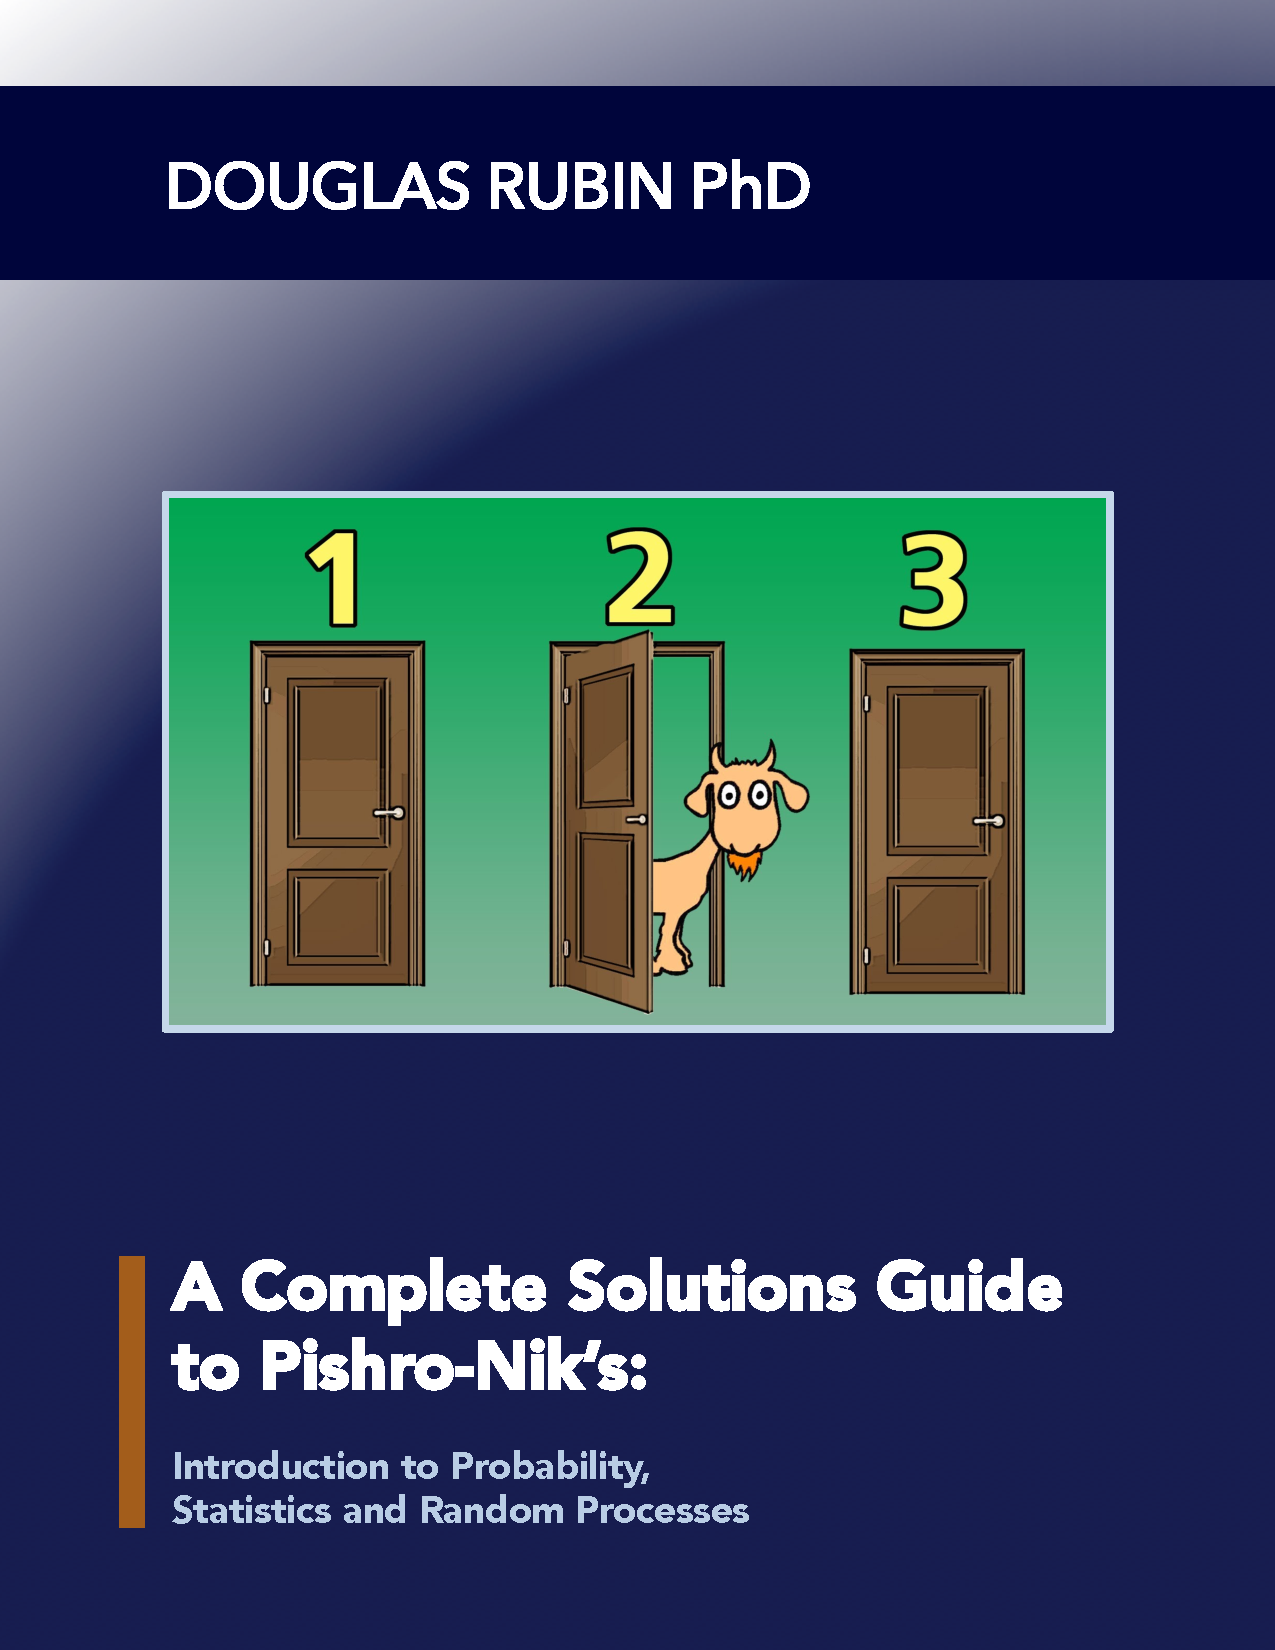
\includegraphics[totalheight=11in]{book_cover/book_cover.pdf}
	\end{figure}


%\newpage
\pagenumbering{arabic}  
\tableofcontents

\chapter{Basic Concepts}

 
\begin{problem}{1} $ $
	\begin{enumerate}
		
		\item 
			\begin{equation} 
				A \cup B = \{1, 2, 3\} \cup \{2, 3, 4, 5, 6, 7 \} =  \{1, 2, 3, 4, 5, 6, 7 \}  \nonumber
			\end{equation}
		
		\item 
			\begin{align}
				(A \cup C) - B &= \{1, 2, 3\} \cup \{ 7, 8, 9, 10\} -  \{2, 3, 4, 5, 6, 7 \} \nonumber \\
				&=  \{1, 2, 3, 7, 8, 9, 10\} -  \{2, 3, 4, 5, 6, 7 \} \nonumber \\
				& = \{ 1, 8, 9, 10\} \nonumber
			\end{align}
			
		\item 
			\begin{align}
				\bar A \cup (B-C) & = (\{1, 2, \ldots, 10 \}-A) \cup \left (\{2, 3, 4, 5, 6, 7 \} - \{7, 8, 9, 10 \} \right) \nonumber \\
				&= \{4, 5, 6, 7, 8, 9, 10\} \cup \{ 2, 3, 4, 5, 6 \} \nonumber \\
				& = \{2, 3, \ldots, 10 \} \nonumber
			\end{align}
			
		\item No, $A$, $B$ and $C$ do not partition $S$ since $2, 3 \in A$ as well as in $B$.  7 is also in both $B$ and $C$.		

	\end{enumerate}
\end{problem}



\begin{problem}{2} $ $
	\begin{enumerate}
		
		\item 
			\begin{equation} 
				[6, 8]\cup [2, 7)= [2, 8] \nonumber
			\end{equation}
		
		\item 
			\begin{equation} 
				[6, 8]\cap [2, 7)= [6, 7) \nonumber
			\end{equation}
			
		\item 
			\begin{equation} 
				[0, 1]^c = (-\infty, 0) \cup (1, \infty) \nonumber
			\end{equation}
		\item
			\begin{equation} 
				[6, 8] - (2, 7) = [7, 8] \nonumber
			\end{equation} 

	\end{enumerate}
\end{problem}


\begin{problem}{3} $ $
	\begin{enumerate}
		
		\item 
			\begin{align} 
				(A \cup B) - (A \cap B) & =  \nonumber\\
				& =(A \cup B) \cap (A \cap B)^c  \nonumber\\
				&= (A \cup B) \cap (A^c \cup B^c),\nonumber
			\end{align}
			where I have used De Morgan.
			
		\item
			\begin{equation} 
				B-C = B \cap C^c \nonumber
			\end{equation} 

		\item
			\begin{equation} 
				(A\cap C)\cup(A \cap B) \nonumber
			\end{equation} 
	
		\item
			\begin{equation} 
				(C-A-B)\cup ((A\cap B)-C) \nonumber
			\end{equation} 


	\end{enumerate}
\end{problem}



\begin{problem}{4} $ $
	\begin{enumerate}
		
		\item 
			\begin{equation} 
				A = \{(H,H), (H,T) \} \nonumber
			\end{equation}
			
		\item 
			\begin{equation} 
				B = \{ (H, T), (T,H), (T,T) \} \nonumber
			\end{equation}
			
		\item 
			\begin{equation} 
				C = \{ (H, T), (T,H) \} \nonumber
			\end{equation}


	\end{enumerate}
\end{problem}


\begin{problem}{5} $ $
	\begin{enumerate}
		
		\item $|A_2|$ is half of the numbers from 1 to 100, so $|A_2| = 50$.  To solve for $|A_3|$ note that there are 2 numbers between each pair of elements in $A_3$ where $A_3$ is assumed to be pre-sorted (e.g., 4, 5 are between 3 and 6).  There are also $|A_3|-1$ of these pairs, and thus $|A_3| + 2(|A_3|-1)+ 3 =100$, where I have added 3 to account for the numbers at the beginning and end of the sequence which are not divisible by 3 (1, 2 and 100).  Thus, I find that $|A_3| = 33$.  $|A_4|$ is exactly half of $|A_2|$, and thus $|A_4|=25$.  Finally, to solve for $|A_5|$ we may use the same method we used to solve for $|A_3|$:  $|A_5|+4(|A_5|-1) +4 =100$, from which we find that $|A_5| = 20$.
		
		\item By inclusion-exclusion:
			\begin{equation}
				|A_2\cup A_3 \cup A_5| = |A_2|+|A_3|+|A_5|-|A_2 \cap A_3| -|A_2 \cap A_5| - |A_3 \cap A_5| + |A_2 \cap A_3 \cap A_5| \nonumber .
			\end{equation}
Note that $|A_2 \cap A_3| = |A_{6}| = 16 $, $|A_2 \cap A_5| = |A_{10}| = 10 $, $|A_3 \cap A_5| = |A_{15}| = 6$, where $|A_{10}|$ and $|A_{15}|$ were found by counting (since there are very few elements in these sets), and $|A_6|$ was found by the same method I used to compute $|A_3|$.  Lastly, the intersection of all 3 sets is given by the set of multiples of 30, so that $|A_2 \cap A_3 \cap A_5| = |\{ 30, 60, 90\}| =3$.  Therefore: $|A_2\cup A_3 \cup A_5| =50+33+20 - 16-10-6+3=74$.

  
 	\end{enumerate}
\end{problem} 
  

\begin{problem}{6} From the following figure, it is clear that $|B| = 10+20+15=45$.
	  
	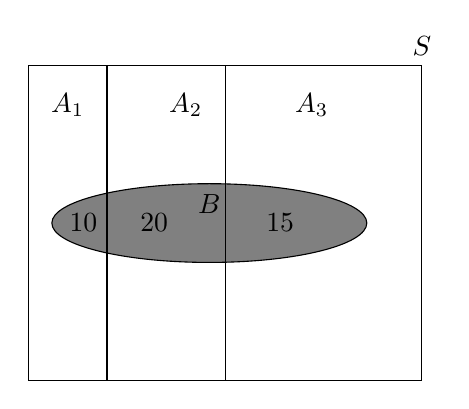
\begin{tikzpicture}[fill=gray]
		\filldraw[color=black, fill=gray] (0.3,0) ellipse (2. and 0.5) node [text=black,above] {$B$};
		\node[] at (-1.5,1.5) {$A_1$};
		\node[] at (0,1.5) {$A_2$};
		\node[] at (1.6,1.5) {$A_3$};
		\node[] at (-1.3,0) {$10$};
		\node[] at (-.4,0) {$20$};
		\node[] at (1.2,0) {$15$};
		\draw (-1.,-2) -- (-1.,2) ;
		\draw (0.5,-2) -- (0.5,2);
		\draw (-2,-2) rectangle (3,2) node[text=black,above] {$S$};
	\end{tikzpicture}
	
\end{problem} 


\begin{problem}{7} $ $
	\begin{enumerate}
		
		\item $A$ is a subset of a countable set, $\mathbb N$, and is thus countable.
		
		\item As shown in the book, if we can write any set, $S$ in the form:
		
		\begin{equation}
		S = \bigcup_{i \in \mathcal{B}} \bigcup_{j \in \mathcal C}  \{ q_{ij} \},
		\end{equation}
		where $\mathcal B$ and $\mathcal C$ are countable sets, then $S$ is a countable set.  It is easy to see that we may re-write $B$ as:
		
		\begin{equation}
		B = \bigcup_{i \in \mathbb Q} \bigcup_{j \in \mathbb Q}  \{ a_i +b_j \sqrt{2}\},
		\end{equation}
		where $q_{ij} \equiv a_i +b_j \sqrt{2}$, and thus $B$ is countable.
		
		
		\item $C$ is uncountable.  One way to prove this is to note that for all $x\in [0, 1]$, $(x, 0) \in C$, so that $C \supset [0, 1]$, i.e, $C$ is a superset of an uncountable set and is thus uncountable.
  
 	\end{enumerate}
\end{problem} 


\begin{problem}{8} I first prove that $A_n \subset A_{n+1}$ (a proper subset) for all $n=1, 2, \ldots$.  To do this, it suffices to prove that $(n-1)/n < n/(n+1)$, which I do with proof by contradiction.  By assuming $(n-1)/n \ge n/(n+1)$, after a little algebra, one concludes that $-1 \ge 0$, which is clearly a contradiction and therefore $(n-1)/n < n/(n+1)$. Thus the union of all the $A_n$s is given by the largest set in the sequence, which is $A_\infty$ ($=\lim_{n \rightarrow \infty} [0, \frac{n-1}{n})$).  After applying L'hopitals rule, one can show that $A_\infty = [0, 1)$, and thus:

	\begin{equation}
		A = \bigcup_{n=1}^{\infty} A_n = [0, 1) \nonumber .
	\end{equation}

  \end{problem} 
  
  
  \begin{problem}{9} As with the previous problem, one may show that $A_{n+1} \subset A_{n}$ for all $n=1, 2, \ldots$ by proving that $1/(n+1)<1/n$.  This is somewhat obvious, but if you really want to be formal, you can prove it with a proof by contradiction.  Therefore, the intersection of all the $A_n$s is given by the smallest set, $A_\infty$, which is $\lim_{n \rightarrow \infty} [0, \frac{1}{n}) = [0, 0) = \{ 0\}$, and thus:
	\begin{equation}
		A = \bigcap_{n=1}^{\infty} A_n = \{ 0\} \nonumber .
	\end{equation}
  \end{problem} 
  
  
    \begin{problem}{10} $ $
    \begin{enumerate}
    \item To motivate the bijection (the one-to-one mapping between $2^{\mathbb N}$ and $C$) we are about to construct, note that for every set in $2^{\mathbb N}$, a natural number $n$ will either appear once, or not at all.  Therefore, it is convenient to indicate its presence in the set with a 1 and its absence with a 0.  For example $\{1, 3, 6 \}$ will get mapped to the sequence $101001000 \ldots$ (this is implicitly assuming that we have pre-ordered the elements in the particular set from $2^{\mathbb N}$).  In general, the bijective mapping we use $f: 2^{\mathbb N} \rightarrow C$, is given by:
    \begin{equation*}
    f(x) = \mathbbm{1}(1\in x)\mathbbm{1}(2\in x) \ldots,
    \end{equation*}
    where $\mathbbm{1}$ is the so-called indicator function which is 1 if its argument evaluates to true and 0 otherwise.  To prove that this mapping is bijective, we must prove it is both injective and surjective.
 
 To prove it is injective, I use a proof by contradiction.  Assume it is not injective.  Under this assumption there exists $x, x^\prime \in 2^{\mathbb N}$, where $x\neq x^\prime$ such that $f(x) = f(x^\prime)$.  $x$ and $x^\prime$ can either have the same cardinality, or they can be different.  Without loss of generality, if they are different, let us call $x$ the one with the larger cardinality.  Since $x \neq x^\prime$ there exists at least 1 natural number $n$ in $x$ which is not in $x^\prime$.  Therefore in the sequences $f(x)$ and $f(x^\prime)$, there is at least one value in the sequences which does not match up, namely the value at position $n$, and therefore $f(x) \neq f(x^\prime)$, which violates our original assumption.
 
 The proof of surjectivity is also straightforward.
     
     \item Any number in $x \in [0, 1)$ always has a unique binary expansion given by $x = b_1/2+b_2/2^2+...$, and therefore we can construct a bijective mapping between $x \in [0, 1)$ and $C$ by computing $b_1/2+b_2/2^2+...$, and then by dropping the 0. at the beginning of the sequence.  Since there is a bijection between $2^{\mathbb N}$ and $C$ and a bijection between $C$ and $[0, 1)$ (and given the fact that the composition of 2 bijections is a bijection) there is thus a bijection between $2^{\mathbb N}$ and $[0, 1)$.  Assuming (correctly so) that the interval $[0, 1)$ is uncountable, then so too is $2^{\mathbb N}$.
     
     
     
     \end{enumerate}
     
  \end{problem} 
  
  
    \begin{problem}{11} $ $
 As shown in the previous problem, there is a bijection between $[0, 1)$ and $C$.  Therefore, if $C$ is uncountable, then so too is $[0, 1)$.  We can use what is known as Cantor's diagonal argument to prove that $C$ is uncountable.
 
 Let us try to search for a bijective mapping between $C$ and $\mathbb N$.  Suppose, for example, that the first few mappings are given by:
 \\

 \begin{tabular}{ c c c }
1 & $\rightarrow$ & $\mathbf{0} 000000\ldots$ \\
2 & $\rightarrow$& $1\mathbf{1}11111\ldots$\\
3 & $\rightarrow$& $01 \mathbf{0}1010\ldots$\\
4& $\rightarrow$ &$101\mathbf{0}101\ldots$\\
5 & $\rightarrow$&$1101\mathbf{0}11\ldots$\\
6& $\rightarrow$&$00110\mathbf{1}1\ldots$\\
7 &$\rightarrow$& $100010\mathbf{0}\ldots$ \\
& $\vdots$&  
 \end{tabular}


Let us now construct a new sequence, $s \in C$ by enumerating the complement of the elements along the diagonal of the mapping (which I have highlighted in boldface above), $s = 1011101 \ldots$.  By construction, $s$ differs from every proposed mapping since the $n^{th}$ digit in $s$ is different than the $n^{th}$ digits in all of the mappings.   Thus, no natural number gets mapped to $s$, and hence the proposed mapping is not surjective.  The mappings I chose for illustration in this example for $1, \ldots, 7$ were arbitrary, and this argument applies to any potential mapping.  Therefore, there is no bijective mapping between $\mathbb N$ and $C$, and hence no bijection between $[0, 1)$ and $\mathbb N$.  Thus, the interval $[0, 1)$ is uncountable.
 
 
  \end{problem}
  
\begin{problem}{12} $ $
	\begin{enumerate}
		
		\item The domain is $\{ H, T \}^3$ and the codomain is $\mathbb N \cup \{ 0 \}$
		
		\item $range(f) = \{0, 1, 2, 3\}$
		
		\item $x$ can be all triplets that contain exactly 2 heads: $(H, H, T)$, $(H, T, H)$ or $(T, H, H)$.
  
 	\end{enumerate}
\end{problem} 


\begin{problem}{13} $ $
	\begin{enumerate}
		
		\item The universal set is partitioned by the events $a$, $b$, $d$, and thus $P(b) = 1 - P(a) - P(d) = 1-0.5-0.25=0.25$.
		
		\item Since the events $b$ and $d$ are disjoint, by the 3rd axiom of probability, $P(b \cup d) = P(b)+P(d) = 0.25+0.25 = 0.5 $.
	
  
 	\end{enumerate}
\end{problem} 


\begin{problem}{14} $ $
	\begin{enumerate}
		
		\item By inclusion-exclusion: $P(A \cap B) = P(A)+P(B)-P(A \cup B) = 0.4+0.7-0.9 = 0.2$.
		
		\item 
			\begin{align*}
				P(A^c \cap B) &= P(B-A) \\
				& = P(B) - P(A\cap B) \\
				& = 0.7-0.2 \\
				&=0.5
			\end{align*}
			
		\item 
			\begin{align*}
				P(A-B) & = P(A) - P(A\cap B) \\
				& = 0.4-0.2 \\
				&=0.2
			\end{align*}
			
		\item  By drawing the Venn diagram, one can see that
			\begin{align*}
				P(A^c-B) & = P(S) - P(A\cup B) \\
				& = 1 - 0.9 \\
				&=0.1,
			\end{align*}
		where $S$ is the universal set.
		
		
		\item  By drawing the Venn diagram, one can see that
			\begin{align*}
				P(A^c \cup B) & = P(S) - P(A- B) \\
				& = 1 - 0.2 \\
				&=0.8.
			\end{align*}

		\item  
			\begin{align*}
				P(A \cap (B \cup A^c)) &=  P((A \cap B)\cup(A \cap A^c) )\\
				& = P((A \cap B) \cup \emptyset)\\
				&= P(A \cap B) \\
				& = 0.2.
			\end{align*}
  
 	\end{enumerate}
\end{problem} 



  \begin{problem}{15} $ $
	\begin{enumerate}
		
		\item The second roll is independent of the first, so we only need to consider the second roll, in which case $P(X_2 = 4) = 1/6$ since this is a finite sample space with equal probabilities for all outcomes.
		
	\item The sample space is $\{1, 2, \ldots, 6 \} \times \{1, 2, \ldots, 6 \}$, which has a cardinality of 36, and the possible outcomes corresponding to the event that $X_1 +X_2 = 7$ are given by the set \\
	$\{ (1, 6), (6, 1), (2, 5), (5, 2), (3, 4), (4, 3) \}$, which has a cardinality of 6, and therefore $P(X_1+X_2 = 7) = 6/36=1/6$.
		
		\item Listing out the tuples that satisfy the second condition in a matrix-like representation, we have: 
		
			\begin{equation*}
				\begin{array}{ccc}
					(1, 4) & (1, 5)& (1, 6) \\
					(2, 4) & (2, 5)& (2, 6) \\
 					& \vdots & \\
					(6, 4) & (6, 5) & (6, 6) \\
				\end{array},
			\end{equation*}
of which there are $3\times 6$ elements.  However, the first condition does not allow the elements $(2, 4)$, $(2, 5)$, $(2, 6)$, and thus the total size of the event space is  $3\times 6-3 =15$.  Thus $P(X_1 \ne 2 \cap X_2 \ge 4) = 15/36=5/12$.
	
  
 	\end{enumerate}
\end{problem} 


\begin{problem}{16} $ $
	\begin{enumerate}
		
		\item The formula for a geometric series will be useful here: $\sum_{k=0}^{\infty} c r^k = a/(1-r)$ for $|r|<1$.  To solve for $c$, we can use the normalization constraint:
		
		\begin{align*}
			1 &= \sum_{k=1}^{\infty} P(k) \\
			& = -c+\sum_{k=0}^{\infty} c\left (\frac{1}{3} \right)^k \\
			& = -c +\frac{c}{1-1/3}, 
		\end{align*}
and therefore $c=2$.

		\item 
			\begin{align*}
			P(\{ 2, 4, 6\}) &=P(\{2 \} \cup \{ 4 \} \cup \{6\}) \\
			& = P(2)+P(4)+P(6) \\
			& =2\left[\frac{1}{3^2}+ \frac{1}{3^4}+\frac{1}{3^6}\right] \\
			& = \frac{182}{729}
			\end{align*}
			
		\item 
			\begin{align*}
			P(\{ 3, 4, 5, \ldots \}) &= 2\sum_{k=3}^{\infty} \left( \frac{1}{3}\right)^k \\
			&= -2\left[1+\frac{1}{3} +\frac{1}{9} \right]+ 2\sum_{k=0}^{\infty} \left( \frac{1}{3}\right)^k \\
			& = - 2 \left( \frac{13}{9} \right) +2\left(\frac{3}{2}\right) \\
			& =\frac{1}{9}
			\end{align*}
  This answer may also have been computed $1-P(1)-P(2)$.
 	\end{enumerate}
\end{problem} 



\begin{problem}{17} Let us write down what we know in equations.  Let $a$, $b$, $c$, $d$ represent the events that teams, A, B, C and D win the tournament respectively.  Then as stated in the problem, $P(a) = P(b)$, $P(c)=2P(d)$ and $P(a \cup c)=0.6$.  Since the events partition the sample space, $P(a \cup c)=P(a)+P(c)$.  We know one more equation, which is that the probabilities must sum to one: $P(a)+P(b)+P(c)+P(d)=1$.  We therefore have a linear system with 4 equations and 4 unknowns, and it will thus be convenient to write this in matrix notation in order to solve for the probabilities:

	\begin{equation*}
		  \begin{bmatrix}
			1 &-1&0&0\\
			0&0&1&-2 \\
			1&0&1&0 \\
			1&1&1&1
		  \end{bmatrix}
 		 \begin{bmatrix}
			P(a)\\
			P(b)\\
			P(c)\\
			P(d)
		  \end{bmatrix}
		  =
		  \begin{bmatrix}
			0 \\
			0 \\
			0.6 \\
			1
		  \end{bmatrix}.
	\end{equation*}
	
$\implies$
	
	\begin{align*}
 		 \begin{bmatrix}
			P(a)\\
			P(b)\\
			P(c)\\
			P(d)
		  \end{bmatrix}
		  & =
		  \begin{bmatrix}
			1 &-1&0&0\\
			0&0&1&-2 \\
			1&0&1&0 \\
			1&1&1&1
		  \end{bmatrix}^{-1}
		  \begin{bmatrix}
			0 \\
			0 \\
			0.6 \\
			1
		  \end{bmatrix} \\
		  & =  \begin{bmatrix}
			2 &1&-3&2\\
			1&1&-3&2 \\
			-2&-1&4&2 \\
			-1&-1&2&-1
		  \end{bmatrix}
		  \begin{bmatrix}
			0 \\
			0 \\
			0.6 \\
			1
		  \end{bmatrix}\\
		  &=
		  \begin{bmatrix}
			0.2 \\
			0.2 \\
			0.4 \\
			0.2
		  \end{bmatrix}.
	\end{align*}
Notice that, as required, the probabilities sum to 1.

\end{problem} 

\begin{problem}{18} $ $
	\begin{enumerate}
		\item $P(T \le 1) = \frac{1}{16}$
		
		\item 
			\begin{align*}
				P(T>2) &= 1 - P(T\le 2) \\
				&= 1-\frac{4}{16} \\
				&=\frac{3}{4}
			\end{align*}
			
		\item
			\begin{align*}
				P(1\le T \le 3) &= P(T \le 3) - P(T < 1) \\
				&= \frac{9}{16}-\frac{1}{16} \\
				&=\frac{1}{2}
			\end{align*}
			
  
 	\end{enumerate}
\end{problem} 

\begin{problem}{19} The solutions to the quadratic are given by the quadratic formula:

	\begin{equation}
		X = \frac{-1 \pm \sqrt{1-4AB}}{2A},
	\end{equation}
	which has real solutions iff the condition $1-4AB \ge 0$ is satisfied.  We therefore seek the probability that $P(1-4AB\ge 0)$ (in the unit square), which, since the point $(A, B)$ is picked uniformly, is the fraction of area in the unit square which satisfies this constraint.  Therefore points which satisfy the following inequalities contribute to this probability:

	\begin{equation*}
		\frac{1}{4} \left(\frac{1}{x} \right)\ge y,
	\end{equation*}
	
	\begin{equation*}
		x\le1
	\end{equation*}
	and
		\begin{equation*}
		y\le1,
	\end{equation*}
where the last 2 inequalities follow since the randomly drawn points must lie within the unit square.  The area in the unit square which satisfies these constraints is shown in Fig.~\ref{fig:prob_19}.


	\begin{figure}[t]
	\centering
      		 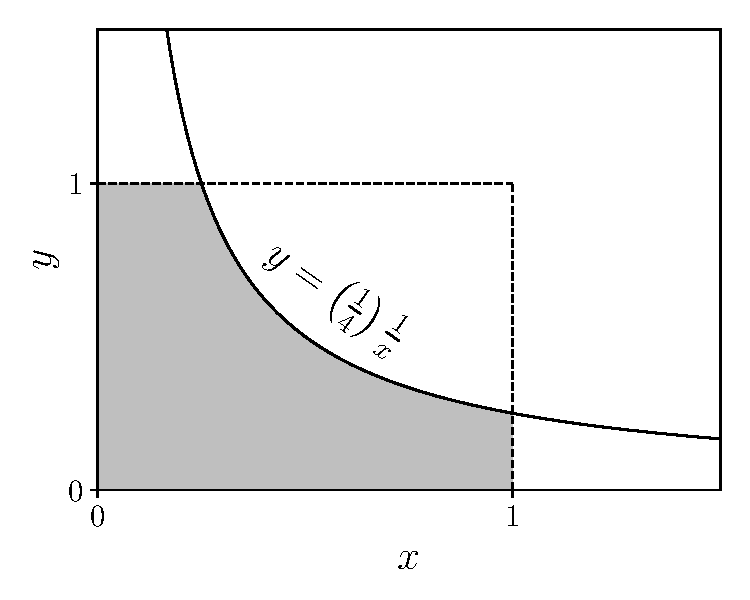
\includegraphics[totalheight=6cm]{chpt1/prob19.pdf}
  			  \caption{area of unit square resulting in real solutions}
    			   \label{fig:prob_19}
	\end{figure}
It is clear from the figure that the area is given by:

\begin{align*}
	P(\mathrm{real~solns.}) & = \frac{1}{4} +\frac{1}{4}\int_{1/4}^1\frac{1}{x} dx \\
	& = \frac{1}{4}+\frac{1}{4} \ln 4 \\
	& \approx 0.60.
\end{align*}
	
\end{problem} 


\begin{problem}{20} $ $

\begin{enumerate}
\item To solve this problem, note that:
	\begin{equation*}
		A\equiv \bigcup_{i=1}^{\infty}A_i = A_1 \cup (A_2-A_1) \cup (A_3-A_2) \cup \ldots, 
	\end{equation*}
where in the figure, $A_1$ is the innermost circle, $(A_2-A_1)$ is the ``annulus" around $A1$, $(A_3-A_2)$ is the next ``annulus" and so-forth.  It is clear that the union of $A_1$ and all of the annuli results in $A$, and that each of these regions are also disjoint.  I utilize the previous equation in the desired proof:
	\begin{figure}[t]
	\centering
      		 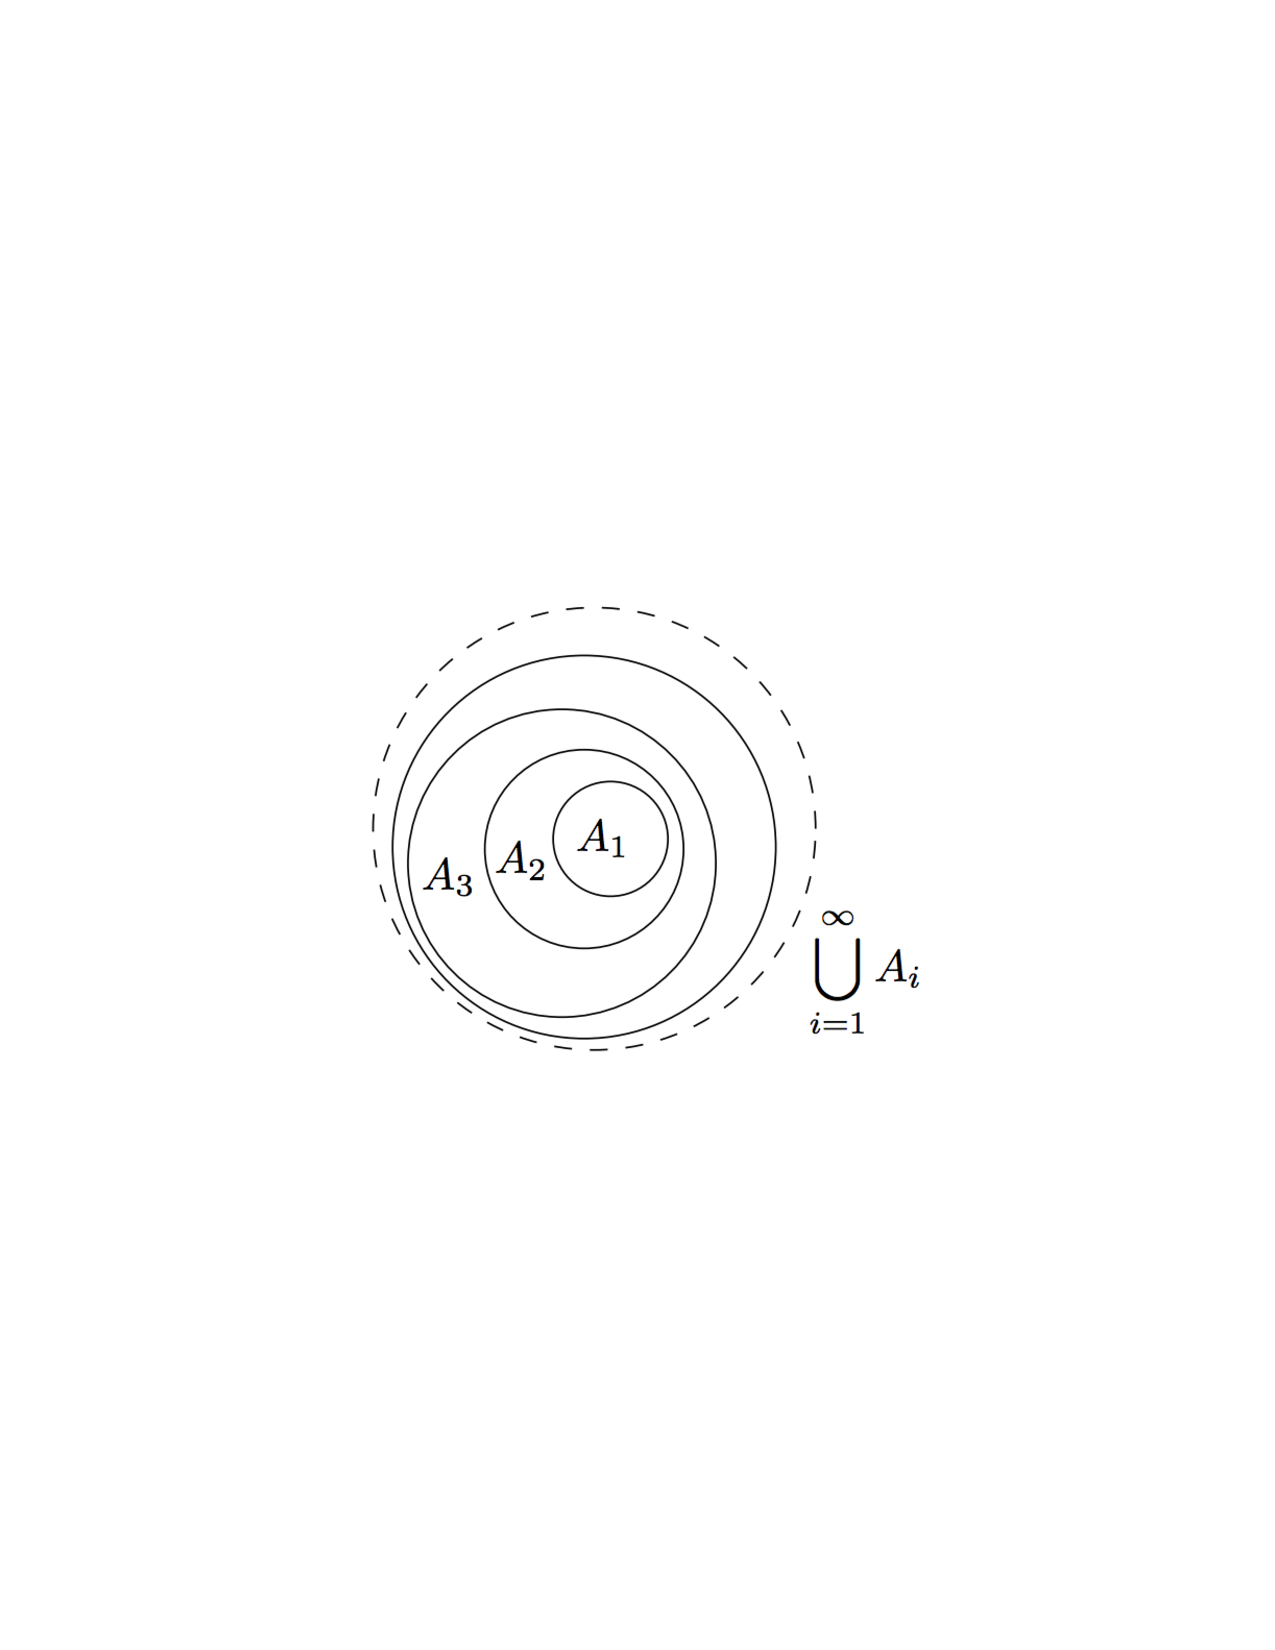
\includegraphics[totalheight=6cm]{chpt1/prob20.pdf}
  			  \caption{Venn diagram of events $A_1, A_2, \ldots$}
    			   \label{fig:prob_20}
	\end{figure}
	
	\begin{proof}
		\begin{align*}
		P(A) & = P(A_1)+\sum_{i=2}^{\infty} P(A_i-A_{i-1}) \\
		& = P(A_1)+\lim_{n \rightarrow \infty} \sum_{i=2}^{n} P(A_i-A_{i-1}) \\
		& = P(A_1)+\lim_{n \rightarrow \infty} \sum_{i=2}^{n} \left [P(A_i)-P(A_{i-1}) \right] \\
		& =  P(A_1)+\lim_{n \rightarrow \infty} \{ [P(A_2)-P(A_1)]+[P(A_3)-P(A_2)]+[P(A_4)-P(A_3)] \\
		& +\ldots +[P(A_n)-P(A_{n-1})]\} \\
		& = P(A_1)+\lim_{n \rightarrow \infty} [P(A_n)-P(A_1)] \\
		& = \lim_{n \rightarrow \infty} P(A_n) \qedhere
		\end{align*}
	\end{proof}
	
	\item Redefining $A$: $A\equiv \bigcap_{i=1}^{\infty}A_i$, we seek to find $P(A)$. If $A_1, A_2, \ldots$ is a series of decreasing events, then $A_1^c, A_2^c, \ldots$ must be a series of increasing events, and we can can therefore utilize the results of the part (a) on sequence of the complements (as well as De Morgan):
	
	\begin{align*}
		P(A^c) = P\left(\left(\bigcap_{i=1}^{\infty}A_i\right)^c\right)=P\left(\bigcup_{i=1}^{\infty}A_i^c\right) = \lim_{n \rightarrow \infty}P(A_n^c).
	\end{align*}
	
	A few more steps completes the proof:
	
		\begin{proof}
		\begin{align*}
		P(A) & = 1-P(A^c) \\
		& = 1 - \lim_{n \rightarrow \infty}P(A_n^c) \\
		& = \lim_{n \rightarrow \infty} [1 - P(A_n^c)]\\
		 & = \lim_{n \rightarrow \infty} P(A_n) \qedhere
		\end{align*}
	\end{proof}
	
	
\end{enumerate}
	
\end{problem} 

\begin{problem}{21} $ $
	\begin{enumerate}
		\item
			Let us define new events, $B_i$, such that $B_1$ =$A_1$, $B_2 =A_2-A_1$, $B_3= A_3-A_2-A_1, \ldots$.  Note that the $B_i$s are disjoint.  Also note that:
			
			\begin{align*}
			\bigcup_{i=1}^n B_i & = A_1 \cup (A_2-A_1) \cup (A_3-A_2-A_1) \cup \ldots  \cup (A_n-A_{n-1}-\ldots -A_1)\\
			&=A_1\cup A_2 \cup A_3 \ldots \cup A_n\\
			&=\bigcup_{i=1}^n A_i,
			\end{align*}
and for the same reason $\bigcup_{i=1}^\infty B_i=\bigcup_{i=1}^\infty A_i$.  Using these facts, the proof is now straightforward:

		\begin{proof}
		\begin{align*}
		P\left(\bigcup_{i=1}^\infty A_i \right) &= P\left(\bigcup_{i=1}^\infty B_i\right) \\
		& = \sum_{i=1}^\infty P(B_i) \\
		& = \lim_{n \rightarrow \infty} \sum_{i=1}^n P(B_i) \\
		& = \lim_{n \rightarrow \infty} P\left (\bigcup_{i=1}^n B_i \right) \\
		& = \lim_{n \rightarrow \infty} P\left (\bigcup_{i=1}^n A_i \right)  \qedhere
		\end{align*}
	\end{proof}
	
	\item The prove this second result I use the previous result as well as De Morgan (twice):
	
		\begin{proof}
		\begin{align*}
		P\left (\bigcap_{i=1}^\infty A_i \right) &= P\left( \bigcup_{i=1}^\infty A_i^c \right) \\
		& = \lim_{n \rightarrow \infty} P\left(\bigcup_{i=1}^n A_i^c \right) \\
		& =\lim_{n \rightarrow \infty} P\left(\bigcap_{i=1}^n A_i\right)  \qedhere
		\end{align*}
	\end{proof}
			
	\end{enumerate}

\end{problem} 


\begin{problem}{22} Let $A_{coff}$ be the event that a customer purchases coffee and $A_{cake}$ be the event that a customer purchases cake.  We know that $P(A_{coff}) = 0.7$, $P(A_{cake}) = 0.4$ and $P(A_{coff}, A_{cake}) = 0.2$.  Thus, the conditional probability we seek is:

	\begin{equation*}
		P(A_{coff}|A_{cake}) = \frac{P(A_{coff}, A_{cake})}{P(A_{cake}) } = \frac{0.2}{0.4}=0.5.
	\end{equation*}

\end{problem} 

\begin{problem}{23} $ $
	\begin{enumerate}
		\item 
			\begin{equation*}
				P(A|B) = \frac{P(A \cap B)}{P(B)} = \frac{0.1+0.1}{0.1+0.1+0.1+0.05} \approx 0.57
			\end{equation*}
			
		\item 
			\begin{equation*}
				P(C|B) = \frac{P(C \cap B)}{P(B)} = \frac{0.1+0.05}{0.1+0.1+0.1+0.05} \approx 0.43
			\end{equation*}
			
		\item 
			\begin{equation*}
				P(B|A \cup C) = \frac{P(B\cap ( A\cup C))}{P( A\cup C)} = \frac{0.1+0.1+0.05}{0.1+0.2+0.1+0.1+0.05+0.15} \approx 0.36
			\end{equation*}
			
		\item 
			\begin{equation*}
				P(B|A, C) = \frac{P(B \cap (A \cap C))}{P(A \cap C)} = \frac{0.1}{0.1+0.1} =0.5
			\end{equation*}
		
	\end{enumerate}

\end{problem} 



\begin{problem}{24} $ $
	\begin{enumerate}
		\item 
			\begin{equation*}
				P(2 \le X \le 5) = \frac{3}{10} =0.3
			\end{equation*}
			
		\item 
			\begin{equation*}
				P(X \le 2| X \le 5) = \frac{2}{5} =0.4
			\end{equation*}
		
		\item 
			\begin{equation*}
				P(3 \le X \le 8| X \ge 4) = \frac{P(3 \le X \le 8 \cap X \ge 4)}{P(X \ge 4)} = \frac{4}{6} = \frac{2}{3}
			\end{equation*}		
		
	\end{enumerate}

\end{problem} 


\begin{problem}{25} Let $ON$ denote the event that a student lives on campus, $OFF$ denote the event that a student lives off campus and $A$ denote the event that a student receives an A.  Given the data I compute the following probabilities:

\begin{equation*}
P(ON) \approx \frac{200}{600} =\frac{1}{3}
\end{equation*}

\begin{equation*}
P(A) \approx \frac{120}{600} =\frac{1}{5}
\end{equation*}

\begin{equation*}
P(A \cap ON) = P(A) - P(A \cap OFF) \approx \frac{1}{5} - \frac{80}{600} = \frac{1}{15}
\end{equation*}

If the events $ON$ and $A$ are independent, then $P(A \cap ON)  = P(A)P(ON)$.  Looking at the probabilities above, we see that the data suggests this relationship, and thus the data suggests that getting an A and living on campus are independent. 

\end{problem} 


\begin{problem}{26}  Let $N_1$ be the number of times out of $n$ that a 1 is rolled, $N_6$ be the number of times out of $n$ that a 6 is rolled and $X_i$ be the value of the $i^{th}$ roll.  Then:

\begin{align*}
	P(N_1 \ge 1 \cap N_6 \ge 1) &= 1 - P((N_1 \ge 1 \cap N_6 \ge 1)^c) \\
	&= 1 - P(N_1= 0 \cup N_6=0) \\
	& = 1-[P(X_1 \ne 1, X_2 \ne 1, \ldots, X_n \ne 1)+P(X_1 \ne 6, X_2 \ne 6, \ldots, X_n \ne 6) \\
	& - P((X_1 \ne 1, X_2 \ne 1, \ldots, X_n \ne 1)\cap (X_1 \ne 6, X_2 \ne 6, \ldots, X_n \ne 6))] \\
	& =1-\left [ \left (\frac{5}{6} \right )^n+\left (\frac{5}{6}\right)^n - P(X_1 \ne 1, X_1 \ne 6, X_2 \ne 1, X_2 \ne 6, \ldots, X_n \ne 1 X_n \ne 6)\right] \\
	& =1-\left [2 \left (\frac{5}{6} \right )^n - P(X_1 \ne 1, X_1 \ne 6)^n \right] \\
	& = 1-\left [ 2\left (\frac{5}{6} \right )^n-\left (\frac{4}{6} \right )^n \right] \\
	& =1 - \frac{2(5^n) -4^n}{6^n}.
\end{align*}
In the second line I have used De Morgan, and I have also used the fact, several times, that the outcome of roll $i$ is independent of the outcome of roll $j$.  Testing for a for values of $n$, I find that, when $n=1$, the probability is 0, which makes sense because at the very minimum we would need at least one 1 and one 6, which cannot happen if we have only rolled once.  The probability then monotonically increases, which also makes sense because it becomes more and more likely that we roll at least one 1 and at least one 6 the more rolls we throw.  Note that as a sanity check, one can show that $\lim_{n \rightarrow \infty} 1 - (2(5^n) -4^n)/(6^n)$ is 1, so that our formula for the probability is bounded between 0 and 1.  Also note that this formula can also be obtained more easily with combinatorics, which will be introduced in Chapter 2.

\end{problem}

\begin{problem}{27} $ $
\begin{enumerate}
\item Refer to Fig.~\ref{fig:prob_27}
	\begin{figure}[t]
	\centering
      		 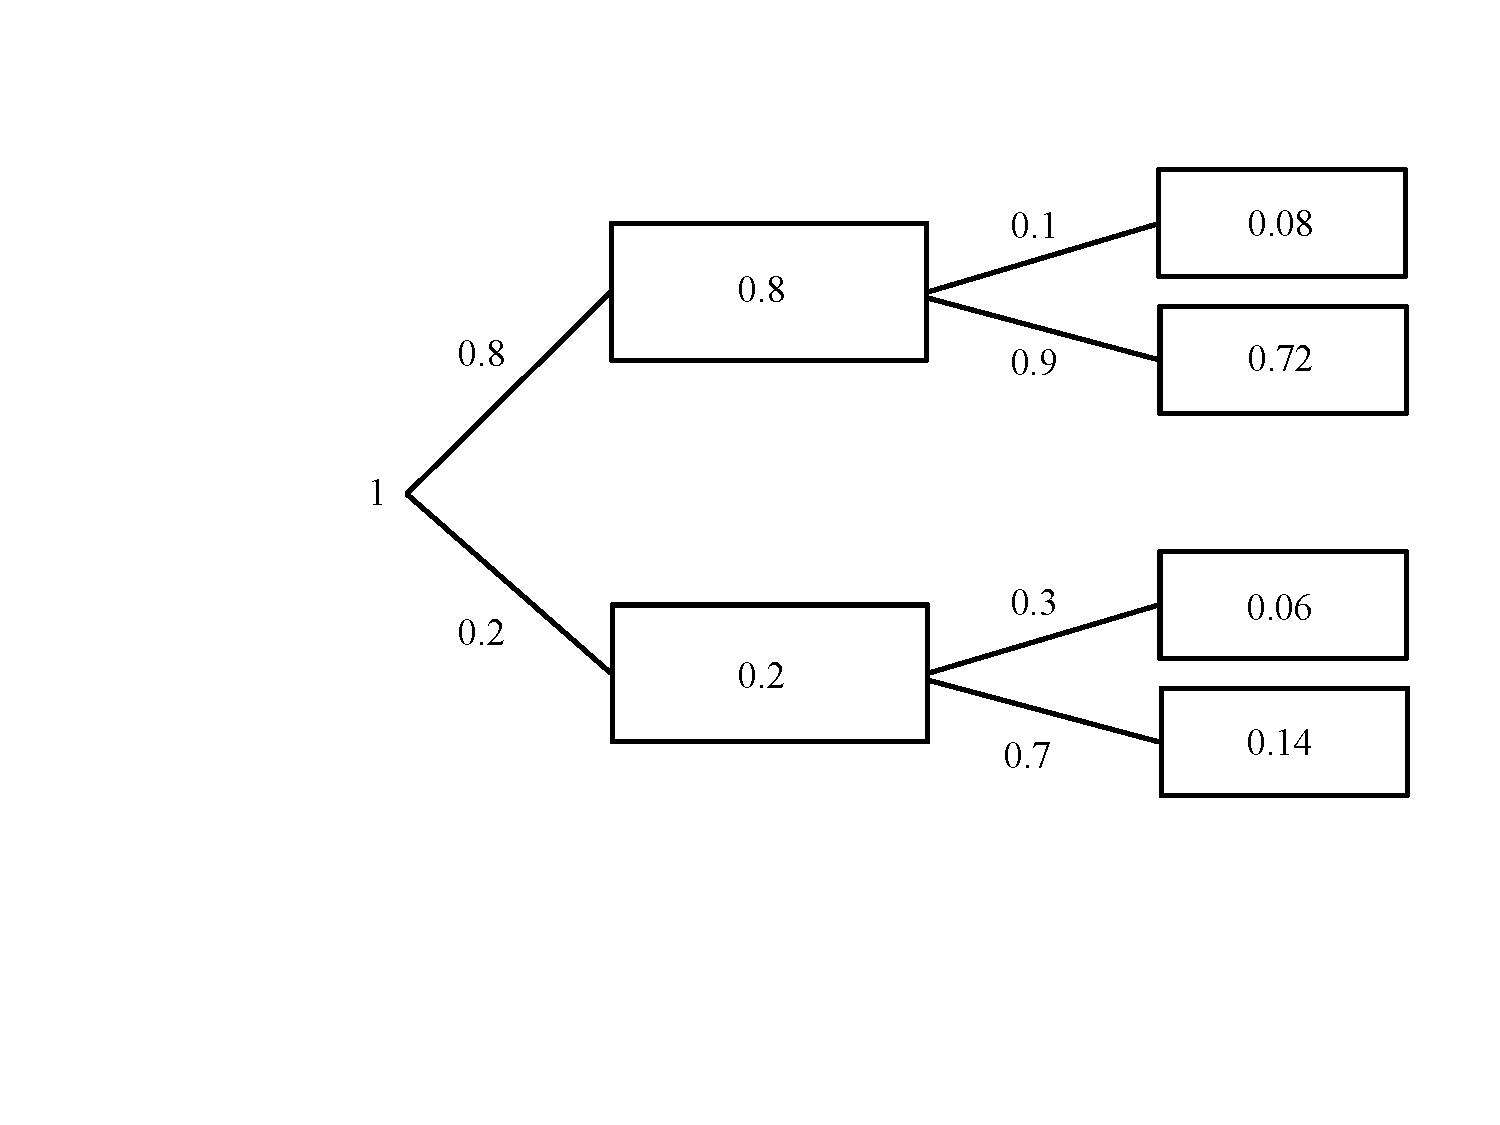
\includegraphics[totalheight=6cm]{chpt1/tree_27.pdf}
  			  \caption{Tree diagram for problem 27.}
    			   \label{fig:prob_27}
	\end{figure}
	
	\item $P(E) = P(E \cap G) + P(E \cap G^c) = 0.08+0.06=0.14$
	
	\item $P(G|E^c) = \frac{P(G \cap E^c)}{P(E^c)} =  \frac{0.72}{1-0.14} \approx 0.84$. 
	
\end{enumerate}

\end{problem}


\begin{problem}{28} Let $A_i$ be the event that the $i^{th}$ ($i=1, 2, 3$) unit of the 3 picks is defective, while the other 2 are not defective.  Note that $A_1$, $A_2$ and $A_3$ are all disjoint, since it is impossible for any unit to be both defective and not defective simultaneously.  The probability we seek is therefore:

\begin{align*}
P(A_1 \cup A_2 \cup A_3) & = P(A_1)+P(A_2)+P(A_3) \\
&= \left(\frac{5}{100}\right)\left(\frac{95}{99}\right)\left(\frac{94}{98}\right) +\left(\frac{95}{100}\right)\left(\frac{5}{99}\right)\left(\frac{94}{98}\right)+\left(\frac{95}{100}\right)\left(\frac{94}{99}\right)\left(\frac{5}{98}\right) \\
&\approx 0.14.
\end{align*}


\end{problem}




\begin{problem}{29} Let $F$ be the event that the system is functional, and $C_i$ be the event that component $i$ is functional.
	\begin{enumerate}
		\item $P(F) = P(C_1, C_2, C_3) = P_1 P_2 P_3$
		\item By inclusion-exclusion:
		\begin{align*} 
		P(F) &= P(C_1\cup C_2 \cup C_3) \\
		& = P_1+ P_2 +P_3 -P_1P_2-P_1P_3-P_2P_3+P_1P_2P_3
		\end{align*} 
		

		\item 
			\begin{align*}
				P(F) &= P((C_1, C_3) \cup (C_2, C_3)) \\
				& = P(C_1, C_3)+P(C_2, C_3) - P((C_1\cap C_3) \cap (C_2 \cap C_3)) \\
				& = P_1 P_3+P_2 P_3 - P(C_1, C_2, C_3) \\
				& = P_1 P_3+P_2 P_3 - P_1 P_2 P_3 
			\end{align*}
			
		\item $P(F) = P(C_1, C_2)+P(C_3) = P_1 P_2 +P_3 - P_1 P_2 P_3$
		\item $P(F) = P(C_1, C_2, C_5)+P(C_3, C_4, C_5) - P(C_1, C_2, C_3, C_4, C_5) = P_1 P_2 P_5+P_3 P_4 P_5 - P_1 P_2 P_3 P_4 P_5 $
	\end{enumerate}

\end{problem}
	
	
\begin{problem}{30} $ $
\begin{enumerate}
\item  The region in the unit square corresponding to set $A$ can be made more clear if we write the absolute value as a piecewise function:

\begin{equation*}
|x-y| \le \frac{1}{2} \implies
  \begin{cases}
                                   x-y \le \frac{1}{2} & \mathrm{if}~x \ge y \\
                                    y-x \le \frac{1}{2}  & \mathrm{if}~x<y \\

  \end{cases}
  \implies
  \begin{cases}
                                   y \ge - \frac{1}{2}+x & \mathrm{if}~y \le x \\
                                    y \le \frac{1}{2}+x  & \mathrm{if}~y>x \\

  \end{cases}.
\end{equation*}
This piecewise function, along with the fact that $A$ must be bounded in the unit square leads to hashed-in region in Fig.~\ref{fig:prob_30}.  The region corresponding to set $B$ is just the are in the unit square above the $45^\circ$ line (corresponding to the gray shaded region in Fig.~\ref{fig:prob_30}).

	\begin{figure}[t]
	\centering
      		 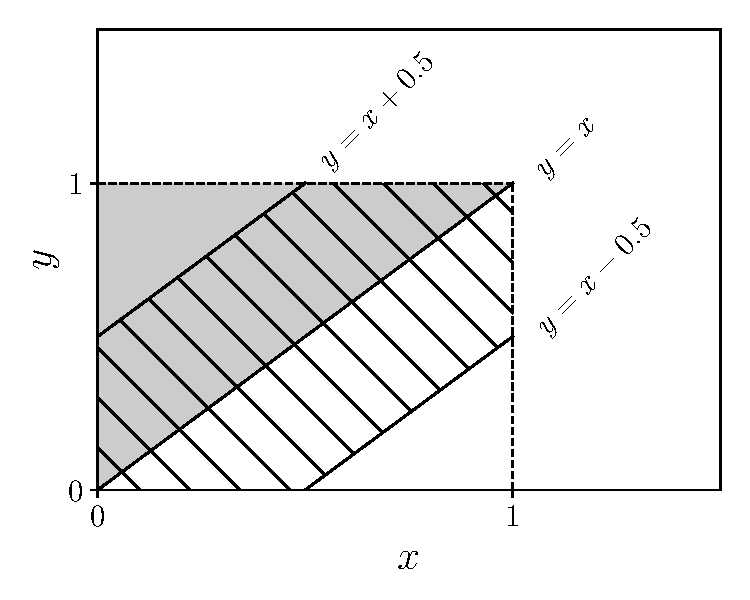
\includegraphics[totalheight=6cm]{chpt1/prob30.pdf}
  			  \caption{The unit square for Problem 30.  The shaded region represents the set $B$ and the hashed region represents the set $A$}
    			   \label{fig:prob_30}
	\end{figure}
	
\item Using a little geometry, I find: $P(A) = 1- 2\left (\frac{1}{2} \right)\left (\frac{1}{2} \right)\left (\frac{1}{2} \right) = \frac{3}{4}$ and $P(B)=\frac{1}{2}$.

\item Again, using some geometry, I find: $P(A\cap B) = \frac{1}{2} - \left (\frac{1}{2} \right)\left (\frac{1}{2} \right)\left (\frac{1}{2} \right) = \frac{3}{8}$.  Since $P(A)P(B) =  \left (\frac{3}{4} \right) \left (\frac{1}{2} \right) =\frac{3}{8}$, the 2 events are indeed independent.

\end{enumerate}

\end{problem}


\begin{problem}{31} $ $
\begin{enumerate}
\item  Let $s$ be the event that the received email is spam and $r$ be the event that the received email contains the word refinance.  From the problem statment, we know that $P(s) = 0.5$ (so that $P(s^c) = 0.5$), $P(r|s)=0.01$ and $P(r|s^c)= 0.00001$.  Using Bayes' rule:

\begin{align*}
P(s|r) &= \frac{P(r|s)P(s)}{P(r)} \\
&= \frac{P(r|s)P(s)}{P(r|s)P(s)+P(r|s^c)P(s^c)} \\
& = \frac{(0.01) (0.5)}{(0.01)(0.5)+(0.00001)(0.5)} \\
& \approx 0.999
\end{align*}

\end{enumerate}

\end{problem}

\begin{problem}{32} $ $

\begin{enumerate}

\item
There are 4 possible paths from $A$ to $B$: 1 to 4 (path 1), 2 to 5 (path 2), 1 to 3 to 5 (path 3), 2 to 3 to 4 (path 4).  Let $\mathcal P_i$ be the event that path $i$ is open.  Only 1 path needs to be open for event $A$ to occur, so the probability of $A$ is given by the probability of $\mathcal P_1$ or $\mathcal P_2$ or $\mathcal P_3$ or $\mathcal P_4$.  We expand this probability with inclusion-exclusion, making sure to enumerate all unique pairs and all unique triplets:

\begin{align*}
P(A)& = P(\mathcal P_1 \cup \mathcal P_2 \cup \mathcal P_3 \cup \mathcal P_4) \\
&= P(\mathcal P_1)+ P(\mathcal P_2)+P(\mathcal P_3)+P( \mathcal P_4) \\
&- P(\mathcal P_1\cap \mathcal P_2)-P(\mathcal P_1\cap \mathcal P_3)-P(\mathcal P_1\cap \mathcal P_4)-P(\mathcal P_2\cap \mathcal P_3)-P(\mathcal P_2\cap \mathcal P_4)-P(\mathcal P_3\cap \mathcal P_4) \\
&+P(\mathcal P_1\cap \mathcal P_2 \cap \mathcal P_3)+P(\mathcal P_1\cap \mathcal P_2 \cap \mathcal P_4)+P(\mathcal P_1\cap \mathcal P_3 \cap \mathcal P_4)+P(\mathcal P_2\cap \mathcal P_3 \cap \mathcal P_4) \\
& - P(\mathcal P_1 \cap \mathcal P_2 \cap \mathcal P_3 \cap \mathcal P_4 ) \\
&= P(B_1\cap B_4)+ P(B_2\cap B_5)+P(B_1 \cap B_3 \cap B_5)+P(B_2 \cap B_3 \cap B_4) \\
&- P((B_1\cap B_4)\cap (B_2\cap B_5))-P((B_1\cap B_4)\cap (B_1 \cap B_3 \cap B_5))-P((B_1\cap B_4)\cap (B_2 \cap B_3 \cap B_4))\\
&-P((B_2\cap B_5)\cap (B_1 \cap B_3 \cap B_5))-P((B_2\cap B_5)\cap (B_2 \cap B_3 \cap B_4))\\
&-P((B_1 \cap B_3 \cap B_5)\cap (B_2 \cap B_3 \cap B_4)) \\
&+P((B_1\cap B_4)\cap (B_2\cap B_5) \cap (B_1 \cap B_3 \cap B_5))+P((B_1\cap B_4)\cap (B_2\cap B_5) \cap (B_2 \cap B_3 \cap B_4))\\
&+P((B_1\cap B_4)\cap (B_1 \cap B_3 \cap B_5) \cap (B_2 \cap B_3 \cap B_4))\\
&+P((B_2\cap B_5)\cap (B_1 \cap B_3 \cap B_5) \cap (B_2 \cap B_3 \cap B_4)) \\
& - P((B_1\cap B_4) \cap (B_2\cap B_5) \cap (B_1 \cap B_3 \cap B_5) \cap (B_2 \cap B_3 \cap B_4) ) \\
&= P(B_1\cap B_4)+ P(B_2\cap B_5)+P(B_1 \cap B_3 \cap B_5)+P(B_2 \cap B_3 \cap B_4) \\
&- P(B_1\cap B_4\cap B_2\cap B_5)-P(B_1\cap B_4 \cap B_3 \cap B_5)-P(B_1\cap B_4\cap B_2 \cap B_3)\\
&-P(B_2\cap B_5 \cap B_1 \cap B_3 )-P(B_2\cap B_5 \cap B_3 \cap B_4)-P(B_1 \cap B_3 \cap B_5 \cap B_2 \cap B_4) \\
&+P(B_1\cap B_2 \cap B_3 \cap B_4 \cap B_5)+P(B_1\cap B_2 \cap B_3 \cap B_4 \cap B_5)\\
&+P(B_1\cap B_2 \cap B_3 \cap B_4 \cap B_5)+P(B_1\cap B_2 \cap B_3 \cap B_4 \cap B_5) \\
& - P(B_1\cap B_2 \cap B_3 \cap B_4 \cap B_5) \\
&= P_1 P_4+ P_2 P_5+P_1 P_3 P_5+P_2 P_3 P_4 - P_1 P_4 P_2 P_5-P_1 P_4 P_3 P_5-P_1 P_4 P_2 P_3\\
&-P_2 P_5 P_1 P_3 -P_2 P_5 P_3 P_4+2P_1 P_2 P_3 P_4 P_5  \\
&= P_1 P_4(1- P_2 P_5 -P_3 P_5-P_2 P_3)+ P_2 P_5+P_1 P_3 P_5+P_2 P_3 P_4 \\
&-P_2 P_5 P_1 P_3 -P_2 P_5 P_3 P_4+2P_1 P_2 P_3 P_4 P_5  \\
\end{align*}
As a sanity check, if bridge 3 does not exist (i.e., if $P_3 = 0$), then there are only 2 paths and by inclusion-exclusions, $P(A) = P_1 P_4+P_2 P_5 -P_1P_4P_2P_5$.  In the limit that $P_3=0$, we see that, indeed, the above formula matches this probability.  

\item To solve for $P(B_3|A)$ I use Bayes' rule:

\begin{equation*}
P(B_3|A) = \frac{P(A|B_3) P_3}{P(A)}.
\end{equation*}

$P(A)$ has already been calculated.  To solve for the probability of $A$ conditioned on $B_3$ we need only to condition each probability term in $P(A)$ on $B_3$, which effectively turns all the $P_3$ terms in the formula for $P(A)$ to unity.  Therefore,
\begin{equation*}
P(A|B_3) = P_1 P_4(1- P_2 P_5 -P_5-P_2)+ P_2 P_5+P_1 P_5+P_2 P_4 -P_2 P_5 P_1  -P_2 P_5 P_4+2P_1 P_2 P_4 P_5,
\end{equation*}
and we can insert $P(A|B_3)$ and $P(A)$ into Bayes' rule to obtain the answer:
\begin{align*}
&P(A|B_3) = \\
&\frac{P_1 P_4 P_3(1- P_2 P_5 -P_5-P_2)+ P_3 P_2 P_5+P_3 P_1 P_5+P_3 P_2 P_4 -P_3 P_2 P_5 P_1  -P_3 P_2 P_5 P_4+2P_1 P_2 P_3 P_4 P_5}{P_1 P_4(1- P_2 P_5 -P_3 P_5-P_2 P_3)+ P_2 P_5+P_1 P_3 P_5+P_2 P_3 P_4-P_2 P_5 P_1 P_3 -P_2 P_5 P_3 P_4+2P_1 P_2 P_3 P_4 P_5}.
\end{align*}



\end{enumerate}

\end{problem}

\begin{problem} {33}
Without loss of generality, let us call the door that you picked door 1, and let us arbitrarily denote the remaining doors by 2 and 3.  Let $C_i$ denote the event that the car is behind door $i$ and $H_i$ denote the event that the host opens door $i$.  The original probability that you guessed the door with the car is $P(C_1) = 1/3$.  Since the host will not open door 1, and he will also not open the door with the car behind it, we have the following probabilities:
\begin{align*}
&P(H_1|C_1)= 0 \\
&P(H_2|C_1)=\frac{1}{2} \\
&P(H_3|C_1)=\frac{1}{2} \\
&P(H_1|C_2) = 0 \\
&P(H_2|C_2) = 0 \\
&P(H_3|C_2) = 1 \\
&P(H_1|C_3) = 0 \\
&P(H_2|C_3) = 1 \\
&P(H_3|C_3) = 0 \\
\end{align*}
If the host opens door 3, we would like to know $P(C_2|H_3)$, because if this value is higher than 1/3, it is in our interest to switch to door 2.  Likewise if the host opens door 2, we would like to know $P(C_3|H_2)$ to know if we should switch to door 3.  Given the symmetry of the problem $P(C_2|H_3)=P(C_3|H_2)$, so I only need to compute the probability once, which I do using Baye's rule:
\begin{align*}
P(C_2|H_3) &= \frac{P(H_3|C_2)P(C_2)}{P(H_3|C_1)P(C_1)+P(H_3|C_2)P(C_2)+P(H_3|C_3)P(C_3)} \\
& = \frac{1\left(\frac{1}{3}\right)}{\left(\frac{1}{2}\right)\left(\frac{1}{3}\right)+1\left(\frac{1}{3}\right)+0} \\
& = \frac{2}{3}.
\end{align*}
It is therefore in your interest to switch to door 2 if the host opens door 3 or to switch to door 3 if the host opens door 2.





\end{problem}


\begin{problem}{34} $ $

	\begin{enumerate}
	
		\item $P(A) = 1/6$, $P(B) = |\{ (1, 6), (2, 5), (3, 4), (4, 3), (5, 2), (6, 1) \} |/36 = 1/6$, $P(A, B) = 1/36$.  Since $P(A)P(B) = 1/36 = P(A, B)$, the events are indeed independent.
		
		\item $P(C) = 1/6$, so that $P(A, C) = 1/36$, and $P(A, C) = 1/36$ and therefore they are independent.
		
		\item $P(B) P(C) = 1/36$, $P(B, C) = 1/36$, so yes, they are independent.
		
		\item The events $A$, $B$ and $A$, $C$ and $B$, $C$ are pairwise independent.  We also need to check if $P(A, B, C) =P(A)P(B)P(C)$.  The probability of $P(A, B, C)$ equals 0 since those events cannot all occur at once, whereas $P(A)P(B)P(C) \ne 0$.  Therefore, the events $A$, $B$ and $C$ are not independent.

	\end{enumerate}

\end{problem}

\begin{problem}{35} Let $X_1$ denote the outcome of the first roll, $W$ denote the event that I win, and let the probability of tails be $q$ ($=1-p$).  From Bayes', the probability that the first roll was heads is given that I won the game is:

\begin{equation*}
P(X_1 =H|W) = \frac{P(W|X_1 =H) P(X_1 =H)}{P(W)}.
\end{equation*}
I first calculate the probability of winning:

\begin{align*}
P(W) &= P(HH)+P(THH)+P(HTHH)+P(THTHH) + \ldots \\
& = P(HH)+P(HTHH)+ \ldots+P(THH)+P(THTHH)+ \ldots \\
&= q^0p^2+qp^3+\ldots +qp^2+q^2p^3 +\ldots \\
& = (q^0p+qp^2+\ldots)p +(q^0 p^2+q p^3 +\ldots)q 
\end{align*}

Note that since $P(W) = P(W|X_1=H)p+P(W|X_1=T)q$, the first term in the parentheses in the above equation represents $P(W|X_1=H)$ while the second term in the parentheses represents $P(W|X_1=T)$.  I solve for both of these seperately:

\begin{align*}
P(W|X_1=H) &= q^0p+qp^2+\ldots \\
&= (qp)^0 p+ (qp)^1 p+\ldots \\
& = p\sum_{k=0}^\infty{(qp)^k} \\
&=\frac{p}{1-qp},
\end{align*}
while
\begin{align*}
P(W|X_1=T) &= q^0 p^2+q p^3 +\ldots \\
&= (qp)^0 p^2+ (qp)^1 p^2+\ldots \\
& = p^2\sum_{k=0}^\infty{(qp)^k} \\
&=\frac{p^2}{1-qp},
\end{align*}
where I have used the formula for a geometric series.  Thus we can compute the probability of winning as 
\begin{align*}
P(W) &= P(W|X_1=H)p+P(W|X_1=T)q \\
& = \frac{p^2}{1-qp}+\frac{p^2q}{1-qp}
\end{align*}

Finally, we can plug all of these formulas into Bayes' equation:

\begin{align*}
P(X_1 =H|W) &= \frac{P(W|X_1 =H) P(X_1 =H)}{P(W)} \\
& =\frac{ \frac{p^2}{1-qp}}{\frac{p^2}{1-qp}+\frac{p^2q}{1-qp}} \\
& = \frac{1}{1+q} \\
& = \frac{1}{2-p}.
\end{align*}

\end{problem}

\begin{problem}{36}  Let $H_{n+1}$ denote the event that the $(n+1)^{th}$ flip is a head, $H \ldots H$ denote the event of observing $n$ heads and $F$ denote the event that we pick the fair coin.  We would like to find $P(H_{n+1}|H \ldots H)$, and we know that from the law of total probability $P(H_{n+1}) = P(H_{n+1}|F)P(F)+P(H_{n+1}|F^c)P(F^c)$.  By conditioning all of the probabilities on $H \ldots H$, this equation gives a formula for the probability we desire:

\begin{equation}
P(H_{n+1}|H \ldots H) = P(H_{n+1}|F, H \ldots H)P(F|H \ldots H)+P(H_{n+1}|F^c, H \ldots H)P(F^c|H \ldots H).
\end{equation}

The terms  $P(H_{n+1}|F, H \ldots H)$ and $P(H_{n+1}|F^c, H \ldots H)$ are conditionally independent of $H \ldots H$ given $F$ (or $F^c$) and therefore these probabilities are 1/2 and 1 respectively.  We may obtain $P(F|H \ldots H)$ from Bayes' rule:

\begin{align*}
P(F|H \ldots H) &= \frac{P(H \ldots H|F)P(F)}{P(H \ldots H|F)P(F)+P(H \ldots H|F^c)P(F^c)} \\
& = \frac{\left (\frac{1}{2}\right)^n \frac{1}{2}}{\left (\frac{1}{2}\right)^n \frac{1}{2}+\frac{1}{2}} \\
& \frac{1}{1+2^n}.
\end{align*}

Thus:

\begin{align*}
P(H_{n+1}|H \ldots H) &= \left (\frac{1}{2} \right)\frac{1}{1+2^n}+\left (1-\frac{1}{1+2^n} \right) \\
& = 1-\frac{1}{2(1+2^n)}.
\end{align*}

We can check this formula for the extremes that $n=0$ and $n \rightarrow \infty$.  In the first case, if $n=0$, we can calculate the probability of heads directly: $P(H) = (1/2)(1/2)+1(1/2) = 3/4$, which matches what the formula predicts when $n=0$.  When $n \rightarrow \infty$, we would expect that the coin is probably unfair, so that the probability of the next flip landing heads is 1.  Indeed, this is what the formula predicts in the limit that $n \rightarrow \infty$.

\end{problem}



\begin{problem} {37} Let $X_i$ denote the number of girls for the $i^{th}$ child.  Note that $X_i$ can only take on values 0 or 1.  We seek the probability $P(X_{1} =1, \ldots, X_{n} =1|X_1+ \ldots +X_n \ge 1)$.  This can be re-written with Bayes' rule:

\begin{equation}
P(X_{1} =1, \ldots, X_{n} =1|X_1+ \ldots +X_n \ge 1)= \frac{P(X_1+ \ldots +X_n \ge 1|X_{1} =1, \ldots, X_{n} =1)P(X_1=1, \ldots, X_n=1)}{P(X_1+ \ldots +X_n \ge 1)}.
\end{equation}

In the numerator, the first term is just 1 since $X_1+\ldots +X_n$ is guaranteed to be at least 1 if all $X_1, \ldots, X_n$ are equal to 1.  The second term is $(1/2)^n$ since all boy/girl events are independent.  To calculate the denominator, it is easier to consider its complement: $P(X_1+ \ldots +X_n \ge 1) = 1 - P(X_1+ \ldots +X_n=0)=1-P(X_1=0, \ldots, X_n=0)=1-(1/2)^n$.  Putting all of these into Bayes' rule, I obtain:


\begin{equation*}
P(X_{1} =1, \ldots, X_{n} =1|X_1+ \ldots +X_n \ge 1)= \frac{1}{2^n-1}.
\end{equation*}

We can test this formula for low values of $n$.  For $n=1$, $P(X_1=1|X_1=1) =1$, which the above formula predicts.  For $n=2$, by listing out the boy/girl event space,  it is not difficult to determine that $P(X_1=1, X_2=1| X_1+X_2\ge1) = 1/3$, which also what the above formula predicts.

\end{problem}

\begin{problem}{38} Let $L$ be the event that the family has at least 1 daughter named Lilia, $G\ldots G$ be the event that the $n$ children are girls, $BG\ldots G$ be the event that the first child is a boy and the following $n-1$ children are girls, $GBG\ldots G$ be the event that the first child is a girl, the second is a boy and following $n-2$ children are girls, etc....  We are interested in $P(G\ldots G|L)$ which we can obtain with Bayes' rule:

\begin{equation}
P(G\ldots G|L) = \frac{P(L|G\ldots G) P(G\ldots G)}{P(L)}.
\end{equation}
The denominator is given by:
\begin{align*}
P(L) &= 1- P(L^c) \\
&=1-P(G\ldots G)[P(L^c|G\ldots G)+P(L^c|BG\ldots G)+P(L^c|GBG\ldots G)+ \ldots +P(L^c|B \ldots B)] \\
&=1-P(G\ldots G)[(1-\alpha)^n+(1-\alpha)^{n-1}+(1-\alpha)^{n-1}+\ldots + (1-\alpha)^0] \\
&=1-P(G\ldots G)\sum_{k=0}^n \frac{n!}{k!(n-k!)}(1-\alpha)^k \\
&=1-P(G\ldots G)(2-\alpha)^n.
\end{align*}
In the third line I used the fact that to have no daughters named Lilia given $n$ daughters, the daughters need to be not be named Lilia $n$ times, which occurs with probability $(1-\alpha)^n$.  In the fourth line, I used the fact that the total number of sequences of $BG\ldots G$, $GBG\ldots G$, ..., is given by the number of permutations of $n$ elements ($n!$) divided by the number of repeats for any element (which for the $G$s is $k!$, where $k$ is the number of $G$s in the sequence, and which for the $B$s is $(n-k)!$).  This is a simple combinatorics problem which will be discussed in the following chapter.  Finally, to solve the summation, I used the binomial theorem.

We need one more probability, which is $P(L|G\ldots G) = 1 - P(L^c|G\ldots G) = 1 - (1-\alpha)^n$.  Sticking in all of these probabilities into Baye's rule, I obtain:

\begin{align*}
P(G\ldots G|L)& = \frac{[1 - (1-\alpha)^n]\left (\frac{1}{2}\right)^n}{1-\left (\frac{1}{2}\right)^n(2-\alpha)^n} \\
& = \frac{1-(1-\alpha)^n}{2^n-(2-\alpha)^n} \\
& \approx \frac{1-(1-n\alpha)}{2^n-2^n(1-\frac{n\alpha}{2})} \\
& = \frac{1}{2^{n-1}},
\end{align*}
where I have used a Taylor expansion to simplify the polynomial terms since $\alpha \ll 1$. The case of $n=2$ corresponds to Problem 7 of section 1.4.5 in the book.  Evaluating my formula with $n=2$ I find that $P(GG|L) = (2-\alpha)/(4-\alpha)\approx 1/2$ which is the same formula as the answer to Problem 7 of section 1.4.5.

\end{problem}


\begin{problem}{39} Let $R$ be the event that a randomly chosen child is a girl, and $G\ldots G$ be the event that the family has $n$ girls.  We seek to find $P(G\ldots G|R)$, which we can get from Bayes' rule:

\begin{equation*}
P(G\ldots G|R) = \frac{P(R|G\ldots G) P(G\ldots G) }{P(R)}.
\end{equation*}
$R$ is certain to happen conditioned on $G\ldots G$, $P(G\ldots G)$ is simply $(1/2)^n$ and the probability of randomly choosing a girl from a family without any prior information about genders is 1/2 as shown for the $n=1$ ($S=\{G,  B\}$) and $n=2$ ($S=\{BB, BG, GB, GG\}$) cases below:

$n=1:$
\begin{equation*}
P(R) = P(R|G)P(G)+P(R|B)P(B) = 1\left (\frac{1}{2}\right)+0\left(\frac{1}{2}\right) = \frac{1}{2},
\end{equation*}

$n=2:$
\begin{align*}
P(R) &= P(R|BB)P(BB)+P(R|BG)P(BG) +P(R|GB)P(GB)+P(R|GG)P(GG) \\
&= 0\left (\frac{1}{4}\right)+\left (\frac{1}{2}\right)\left (\frac{1}{4}\right) +\left (\frac{1}{2}\right)\left (\frac{1}{4}\right) +1\left (\frac{1}{4}\right) \\
&= \frac{1}{2}.
\end{align*}
Therefore $P(G\ldots G|R) = 1/2^{n-1}$.



\end{problem}










  



\chapter{Combinatorics: Counting Methods}

\begin{problem}{1} We can use the multiplication principle, making sure to enumerate all the cream/sugar/milk possibilities:

	\begin{equation}
		4 \cdot 3 \cdot \left[\binom{3}{0}+\binom{3}{1}+\binom{3}{2}+\binom{3}{3}\right] = 4 \cdot 3 \cdot 8 = 96.
	\end{equation}

\end{problem}

\begin{problem}{2} Let $N$ be the number of unique permutations of the 8 people in the 12 chairs.  The 4 empty chairs are indistinguishable, so, for any given unique permutation, the permutations amongst those 4 chairs do not count toward the number of unique permutations, $N$.  We know that the total  number of permutations (including the non-unique permutations is $12!$), and therefore $12! = N 4!$, so that
	\begin{equation}
		\frac{12!}{4!} = 19958400.
	\end{equation}

\end{problem}		






\begin{problem}{3} $ $

	\begin{enumerate}

		\item 
			Let $B$ represent the set of the 20 black cell phones, $\{b_1, b_2, \ldots, b_{20} \}$, and $W$ represent the set of the 30 white cell phones, $ \{w_1, w_2, \ldots, w_{30} \}$.  Let $\mathcal B$ be the set containing all possible sets of the 4 distinct black cell phones that were chosen (without replacement) from the 20 black cell phones, $\mathcal B = \{ \{b_1, b_2, b_3, b_4\}, \{b_1, b_2, b_3, b_5\} \ldots \{b_{17}, b_{18}, b_{19}, b_{20}\}  \}$, and $\mathcal W$ be the corresponding set for the 6 white cell phones.  Therefore, the sets of sets representing all unique ways to obtain 4 black cell phones and 6 white cell phones is given by $\{ \mathcal B_1\cup \mathcal W_1,  \mathcal B_1\cup W_2\ldots \mathcal B_{|\mathcal B|} \cup \mathcal W_{|\mathcal W|} \}$, whose total cardinality can be seen to be $ |\mathcal B|  |\mathcal W|$.  $ |\mathcal B|$ is clearly $\binom{20}{4}$, and $|\mathcal W|$ is clearly $\binom{30}{6}$, so the size of this set is $\binom{20}{4}\binom{30}{6}$.  The sample space for this experiment is all possible unique sets of size 10 that can be chosen from $B \cup W$.  Therefore, the probability of obtaining exactly 4 black cell phones is given by:
			
			\begin{equation}
				P(4~\mathrm{black~phones}) = \frac{\binom{20}{4} \binom{30}{6}} {\binom{50}{10}} \approx 0.28.
			\end{equation}
In this problem I somewhat laboriously spelled out how to obtain the proper number of sets from the sample space with exactly 4 black cell phones.  I did this for the purpose of illustration since this type of situation arises commonly in combinatorics problems.  In the future I will typically be typically be more terse.
		
	\item 
		\begin{align*}
			P(N_B<3) &= P(N_B=0 \cup N_B=1 \cup N_B=2) \\
			& =P(N_B=0) + P(N_B=1)+ P(N_B=2) \\
			& = \frac{\binom{20}{0} \binom{30}{10}} {\binom{50}{10}}+\frac{\binom{20}{1} \binom{30}{9}} {\binom{50}{10}}+\frac{\binom{20}{2} \binom{30}{8}} {\binom{50}{10}} \\
			& \approx 0.14
		\end{align*}
			

	\end{enumerate}

\end{problem}

\begin{problem}{4} $ $

	\begin{enumerate}

		\item The sample space is all possible sets of length 5 chosen from the 52 cards, and the events we are interested in are all possible sets of size 5, one of which is certainly an ace.  Therefore:
		\begin{equation*}
			P(N_A=1) = \frac{\binom{4}{1}\binom{48}{4}}{\binom{52} {5} } \approx 0.30.
		\end{equation*}
	
	
		\item Let $N_A \ge 1$ be the event that the hand contains at least 1 ace.  It will be easier to consider the complement of this event:
			\begin{align*}
				P(N_A \ge 1) &=1-P(N_A =0) \\
				& = 1- \frac{\binom{48}{5}}{\binom{52}{5}} \\
				& \approx 0.34.
			\end{align*}
\end{enumerate}

\end{problem}

\begin{problem}{5} It will be convenient to use Bayes' rule so that we can move $N_A \ge 1$ to the first slot of $P(\cdot | \cdot)$:

\begin{equation}
P(N_A=2|N_A \ge 1) = \frac{P(N_A \ge 1|N_A=2) P(N_A=2)}{P(N_A \ge 1)}.
\end{equation}
We have already computed the denominator in the previous problem.  In the numerator $P(N_A \ge 1|N_A=2) = 1$ since the probability of obtaining at least 1 ace is unity if we already know there are 2 aces.  The probability of obtaining exactly 2 aces is 
\begin{align*}
P(N_A =2) &=\frac{\binom{4}{2}\binom{48}{3}}{\binom{52}{5}} \approx 0.04,
\end{align*}
and therefore:
\begin{equation}
P(N_A=2|N_A \ge 1) \approx \frac{1\cdot 0.04}{0.34} \approx 0.12.
\end{equation}

\end{problem}


\begin{problem}{6} Let $C_4$ be the event that $C$ receives exactly 4 spades.  Each player has 13 cards, and between players $A$ and $B$, we know there are 7 spades, and 19 non-spades.  This leaves 6 spades and 20 non-spades to be chosen amongst players $C$ and $D$.  If the 26 cards are first dealt to $A$ and $B$, and another 13 are dealt to $C$, then the probability that $C$ obtains exactly 4 spades is:

\begin{equation*}
P(C_4) = \frac{\binom{6}{4}\binom{20}{9}}{\binom{26}{13}} \approx 0.24.
\end{equation*}

\end{problem}

\begin{problem}{7} Let $J$ be the event that Joe is chosen and $Y$ be the event that you are chosen.  By inclusion-exclusion:
\begin{equation*}
P(J \cup Y) = P(J)+P(Y)-P(J, Y).
\end{equation*}
There are $\binom{1}{1}\binom{49}{14}$ different ways Joe can be chosen and the same number of ways you can be chosen.  There are $\binom{2}{2}\binom{48}{13}$ different ways both you and Joe can be chosen, and thus: 
\begin{equation*}
P(J \cup Y) = 2\frac{\binom{49}{14}}{\binom{50}{15}}-\frac{\binom{48}{13}}{\binom{50}{15}}  \approx 0.51.
\end{equation*}
\end{problem}

\begin{problem}{8} In general, for a sequence with $n$ elements, $r$ of which are unique, the number of unique permutations is given by:

\begin{equation}
N = \frac{n!}{n_1!n_2!\ldots n_r!}, 
\end{equation}
where $n_i$ is the number of repeats of the $i^{th}$ unique element in the original sequence.  This can easily be shown, since the number of total permutations must be equal to to the sum of each unique permutation, times the number of times each element in the unique permutation can be permuted amongst themselves, $n! = N n_1!n_2!\ldots n_r!$.  For example, one unique permutation of the word ``Massachusetts" is Massachusetts itself.  We see that the ``a"s can be permuted $2!$ ways amongst second and fifth position, while still forming the word Massachusetts.  Likewise, the ``s"s can be permuted $4!$ ways and the ``t"s $2!$ ways, resulting in $2!4!2!$ permutations of all letters which result in this unique permutation.  Thus, the total number of ways of arranging the word ``Massachusetts" is:

\begin{equation}
N = \frac{n!}{n_a!n_s!n_t!} =\frac{13!}{2!4!2!}= 64864800. 
\end{equation}


\end{problem}

\begin{problem}{9} $ $

	\begin{enumerate}
		\item
			Using the formula for the binomial distribution, I find:
			\begin{equation*}
				P(k= 8) = \binom{20}{8} p^8(1-p)^{20-8}.
			\end{equation*}
			
		\item
			Since both the number of heads and number of tails must be $>8$, the possible observed number of heads (tails) can be 9 (11) or 10 (10) or 11 (9).  These are disjoint events, so the total probability we are interested in is 
			
			\begin{align*}
				P(\{k=9, k=10, k=11\}) &=P(k=9)+P(k=10)+P(k=11) \\
				& =  \binom{20}{9} p^9(1-p)^{20-9}+ \binom{20}{10} p^{10}(1-p)^{20-10}+ \binom{20}{11} p^{11}(1-p)^{20-11} \\
			& =\binom{20}{9}p^9(1-p)^{9}\left [1-2p+2p^2\right]+\binom{20}{10} p^{10}(1-p)^{10}.
			\end{align*}
	\end{enumerate}


\end{problem}

\begin{problem}{10} Let $u$ denote a move up and $r$ denote a move to the right.  A path from $(0, 0)$ to $(20,10)$ can be represented by a sequence of $u$s and $r$s.  Note that in every possible sequence, there must be 10 $u$s and 20 $r$s because we always need to travel 10 units up and 20 units to the right regardless of the path.  Therefore, the problem reduces to ascertaining the number of unique sequences with 10 $u$s and 20 $r$s, which, from Problem 8 we can see to be:

\begin{equation*}
\frac{30!}{20! 10!}= 30045015.
\end{equation*}

\end{problem}

\begin{problem}{11}  Let $A$ denote the event that the message passes through $(10, 5)$ on its way to $(20, 10)$. To reach the point $(10, 5)$ on the way from $(0, 0)$ to $(20, 10)$, the first 15 entries of the sequence must have exactly 5 $u$s and 10 $r$s.  This may occur in any number of the unique permutations $15!/(10! 5!)$.  To reach $(20, 10)$, the remaining entries must also contain exactly 5 $u$s and 10 $r$s, again giving $15!/(10! 5!)$ unique permutations from $(10, 5)$ to $(20, 10)$.  The total number of unique permutations starting at $(0, 0)$ and  going through $(10, 5)$ on its way to $(20, 10)$ is therefore $(15!/(10! 5!))^2$, so that the probability that the message goes through $(10, 5)$ is:

\begin{equation*}
P(A) = \frac{\left(\frac{15!}{10!5!}\right)^2}{\frac{30!}{10!20!}} \approx 0.30
\end{equation*}
 
\end{problem}

\begin{problem}{12}
Let $A$ denote the event that the message passes through $(10, 5)$.  This occurs if, out of the first 15 entries of the sequence there are exactly 5 $u$s and 10 $r$s in any order.  For a binary outcome experiment, the probability of obtaining 5 $u$s with probability $p_a$ is given by the binomial distribution:

\begin{equation*}
P(A) = \binom{15}{5} p_a^5(1-p_a)^{10}.
\end{equation*}

\end{problem}



\begin{problem}{13} Let $p_i$ be the probability of flipping a heads for coin $i$ ($i \in \{1, 2\}$), let $C_i$ be the event that coin $i$ is chosen.  Using the law of total probability and the binomial distribution, I find:

	\begin{enumerate}
		\item 
		\begin{align*}
			P(N_H \ge 3) &= P(N_H=3 \cup N_H=4 \cup N_H=5) \\
			& = P(N_H=3)+P(N_H=4)+P(N_H=5) \\
			& = \sum_{i=1}^2 \left[P(N_H=3|C_i)P(C_i)+P(N_H=4|C_i)P(C_i)+P(N_H=5|C_i)P(C_i)\right] \\
			& = \frac{1}{2} \sum_{i=1}^2 \left[\binom{5}{3} p_i^3(1-p_i)^2+ \binom{5}{4} p_i^4(1-p_i)+ \binom{5}{5} p_i^5 \right] \\
			& \approx 0.35.
		\end{align*}
		
		\item From Bayes':
		\begin{equation*}
			P(C_2|N_H \ge 3) =\frac{P(N_H \ge 3|C_2)P(C_2)}{P(N_H \ge 3) },
		\end{equation*}
		where $P(N_H \ge 3)$ has already been solved, $P(C_2)=0.5$ and
		\begin{equation*}
			P(N_H \ge 3|C_2) =  \sum_{j=3}^5 \binom{5}{j}p_2^j(1-p_2)^{5-j} \approx 0.21.
		\end{equation*}
		Therefore, the probably we are interested in is
		\begin{equation*}
			P(C_2|N_H \ge 3) \approx \frac{0.21 \cdot 0.5}{0.35} = 0.3.
		\end{equation*}
The fact that this probability is less than 0.5 makes sense, since more heads were observed than tails, and so it is more probable that coin 1 was chosen since the probability that it lands heads is higher.
	\end{enumerate}

\end{problem}

\begin{problem}{14}
There are $\binom{13}{3, 5, 5}$ different ways Hannah and Sarah can be arranged on the same team.  However, we do not care about players being assigned to a particular team name, we just care about the number of possible divisions.  Therefore, to avoid over-counting, we must divide this value by $2!$.  Likewise, there are $\binom{15}{5, 5, 5}$ total ways to construct 3 teams of 5 each, and we must divide by $3!$ since we only care about the number of possible divisions:

\begin{equation*}
P(\mathrm{H~and~S~in~same~division}) = \frac{\frac{1}{2!}\binom{13}{3, 5, 5}}{\frac{1}{3!}\binom{15}{5, 5, 5}} \approx 0.29.
\end{equation*}

\end{problem}

\begin{problem}{15}  We would like to find $P(N_1 >1 \cup N_2 >1 \cup \ldots \cup N_1 >6) = 1- P(N_1 \le 1, N_2 \le 1, \ldots, N_6 \le 1)$.  For the first roll, we therefore have 6 allowable options, for the second 5 allowable options, $\ldots$.  Therefore the probability is:

\begin{equation*}
P(N_1 >1 \cup N_2 >1 \cup \ldots \cup N_1 >6) = 1- \frac{6\cdot5\cdot4\cdot3\cdot2}{6^5} \approx 0.91.
\end{equation*}

\end{problem}

\begin{problem}{16} $ $

\begin{enumerate}

\item
Let $A$ be the desired event.  If the first 15 cards are to have 10 red cards, then there are $\binom{10}{5} \binom{10}{10}$ different possible groups for the first 15 cards, of which we can arrange in 15! possible ways.  There are $\binom{5}{5}$ possible groups for the remaining 5 cards, of which we can arrange 5! possible ways.  Finally, the total number of permutations of the 20 cards is 20!, and therefore:

\begin{equation*}
P(A) = \frac{\binom{10}{5}\binom{10}{10}15!\binom{5}{5}5!}{20!}\approx 0.02.
\end{equation*}

\item
Let $A^\prime$ be the event we desire.  This problem is almost identical to the first:

\begin{equation*}
P(A^\prime) = \frac{\binom{10}{7}\binom{10}{8}15!\binom{3}{3}\binom{2}{2}5!}{20!}\approx 0.35.
\end{equation*}

\end{enumerate}

\end{problem}

\begin{problem}{17} Let $B_i$ be the event that I choose bag $i$ ($i \in \{1, 2\}$) and $N_r = 2$ be the event that I choose exactly 2 red marbles out of the 5.  Using Bayes'

\begin{equation}
P(B_1|N_r=2) = \frac{P(N_r=2|B_1)P(B_1)}{P(N_r=2|B_1)P(B_1)+P(N_r=2|B_2)P(B_2)}.
\end{equation}
The probability of choosing either bag is 1/2 and the probability of $N_r = 2$ conditioned on choosing bag 1 is
\begin{equation*}
P(N_r=2|B_1) = \frac{\binom{6}{2} \binom{10}{3}}{\binom{16}{5}} \approx 0.41,
\end{equation*}
while the probability of $N_r = 2$ conditioned on choosing bag 2 is
\begin{equation*}
P(N_r=2|B_2) = \frac{\binom{6}{2} \binom{15}{3}}{\binom{21}{5}} \approx 0.34.
\end{equation*}
Sticking all relevant probabilities into Bayes', I arrive at
\begin{equation}
P(B_1|N_r=2) = \frac{0.41 \cdot  0.5}{0.41 \cdot  0.5+0.34 \cdot  0.5} \approx 0.55.
\end{equation}

\end{problem}


\begin{problem}{18}
Let $E^c$ denote the event that an error has not occurred for the $X_i^{th}$ trial.  We seek the probability of all sequences of length $n$, ending in $E^c$, where the 1st $n-1$ entries can be any sequence, provided they contain exactly $k-1$ $E^c$s, which I denote by $A_{n-1}$.  The probability we desire is $P(A_{n-1}, X_{n}=E^c) = P(A_{n-1})P(X_{n}=E^c)$ by independence.  I note that $P(A_{n-1})$ is a binomial distribution, and therefore:

\begin{equation*}
P(A_{n-1}, X_{n}=E^c) = \binom{n-1}{k-1}p^{k-1}(1-p)^{(n-1)-(k-1)}p = \binom{n-1}{k-1}p^{k}(1-p)^{n-k}
\end{equation*}
\end{problem}




\begin{problem}{19} Let $y_i \equiv x_i -1$ for $i=1, \ldots, 5$, and therefore all $y_i$s can take on values $\{0, 1, 2, \ldots \}$.  The equation for which we are trying to find the number of distinct integer solutions then becomes:
\begin{equation}
y_1+y_2+y_3+y_4+y_5 = 95,
\end{equation}
which has $\binom{5+95-1}{95}=\binom{99}{95}$ integer solutions.

\end{problem}


\begin{problem}{20}  It is not difficult to explicitly to enumerate the total number of solutions when $x_1 = 0, 1, \ldots, 10$.  The total number of integer valued solutions is thus the number of solutions for when $x_1=0$, plus the number of solutions for when $x_1 =1$, $\ldots$ plus the total number of solutions for when $x_1 =10$.  In each one of these instances, we must find the number of integer solutions for the equation 
\begin{equation*}
x_2+x_3+x_4 = 100 - i ,
\end{equation*}
(where $x_2, x_3, x_4 \in \{0, 1, 2, \ldots \}$) which has $\binom{3+100-i-1}{100-i}$ solutions.  Therefore, the total number of integer solutions for this equation, $N$, with $x_1 \in \{0, 1, \ldots, 10 \}$ is:
\begin{align*}
N &= \sum_{i=0}^{10}\binom{3+100-i-1}{100-i} \\
&=\frac{1}{2}\sum_{i=0}^{10}\left [10302-203i+i^2 \right] \\
& = \frac{11 \cdot 10302}{2} -\frac{203}{2}(0+1+2+ \ldots+ 10)+\frac{1}{2}(0+1+4+ \ldots+ 100) \\
& = 51271.
\end{align*} 

\end{problem}

\begin{problem}{21}
Let $A_1 = \{ (x_1, x_2, x_3): x_1+x_2+x_3 = 100, x_1 \in \{41, 42, \ldots \}, x_2, x_3 \in \{0, 1, 2, \ldots \} \}$, and let $A_2$ and $A_3$ be defined analogously.  By inclusion-exclusion, the total number of possible unique integer solutions to this problem is then:

\begin{align*}
|A_1 \cup A_2 \cup A_3| & = |A_1| + |A_2| + |A_3| -|A_1\cap A_2|  -|A_1\cap A_3|  -|A_2\cap A_3| +|A_1 \cap A_2 \cap A_3| \\
& = 3 |A_1|-3|A_1\cap A_2|+|A_1 \cap A_2 \cap A_3|,
\end{align*}
where the second equality follows from symmetry.  The cardinality of $|A_1 \cap A_2 \cap A_3|$ is 0 since it is impossible to have all $x_i$s $> 40$ and constrained to add to 100.

The cardinality of $|A_1|$ can be found by letting $y_1 \equiv x_1-41$, so that $y_1, x_2, x_3 \in \{0, 1, 2, \ldots \}$: $y_1+x_2+x_3 =59$, which has $\binom{3+59-1}{59}=\binom{61}{59}$ solutions.  The cardinality of $|A_1 \cap A_2|$ can be found by letting $y_1 \equiv x_1-41$ and $y_2 \equiv x_2-41$ so that $y_1, y_2, x_3 \in \{0, 1, 2, \ldots \}$: $y_1+y_2+x_3 =18$, which has $\binom{3+18-1}{18}=\binom{20}{18}$ solutions.  Therefore, the total number of solutions to this problem is:

\begin{equation*}
|A_1 \cup A_2 \cup A_3| = 3\binom{61}{59}-3\binom{20}{18} = 4920.
\end{equation*}

The following bit of python code confirms what we derived theoretically:
\begin{lstlisting}
In [1]: i=range(101); j=range(101); k=range(101)

In [2]: tups = [(x, y, z) for x in i for y in j for z in k]

In [3]: len([x for x in tups if x[0]+x[1]+x[2]==100 
   ...: and (x[0]>40 or x[1]>40 or x[2]>40)])
Out[3]: 4920
\end{lstlisting}

\end{problem}






\chapter{Discrete Random Variables}



\begin{problem}{1} $ $

	\begin{enumerate}
	
	\item
		$R_X = \{0, 1, 2 \}$
		
	\item
		$P(X \ge 1.5) = P(X=2) = 1/6$
		
	\item
		$P(0<X<2) = P(X=1) = 1/3$
		
	\item
		\begin{align*}
			P(X=0|X<2) & = \frac{P(X=0 \cap X <2)}{P(X<2)} \\
			& = \frac{P(X=0)}{P(X<2)} \\
			& = \frac{1/2}{1/2+1/3} \\
			& = \frac{3}{5}
		\end{align*}

	\end{enumerate}
\end{problem}
	
\begin{problem}{2} From the set-up of the problem, we have that:
\[
  P_X(x) =
  \begin{cases}
                                   p^{\prime} & \text{for $x=0$} \\
                                   p & \text{for $x=1$} \\
                                   p & \text{for $x=2$} \\
                                   p^\prime & \text{for $x=3$} \\
                                   0 & \text{otherwise},
  \end{cases}
\]
as well as the following equation $P(X=1~\mathrm{or}~X=2) =(1/2)P(X=0~\mathrm{or}~X=3)$, so that $p=p^\prime/2$.  Finally, we know that the PMF must be normalized, leading to the following coupled equations:
\[
  \begin{cases}
                                   2p^{\prime}+2p=1\\
                                   p=\frac{1}{2}p^\prime,
  \end{cases}
\]
which, when solved for results in $p=1/6$ and $p^\prime=1/3$.  Thus, the PMF for this problem is:
  \[
  P_X(x) =
  \begin{cases}
                                   \frac{1}{3} & \text{for $x=0$} \\
                                    \frac{1}{6} & \text{for $x=1$} \\
                                    \frac{1}{6} & \text{for $x=2$} \\
                                    \frac{1}{3} & \text{for $x=3$} \\
                                   0 & \text{otherwise},
  \end{cases}
\]
which can easily be verified to be normalized.

\end{problem}

\begin{problem}{3} The range of both $X$ and $Y$ is $\{1,2, \ldots, 6 \}$, so that $R_Z = \{-5,4, \ldots, 4, 5 \}$.  We may find the PMF by conditioning and using the law of total probability:

\begin{align*}
P(Z=k)&=P(X-Y=k) \\
&=\sum_{y=1}^6P(X=k+Y|Y=y)P(Y=y) \\
&=\sum_{y=1}^6P(X=k+y|Y=y)P(Y=y) \\
&=\sum_{y=1}^6P(X=k+y)P(Y=y) \\
&=\sum_{y=1}^6P(X=k+y)\frac{1}{6} \\
&=\frac{1}{6}\sum_{y=1}^6\frac{1}{6}\mathbbm{1}\{ 1 \le k+y\le 6 \},
\end{align*}
where the fourth equality follows since $X$ and $Y$ are independent, and where $\mathbbm{1}\{\cdot \}$ is the so called indicator function which is equal to 1 if its argument evaluates to true, and 0 otherwise.  By explicitly evaluating the sum for all $k$, I find that $P(Z=-5)=1/36, P(Z=-4)=2/36, \ldots, P(Z=0)=6/36, P(Z=1)=5/36, \ldots ,P(Z=5)=1/36$, which can be conveniently written as:
\begin{equation}
P(Z=k) = \frac{6-|k|}{36},
\end{equation}
and which can explicitly be checked to be normalized.


\end{problem}

\begin{problem}{4} $ $
\begin{enumerate}

\item
	Since $X$ and $Y$ are independent:
	\begin{align*}
	P(X \le 2, Y \le 2) &= P(X \le 2)P(Y \le 2) \\
	& = [P_X(1)+P_X(2)][P_Y(1)+P_Y(2)] \\
	& = \left(\frac{1}{4}+\frac{1}{8}\right)\left(\frac{1}{6}+\frac{1}{6}\right) \\
	& = \frac{1}{8}.
	\end{align*} 
	
\item
By inclusion-exclusion (and also using independence):
	\begin{align*}
	P(X > 2 \cup Y> 2) &= P(X > 2)+P(Y > 2) - P(X > 2,Y> 2)\\
	& = P(X > 2)+P(Y > 2) - P(X > 2) P(Y> 2)\\
	& =[P_X(3)+P_X(4)]+[P_Y(3)+P_Y(4)]- [P_X(3)+P_X(4)][P_Y(3)+P_Y(4)]\\
	& = \left(\frac{1}{8}+\frac{1}{2}\right)+\left(\frac{1}{3}+\frac{1}{3}\right)-  \left(\frac{1}{8}+\frac{1}{2}\right)\left(\frac{1}{3}+\frac{1}{3}\right)\\
	& = \frac{7}{8}.
	\end{align*} 
	
\item Since $X$ and $Y$ are independent, $P(X>2|Y>2) = P(X>2)=1/8+1/2=5/8$.

\item I use conditioning, the law of total probability and independence to solve for this:

\begin{align*}
P(X<Y) &= \sum_{y=1}^4 P(X<Y|Y=y)P(Y=y) \\
&= \sum_{y=1}^4 P(X<y|Y=y)P(Y=y) \\
&= \sum_{y=1}^4 P(X<y)P(Y=y) \\
& = P(X<1)P(Y=1)+P(X<2)P(Y=2)+P(X<3)P(Y=3)+P(X<4)P(Y=4) \\
& =P(X=1)P(Y=2)+[P(X=1)+P(X=2)]P(Y=3)+[P(X=1)\\
&+P(X=2)+P(X=3)]P(Y=4) \\
& = \frac{1}{4}\cdot \frac{1}{6}+\left (\frac{1}{4}+\frac{1}{8} \right)\frac{1}{3}+\left(\frac{1}{4}+\frac{1}{8}+\frac{1}{8}\right)\frac{1}{3} \\
&=\frac{1}{3}.
\end{align*}


\end{enumerate}
\end{problem}

\begin{problem} {5} Let $X_i$ denote the number of cars that student $i$ owns (which can be either 0 or 1).  We then seek the probability $P(X_1+X_2 +\ldots +X_{50}>30)$, where the probability that $X_i =1$ is 1/2 for all $i$.  In other words, we seek the probability of obtaining at least 31 successes out of 50 Bernoulli trials.  We may obtain the probability of 31 successes out of 50 Bernoulli trials by evaluating a Binomial(50, 0.5) distribution at 31, the probability of 32 successes out of 50 Bernoulli trials by evaluating a Binomial(50, 0.5) distribution at 32, etc ... . Therefore:

\begin{align*}
P(X_1+X_2 +\ldots +X_{50}>30) &= \sum_{k=31}^{50}\binom{50}{k}\left(\frac{1}{2}\right)^k\left(\frac{1}{2}\right)^{50-k} \\
& = \left(\frac{1}{2}\right)^{50} \sum_{k=31}^{50}\binom{50}{k} \\
& \approx 0.06,
\end{align*}
where the summation has been evaluated numerically.

\end{problem}

\begin{problem} {6}  The formula for $P(X_N=0)$ was derived in the book and is given by:
\begin{equation*}
P(X_N=0) = \frac{1}{2!}-\frac{1}{3!} + \ldots  (-1)^{N}\frac{1}{N!}.
\end{equation*}
I will need this formula in my answer below.  Let $A_i$ ($i=1, \ldots, N$) be the event that the $i^{th}$ person receives their hat.  Therefore, for $X_N=1$:

\begin{align*}
P(X_N=1) & = P(A_1, A_2^c, A_3^c, \ldots, A_N^c)+ P(A_1^c, A_2, A_3^c, \ldots, A_N^c)+\ldots+ P(A_1^c, A_2^c, A_3^c, \ldots, A_N) \\
& = N\cdot P(A_1, A_2^c, A_3^c, \ldots, A_N^c) \\
& = N P(A_1) P(A_2^c, A_3^c, \ldots, A_N^c) \\
& =  N \frac{1}{N} P(X_{N-1}=0) \\
&= P(X_{N-1}=0),
\end{align*}
where I have used symmetry in the second equality, independence in the third and the fact that the probability that person 1 gets their hat out of $N$ hats is $1/N$.

For $X_N=2$:
\begin{align*}
P(X_N=2) & = \sum_{i<j} P(A_i, A_j) P(X_{N-2}=0)\\
& = \binom{N}{2}P(A_1, A_2) P(X_{N-2}=0) \\
& = \binom{N}{2}\frac{1}{N}\frac{1}{N-1} P(X_{N-2}=0) \\
& = \frac{1}{2!} P(X_{N-2}=0),
\end{align*}
where I am summing over all $N$ choose 2 unordered pairs of people who get their hats.  The probability that the first person gets their hat is $1/N$ while the probability that the second person gets their hat is $1/(N-1)$.

Continuing in this fashion one can see the general formula for the PMF we would like to derive:
\begin{equation*}
P(X_N=k) = \frac{1}{k!} P(X_{N-k}=0)~~\mathrm{for}~k=0, 1, 2, \ldots, N,
\end{equation*}
where
\begin{equation*}
P(X_{N-k}=0) =  \frac{1}{2!}-\frac{1}{3!} + \ldots  (-1)^{N-k}\frac{1}{(N-k)!}.
\end{equation*}
\end{problem}

\begin{problem}{7} Computing the probabilities will be simplified by noting that $P(X>5) = 1 - P(X \le 5) $, and $P(X>5|X<8)  = P(5<X<8)/P(X<8)$.  Note, that I do not explicitly evaluate the formulas to obtain a numerical answer, but this can easily be done numerically on a computer.
\begin{enumerate}

\item  $X \sim \mathrm{Geom}(1/5)$

\indent (i)
\begin{equation*}
P(X>5)  = 1 - \sum_{k=1}^5 \frac{1}{5}\left( 1- \frac{1}{5}\right)^{k-1}
\end{equation*}

\indent (ii)
\begin{equation*}
P(2<X \le 6)  = \sum_{k=3}^6 \frac{1}{5}\left( 1- \frac{1}{5}\right)^{k-1}
\end{equation*}

\indent (iii)
\begin{align*}
P(X>5|X<8)  & = \frac{P(5<X<8)}{P(X<8)} \\
& = \frac{\sum_{k=6}^7 \frac{1}{5}\left( 1- \frac{1}{5}\right)^{k-1}}{\sum_{k=1}^7 \frac{1}{5}\left( 1- \frac{1}{5}\right)^{k-1}}
\end{align*}

\item  $X \sim \mathrm{Bin}(10, 1/3)$

\indent (i)
\begin{equation*}
P(X>5)  = 1 - \sum_{k=0}^5 \binom{10}{k}\left(\frac{1}{3}\right)^k\left(1-\frac{1}{3}\right)^{10-k}
\end{equation*}

\indent (ii)
\begin{equation*}
P(2<X \le 6)  = \sum_{k=3}^6 \binom{10}{k}\left(\frac{1}{3}\right)^k\left(1-\frac{1}{3}\right)^{10-k}
\end{equation*}

\indent (iii)
\begin{equation*}
P(X>5|X<8)  = \frac{\sum_{k=6}^7 \binom{10}{k}\left(\frac{1}{3}\right)^k\left(1-\frac{1}{3}\right)^{10-k}}{\sum_{k=0}^7 \binom{10}{k}\left(\frac{1}{3}\right)^k\left(1-\frac{1}{3}\right)^{10-k}}
\end{equation*}

\item  $X \sim \mathrm{Pascal}(3, 1/2)$

\indent (i)
\begin{equation*}
P(X>5)  = 1 - \sum_{k=3}^5 \binom{k-1}{2}\left(\frac{1}{2}\right)^3\left(1-\frac{1}{2}\right)^{k-3}
\end{equation*}

\indent (ii)
\begin{equation*}
P(2<X \le 6)  =\sum_{k=3}^6 \binom{k-1}{2}\left(\frac{1}{2}\right)^3\left(1-\frac{1}{2}\right)^{k-3}
\end{equation*}

\indent (iii)
\begin{equation*}
P(X>5|X<8)  = \frac{\sum_{k=6}^7 \binom{k-1}{2}\left(\frac{1}{2}\right)^3\left(1-\frac{1}{2}\right)^{k-3}}{\sum_{k=3}^7 \binom{k-1}{2}\left(\frac{1}{2}\right)^3\left(1-\frac{1}{2}\right)^{k-3}}
\end{equation*}

\item  $X \sim \mathrm{Hypergeom}(10, 10, 12)$

\indent (i)
\begin{equation*}
P(X>5)  = 1 - \sum_{j=2}^5 \frac{\binom{10}{j}\binom{10}{12-j} }{\binom{20}{12}}
\end{equation*}

\indent (ii)
\begin{equation*}
P(2<X \le 6)  =\sum_{j=3}^6 \frac{\binom{10}{j}\binom{10}{12-j} }{\binom{20}{12}}
\end{equation*}

\indent (iii)
\begin{equation*}
P(X>5|X<8)  = \frac{\sum_{j=6}^7 \frac{\binom{10}{j}\binom{10}{12-j} }{\binom{20}{12}}}{\sum_{j=2}^7 \frac{\binom{10}{j}\binom{10}{12-j} }{\binom{20}{12}}}
\end{equation*}

\item  $X \sim \mathrm{Pois}(5)$

\indent (i)
\begin{equation*}
P(X>5)  = 1 - \sum_{k=0}^5 \frac{e^{-5}5^{k}}{k!}
\end{equation*}

\indent (ii)
\begin{equation*}
P(2<X \le 6)  =\sum_{k=3}^6 \frac{e^{-5}5^{k}}{k!}
\end{equation*}

\indent (iii)
\begin{equation*}
P(X>5|X<8)  = \frac{\sum_{k=6}^7 \frac{e^{-5}5^{k}}{k!}}{\sum_{k=0}^7 \frac{e^{-5}5^{k}}{k!}}
\end{equation*}

\end{enumerate}

\end{problem}

\begin{problem}{8} $ $

\begin{enumerate}
\item In general, for this problem $P(X=x) = P(F_1, F_2,  \ldots F_{x-1}, S_x) = P(F_1) P(F_2)  \ldots P(F_{x-1})P(S_x)$, where I have used independence.  Therefore $P(X=1)=P(S_1)=1/2$,

\begin{align*}
P(X=2)& =P(F_1)P(S_2) \\
& = \frac{1}{2}\left[1-\left(\frac{1}{2}\right)^2\right] \\
&= \frac{3}{8}
\end{align*}
and
\begin{align*}
P(X=3)& =P(F_1)P(F_2)P(S_3) \\
& = \left(\frac{1}{2}\right) \left(\frac{1}{2}\right)^2 \left[1- \left(\frac{1}{2}\right)^3 \right] \\
&=\frac{7}{64}.
\end{align*}

\item By inspection, one can determine that the general formula for $P(X=k)$ for $k=1, 2, \ldots$ is:
\begin{equation*}
P(X=k) = \left [\prod_{j=0}^{k-1} \left(\frac{1}{2} \right)^j\right ] \left[1-\left( \frac{1}{2}\right)^k \right].
\end{equation*}

\item
\begin{align*}
P(X>2) &= 1 - P(X \le 2) \\
& =1-[P(X=1)+P(X=2)] \\
&=1-\left[\frac{1}{2}+\frac{3}{8}\right] \\
=\frac{1}{8}
\end{align*}
\item

\begin{align*}
P(X=2|X>1) &= \frac{P(X=2, X>1)}{P(X>1)} \\
& = \frac{P(X=2)}{1-P(X=1)} \\
& =\frac{3/8}{1-1/2} \\
& = \frac{3}{4}
\end{align*}



\end{enumerate}

\end{problem}

\begin{problem}{9} To prove this equation, I will work on the RHS and LHS of the equation separately.  Let me first simplify the LHS:

\begin{align*}
P(X>m+l|X>m)& =\frac{P(X>m+l, X>m)}{P(X>m)}\\
&=\frac{P(X>m+l)}{P(X>m)}\\
&=\frac{\sum_{k=m+l+1}^\infty p(1-p)^{k-1}}{\sum_{j=m+1}^\infty p(1-p)^{j-1}} \\
&=\frac{p(1-p)^{m+l}[1+(1-p)+(1-p)^2 +\ldots]}{p(1-p)^{m}[1+(1-p)+(1-p)^2 +\ldots]}\\
& = (1-p)^l.
\end{align*}
The RHS can also be simplified:
\begin{align*}
P(X>l) &= \sum_{k=l+1}^{\infty}p(1-p)^{k-1}\\
&= p(1-p)^l[1+(1-p)+(1-p)^2+\ldots] \\
&=p(1-p)^l\frac{1}{1-(1-p)}\\
&=(1-p)^l,
\end{align*}
where in the third equality I summed the geometric series.  This result is exactly what I obtained when I simplified the LHS of the equation, and thus the equation is proved.


\end{problem}


\begin{problem}{10}$ $
\begin{enumerate}
\item We have dealt with this type of problem extensively in the combinatorics chapter.  The probability we seek is $|A|/|S|$, where $A$ is the set of all possible ways we can pick exactly 4 red balls out of 10, and $S$ is the set of all possible ways to pick 10 balls out of the 50.  Let $X_r$ be total number of red balls drawn.  We thus we:

\begin{equation}
P(X_r=4)=\frac{\binom{20}{4}\binom{30}{6}}{\binom{50}{10}} \approx 0.28.
\end{equation}

\item We seek to find $P(X_r=4|X_r \ge 3)$.  The inequality will be easier to deal with if I put it in the first slot of $P(\cdot | \cdot)$, and thus I start by employing Bayes' rule:

\begin{align*}
P(X_r=4|X_r \ge 3) &= \frac{P(X_r \ge 3|X_r=4)P(X_r=4)}{P(X_r \ge 3)} \\
& = \frac{P(X_r=4)}{1-P(X_r=0)-P(X_r=1)-P(X_r=2)} \\
&=\frac{\frac{\binom{20}{4}\binom{30}{6}}{\binom{50}{10}}}{1-\frac{\binom{20}{0}\binom{30}{10}}{\binom{50}{10}}-\frac{\binom{20}{1}\binom{30}{9}}{\binom{50}{10}}-\frac{\binom{20}{2}\binom{30}{8}}{\binom{50}{10}}} \\
& =\frac{\binom{20}{4}\binom{30}{6}}{\binom{50}{10}-\binom{30}{10}-\binom{20}{1}\binom{30}{9}-\binom{20}{2}\binom{30}{8}} \\
& \approx 0.33,
\end{align*}
where in the second equality I have used the fact that $P(X_r \ge 3|X_r=4)=1$ and in the third equality I used what was derived in the previous part of this problem.  

\end{enumerate}

\end{problem}

\begin{problem}{11} $ $

\begin{enumerate}

\item The average number of emails received on the weekend is 2 per hour or 8 per 4 hours.  Since we are modeling this process with a Poisson distribution, the probability that you receive 0 emails on the weekend per 4 hour interval is:

\begin{equation}
P(k=0) = \frac{e^{-8}\cdot 8^0}{0!} \approx 3.4 \times 10^{-4}.
\end{equation}

\item The average number of emails received on the weekend is 2 per hour and 10 per hour on any weekday.  Let $A_{wd}$
 be the event that a weekday was chosen and $A_{we}$ be the event that a weekend was chosen.  This problem can be solved using Baye's rule
 \begin{align*}
 P(A_{wd}|k=0) & = \frac{P(k=0|A_{wd})P(A_{wd})}{P(k=0|A_{wd})P(A_{wd})+P(k=0|A_{we})P(A_{we})} \\
 &=\frac{e^{-10}\cdot \frac{5}{7}}{e^{-10}\cdot \frac{5}{7}+e^{-2} \cdot \frac{2}{7}} \\
 & \approx 8.4 \times 10^{-4}.
 \end{align*}
 
\end{enumerate}

\end{problem}

\begin{problem}{12} The CDF can easily be computed from the PMF:




\begin{equation*}  
  F_X(x) = \begin{cases}
                                   0 & \text{for $~~~x<-2$} \\
                                   0.2 & \text{for  $-2 \le x <-1$} \\
                                   0.2+0.3 & \text{for $-1 \le x <0$} \\
                                   0.2+0.3+0.2 & \text{for $~~0 \le x <1$} \\
                                   0.2+0.3+0.2+0.2 & \text{for  $~~1 \le x <2$} \\
                                   0.2+0.3+0.2+0.2+0.1 & \text{for  $~~x \ge 2$}
       \end{cases} \quad
= \begin{cases}
                                   0 & \text{for $~~~x<-2$} \\
                                   0.2 & \text{for  $-2 \le x <-1$} \\
                                   0.5 & \text{for $-1 \le x <0$} \\
                                   0.7 & \text{for $~~0 \le x <1$} \\
                                   0.9& \text{for  $~~1 \le x <2$} \\
                                   1 & \text{for  $~~x \ge 2$}.
       \end{cases}
\end{equation*}
See Fig.~\ref{fig:prob_12} for a plot of this function.


	\begin{figure}[t]
	\centering
      		 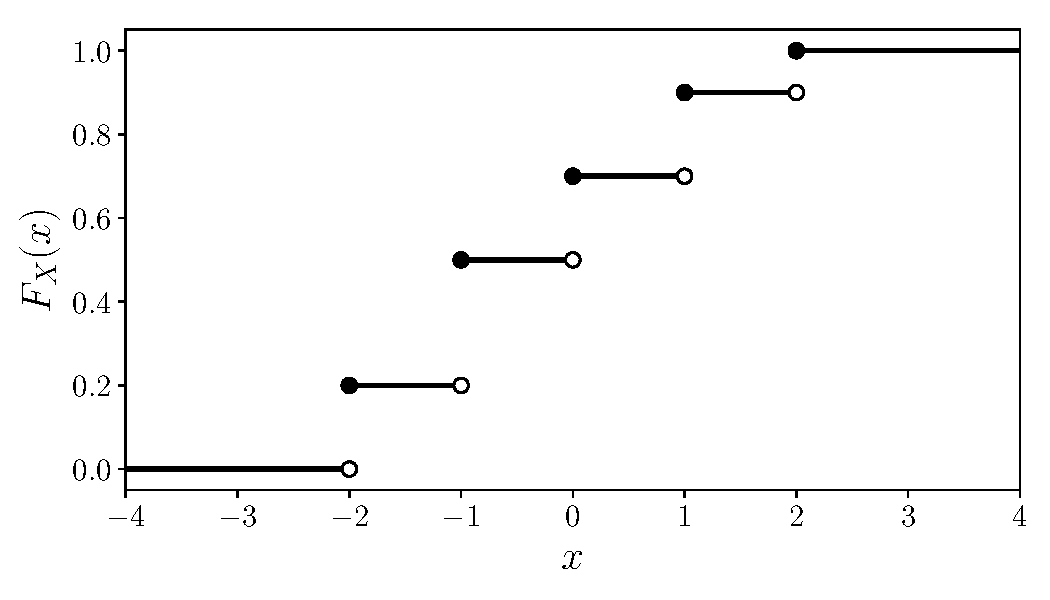
\includegraphics[totalheight=6cm]{chpt3/prob12.pdf}
  			  \caption{The associated CDF for the PMF of problem 12.}
    			   \label{fig:prob_12}
	\end{figure}

\end{problem}

\begin{problem}{13}  Whenever there is a jump in the CDF at a value of $x$, this indicates that that value of $x$ is in the range of $X$.  Therefore, $R_X=\{0, 1, 2, 3 \}$.  The probability at $x$ can be found by subtracting out the probabilities at values $<x$ from $F_X(x)$.  Therefore, the following equations give the probabilities we need:
\[
  \begin{cases}
                                   P(0)=F_X(0) \\
                                    P(1)=F_X(1)-P(0) \\
                                    P(2)=F_X(2)-P(1)-P(0) \\
                                    P(3)=F_X(3)-P(2)-P(1) -P(0),
  \end{cases}
\]
and when plugging in the values for $F_X(x)$, this leads to:
\[
  P_X(x) =
  \begin{cases}
                                   \frac{1}{6} & \text{for $x=0$} \\
                                   \frac{1}{3} & \text{for $x=1$} \\
                                   \frac{1}{4} & \text{for $x=2$} \\
                                   \frac{1}{4} & \text{for $x=3$}.
  \end{cases}
\]
As a sanity check, these probabilities do indeed add up to 1.



\end{problem}

\begin{problem}{14} $ $

\begin{enumerate}
\item
\begin{equation*}
E[X]  = 1\cdot 0.5+2\cdot 0.3+3\cdot 0.2 =1.7
\end{equation*}

\item 
\begin{equation*}
E[X^2] = 1\cdot 0.5+4\cdot 0.3+9\cdot 0.2 =3.5
\end{equation*}
$\implies$
\begin{equation*}
Var[X] = E[X^2]-E[X]^2 = 3.5-1.7^2=0.61
\end{equation*}
$\implies$
\begin{equation*}
SD[X] =\sqrt{Var[X]} \approx 0.78
\end{equation*}

\item Using LOTUS:

\begin{align*}
E[Y] & = \sum_{x \in R_X} \frac{2}{x} P_X(x) \\
& = \frac{2}{1}\cdot 0.5+\frac{2}{2}\cdot 0.3+\frac{2}{3}\cdot 0.2 \approx 1.43.
\end{align*}


\end{enumerate}

\end{problem}

\begin{problem}{15} The range of X is $\{1, 2, 3, \ldots \}$.  For $x\ge 5$, these values get mapped to $0, 1, 2, \ldots$.  The values $x=1, 2, 3, 4$ get mapped to $4, 3, 2, 1$, and thus $R_Y=\{0, 1, 2, \ldots\}$.  To solve for the the corresponding PMF, note that $P(X=k) = (1/3)(2/3)^{k-1}$, and that $P_Y(y=k)=P(Y=k)=P(|X-5|=k)$.  We therefore have:


  \begin{align*}
                                   P_Y(y=0) &= P(X=5) = \frac{1}{3}\left( \frac{2}{3}\right)^{4} \\
                                   P_Y(y=1) &= P(X=4~ \mathrm{or}~ X=6) =   \frac{1}{3} \left(\frac{2}{3}\right)^{3}+ \frac{1}{3}\left( \frac{2}{3}\right)^{5} \\
                                  P_Y(y=2) &= P(X=3~ \mathrm{or}~ X=7) =   \frac{1}{3} \left(\frac{2}{3}\right)^{2}+ \frac{1}{3}\left( \frac{2}{3}\right)^{6} \\
                                   P_Y(y=3) &=P(X=2~ \mathrm{or}~ X=8) =  \frac{1}{3}\left(\frac{2}{3}\right)^{1}+ \frac{1}{3} \left(\frac{2}{3}\right)^{7}   \\
                                   P_Y(y=4) &=P(X=1~ \mathrm{or}~ X=9) =   \frac{1}{3}\left( \frac{2}{3}\right)^{0}+ \frac{1}{3}\left( \frac{2}{3}\right)^{8} \\ 
                                   P_Y(y=5) &= P(X=10) =  \frac{1}{3}\left( \frac{2}{3}\right)^{9} \\
                                   P_Y(y=6) &= P(X=11) =  \frac{1}{3} \left(\frac{2}{3}\right)^{10} \\
                                  & \vdots 
  \end{align*}
One can easily check that this distribution is normalized by summing all terms on the RHS of the equations: $(1/3)\sum_{k=0}^{\infty}(2/3)^k =1$, where I have summed the geometric series.

\end{problem}

\begin{problem}{16} I first note that the range of $Y$ is $\{0, 1, 2, 3, 4, 5\}$, so that its PMF is

  \begin{align*}
                                   P_Y(y=0) &= P(X=-10~ \mathrm{or}~ X=-9~ \mathrm{or} \ldots ~ \mathrm{or}~ X=0) = \frac{11}{21} \\
                                   P_Y(y=1) &=P(X=1)  =  \frac{1}{21} \\
                                  P_Y(y=2) &= P(X=2) =   \frac{1}{21} \\
                                   P_Y(y=3) &=P(X=3) = \frac{1}{21}   \\
                                   P_Y(y=4) &=P(X=4) =   \frac{1}{21} \\ 
                                   P_Y(y=5) &= P(X=5~ \mathrm{or}~ X=6~ \mathrm{or} \ldots ~ \mathrm{or}~ X=10) =  \frac{6}{21},
  \end{align*}
which indeed sums to 1.

\end{problem}

\begin{problem}{17}  Since $E[X]$ was found to be $1/p$ for the geometric distribution from Example 3.12 in the book, if we can solve for $E[X^2]$ then we can compute the variance with $Var[X] = E[X^2]-E[X]^2$.  To do this, we will need a few formulas involving the geometric series.  I claim that:

\begin{equation*}
\sum_{k=0}^\infty x^k = \frac{1}{1-x} ~~~|x|<1,
\end{equation*}

\begin{equation*}
\sum_{k=0}^\infty k x^{k-1} = \frac{1}{(1-x)^2} ~~~|x|<1,
\end{equation*}
and
\begin{equation*}
\sum_{k=0}^\infty k^2 x^{k-1} =\frac{1+x}{(1-x)^3} ~~~|x|<1.
\end{equation*}
The first formula is simply the sum of a geometric series, the second was already proved in the book in Example 3.12.  I now prove the third formula.

\begin{proof}
We can take derivatives of the LHS and RHS of the second equation above to prove the third.  Differentiating the LHS results in:
\begin{align*}
\frac{d}{dx} \sum_{k=0}^\infty k x^{k-1} &= \sum_{k=0}^\infty k(k-1) x^{k-2} \\
& =  \sum_{k=1}^\infty k^2 x^{k-2}- \sum_{k=1}^\infty k x^{k-2} \\
& =\sum_{j=0}^\infty (j+1)^2 x^{j-1}- \sum_{k=0}^\infty (j+1) x^{j-1} \\
& =\sum_{j=0}^\infty j^2 x^{j-1}+2\sum_{j=0}^\infty j x^{j-1} +\sum_{j=0}^\infty x^{j-1}-\sum_{j=0}^\infty j x^{j-1}-\sum_{j=0}^\infty x^{j-1}\\
& = \sum_{j=0}^\infty j^2 x^{j-1}+\sum_{j=0}^\infty j x^{j-1} \\
&=\sum_{j=0}^\infty j^2 x^{j-1}+\frac{1}{(1-x)^2},
\end{align*}
where I have made the substitution $j=k-1$.  Differentiating the RHS results in:
\begin{equation*}
\frac{d}{dx} \frac{1}{(1-x)^2} = \frac{2}{(1-x)^3},
\end{equation*}
and putting the two together completes the proof.
\end{proof}
I may now solve for $E[X^2]$
\begin{align*}
E[X^2]&=\sum_{k=1}^\infty x^2p(1-p)^{k-1} \\
& = p\sum_{k=0}^\infty x^2(1-p)^{k-1} \\
& =\frac{p[1+(1-p)]}{[1-(1-p)]^3} \\
& = \frac{2-p}{p^2},
\end{align*}
so that the variance is:
\begin{equation*}
Var[X] = \frac{2-p}{p^2} -\frac{1}{p^2} = \frac{1-p}{p^2}.
\end{equation*}



\end{problem}


\begin{problem}{18}   In Problem 5 from 3.1.6 of the book, we showed that if $X_1, X_2, \ldots, X_m \sim Geom(p)=Pascal(1, p)$ (iid), then $X=X_1+X_2+ \ldots +X_m \sim Pascal(m, p)$.  Therefore $Var[X] = Var[X_1]+Var[X_2]+\ldots+Var[X_m] = m(1-p)/(p^2)$, by linearity in variance of independent random variables. 



\end{problem}

\begin{problem}{19}  I use LOTUS repeatedly in this problem and linearity of expectation.
\begin{align*}
E[X] &= E \left[ -\frac{Y}{2}+\frac{3}{2} \right] \\
& = -\frac{1}{2}E[Y]+\frac{3}{2} \\
& = 1
\end{align*}



\begin{align*}
Var[X] &= E[X^2]-E[X]^2 \\
& = E\left[\frac{Y^2}{4}-\frac{3Y}{2}+\frac{9}{4}\right] -1\\
&=\frac{1}{4}E[Y^2]-\frac{3}{2}E[Y]+\frac{9}{4}-1 \\
&=\frac{9}{4}-\frac{3}{2}+\frac{9}{4}-1 \\
&=2
\end{align*}

\end{problem}

\begin{problem}{20} $ $

\begin{enumerate}

\item
The range of $X$ is $\{1, 2, 3, 4, 5, 6\}$ and the probability for any of these values, $x$, is simply $N_x/1000$, where $N_x$ is the number of households with $x$ people.  Therefore: 
\[
  P_X(x) =
  \begin{cases}
                                   0.1 & \text{for $x=1$} \\
                                   0.2 & \text{for $x=2$} \\
                                  0.3 & \text{for $x=3$} \\
                                   0.2 & \text{for $x=4$} \\
                                  0.1 & \text{for $x=5$} \\
                                  0.1 & \text{for $x=6$}.
  \end{cases}
\]
The expected value of $X$ is: $E[X] = 1\cdot 0.1+2\cdot 0.2+3\cdot 0.3+4\cdot 0.2+5\cdot 0.1+6\cdot 0.1 =3.3$.


\item The probability of picking a person from a household with $k$ people is equal to the total number of people in households with $k$ people divided by the total number of people in the town.  In other words, $P(Y=k)=(k\cdot N_k)/3300$, so that:
\[
  P_Y(y) =
  \begin{cases}
                                   \frac{1}{33} & \text{for $y=1$} \\
                                   \frac{4}{33} & \text{for $y=2$} \\
                                  \frac{9}{33} & \text{for $y=3$} \\
                                   \frac{8}{33} & \text{for $y=4$} \\
                                  \frac{5}{33} & \text{for $y=5$} \\
                                  \frac{6}{33} & \text{for $y=6$},
  \end{cases}
\]
and $E[Y] = 1\cdot (1/33)+2 \cdot (4/33)+3\cdot (9/33)+4\cdot (8/33)+5\cdot (5/33)+6\cdot (6/33) =43/11$.

\end{enumerate}

\end{problem}

\begin{problem}{21} $ $

\begin{enumerate}
\item It takes 1 try to observe the first unique coupon.  Let this first coupon be called type $C_1$.  Let the random variable, $X_1$, be the number of times it takes to observe a coupon different than type $C_1$.  Call this type $C_2$.  Let the random variable, $X_2$, be the number of times it takes to observe a coupon different than type $C_1$ and $C_2$.  Call this type $C_3$.  Let us proceed in this fashion until we observe $N-1$ unique coupons.  Finally, let the random variable $X_{N-1}$ be the number of times it takes to observe a coupon different than type $C_1, C_2, \ldots, C_{N-1}$, and call this coupon type $C_N$.  Therefore, the total number of times it takes to observe all unique coupons at least once is $X=1+X_1+X_2+\ldots+X_{N-1}$.

For each $X_i$, if we consider choosing $C_1, C_2, \ldots$ or, $C_{i-1}$ as a failure and $C_{i}$ as a success, we see that this is nothing more than a geometric random variable with probability $(N-i)/N$ of success (since there are $N-i$ un-observed coupons left).  Therefore, $X_1, X_2, \ldots, X_{N-1} \sim Geom(\frac{N-i}{N})$.  Further let $X_0 \sim Geom(\frac{N-0}{N})$, and note that the probability of observing $X_0=1$ for this distribution is unity since we are sure to have a success on the first trial.  Thus, if we desire, we can replace 1 in $X=1+X_1+X_2+\ldots+X_{N-1}$ with the ``random variable" $X_0$.

\item
The expected number of tries it takes to observe all unique coupons at least once is:
\begin{align*}
E[X]&=E[1+X_1+X_2+\ldots+X_{N-1}]\\
&=1+E[X_1]+E[X_2]+\ldots+E[X_{N-1}]\\
& = 1+ \frac{N}{N-1}+\frac{N}{N-2}+\ldots+\frac{N}{N-(N-1)} \\
& = N\sum_{i=0}^{N-1}\frac{1}{N-i}.
\end{align*}
The summation can be written in terms of a special function (called the digamma function), but I believe it is more illustrative to plot the actual function itself.  In Fig.~\ref{fig:prob_21}, I show $E[X]$ for $N=1$ to 50 which I calculated numerically with the summation formula I derived above.

	\begin{figure}[t]
	\centering
      		 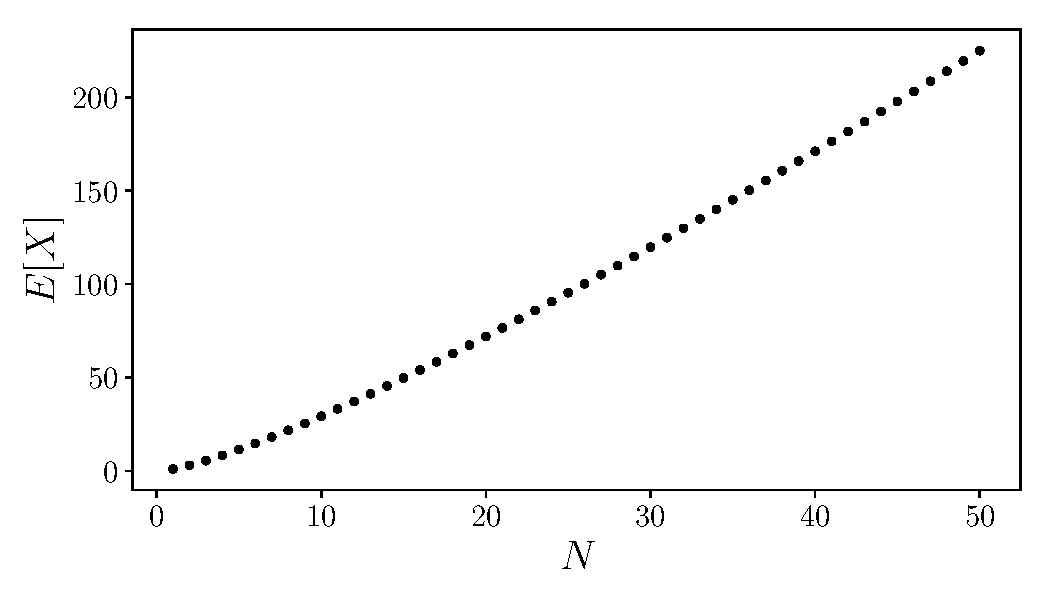
\includegraphics[totalheight=6cm]{chpt3/prob21.pdf}
  			  \caption{The expected number of tries to observe all unique coupons at least once.}
    			   \label{fig:prob_21}
	\end{figure}



\end{enumerate}

\end{problem}

\begin{problem}{22} $ $
\begin{enumerate}

\item Let $X^\prime$ be the number of tosses until the game ends.  We recognize that $X^\prime$ is distributed as a geometric random variable with $p=q=1/2$ since the coin is fair.   The range of $X^\prime$ is $R_{X^{\prime}}=\{1, 2, 3, 4 \ldots\}$.  Let the random variable $X$ denote the amount of money won from the game which has range $R_{X}=\{1, 2, 4, 8 \ldots\}$.  The function $f:R_{X^{\prime}}\rightarrow R_{X}$ is given by the bijective mapping $2^{X^{\prime}-1}$.  Thus, the PMF of $X$ is given by $P(X=x) = P(X^\prime=x^{\prime})$, where $x^\prime$ is the pre-image of $x$ under $f$.  That is, the PMF of $X$ is given by: $P(X=1) =P(X^\prime=1)=p$, $P(X=2) =P(X^\prime=2)=p^2$, $P(X=4) =P(X^\prime=3)=p^3$, $P(X=8) =P(X^\prime=4)=p^4, \ldots$.  Thus the expected value of $X$ is given by the following summation, which we see diverges:
\begin{align*}
E[X]& = \sum_{x \in R_X}xP(X=x) =\sum_{k=1}^\infty 2^{k-1}P(X^\prime=k) \\
& = \sum_{k=1}^\infty 2^{k-1} \left( \frac{1}{2} \right) \left(\frac{1}{2}\right)^{k-1} \\
& = \infty.
\end{align*}
Thus, only considering your expected winnings (and ignoring issues like the variance of your winnings and your particular risk tolerance) you would be willing to pay any amount of money to play this game.

\item By noting that $\ldots, 2^{6-1}, 2^{7-1}, 2^{8-1} \ldots = \ldots, 32, 64, 128, \ldots$, one sees that when $X^\prime=8$, $X=2^7 =128$ which is the first time that $X$ takes on a value greater than 65.  Therefore, the probability we desire is:
\begin{align*}
P(X>65) &= \sum_{k=8}^\infty P(X^\prime=k) \\
& = 1- \sum_{k=1}^7 \left(\frac{1}{2}\right)\left(\frac{1}{2}\right)^{k-1} \\
& = 1-\left[\left(\frac{1}{2}\right)^1+\left(\frac{1}{2}\right)^2+\ldots+\left(\frac{1}{2}\right)^7\right] \\
& = \frac{1}{128}.
\end{align*}

\item

This problem is very similar to part a, except that the summation is truncated when $x$ takes on the value $2^{30}$, which occurs when $k=31$, thereafter, the payout remains $2^{30}$.  Therefore, the expected value of $Y$ is:

\begin{align*}
E[Y]&=\sum_{k=1}^{31}2^{k-1}P(X^\prime=k)+\sum_{k=32}^{\infty}2^{30}P(X^\prime=k)\\
& = \sum_{k=1}^{31}\frac{1}{2}+2^{30}\sum_{k=32}^{\infty}\left(\frac{1}{2}\right)^k\\
& = \frac{31}{2}+2^{30}2^{-32}\sum_{k^\prime=0}^{\infty}\left(\frac{1}{2}\right)^{k^\prime}\\
& =  \frac{31}{2}+2^{30}2^{-32}\frac{1}{1-1/2} \\
& = 16.
\end{align*}
We therefore see that in part a, the majority of the summation that contributes to the expectation value of $X$ occurs much later in the series.  This is called a ``paradox" since, in the first part the expectation value was infinite, but in the second part, even though $2^{30}$ is a very large number, the expected winnings is much lower than what one would have guessed.


\end{enumerate}

\end{problem}


\begin{problem}{23}  The goal is to find:

\begin{equation*}
\alpha^{*}= \argmin_{\alpha \in \mathbb R} f(\alpha),
\end{equation*}
where
\begin{align*}
f(\alpha) &= E[(X-\alpha)^2] \\
&=E[X^2-2\alpha X+\alpha^2] \\
&=E[X^2]-2 \alpha \mu +\alpha^2.
\end{align*}
Therefore:
\begin{equation*}
\alpha^{*}= \argmin_{\alpha \in \mathbb R} \{ E[X^2]-2 \alpha \mu +\alpha^2 \} = \argmin_{\alpha \in \mathbb R} \{-2 \alpha \mu +\alpha^2\}, 
\end{equation*}
which we can be found by setting the derivative of this equation,
\begin{equation*}
\frac{d}{d \alpha} (-2 \alpha \mu +\alpha^2) = -2\mu+2\alpha,
\end{equation*}
equal to zero, and solving for $\alpha^{*}$.  This results in $\alpha^* = \mu$.



\end{problem}

\begin{problem}{24}  If you choose to roll the die for a second time, your expected winnings is $E[Y] = 3.5$.  Therefore, if you roll less than 3.5 on the first roll (i.e., 1, 2 or 3) you should roll again because you expect to do better on the second roll.  However, if you roll a 4, 5 or 6, you will expect to do worse on the second roll, so you should not roll again.

Given this strategy, your expected winnings is:

\begin{align*}
E[W] &= E[X \mathbbm 1\{ X>3\}]+E[Y \mathbbm 1\{ X \le 3\}] \\
& = E[X \mathbbm 1\{ X>3\}]+E[Y]E[ \mathbbm 1\{ X \le 3\}] \\
& = \frac{1}{6}\sum_{x=1}^6 x \mathbbm 1\{ x>3\}+\left(\frac{7}{2}\right) \left(\frac{1}{6}\right)\sum_{x=1}^6 \mathbbm 1\{ X \ge 3 \} \\
& = \frac{1}{6} (4+5+6)+\left(\frac{7}{2}\right) \left(\frac{1}{6}\right) (1+1+1) \\
&= \frac{17}{4} \\
&= 4.25,
\end{align*}
where, in the second equality, $E[Y \mathbbm 1\{ X \le 3\}]  = E[Y]E[ \mathbbm 1\{ X \le 3\}] $ since $X$ and $Y$ are independent (given the set strategy).  

\end{problem}

\begin{problem}{25} $ $

\begin{enumerate}
\item In Fig.~\ref{fig:prob_25} I have plotted both $P(X \ge x)$ and $P(X \le x)$ for this PMF.  It is clear from this figure that in the range $[2, \infty)$, $P(X \le x) \ge 1/2$, and that in the range $(-\infty, 2]$ $P(X \ge x) \ge 1/2$.  The only value that these ranges share in common is 2, and this is therefore the median for this PMF.

	\begin{figure}[t]
	\centering
      		 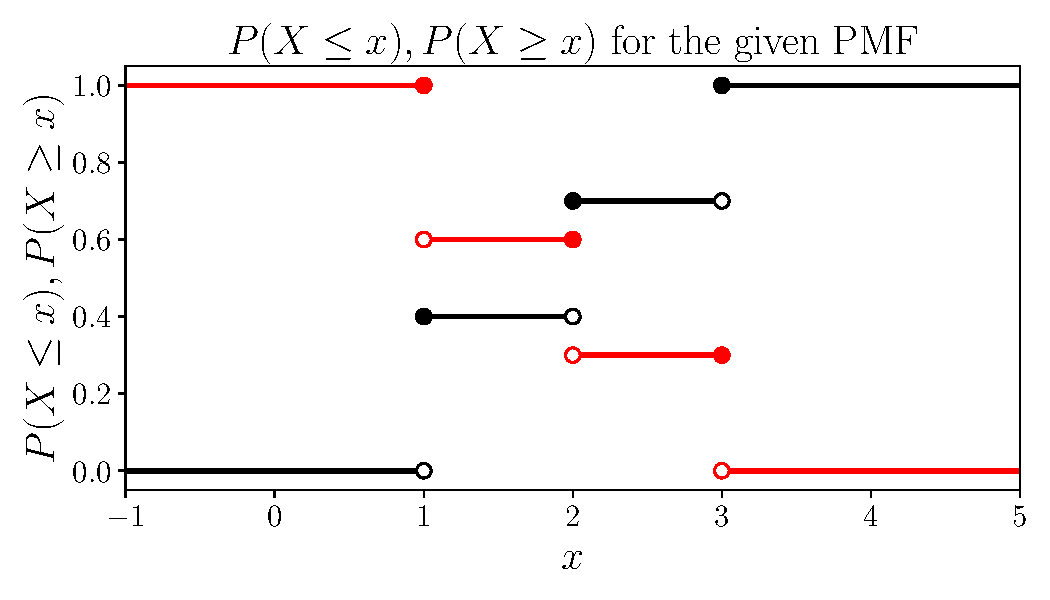
\includegraphics[totalheight=6cm]{chpt3/prob25.pdf}
  			  \caption{$P(X \ge x)$ (red) and $P(X \le x)$ (black) for Problem 25a.}
    			   \label{fig:prob_25}
	\end{figure}
	
\item In Fig.~\ref{fig:prob_25b} I have plotted both $P(X \ge x)$ and $P(X \le x)$ for a die roll.  It is clear from this figure that in the range $[3, \infty)$, $P(X \le x) \ge 1/2$, and that in the range $(-\infty, 4]$ $P(X \ge x) \ge 1/2$.  The (not unique) medians for this distribution are the intersection of these 2 sets, which is the interval $[3, 4]$.

	\begin{figure}[t]
	\centering
      		 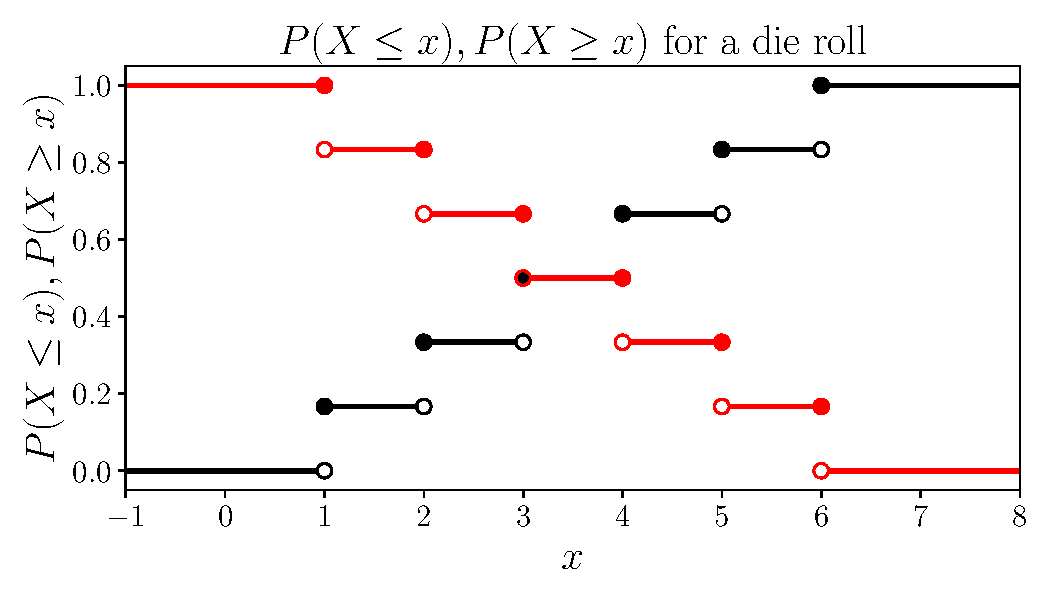
\includegraphics[totalheight=6cm]{chpt3/prob25b.pdf}
  			  \caption{$P(X \ge x)$ (red) and $P(X \le x)$ (black) for Problem 25b.}
    			   \label{fig:prob_25b}
	\end{figure}
	
	\item We can compute $P(X \le x)$ with the geometric distribution explicitly with:
	\begin{equation*}
	P(X \le x) = p \sum_{k=1}^{k^{u}_x}q^{k-1},
	\end{equation*}
where $q=1-p$ and $k^{u}_x$ is the appropriate upper integer bound which depends on the (not necessarily integer) value of $x$.  By considering the staircase shape of $P(X \le x)$, one can realize that for any $x$, $P(X \le x) = P(X \le \floor{x})$, which holds up until $\ceil{x}$ (where $\floor{\cdot}$ and $\ceil{\cdot}$ are defined as rounding down and up to the nearest integer respectively).  Therefore, if we want to find the lowest value of $x$, $x^\prime$ for $P(X \le x^\prime)$ still equals $P(X \le x)$, this occurs at the integer value $x^\prime= \floor{x}$.  $\floor{x}$ is therefore the appropriate value to use for ${k^{u}_x}$, and we can explicitly compute a formula for $P(X \le x)$:
\begin{align*}
P(X \le x) & = P(X \le \floor{x}) \\
&= pq^{-1} \sum_{k=1}^{\floor{x}}q^{k}\\
& = pq^{-1} \left[-q^0+\sum_{k=0}^{\floor{x}}q^{k} \right] \\
& = pq^{-1}\left [-1 +\sum_{k=0}^{\infty}q^{k} -\sum_{k=\floor{m}+1}^{\infty}q^{k} \right] \\
& =  pq^{-1}\left [-1 +\sum_{k=0}^{\infty}q^{k} -q^{\floor{x}+1}\sum_{k^\prime = 0}^{\infty}q^{k^\prime} \right] \\
& = pq^{-1}\left [-1 +\frac{1}{1-q} -\frac{q^{\floor{x}+1}}{1-q} \right] \\
& = 1-q^{\floor{x}}.
\end{align*}
Any value $m$, for which $P(X \le m) \ge 1/2$ is a potential candidate for the median (but of course we still have to consider the values of $x$ for which $P(X \ge x) \ge 1/2$) and the lowest value for which this occurs, call it $\floor{m_L}$, can now be found by setting $P(X \le \floor{m_L}) = 1/2$, resulting in:
\begin{equation*}
\floor{m_L} = \frac{1}{\log_2{1/q}}.
\end{equation*}
Similarly:
\begin{align*}
P(X \ge x) & =P(X \ge \ceil{x}) \\
&= pq^{-1} \sum_{k=\ceil{x}}^{\infty}q^{k}\\
& = pq^{\ceil{x}-1} \sum_{k^\prime = 0}^{\infty}q^{k^\prime} \\
& = \frac{ pq^{\ceil{x}-1} }{1-q} \\
& =q^{\ceil{x}-1}.
\end{align*}
Thus, the highest value for which $P(X \ge x) \ge 1/2$, call it $\ceil{m_U}$ is found when this equation equals 1/2, resulting in:
\begin{equation*}
\ceil{m_U} = \frac{1}{\log_2{1/q}}+1.
\end{equation*}
Therefore, for the geometric distribution, $P(X \le m) \ge 1/2$ and $P(X \ge m) \ge 1/2$ for $x\in \left [\floor{m_L}, \ceil{m_U} \right]$.  This interval thus gives the (not unique) medians for the geometric distribution.

	

	
\end{enumerate}

\end{problem}





\chapter{Continuous and Mixed Random Variables}
\begin{problem}{1}  $ $
\begin{enumerate}
\item
We recognize that this is a uniform random variable, so its CDF is:
\[
  F_X(x) =
  \begin{cases}
                                   0 & \text{for $x < 2$} \\
                                   \frac{x-2}{4} & \text{for $2 \le x \le 6$} \\
 1 & \text{for $x>6$}.
  \end{cases}
\]

\item
For a uniform random variable, the expectation value is at the midpoint: $E[X] = 2+[(6-2)]/2 = 4$.


\end{enumerate}
\end{problem}

\begin{problem}{2}  $ $
\begin{enumerate}

\item By normalization, $1 = c \int_0^\infty \exp{(-4x)}dx$, which leads to $c=4$. 

\item
\begin{equation*}  
  F_X(x) = \begin{cases}
                                   0 & \text{for $~x \le 0$} \\
                                   4\int_0^x e^{-4 x^\prime dx^\prime} & \text{for  $x>0$} 
       \end{cases} \quad
= \begin{cases}
                                   0 & \text{for $~x \le 0$} \\
                                   1 - e^{-4 x} & \text{for  $x>0$}.
       \end{cases}
\end{equation*}

\item

\begin{equation*}
P(2 < X < 5) = 4 \int_2^5 e^{-4x}dx = e^{-8}-e^{-20}.
\end{equation*}

\item
To find the expectation value, I use integration by parts:

\begin{align*}
E[X] &= 4\int_0^\infty x e^{-4x}dx \\
& = -\left(x e^{-4x} \right)_0^\infty +\int_0^\infty e^{-4x}dx \\
& = \frac{1}{4},
\end{align*}

where the limits in the first term were evaluated using L'hopital's rule.

\end{enumerate}
\end{problem}

\begin{problem}{3}  $ $
\begin{enumerate}

\item
Using LOTUS:
\begin{align*}
E\left[X^n\left(X^2+\frac{2}{3}\right)\right] &= \int_0^1 x^n\left(x^2+\frac{2}{3}\right)dx \\
& = \frac{1}{3+n}x^{3+n} \Big|_0^1 +\left(\frac{2}{3}\right)\frac{1}{n+1}x^{n+1} \Big|_0^1 \\
& = \frac{1}{3+n}+\left(\frac{2}{3}\right)\frac{1}{n+1}~~\mathrm{for}~n=1, 2, 3, \ldots
\end{align*}

\item
We have already found $E[X]$ and $E[X^2]$ in the first part and thus:
\begin{align*}
Var[X] & = E[X^2]- E[X]^2 \\
& = \frac{1}{3+2}+\left(\frac{2}{3} \right)\frac{1}{2+1}- \left [ \frac{1}{3+1}+\left(\frac{2}{3} \right)\frac{1}{1+1} \right]^2 \\
& = \frac{59}{720}.
\end{align*}
\end{enumerate}
\end{problem}


\begin{problem}{4} $ $
\begin{enumerate}
\item For this problem, we have $R_X = [0, 1]$ and $R_Y = [1/e, 1]$.  Thus in range of $x=$ 0 to 1, the CDF of $Y$ is given by:

\begin{align*}
F_Y(y) & = P(Y \le y) \\
& = P(e^{-X} \le y ) \\
& = P(X \ge -\ln{y} ) \\
& = 1-F_X(-\ln{y} ) \\
& = 1+\ln y,
\end{align*}
where I used the fact that for $x \in [0, 1]$ for a uniform 0, 1 distribution, $F_X(x)=x$.
Therefore:
\[
  F_Y(y) =
  \begin{cases}
                                   0 & \text{for $y<\frac{1}{e}$} \\
                                   1+\ln(y) & \text{for $\frac{1}{e} \le y \le 1$} \\
                                   1 & \text{for $y>1$}.
  \end{cases}
\]

\item
\[
  f_Y(y) = \frac{ d F_Y}{dy}=
  \begin{cases}
                                   0 & \text{for $y<\frac{1}{e}$} \\
                                   \frac{1}{y} & \text{for $\frac{1}{e} \le x \le 1$} \\
                                   0 & \text{for $x>1$}
  \end{cases}
\]

\item

\begin{equation*}
E[Y] = \int_{1/e}^1 y \frac{1}{y} dy = 1-\frac{1}{e}
\end{equation*}

\end{enumerate}

\end{problem}


\begin{problem}{5} $ $

\begin{enumerate}

\item The range of $X$ and $Y$ are $R_X = (0, 2]$ and $R_Y = (0, 4]$, so that for $y \in R_Y$, we have

\begin{align*}
F_Y(y) &= P(Y \le y)\\
& = P(X^2 \le y) \\
& = P(0  <X < \sqrt{y}) \\
& = \int_0^{\sqrt{y}} \frac{5}{32}x^4 dx \\
& = \frac{1}{32}y^{5/2},
\end{align*} 
and therefore:
\[
  F_Y(y) =
  \begin{cases}
                                   0 & \text{for $y \le 0$} \\
                                   \frac{1}{32}y^{5/2} & \text{for $0<y \le 4$} \\
                                   1 & \text{for $y>4$}.
  \end{cases}
\]

\item 
\[
  f_Y(y) = \frac{ d F_Y}{dy}=
  \begin{cases}
                                   0 & \text{for $y \le 0$} \\
                                  \frac{5}{64}y^{3/2} & \text{for $0<y \le 4$} \\
                                   0 & \text{for $y>4$}
  \end{cases}
\]
 
\item

\begin{equation*}
E[Y] = \frac{5}{64}\int_0^4 y\cdot y^{3/2} \approx 2.9
\end{equation*}
 
\end{enumerate}

\end{problem}





\begin{problem}{6}  We can convert the PDF for $X$ to the PDF for $Y$ using the method of transformations:


\[
  f_Y(y) = f_X\left(\frac{y}{\alpha}\right)\left|\frac{ d (y/\alpha)}{dy}\right|=
  \begin{cases}
                                   \frac{\lambda}{\alpha}e^{-\frac{\lambda}{\alpha} y} & \text{for $y>0$} \\
                                   0 & \text{otherwise} 

  \end{cases},
\]
and since both $\alpha, \lambda>0$, $Y\sim Exp(\lambda/\alpha)$.

\end{problem}

\begin{problem}{7} $ $

\begin{enumerate}
\item  We can prove this relation using integration by parts:

\begin{align*}
E[X^n] &= \int_0^\infty x^n \lambda e^{-\lambda x}dx \\
& = -x^n e^{-\lambda x}\Big|_0^\infty +\frac{n}{\lambda}\int_0^\infty x^{n-1} \lambda e^{\lambda x}dx \\
 & = \frac{n}{\lambda}E[X^{n-1}],
\end{align*}
where the first term evaluated to zero by repeated application of L'Hopital's rule.

\item We can use several properties of the Gamma function to prove this relation:

\begin{align*}
E[X^n] &= \int_0^\infty x^n \lambda e^{-\lambda x}dx \\
&=\frac{\lambda}{\lambda^{n+1}}\Gamma(n+1) \\
& = \frac{n!}{\lambda^n},
\end{align*}
where in the second equality I used the second property of the Gamma function given in the book, and in the third equality I used the fourth property of the Gamma function given in the book.

\end{enumerate}

\end{problem}

\begin{problem}{8} $ $

\begin{enumerate}
\item

\begin{equation*}
P(X>0) = 1- \Phi \left(\frac{0-3}{3} \right) \approx 0.84
\end{equation*}

\item

\begin{equation*}
P(-3<X<8) = \Phi \left(\frac{8-3}{3} \right)- \Phi \left(\frac{-3-3}{3} \right) \approx 0.93
\end{equation*}

\item

\begin{align*}
P(X>5|X>3) &=\frac{P(X>5, X>3)}{P(X>3)} \\
& = \frac{P(X>5)}{P(X>3)} \\
& = \frac{1-\Phi \left(\frac{5-3}{3} \right)}{1-\Phi \left(\frac{3-3}{3} \right)} \\
& \approx 0.50
\end{align*}


\end{enumerate}

\end{problem}

\begin{problem}{9} By Theorem 4.3 in the book, if $X \sim \mathcal N(3, 9)$, and $Y =5-X$, then $Y \sim \mathcal N(-3+5, 9)=\mathcal N(2, 9)$.

\begin{enumerate}
\item 

\begin{equation*}
P(X>2) = 1-\Phi \left(\frac{2-3}{3} \right) \approx 0.63
\end{equation*}

\item

\begin{equation*}
P(-1<Y<3) = \Phi \left(\frac{3-2}{3} \right) -\Phi \left(\frac{-1-2}{3} \right)  \approx 0.47
\end{equation*}

\item

\begin{align*}
P(X>4|Y<2) &=P(X>4|5-X<2) \\
&=\frac{P(X>4, X>3)}{P(X>3)} \\
& = \frac{P(X>4)}{P(X>3)} \\
& = \frac{1-\Phi \left(\frac{4-3}{3} \right)}{1-\Phi \left(\frac{3-3}{3} \right)} \\
& \approx 0.74
\end{align*}


\end{enumerate}

\end{problem}



\begin{problem}{10}  I first note that $R_X = \mathbb R$, and $R_Y=[0, \infty)$.  The range of $X$ can be partitioned into 2 regions, $X \le 0$ and $X>0$ which are strictly decreasing, and increasing respectively, where the corresponding inverse transformation back to $X$ for both of these regions is:
\[
X=
  \begin{cases}
                                   -Y^2 & \text{for $X \le 0$} \\
                                   Y^2 & \text{for $X>0$}.
  \end{cases}
\]
Therefore:
\begin{align*}
f_Y(y) &=f_X(y^2)\left|\frac{d(y^2)}{dy}\right|+f_X(-y^2) \left |\frac{d(-y^2)}{dy}\right |\\
& =\frac{4}{\sqrt{2 \pi}}y e^{-\frac{y^4}{2}} ~~~ \mathrm{for}~ y \ge 0,
\end{align*}
which, as a sanity check, I made sure analytically integrates to unity over the range 0 to infinity.



\end{problem}


\begin{problem}{11} $ $

\begin{enumerate}
\item

\begin{equation*}
P(X>2)  = 2 \int_2^{\infty}e^{-2 x} = e^{-4}
\end{equation*}

\item I calculate $E[Y]$ using LOTUS:

\begin{align*}
E[Y] &= \int_0^\infty (2+3x)2 e^{-2x}dx \\
 & = 2\int_0^\infty 2 e^{-2x}dx+3\int_0^\infty 2x e^{-2x}dx \\
 & = 2+3E[X]\\
 &=2+\frac{3}{2} \\
 & = \frac{7}{2},
\end{align*}
where I have used the fact that $E[X]$ for $Exp(\lambda)$ is $1/\lambda$ (as computed in the book).
To compute $Var[Y]$, I first must compute $E[Y^2]$, which I do using LOTUS:

\begin{align*}
E[Y^2] &= \int_0^\infty (2+3x)^22 e^{-2x}dx \\
 & = 4\int_0^\infty 2 e^{-2x}dx+12\int_0^\infty 2x e^{-2x}dx+9\int_0^\infty 2x^2 e^{-2x}dx \\
 & = 4+12E[X]+9E[X^2]\\
 &=4+\frac{12}{2}+\frac{9 \cdot 2}{4} \\
 & = \frac{29}{2},
\end{align*}
where I have used the fact that $E[X^2]$ for $Exp(\lambda)$ is $2/(\lambda^2)$ (as computed in the book).  Finally, the variance is:

\begin{equation*}
Var[Y] = E[Y^2]-E[Y]^2 = \frac{9}{4}.
\end{equation*}

\item

\begin{align*}
P(X>2|Y<11) &=P(X>2|2+3X<11) \\
&=P(X>2|X<3) \\
&=\frac{P(2<X<3)}{P(X<3)} \\
& = \frac{2 \int_2^3 e^{-2x}dx}{2 \int_0^3 e^{-2x}dx} \\
& = \frac{e^{2}-1}{e^{6}-1}\\
& \approx 1.6 \times 10^{-2}
\end{align*}


\end{enumerate}



\end{problem}



\begin{problem}{12} The equations defining the median for a continuous variable, $P(X<m) =1/2$ and $P(X \ge m) =1/2$,  are actually equivalent.  That is, $P(X<m) =1/2 \Leftrightarrow  P(X \ge m)=1/2$ (which can easily be verified), so we can use whichever is convenient.  Since we know the CDFs for the desired distributions, so using the condition that $P(X<m) =1/2$ will be most convenient.

\begin{enumerate}
\item  The CDF for the $Unif(a, b)$ is:

\[
  P(X < x) =
  \begin{cases}
                                   0 & \text{for $x < a$} \\
                                  \frac{x-a}{b-a} & \text{for $a\le x \le b$} \\
                                   1 & \text{for $x > b$},
  \end{cases}
\]
where I have ignored the equality in the argument of $P$, since $P(X = x)=0$ for a continuous random variable.  Setting this equation equal to $1/2$ and solving for $m$, I find:
\begin{equation*}
m = \frac{b+a}{2},
\end{equation*}
which is the mean of the uniform distribution, which was expected since the uniform distribution is symmetric about its mean.

\item The CDF for the $Exp(\lambda)$ is:

\[
P(Y<y) = 
  \begin{cases}
                                   0 & \text{for $y < 0$} \\
                                   1-e^{-\lambda y} & \text{for $y \ge 0$},
  \end{cases}
\]
where again, I have ignored the equality in the argument of $P$, since $P(Y = y)=0$.  Thus we see that $1/2 = 1- \exp{(-\lambda m)} \implies m = \ln{2}/\lambda$.

\item For the $\mathcal N(\mu, \sigma^2)$, 

\begin{align*}
P(W < m) &= P(W \le m) \\
& = \Phi \left (\frac{m-\mu}{\sigma} \right) \\
& = \frac{1}{2}.
\end{align*}
Since the standard normal is symmetric about 0, this implies that $\Phi(0) = 1/2$, and therefore $(m-\mu)/\sigma = 0$, and thus $m=\mu$.  Since we knew that a Gaussian is symmetric about its mean, this is what we expected.


\end{enumerate}

\end{problem}


\begin{problem}{13} $ $
\begin{enumerate}
\item See Fig.~\ref{fig:prob_13} for a plot of the CDF.  $X$ is a mixed random variable because there is a jump in the CDF at $x=1/4$ (indicating a probability ``point mass" at 1/4 of $P(X=1/4)=1/2$) and the CDF does not exhibit the staircase shape associated with only discrete random variables.

	\begin{figure}[t]
	\centering
      		 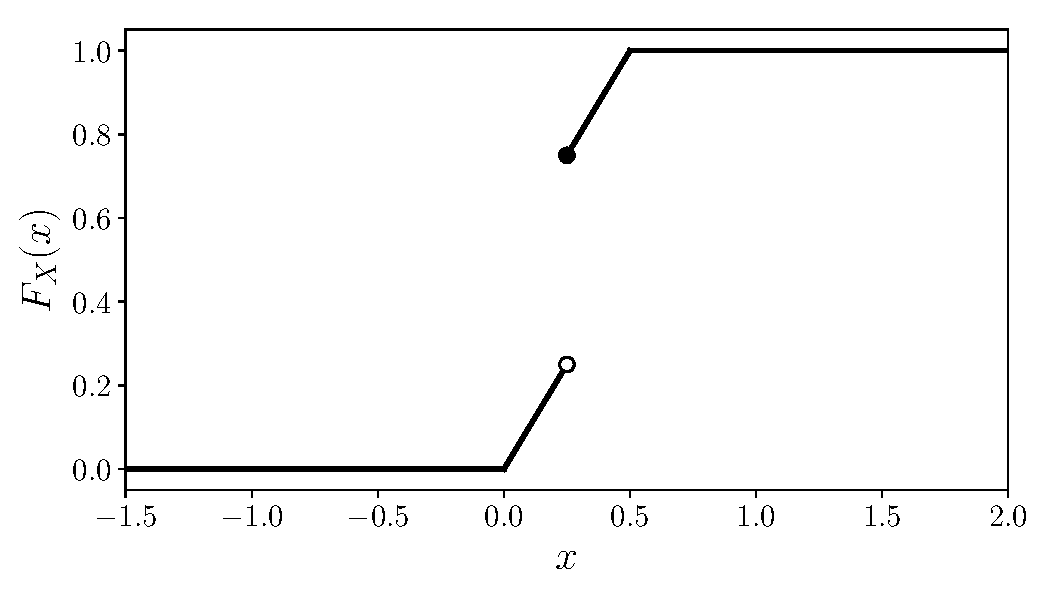
\includegraphics[totalheight=6cm]{chpt4/prob13.pdf}
  			  \caption{CDF for Problem 13}
    			   \label{fig:prob_13}
	\end{figure}

\item
\begin{align*}
P\left(X \le \frac{1}{3}\right) &= F_X\left(\frac{1}{3}\right) \\
&= \frac{1}{3} +\frac{1}{2}  \\
&= \frac{5}{6}
\end{align*}

\item 
\begin{align*}
P\left(X \ge \frac{1}{4}\right) &= 1 - P\left(X<\frac{1}{4}\right) \\
& = 1-\left[P\left(X \le \frac{1}{4}\right)-P\left(X=\frac{1}{4}\right)\right] \\
& = 1-\left[F_X\left(\frac{1}{4}\right)-P\left(X=\frac{1}{4}\right)\right] \\
& = 1-\left(\frac{1}{4}+\frac{1}{2}-\frac{1}{2}\right) \\
& = \frac{3}{4}
\end{align*}

\item

The CDFs for both the discrete and continuous contributions can be written piece-wise as:
\[
D(x) = 
  \begin{cases}
                                   0 & \text{for $x < \frac{1}{4}$} \\
                                   \frac{1}{2}& \text{for $x \ge \frac{1}{4}$},
  \end{cases}
\]
and
\[
C(x) = 
  \begin{cases}
                                   0 & \text{for $x < 0$} \\
                                   x & \text{for $\frac{1}{2} \le x \le \frac{1}{2}$} \\
                                   \frac{1}{2}& \text{for $x>\frac{1}{2}$}.
  \end{cases}
\]
These functions can be re-written using the unit step function:
\begin{equation*}
D(x) = \frac{1}{2}u\left(x-\frac{1}{4}\right),
\end{equation*}
and
\begin{equation*}
C(x) = xu(x) -  xu\left(x-\frac{1}{2}\right)+\frac{1}{2}u\left(x-\frac{1}{2}\right),
\end{equation*}
where, in $C(x)$, I have started subtracting off the linear equation at $x=1/2$, and adding a constant 1/2 at $x=1/2$ so as to keep the function flat at 1/2 after $x=1/2$.

\item
Since $C(x)$ increases linearly from 0 to 1/2, and has total probability mass 1/2, we expect $c(x)$ to be uniform with height 1 over the range 0 to 1/2.  Differentiating $C(x)$

\begin{align*}
c(x) & = \frac{d}{dx}C(x) \\
& = u(x) +x \frac{du(x)}{dx}-u\left(x-\frac{1}{2}\right)-x \frac{d}{dx}u\left(x-\frac{1}{2}\right)+\frac{1}{2}\frac{d}{dx}u\left(x-\frac{1}{2}\right) \\
& = u(x)+x\delta(x) - u \left (x-\frac{1}{2}\right)-x\delta \left(x-\frac{1}{2}\right)+\frac{1}{2}\delta \left(x-\frac{1}{2}\right) \\
& = u(x) -u\left(x-\frac{1}{2}\right),
\end{align*}
which is exactly what we had anticipated.  Here I used the fact that when $x \ne 1/2$, $x\delta(x-1/2)$ and $(-1/2)\delta(x-1/2)$ equal 0, while for for $x =1/2$, $(-1/2) \delta(x-1/2) = (-1/2)\delta(0)$ and $x \delta(x-1/2) = (1/2)\delta(0)$.  Also, in either case, $x \delta(x) = 0$.

\item

\begin{align*}
E[X] &= \int_{-\infty}^{\infty}x c(x) dx+\sum_{k}x_k a_k \\
& = \int_0^{1/2}x dx+\frac{1}{4}P\left(X=\frac{1}{4}\right) \\
& = \frac{1}{2}x^2\Big|_0^{1/2} dx+\frac{1}{4}\cdot \frac{1}{2} \\
& = \frac{1}{4}
\end{align*}

\end{enumerate}


\end{problem}


\begin{problem}{14}$ $


\begin{enumerate}
\item The generalized PDF of X is:
\begin{align*}
f_X(x) &= \frac{d}{dx}F_X(x) \\
& =   \frac{d}{dx}D(x)+\frac{d}{dx}C(x) \\
& = \frac{1}{2}\delta \left(x-\frac{1}{4}\right)+c(x) \\
& =  \frac{1}{2}\delta \left(x-\frac{1}{4}\right)+\left[u(x)-u\left(x-\frac{1}{2}\right)\right],
\end{align*}
where $c(x)$ was found in the previous problem.

\item
\begin{align*}
E[X] &= \frac{1}{2}\int_{-\infty}^{\infty}x\delta \left(x-\frac{1}{4}\right)dx + \int_{-\infty}^{\infty}xu(x)dx-\int_{-\infty}^{\infty}xu\left(x-\frac{1}{2}\right)dx \\
&= \frac{1}{2}\int_{-\infty}^{\infty}x\delta \left(x-\frac{1}{4}\right)dx + \int_0^{1/2}x dx\\
& = \frac{1}{2}\cdot\frac{1}{4}+\frac{1}{8} \\
& = \frac{1}{4}
\end{align*}


\item
\begin{align*}
E[X^2]&=\frac{1}{2}\int_{-\infty}^{\infty}x^2\delta \left(x-\frac{1}{4}\right)dx + \int_{0}^{1/2}x^2dx \\
& = \frac{1}{2} \left(\frac{1}{4} \right)^2+\frac{1}{3}x^3\Big|_0^{1/2} \\
& = \frac{7}{96}
\end{align*}
$\implies$
\begin{align*}
Var[X]&=E[X^2] - E[X]^2 \\
& =  \frac{7}{96} - \left(\frac{1}{4}\right)^2 \\
& = \frac{1}{96}
\end{align*}



\end{enumerate}

\end{problem}

\begin{problem}{15} $ $

\begin{enumerate}
\item

From the form of the given generalized PDF, it is clear that there are 2 probability point masses at $x=1$ and $x=-2$ (with $P(X=1)=1/6$ and $P(X=-2)=1/3$), as well as a continuous random variable contribution from a Gaussian PDF.  Since the continuous PDF contributes 0 probability at specific points, $P(X=1)=1/6$ and $P(X=-2)=1/3$.


\item

\begin{align*}
P(X \ge 1)& = \int_1^{\infty} \left [ \frac{1}{3}\delta(x+2) +\frac{1}{6}\delta(x-1)+\frac{1}{2}\frac{1}{\sqrt{2 \pi}}e^{-\frac{x^2}{2}} \right] dx \\
& = \frac{1}{6}+\frac{1}{2}\int_{1}^\infty  \frac{1}{\sqrt{2 \pi}}e^{-\frac{x^2}{2}}dx \\
& = \frac{1}{6}+\frac{1}{2} \left [ 1-\Phi(1) \right] \\
& \approx 0.25
\end{align*}

\item

\begin{align*}
P(X=1|X \ge 1) &= \frac{P(X=1, X \ge 1)}{P(X \ge 1)} \\
&= \frac{P(X=1)}{P(X \ge 1)} \\
&= \frac{\frac{1}{6}}{ \frac{1}{6}+\frac{1}{2} \left [ 1-\Phi(1) \right]} \\
& \approx 0.68
\end{align*}

\item We can calculate $E[X]$ by explicitly integrating over the generalized PDF:
\begin{align*}
E[X] & = \int_{-\infty}^{\infty} x \left [ \frac{1}{3}\delta(x+2) +\frac{1}{6}\delta(x-1)+\frac{1}{2}\frac{1}{\sqrt{2 \pi}}e^{-\frac{x^2}{2}} \right] dx\\
& = \frac{1}{3}(-2)+\frac{1}{6}(1)+\frac{1}{2}\int_{-\infty}^{\infty} x \frac{1}{\sqrt{2 \pi}}e^{-\frac{x^2}{2}} dx \\
& = \frac{-2}{3} +\frac{1}{6}+\frac{1}{2}\cdot 0 \\
& = -\frac{1}{2},
\end{align*}
where the integral in the second line is equal to zero, since this is just the mean of a standard normal distribution.

We can also calculate $E[X^2]$ by explicitly integrating over the generalized PDF:
\begin{align*}
E[X^2] & = \int_{-\infty}^{\infty} x^2 \left [ \frac{1}{3}\delta(x+2) +\frac{1}{6}\delta(x-1)+\frac{1}{2}\frac{1}{\sqrt{2 \pi}}e^{-\frac{x^2}{2}} \right] dx\\
& = \frac{1}{3}(4)+\frac{1}{6}(1)+\frac{1}{2}\int_{-\infty}^{\infty} x^2 \frac{1}{\sqrt{2 \pi}}e^{-\frac{x^2}{2}} dx \\
& = \frac{4}{3} +\frac{1}{6}+\frac{1}{2}(1) \\
& =2,
\end{align*}
where the integral in the second line is equal to 1, since this is just the variance of a standard normal distribution.

Thus:
\begin{align*}
Var[X]&=E[X^2] - E[X]^2 \\
& = 2 - \left(-\frac{1}{2}\right)^2 \\
& = \frac{7}{4}.
\end{align*}

\end{enumerate}



\end{problem}


\begin{problem}{16} $ $

\begin{enumerate}
\item Let $D$ denote the event that the device is defective, and let $P(D) = p_d = 0.02$.  By the law of total probability, we have:

\begin{align*}
F_X(x) &= P(X \le x) \\
&= P(X \le x|D)P(D)+ P(X \le x|D^c)P(D^c)\\
&= u(x)p_d+(1-e^{-\lambda x})(1-p_d)u(x).
\end{align*}

By differentiating, we can find the generalized PDF:
\begin{align*}
f_X(x) &= \frac{d}{dx} F_X(x) \\
&= p_d \delta(x) +(1-p_d)\left[(1-e^{-\lambda x}) \delta(x) +u(x) \lambda e^{-\lambda x} \right] \\
& =p_d \delta(x) +(1-p_d)u(x) \lambda e^{-\lambda x},
\end{align*}
where I have used the fact that at $x \ne 0$, $\delta(x)=0$, and at $x=0$, $(1-\exp{(-\lambda x)})=0$, so that the term, $(1-e^{-\lambda x}) \delta(x)$ is 0 for all $x$.  We also could have written this PDF down immediately by realizing that there is a probability point mass at $x=0$ with total probability $0.02$, and there is a continuous probability contribution from the exponential distribution which must integrate to $1-0.02=0.98$.

\item

\begin{align*}
P(X \ge 1) &= \int_1^{\infty}\left [p_d \delta(x)+(1-p_d)u(x)\lambda e^{-\lambda x} \right] dx \\
& = (1-p_d)\int_1^{\infty}\lambda e^{-\lambda x}dx \\
& = (1-p_d)e^{-\lambda} \\
& = (0.98)e^{-2} \\
& \approx 0.133
\end{align*}

\item
\begin{align*}
P(X >2| X \ge 1) &= \frac{P(X >2,X\ge 1) }{P(X \ge 1) }  \\
&= \frac{P(X >2) }{P(X \ge 1) } \\
&= \frac{\int_2^{\infty}e^{-\lambda x}dx}{\int_1^{\infty}e^{-\lambda x}dx} \\
& = e^{-\lambda} \\
& = e^{-2} \\
& \approx 0.135
\end{align*}

\item
The expectation value of $X$ is:
\begin{align*}
E[X] &= \int_{-\infty}^{\infty}x\left [p_d \delta(x)+(1-p_d)u(x)\lambda e^{-\lambda x} \right] dx \\
&= (1-p_d)\int_0^{\infty}x\lambda e^{-\lambda x}dx \\
&= (1-p_d)\frac{1}{\lambda} \\
&= (0.98)\frac{1}{2} \\
&=0.49,
\end{align*}
where I have used the fact that $E[X] = 1/\lambda$ for an exponential distribution.

The expectation value of $X^2$ is:
\begin{align*}
E[X^2] &= \int_0^{\infty}x^2\left [p_d \delta(x)+(1-p_d)u(x)\lambda e^{-\lambda x} \right] dx \\
&= (1-p_d)\int_0^{\infty}x^2\lambda e^{-\lambda x}dx \\
&= (1-p_d)\frac{2}{\lambda^2} \\
&= (0.98)\frac{1}{2} \\
&=0.49,
\end{align*}
where I have used the fact that $E[X^2] = 2/\lambda^2$ for an exponential distribution.  Therefore, the variance is:
\begin{align*}
Var[X]&=0.49 - 0.49^2 \\
& \approx 0.25.
\end{align*}
\end{enumerate}
\end{problem}

\begin{problem}{17} $ $

\begin{enumerate}
\item
We realize that for $Lap(0, 1)$, $f_X(x)$ is an even function, while $x$ is an odd function and therefore $E[X]=0$.  Also, 
\begin{align*}
E[X^2] = 2\int_0^{\infty}x^2\frac{1}{2}e^{-x}dx
&=2,
\end{align*}
where I have used the fact that since we are integrating an even function times an even function we need only integrate from $0$ to $\infty$ and multiply by 2.  I have also used the fact that the integrand is $E[X^2]$ of an $Exp(1)$ distribution, and we know this integral evaluates to $2/\lambda^2$.  Therefore $Var[X] = 2$.

\item We can solve for $f_Y(y)$ using the method of transformations:

\begin{align*}  
  f_Y(y) &= f_X\left(\frac{y-\mu}{b} \right)\left | \frac{d}{dy}\left(\frac{y-\mu}{b} \right) \right| \\
&=  \begin{cases}
                                   \frac{1}{2}\exp{\left( \frac{y-\mu}{b}\right)}\frac{1}{b} & \text{for $\frac{y-\mu}{b}<0$} \\
                                  \frac{1}{2}\exp{\left[-\left( \frac{y-\mu}{b}\right)\right]}\frac{1}{b}  & \text{for  $\frac{y-\mu}{b}\ge0$} 
       \end{cases} \quad \\
&= \begin{cases}
                                   \frac{1}{2b}\exp{\left( \frac{y-\mu}{b}\right)} & \text{for $y< \mu$} \\
                                  \frac{1}{2b}\exp{\left[-\left( \frac{y-\mu}{b}\right)\right]}  & \text{for  $y\ge \mu$},
       \end{cases}
\end{align*}
which is $Lap(\mu, b)$.

\item
Since
\begin{align*}
E[Y] & = E[bX+\mu] \\
& = bE[X]+\mu \\
& = \mu,
\end{align*}
and
\begin{align*}
E[Y^2] & = E[(bX+\mu)^2] \\
& = b^2E[X^2]+2b \mu E[X]+\mu^2 \\
& = 2b^2 +\mu^2,
\end{align*}
the variance is $Var[Y] = E[Y^2]-E[Y]^2= 2b^2$.

\end{enumerate}
\end{problem}

\begin{problem}{18} We see firstly, that $R_X = \mathbb R$ and $R_Y = [0, \infty)$.  Also note that $Y = |X| = -X$ for $X<0$ and $X$ for $X\ge 0$. I use the method of transformations, breaking $f_X(x)$ into 2 strictly monotonic regions.  Let $f_X^{(1)}(x) = (1/2b)\exp{(x/b)}$ and $f_X^{(2)}(x) = (1/2b)\exp{(-x/b)}$, then:

\begin{align*}
f_Y(y) &= f_X^{(1)}(-y)\left | \frac{dy}{dy} \right|+ f_X^{(2)}(y)\left | \frac{d(-y)}{dy} \right|\\
& = \frac{1}{2b}\exp{\left(-\frac{y}{b} \right)}+\frac{1}{2b}\exp{\left(-\frac{y}{b} \right)} \\
& = \frac{1}{b}\exp{\left(-\frac{y}{b} \right)},
\end{align*}
which is $Exp(1/b)$.

\end{problem}

\begin{problem}{19}$ $
Letting $u \equiv 1+x^2$, the expectation value becomes:

\begin{align*}
E[X] &= \int_{-\infty}^0\frac{1}{\pi}\frac{x}{1+x^2}dx+\int_{0}^\infty \frac{1}{\pi}\frac{x}{1+x^2}dx \\
& = \int_\infty^1 \frac{1}{2 \pi} \frac{du}{u}+\int_1^\infty \frac{1}{2 \pi} \frac{du}{u} \\
& = \frac{1}{2\pi} \ln(1+x^2)\Big|_\infty^1+\frac{1}{2\pi} \ln(1+x^2)\Big|_1^\infty\\
& = -\infty +\infty, 
\end{align*}
which is not well defined.


\begin{align*}
E[X^2]& = \int_{-\infty}^\infty\frac{1}{\pi}\frac{x^2}{1+x^2}dx \\
& =  \frac{2}{\pi}\int_{0}^\infty \frac{x^2}{1+x^2}dx \\
& = \frac{2}{\pi}\left [x -\arctan(x) \right]_0^\infty \\
& = \frac{2}{\pi} \lim_{x \rightarrow \infty}[x -\arctan(x) ] \\
& =\frac{2}{\pi} \lim_{x \rightarrow \infty}x -\frac{2}{\pi} \cdot \frac{\pi}{2} \\
& = \infty
\end{align*}

\end{problem}


\begin{problem}{20}$ $
\begin{enumerate}
\item The expectation value is:
	\begin{align*}
	E[X] &= \frac{1}{\sigma^2}\int_0^\infty x^2e^{-x^2/2\sigma^2}dx \\
	& = \frac{\sqrt{2 \pi}}{2 \sigma}\left[\frac{2}{\sqrt{2 \pi} \sigma}\int_0^\infty x^2e^{-x^2/2\sigma^2}dx\right] \\
	& \frac{\sqrt{2 \pi}}{2 \sigma}\sigma^2 \\
	& = \sigma \sqrt{\frac{\pi}{2}},
	\end{align*}
where I have use the fact that the term in the brackets is the same integral one must compute to find the variance of a $0, \sigma^2$ normal distribution.

\item The integral we must calculate is
	\begin{align*}
	F_X(x) = \int_0^{x} \frac{x^\prime}{\sigma^2} e^{-\frac{{x^\prime}^2}{2 \sigma^2}}dx^\prime,
	\end{align*}
	which can be computed by a simple substitution, $u \equiv {x^\prime}^2/(2\sigma^2)$, so that:
	\begin{align*}
	F_X(x) = \int_0^{\frac{x^2}{2\sigma^2}} e^{-u} du = 1 - e^{-\frac{x^2}{2 \sigma^2}}.
	\end{align*}

\item The range of both $X$ and $Y$ is $[0, \infty)$.  Therefore, for all $y \in [0, \infty)$:


\begin{align*}  
  f_Y(y) &= f_X \left(\frac{y^2}{2 \sigma^2}\right) \left|\frac{d}{dy}\left(\frac{y^2}{2\sigma^2}\right) \right| \\
&= \begin{cases}
                                   \frac{y}{\sigma^2} e^{-\frac{y^2}{2\sigma^2}} & \text{for $y \ge 0$} \\
                                   0 & \text{for  $y<0$},
       \end{cases}
\end{align*}
which is $Rayleigh(\sigma)$.
\end{enumerate}
\end{problem}

\begin{problem}{21}$ $
\begin{enumerate}
\item The CDF is given by:
	\begin{align*}
	F_X(x) &= \alpha x_m^\alpha \int_{x_m}^x {x^\prime}^{-\alpha-1}dx^\prime \\
	& = 1- \left(\frac{x_m}{x} \right)^\alpha
	\end{align*}
for $x\ge x_m$ and $0$ otherwise.
	
\item
	\begin{align*}
P(X>3 x_m|X>2x_m)&=\frac{P(X>3 x_m, X>2x_m)}{P(X>2x_m)} \\
& = \frac{P(X>3 x_m)}{P(X>2x_m)} \\
& = \frac{1- P(X \le 3 x_m)}{1- P(X\le 2x_m)}\\
& = \frac{1- F_X(3x_m)}{1- F_X(2x_m)}\\
& = \frac{1- \left [1-\left(\frac{x_m}{3x_m} \right)^\alpha \right]}{1- \left [1-\left(\frac{x_m}{2x_m} \right)^\alpha \right]}\\
& = \left( \frac{2}{3} \right)^\alpha
	\end{align*}
	
\item The expectation value is:
	\begin{align*}
	E[X] &= \alpha x_m^\alpha \int_{x_m}^\infty x^{-\alpha -1}xdx \\
	&=\frac{\alpha x_m^\alpha}{1-\alpha }\left[ \frac{ x}{x^\alpha}\right]_{x_m}^\infty \\
	& = \frac{\alpha x_m}{\alpha -1},
	\end{align*}
where the $\lim_{x \rightarrow \infty} (x/x^\alpha)$ term evaluates to 0 since $\alpha>2$.  The expectation value of $X^2$ is:
	\begin{align*}
	E[X^2] &= \alpha x_m^\alpha \int_{x_m}^\infty x^{1-\alpha}xdx \\
	& = \frac{\alpha x_m^2}{\alpha -2},
	\end{align*}
where the $\lim_{x \rightarrow \infty} (x^2/x^\alpha)$ term evaluates to 0 since $\alpha>2$.  Thus, the variance is
	\begin{align*}
	Var[X] &= E[X^2]-E[X]^2 \\
	& =  \frac{\alpha x_m^2}{\alpha -2} - \left ( \frac{\alpha x_m}{\alpha -1} \right)^2 \\
	& = \frac{\alpha x_m^2}{(\alpha -1)^2(\alpha -2)}.
	\end{align*}

	\end{enumerate}
\end{problem}



\begin{problem}{22}$ $
\begin{enumerate}

\item

	\begin{align*}
	F_X(x) & = P(X\le x) \\
	& = P(e^{\sigma Z+\mu}\le x) \\
		& = P\left(Z \le \frac{\ln{x}-\mu}{\sigma}\right) \\
		&=\Phi \left (\frac{\ln{x}-\mu}{\sigma} \right)
	\end{align*}
	
\item  I first find the PDF for the log-normal distribution:
		\begin{align*}
	f_X(x) & = \frac{d}{dx} F_X(x) \\
	& = \frac{d}{dx} \Phi \left (\frac{\ln{x}-\mu}{\sigma} \right) \\
		& = \Phi^\prime \left (\frac{\ln{x}-\mu}{\sigma} \right) \frac{1}{x\sigma} \\
		&=f_Z \left (\frac{\ln{x}-\mu}{\sigma} \right) \frac{1}{x\sigma} \\
		& = \frac{1}{x}\frac{1}{\sqrt{2 \pi} \sigma}\exp{\left[-\frac{1}{2} \left(\frac{\ln{x}-\mu}{\sigma} \right)^2\right]},
	\end{align*}
for all $x \in (0, \infty)$.  The expectation value of $X$ is thus
\begin{equation*}
E[X] = \frac{1}{\sqrt{2 \pi} \sigma}\int_0^\infty \exp{\left[-\frac{1}{2} \left(\frac{\ln{x}-\mu}{\sigma} \right)^2\right]},
 \end{equation*}
 which can be simplified with the following substitution:
 \begin{equation*}
u \equiv \ln{x}-\mu,
 \end{equation*}
 $\implies$
  \begin{equation*}
du \equiv \frac{1}{x}dx = e^{-(u+\mu)}dx,
 \end{equation*}
 so that:
 \begin{align*}
E[X] &= \frac{1}{\sqrt{2 \pi} \sigma}\int_{-\infty}^\infty \exp{\left(-\frac{1}{2} \cdot \frac{u^2}{\sigma^2}\right)} \exp{(u+\mu)}du \\
& =  \exp{\left(\mu+\frac{\sigma^2}{2} \right)} \frac{1}{\sqrt{2 \pi} \sigma}\int_{-\infty}^\infty \exp{\left[-\frac{1}{2 \sigma^2} (u-\sigma^2)^2 \right]}du \\
& =\exp{\left(\mu+\frac{\sigma^2}{2} \right)}.
 \end{align*}
 To go from the first equality to the second, I used the ``completing the squares" trick to make the exponent in the form of a Gaussian for easy integration.  In going from the second equality to the third, I used the fact that $1/(\sqrt{2 \pi} \sigma)$ times the integral evaluates to 1 since this is just a $\sigma^2$, $\sigma^2$ Gaussian.
 
 The expectation value of $X^2$ is
\begin{equation*}
E[X^2] = \frac{1}{\sqrt{2 \pi} \sigma}\int_0^\infty x \exp{\left[-\frac{1}{2} \left(\frac{\ln{x}-\mu}{\sigma} \right)^2\right]},
 \end{equation*}
 and we can make the same substitutions, resulting in 
  \begin{align*}
E[X^2] &= \frac{1}{\sqrt{2 \pi} \sigma}\int_{-\infty}^\infty \exp{\left(-\frac{1}{2} \cdot \frac{u^2}{\sigma^2}\right)} \exp{(2u+2 \mu)}du \\
& =  \exp{\left(2 \mu+2\sigma^2 \right)} \frac{1}{\sqrt{2 \pi} \sigma}\int_{-\infty}^\infty \exp{\left[-\frac{1}{2 \sigma^2} (u-2\sigma^2)^2 \right]}du \\
& =\exp{\left(2\mu+2\sigma^2 \right)},
 \end{align*}
 where, again, I used the completing the squares trick, and where the $1/(\sqrt{2 \pi} \sigma)$ times the integral evaluates to 1 since this is just a  $2\sigma^2$, $\sigma^2$  Gaussian.  
 
 Therefore:
 
 	\begin{align*}
	Var[X] &= E[X^2]-E[X]^2 \\
	& =  \exp{(2 \mu +\sigma^2)}\left(\exp{\sigma^2}-1 \right).
	\end{align*}
 

	\end{enumerate}
\end{problem}



\begin{problem}{23}
The expectation value is:
\begin{equation*}
E[Y] = E[X_1+X_2+\ldots+X_n]=nE[X_1] = \frac{n}{\lambda},
\end{equation*}
since the expectation value for an $Exp(\lambda)$ distribution is $1/\lambda$.

Since $X_1, X_2, \ldots ,X_n$ and iid, the variance is linear, and thus:
\begin{equation*}
Var[Y] = Var[X_1+X_2+\ldots+X_n]=nVar[X_1] = \frac{n}{\lambda^2},
\end{equation*}
since the variance for an $Exp(\lambda)$ distribution is $1/\lambda^2$.
\end{problem}




\chapter{Joint Distributions}
\begin{problem}{1} $ $
\begin{enumerate}
	\item
	\begin{equation*}
	P(X \le 2, Y>1) = 0+\frac{1}{12}=\frac{1}{12}
	\end{equation*}
	
	\item
	
	\begin{equation*}  
  P_X(x) = \begin{cases}
                                   \frac{1}{3}+\frac{1}{12} & \text{for $x = 1$} \\
                                   \frac{1}{6}+0 & \text{for $x = 2$} \\
                                   \frac{1}{12}+\frac{1}{3} & \text{for $x = 4$} 
       \end{cases} \quad
= \begin{cases}
                                   \frac{5}{12} & \text{for $x = 1$} \\
                                   \frac{1}{6} & \text{for $x = 2$} \\
                                   \frac{5}{12} & \text{for $x = 4$} 
       \end{cases}
\end{equation*}

	\begin{equation*}  
  P_Y(y) = \begin{cases}
                                   \frac{1}{3}+\frac{1}{6}+\frac{1}{12} & \text{for $y = 1$} \\
                                   \frac{1}{12}+0+\frac{1}{3} & \text{for $y = 2$} 
       \end{cases} \quad
= \begin{cases}
                                   \frac{7}{12} & \text{for $y = 1$} \\
                                   \frac{5}{12} & \text{for $y = 2$} 
       \end{cases}
\end{equation*}

\item

	\begin{equation*}
	P(Y=2 |X=1) = \frac{P(Y=2, X=1)}{P(X=1)}=\frac{\frac{1}{12}}{\frac{5}{12}}=\frac{1}{5}
	\end{equation*}

	\begin{equation*}
	P(Y=2 |X=1) =\frac{1}{5} \neq P(Y=2) = \frac{5}{12}
	\end{equation*}
	$\implies$ not independent
	


\end{enumerate}
\end{problem}





\begin{problem}{2} $ $
\begin{enumerate}

\item The ranges of $X$, $Y$ and $Z$ are: $R_X=\{1, 2, 4 \}$, $R_Y=\{1, 2\}$ and  $R_X=\{-3, -2, -1, 0, 2\}$.  The mapping $g(x, y)=x-2y$ (where $g:R_X \times R_Y \rightarrow R_Z$) is explicitly given by:
\begin{align*}
(1, 1)& \rightarrow -1 \\
(1, 2)& \rightarrow -3 \\
(2, 1)& \rightarrow ~~0 \\
(2, 2)& \rightarrow -2 \\
(4, 1)& \rightarrow ~~2 \\
(4, 2)& \rightarrow ~~0.
\end{align*}

Thus we have the following:

	\begin{align*}  
  P_Z(z) &= \begin{cases}
                                  P(X-2Y=-3)& \text{for $z = -3$} \\
                                  P(X-2Y=-2)& \text{for $z = -2$} \\
                                  P(X-2Y=-1)& \text{for $z = -1$} \\
                                  P(X-2Y=0)& \text{for $z = 0$} \\
                                  P(X-2Y=2)& \text{for $z = 2$} 
       \end{cases} \\
&= \begin{cases}
                                  P_{XY}(1, 2) & \text{for $z = -3$} \\
                                  P_{XY}(2, 2) & \text{for $z = -2$} \\
                                  P_{XY}(1, 1) & \text{for $z = -1$} \\
                                  P_{XY}(2, 1)+P_{XY}(4, 2) & \text{for $z = 0$} \\
                                  P_{XY}(4, 1) & \text{for $z = 2$} 
       \end{cases}\\
      & = \begin{cases}
                                  \frac{1}{12} & \text{for $z = -3$} \\
                                  0 & \text{for $z = -2$} \\
                                  \frac{1}{3} & \text{for $z = -1$} \\
                                  \frac{1}{2} & \text{for $z = 0$} \\
                                  \frac{1}{12} & \text{for $z = 2$},
		\end{cases}
\end{align*}
which, as a sanity check, add up to 1.

\item 
\begin{align*}
P(X=2|Z=0) & = P(X=2|X-2Y=0) \\
 & = P(X=2|X=2Y) \\
  & = \frac{P(X=2, X=2Y)}{P(X=2Y)} \\
    & = \frac{P(X=2, Y=1)}{P(X=2, Y=1)+P(X=4, Y=2)} \\
    & = \frac{1}{3}
\end{align*}

\end{enumerate}
\end{problem}

\begin{problem}{3}
Let $A$ be the event that the first coin we pick is the fair coin.  We can find the joint PMF by conditioning on this event, and realizing that once conditioned, $X$ and $Y$ are independent (i.e., $X$ and $Y$ are conditionally independent given $A$):
\begin{align*}
P_{XY}(x, y) &= P(X=x, Y=y|A)P(A)+P(X=x, Y=y|A^c)P(A^c) \\
&= P_{1/2}(x) P_{2/3}(y)\left(\frac{1}{2}\right)+P_{2/3}(x) P_{1/2}(y)\left(\frac{1}{2}\right),
\end{align*}
where $P_{p}(z)$ is the PMF associated with a $Bern(p)$ trial.  This PMF can be written conveniently as $P_{p}(z)=p^z(1-p)^{1-z}$, so that the joint PMF is
\begin{equation*}
P_{XY}(x, y) = \left( \frac{1}{2} \right)^2 \left( \frac{2}{3} \right)^y \left( \frac{1}{3} \right)^{1-y}+\left( \frac{1}{2} \right )^2 \left( \frac{2}{3} \right)^x \left( \frac{1}{3}\right)^{1-x}.
\end{equation*}
This can also be written in tabular form as:

\begin{center}
\bgroup
\def\arraystretch{2.5}
  \begin{tabular}{ | c | c | c |}
    \hline
     & $Y=0$ & $Y=1$ \\  \hline
    $X=0$ &$\frac{1}{6}$ & $\frac{1}{4}$ \\ \hline
    $X=1$ & $\frac{1}{4}$ & $\frac{1}{3}$ \\
    \hline
  \end{tabular}
  \egroup
\end{center}
To check if $X$ and $Y$ are independent I first check $(x, y)=(0,0)$.  Adding the table horizontally and vertically, the marginalized PMFs at these values are $P_X(0) = 5/12$ and $P_Y(0) = 5/12$, and thus $P_X(0)P_Y(0) = 25/144 \neq 1/6$, so $X$ and $Y$ are not independent.
\end{problem}

\begin{problem}{4} $ $
\begin{enumerate}
\item  I first find the marginalized PMFs:

\begin{align*}
P_X(k) &= \sum_{l=1}^\infty \frac{1}{2^{k+l}} \\
&= \frac{1}{2^k}\left [-1 +  \sum_{l=0}^\infty \left(\frac{1}{2}\right)^l \right] \\
&=\frac{1}{2^k},
\end{align*}
and by symmetry
\begin{equation*}
P_Y(l)=\frac{1}{2^l},
\end{equation*}
We then have that:
\begin{align*}
P_{XY}(k, l) &= \frac{1}{2^{k+l}} \\
&= \frac{1}{2^k 2^l} \\
&= \frac{1}{2^k}\cdot \frac{1}{2^l} \\
&= P_X(k)P_Y(l) ~~\forall ~(k, l) \in \mathbb N \times \mathbb N,
\end{align*}
and thus $X$ and $Y$ are independent.

\item We can easily enumerate all pairs of $(x, y)$ that satisfy this inequality:
\begin{align*}
P(X^2+Y^2 \le 10) &= P_{XY}(1, 1)+P_{XY}(1, 2)+P_{XY}(1, 3)+P_{XY}(2, 1)+P_{XY}(2, 2)+P_{XY}(3, 1) \\
& =\frac{1}{2\cdot 2}+\frac{1}{2\cdot 2^2}+\frac{1}{2\cdot 2^3}+\frac{1}{2^2\cdot 2}+\frac{1}{2^2\cdot 2^2}+\frac{1}{2^3\cdot 2} \\
& = \frac{11}{16}.
\end{align*}

\end{enumerate}
\end{problem}

\begin{problem}{5} $ $
\begin{enumerate}

\item 


	\begin{equation*}  
  P_{X|Y}(x|1) = \begin{cases}
                                   \frac{\frac{1}{3}}{\frac{1}{3}+\frac{1}{6}+\frac{1}{12}} & \text{for $x = 1$} \\
                                   \frac{\frac{1}{6}}{\frac{1}{3}+\frac{1}{6}+\frac{1}{12}}& \text{for $x = 2$} \\
                                   \frac{\frac{1}{12}}{\frac{1}{3}+\frac{1}{6}+\frac{1}{12}} & \text{for $x = 4$} 
       \end{cases} \quad
= \begin{cases}
                                   \frac{4}{7} & \text{for $x = 1$} \\
                                    \frac{2}{7} & \text{for $x = 2$} \\
                                   \frac{1}{7} & \text{for $x = 4$} 
       \end{cases}
\end{equation*}

\item

\begin{equation*}
E[X|Y=1] = (1)\cdot \frac{4}{7}+(2)\cdot \frac{2}{7}+(4)\cdot \frac{1}{7} = \frac{12}{7}
\end{equation*}

\item

\begin{equation*}
Var[X|Y=1] = \left(1-\frac{12}{7}\right)^2\cdot \frac{4}{7}+\left(2-\frac{12}{7}\right)^2\cdot \frac{2}{7}+\left(4-\frac{12}{7}\right)^2\cdot \frac{1}{7} = \frac{52}{49}
\end{equation*}


\end{enumerate}
\end{problem}


\begin{problem}{6}  We know that $X\sim Pois(10)$ and since each customer is female independent of the other customers, if the total number of customers in an hour is $n$, then the total number of female customers in an hour is the sum of $n$ independent Bernoulli random variables.  In other words, $Y|X=n \sim Bin(n, 3/4)$.  Therefore, the joint PMF is:

\begin{align*}
P(X=n, Y=y) &= P(Y=y|X=n)P(X=n) \\
& = \binom{n}{y}\left ( \frac{3}{4} \right)^y \left ( \frac{1}{4} \right)^{n-y} \frac{10^n e^{-10}}{n!}.
\end{align*}

\end{problem}



\begin{problem}{7} We know that for a $Geom(p)$ distribution the mean is $1/p$ and the variance is $(1-p)/p^2$, so we should expect these answers.  We can find the mean by conditioning on the first ``toss":
\begin{align*}
E[X] &= E[X|H]p(H)+E[X|H^c]p(H^c) \\
&= 1\cdot p+(1+E[X])(1-p),
\end{align*}
where $E[X|H]=1$ since if we know the first toss is a heads, the experiment is done so that the mean is 1, and $E[X|H^c] =(1+E[X])$ since if the first toss is a tails, then we've wasted 1 toss, and since the geometric distribution is memoryless, it starts over at the next toss.  Solving this equation for $E[X]$ we find that $E[X] =1/p$, which is what we expected.

We can solve for $E[X^2]$ in a similar manner:
\begin{align*}
E[X^2] &= E[X^2|H]p(H)+E[X^2|H^c]p(H^c) \\
&= 1\cdot p+E[(1+X)^2](1-p) \\
&= p+E[X^2](1-p)+2E[X](1-p)+(1-p),
\end{align*}
where $E[X^2|H]=1$ for the same reason as above, and $E[X^2|H^c] = E[(1+X)^2]$ since, as above, we've wasted 1 toss on the first toss, and then the experiment starts over on the second.  Solving this equation, I find $E[X^2] = (2-p)/p^2$.  The variance is thus: $Var[X] = E[X^2]-E[X]^2 = (1-p)/p^2$, which is what we expected.

\end{problem}

\begin{problem}{8} If $X, Y\distas{iid} Geom(p)$, the we can easily find the joint PMF and use LOTUS to solve for the expectation.  The joint PMF is:
\begin{equation}
P_{XY} (x,y) = P_X(x)P_Y(y) = p(1-p)^{x-1}p(1-p)^{y-1} ~~\mathrm{for}~x, y =1, 2, \ldots,
\end{equation}
where I have multiplied the marginal PMFs since $X$ and $Y$ are independent.  Using LOTUS:

\begin{align*}
E\left [ \frac{X^2+Y^2}{XY}\right] &= \sum_{x=1}^\infty \sum_{y=1}^\infty \left( \frac{x^2+y^2}{xy}\right)p(1-p)^{x-1}p(1-p)^{y-1} \\
& = \sum_{x=1}^\infty \sum_{y=1}^\infty \frac{x}{y}p(1-p)^{x-1}p(1-p)^{y-1} +\sum_{y=1}^\infty \sum_{x=1}^\infty \frac{y}{x}p(1-p)^{x-1}p(1-p)^{y-1} \\
& = 2\sum_{x=1}^\infty \sum_{y=1}^\infty \frac{x}{y}p(1-p)^{x-1}p(1-p)^{y-1} \\
& = 2\sum_{x=1}^\infty x p(1-p)^{x-1} \sum_{y=1}^\infty \frac{1}{y}p(1-p)^{y-1},
\end{align*}
where going from the second to third line we realize that due to the symmetry, both of the sums are the same.  In the last line the first sum is just the mean of a $Geom(p)$ distribution ($1/p$).  We can simplify the second sum by utilizing the following Taylor expansion:

\begin{equation*}
- \ln (1-x)= \sum_{k=1}^\infty \frac{x^k}{k}~~ \mathrm{for}~|x|<1.
\end{equation*}
Thus, we arrive at:
\begin{align*}
E\left [ \frac{X^2+Y^2}{XY}\right] & = \frac{2}{p}p(1-p)^{-1} (-\ln p) \\
& = \frac{2}{1-p} \ln \left(\frac{1}{p} \right).
\end{align*}
\end{problem}

\begin{problem}{9} To better understand what is in the set $C$, note that $C$ is the set of $(x, y) \in \mathbb Z \times \mathbb Z$, such that $y \le 2-x^2$ for $y \ge 0$ and $y \ge x^2-2$ for $y < 0$.  To visualize $C$, I plot the set $\mathbb Z \times \mathbb Z$ as grey points in Fig.~\ref{fig:prob_9} as well as the lines $y = 2-x^2$ and $y = x^2-2$.  The shaded grey region (and the lines themselves) represents the region satisfying the 2 conditions, and thus any grey point in this region (or on the lines) is in $C$.  Therefore, more explicitly, $C = \{(0, 0), (1, 0), (0, 1), (1, 1), (0, 2), (0,-1), (1, -1), (0, -2), (-1, 0), (-1, 1), (-1, -1) \}$.


	\begin{figure}[t]
	\centering
      		 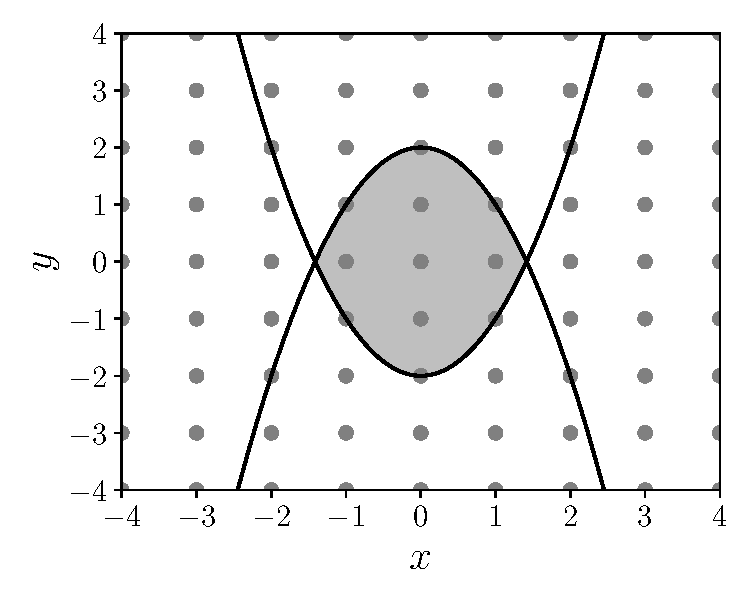
\includegraphics[totalheight=6cm]{chpt5/prob9.pdf}
  			  \caption{A visual representation of the set $C$ for Problems 9 and 10.}
    			   \label{fig:prob_9}
	\end{figure}
\begin{enumerate}

\item 

The joint PMF is:
\[
  P_{XY}(x, y) =
  \begin{cases}
                                   \frac{1}{11} & \text{for $(x, y) \in C$} \\
                                   0 & \text{otherwise} .
  \end{cases}
\]
By looking at Fig.~\ref{fig:prob_9} and adding vertically and horizontally, we can easily determine that the marginal PMFs are:
\[
  P_{X}(x) =
  \begin{cases}
                                   \frac{3}{11} & \text{for $x=-1$} \\
                                   \frac{5}{11} & \text{for $x=0$} \\
                                   \frac{3}{11} & \text{for $x=1$} 
  \end{cases}
\]
and
\[
  P_{Y}(y) =
  \begin{cases}
                                   \frac{1}{11} & \text{for $y=-2$} \\
                                   \frac{3}{11} & \text{for $y=-1$} \\
                                   \frac{3}{11} & \text{for $y=0$} \\
                                   \frac{3}{11} & \text{for $y=1$} \\
                                   \frac{1}{11} & \text{for $y=2$} .
  \end{cases}
\]

\item  Since there are 3 points at $Y=1$, and each point is equally as likely, the total probability mass at $Y=1$ is $3/11$, while the total probability mass at $(-1, 1), (0, 1), (1, 1)$ is 1/11 respectively.  Therefore:
\[
  P_{X|Y}(x|1) =
  \begin{cases}
                                   \frac{1}{3} & \text{for $x=-1$} \\
                                   \frac{1}{3} & \text{for $x=0$} \\
                                   \frac{1}{3} & \text{for $x=1$} .
  \end{cases}
\]

\item $X$ and $Y$ are not independent since, for example, at $X=-1$: $P(X=-1|Y=1) = 1/3 \neq P(X=-1) = 3/11$.

\item Using LOTUS, we have
\begin{equation*}
E[XY^2] = \sum_{(x, y) \in C} xy^2P_{XY}(x, y) = \frac{1}{11}\sum_{(x, y) \in C} xy^2 = \frac{1}{11} \left [1\cdot 1^2+1\cdot(-1)^2 -1\cdot1^2 -1\cdot(-1)^2\right]=0,
\end{equation*}
where only 4 points contribute to the sum (since the rest have zeros).

\end{enumerate}
\end{problem}

\begin{problem}{10} $ $

\begin{enumerate}

\item 

\begin{equation*}
E[X|Y=1] = \sum_{x \in R_{X|Y=1}} x P_{X|Y}(x|1) = (-1)\cdot \frac{1}{3}+(0)\cdot \frac{1}{3}+(1)\cdot \frac{1}{3} =0
\end{equation*}

\item

\begin{equation*}
Var[X|Y=1] = \sum_{x \in R_{X|Y=1}} x^2 P_{X|Y}(x|1) = (1)\cdot \frac{1}{3}+(0)\cdot \frac{1}{3}+(1)\cdot \frac{1}{3} = \frac{2}{3}
\end{equation*}

\item One can easily see that the PMF, $P_{X||Y| \le 1}(x)$ is exactly the same as the PMF for $P_{X|Y}(x|1)$, and therefore the expectation and variance will be the same, thus $E[X||Y| \le 1] =0$.

\item For the same reason as part c of this problem $E[X^2||Y| \le 1] =2/3$.

\end{enumerate}
\end{problem}


\begin{problem}{11} If there are $n$ cars in the shop, then $X = X_1+X_2+ \ldots+ X_n$, where $X_i$ is a $Bern(3/4)$ random variable (as specified in the problem), and where $X_1, X_2, \ldots, X_n$ are all independent (as specified in the problem).  Thus we have that $X|N=n \sim Bin(n, 3/4)$ and for the same reason, $Y|N=n \sim Bin(n, 1/4)$.

\begin{enumerate}

\item Noting that $R_X=R_Y = \{ 0, 1, 2, 3 \}$, we can use the law of total probability to find both of the marginal PMFs, which are:
\begin{align*}
P_X(x) &= \sum_{n=0}^3 P(X=x|N=n)P_N(n) \\
& =  \sum_{n=0}^3 \binom{n}{x} \left( \frac{3}{4} \right)^x \left(\frac{1}{4} \right)^{n-x}P_N(n),
\end{align*}
and 
\begin{align*}
P_Y(y) &= \sum_{n=0}^3 P(Y=y|N=n)P_N(n) \\
& =  \sum_{n=0}^3 \binom{n}{y} \left( \frac{1}{4} \right)^y \left(\frac{3}{4} \right)^{n-y}P_N(n).
\end{align*}
I compute both of these PMFs numerically to find:
\[
  P_{X}(x) \approx
  \begin{cases}
                                   0.180 & \text{for $x=0$} \\
                                   0.258 & \text{for $x=1$} \\
                                  0.352 & \text{for $x=2$} \\
                                  0.211& \text{for $x=3$} \\
                                  0& \text{otherwise},
   \end{cases}
\]
and
\[
  P_{Y}(y) \approx
  \begin{cases}
                                   0.570 & \text{for $y=0$} \\
                                   0.336 & \text{for $y=1$} \\
                                  0.086 & \text{for $y=2$} \\
                                  0.008& \text{for $y=3$} \\
                                  0& \text{otherwise},
   \end{cases}
\]
which, as a sanity, both add up to approximately 1.  We see that since a 4 door car is more likely than a 2 door car, the marginalized PMF for the 4 door cars skews towards high numbers, while the marginalized PMF for the 2 door cars skews towards lower numbers.

\item 

We can find the joint PMF for $X$ and $Y$ by conditioning on $N$ and using the law of total probability:
\begin{equation*}
P_{XY}(x, y) = \sum_{n=0}^3 P(X=x, Y=y|N=n)P_N(n),
\end{equation*}
where we can get rid of the sum because the probability is 0 if $x+y \ne n$:
\begin{align*}
P_{XY}(x, y) &=P(X=x, Y=y|N=x+y)P_N(x+y) \\
& = P(X=x|Y=y, N=x+y) P(Y=y|N=x+y)P_N(x+y) \\
& = P(Y=y|N=x+y)P_N(x+y) \\
& = \binom{x+y}{y}\left (\frac{1}{4} \right)^{y}\left (\frac{3}{4} \right)^{x} P_N(x+y),
\end{align*}
where in the second line I have used the chain rule of probability, in the third I have used the fact that given $Y=y$ and $N=x+y$, we are sure that $X=x$, and in the fourth line I have used the fact that $Y|N=x+y \sim Bin(x+y, 1/4)$.  I compute the joint PMF numerically and present the results in the following table:
\begin{center}
$P_{XY}(x, y) \approx $
\bgroup
\def\arraystretch{2.5}
 \begin{tabular}{ | c | c | c | c | c |}
    \hline
     & $Y=0$ & $Y=1$ & $Y=2$ & $Y=3$ \\  \hline
     $X=0$ &  0.125 &  0.031  &  0.016 &  0.008 \\ \hline
     $X=1$ & 0.094  &  0.094  &  0.070 &  0 \\ \hline
     $X=2$ &  0.141 &  0.211 &  0 &  0 \\ \hline
     $X=3$ & 0.211 &  0 &  0 &  0  \\
    \hline 
  \end{tabular}
  \egroup
\end{center}
As a check, I made sure that the above PMF sums to approximately 1.

\item $X$ and $Y$ are not independent since $P_{XY}(x, y) \ne  P_{X}(x) P_{Y}(y)$ $\forall x, y$.  For example $P_{XY}(0, 0) =0.125$, while $P_{X}(0)P_{Y}(0) \approx 0.180 \cdot 0.570 = 0.103$.

\end{enumerate}

\end{problem}


\begin{problem}{12} I first note that $R_X=R_Y=\{1, 2, 3, 4, 5 \}$ and $R_Z=\{-4, -3, \ldots, 3, 4 \}$.  I can find $P_Z(z)$ by conditioning on either $X$ or $Y$ and by using independence:
\begin{align*}
P_Z(z) &= P(Z = z) \\
& = P(Y=X-z) \\
& = \sum_{x=1}^5 P(Y=X-z|X=x)P_X(x) \\
& = \frac{1}{5}\sum_{x=1}^5 P(Y=x-z|X=x) \\
& = \frac{1}{5}\sum_{x=1}^5 P(Y=x-z) \\
& = \frac{1}{25}\sum_{x=1}^5 \mathbbm{1}\{x-z\in R_Y \},
\end{align*}  
where in going from the fourth to fifth line I used independence.  Thus we have:
\[
  P_{Z}(z) =
  \begin{cases}
                                   \frac{1}{25} & \text{for $z=-4$} \\
                                    \frac{2}{25} & \text{for $z=-3$} \\
                                   \frac{3}{25} & \text{for $z=-2$} \\
                                   \frac{4}{25} & \text{for $z=-1$} \\
                                   \frac{5}{25} & \text{for $z=0$} \\
                                    \frac{4}{25} & \text{for $z=1$} \\
                                     \frac{3}{25} & \text{for $z=2$} \\
                                      \frac{2}{25} & \text{for $z=3$} \\
                                       \frac{1}{25} & \text{for $z=4$}.
   \end{cases}
\]


\end{problem}



\begin{problem}{13} $ $
\begin{enumerate}

\item 

	\begin{equation*}  
  P_X(x) = \begin{cases}
                                   \frac{1}{6}+\frac{1}{6}+\frac{1}{8} & \text{for $x = 0$} \\
                                   \frac{1}{8}+\frac{1}{6}+\frac{1}{4} & \text{for $x = 1$} 
       \end{cases} \quad
= \begin{cases}
                                   \frac{11}{24}& \text{for $x = 0$} \\
                                   \frac{13}{24} & \text{for $x = 1$} 
       \end{cases}
\end{equation*}

	\begin{equation*}  
  P_Y(y) = \begin{cases}
                                   \frac{1}{6}+\frac{1}{8} & \text{for $y = 0$} \\
                                   \frac{1}{6}+\frac{1}{6} & \text{for $y = 1$} \\
                                   \frac{1}{8}+\frac{1}{4} & \text{for $y = 2$} 
       \end{cases} \quad
= \begin{cases}
                                   \frac{7}{24}& \text{for $y = 0$} \\
                                   \frac{1}{3} & \text{for $y = 1$} \\
                                   \frac{3}{8} & \text{for $y = 2$} 
       \end{cases}
\end{equation*}

\item

	\begin{equation*}  
  P_{X|Y}(x|0) = \begin{cases}
                                   \frac{\frac{1}{6}}{\frac{1}{6}+\frac{1}{8}}& \text{for $x = 0$} \\
                                   \frac{\frac{1}{8}}{\frac{1}{6}+\frac{1}{8}}& \text{for $x = 1$} 
       \end{cases} \quad
= \begin{cases}
                                   \frac{4}{7}& \text{for $x = 0$} \\
                                   \frac{3}{7} & \text{for $x = 1$} 
       \end{cases}
\end{equation*}

	\begin{equation*}  
  P_{X|Y}(x|1) = \begin{cases}
                                   \frac{\frac{1}{6}}{\frac{1}{6}+\frac{1}{6}}& \text{for $x = 0$} \\
                                   \frac{\frac{1}{6}}{\frac{1}{6}+\frac{1}{6}}& \text{for $x = 1$} 
       \end{cases} \quad
= \begin{cases}
                                   \frac{1}{2}& \text{for $x = 0$} \\
                                   \frac{1}{2} & \text{for $x = 1$} 
       \end{cases}
\end{equation*}

	\begin{equation*}  
  P_{X|Y}(x|2) = \begin{cases}
                                   \frac{\frac{1}{8}}{\frac{1}{8}+\frac{1}{4}}& \text{for $x = 0$} \\
                                   \frac{\frac{1}{4}}{\frac{1}{8}+\frac{1}{4}}& \text{for $x = 1$} 
       \end{cases} \quad
= \begin{cases}
                                   \frac{1}{3}& \text{for $x = 0$} \\
                                   \frac{2}{3} & \text{for $x = 1$} 
       \end{cases}
\end{equation*}

\item We know that

\[
  Z =
  \begin{cases}
                                   E[X|Y=0]& \text{with probability $P_Y(0)$} \\
                                   E[X|Y=1]& \text{with probability $P_Y(1)$} \\
                                  E[X|Y=2]& \text{with probability $P_Y(2)$},
   \end{cases}
\]
or in other words:
 \[
  P_{Z}(z) =
  \begin{cases}
                                   P_Y(0) & \text{for $z=E[X|Y=0]$} \\
                                    P_Y(1) & \text{for $z=E[X|Y=1]$} \\
                                   P_Y(2) & \text{for $z=E[X|Y=2]$}.
   \end{cases}
\]
We already know the marginal PMF of $Y$, and thus what is left to calculate is $E[X|Y=y]$ for all $y \in R_Y$:
\begin{align*}
E[X|Y=0] &= \sum_{x \in R_X} x P_{X|Y}(x|0) \\
& = 0 \left(\frac{4}{7} \right)+1 \left(\frac{3}{7} \right) \\
& = \frac{3}{7},
\end{align*}
\begin{align*}
E[X|Y=1] &= \sum_{x \in R_X} x P_{X|Y}(x|1) \\
& = 0 \left(\frac{1}{2} \right)+1 \left(\frac{1}{2} \right) \\
& = \frac{1}{2},
\end{align*}
\begin{align*}
E[X|Y=2] &= \sum_{x \in R_X} x P_{X|Y}(x|2) \\
& = 0 \left(\frac{1}{3} \right)+1 \left(\frac{2}{3} \right) \\
& = \frac{2}{3}.
\end{align*}
Finally, we have that:
 \[
  P_{Z}(z) =
  \begin{cases}
                                   \frac{7}{24}& \text{for $z=\frac{3}{7}$} \\
                                    \frac{1}{3} & \text{for $z=\frac{1}{2}$} \\
                                   \frac{3}{8} & \text{for $z=\frac{2}{3}$}.
   \end{cases}
\]


\item For this problem we are checking that the law of iterated expectations holds.  That is, we need to check explicitly that $E[X] = E[E[X|Y]]$, where the outer expectation on the RHS is over $Y$.  Computing the LHS I have:
\begin{equation*}
E[X] = \sum_{x \in R_X} x P_X(x) = 0\left (\frac{11}{24} \right)+1\left (\frac{13}{24} \right) = \frac{13}{24}.
\end{equation*}
Computing the RHS I have:
\begin{align*}
E[Z] &= E_Y[E[X|Y]] \\
& = \sum_{y \in R_Y} E[X|Y=y] P_Y(y) \\
&=\left ( \frac{3}{7} \right ) \left (\frac{7}{24} \right)+\left ( \frac{1}{2} \right ) \left (\frac{1}{3} \right)+\left ( \frac{2}{3} \right ) \left (\frac{3}{8} \right) \\
& = \frac{13}{24}.
\end{align*}
The LHS and RHS agree, and thus the law of iterated expectations holds.

\item 

\begin{align*}
E[Z^2] &= \sum_{z \in R_Z} z^2 P_Z(z) \\
& = \left ( \frac{3}{7} \right )^2 \left (\frac{7}{24} \right)+\left ( \frac{1}{2} \right )^2 \left (\frac{1}{3} \right)+\left ( \frac{2}{3} \right )^2 \left (\frac{3}{8} \right) \\
& =\frac{17}{56}
\end{align*}
$\implies$
\begin{equation*}
Var[Z] = E[Z^2] - E[Z]^2 =  \frac{17}{56} - \left( \frac{13}{24}\right)^2 =\frac{41}{4032}
\end{equation*}

\end{enumerate}
\end{problem}


\begin{problem}{14} $ $
\begin{enumerate}


\item As with the previous problem, we know that

\[
  V =
  \begin{cases}
                                   Var[X|Y=0]& \text{with probability $P_Y(0)$} \\
                                   Var[X|Y=1]& \text{with probability $P_Y(1)$} \\
                                  Var[X|Y=2]& \text{with probability $P_Y(2)$},
   \end{cases}
\]
or in other words:
 \[
  P_{V}(v) =
  \begin{cases}
                                   P_Y(0) & \text{for $v=Var[X|Y=0]$} \\
                                    P_Y(1) & \text{for $v=Var[X|Y=1]$} \\
                                   P_Y(2) & \text{for $v=Var[X|Y=2]$}.
   \end{cases}
\]
Thus, we must compute $Var[X|Y=y] = E[X^2|Y=y]+E[X|Y=y]^2$ for all $y \in R_Y$.  $E[X|Y=y]$ was already computed in the previous problem, and, since to compute $E[X^2|Y=y]$, both terms in the summation are the same as the two terms in the summation to compute $E[X|Y=y]$ (since $0^2=0$ and $1^2=1$), we have that $E[X^2|Y=y]=E[X|Y=y]$ (this can be seen more clearly if one explicitly writes out the summation for $E[X^2|Y=y]$).  Thus we have that:
\begin{equation*}
Var[X|Y=0] =  E[X^2|Y=0]-E[X|Y=0]^2 = \frac{3}{7} -\left ( \frac{3}{7} \right)^2 = \frac{12}{49},
\end{equation*}
\begin{equation*}
Var[X|Y=1] =  E[X^2|Y=1]-E[X|Y=1]^2 = \frac{1}{2} -\left ( \frac{1}{2} \right)^2 = \frac{1}{4},
\end{equation*}
and
\begin{equation*}
Var[X|Y=2] =  E[X^2|Y=2]-E[X|Y=2]^2 = \frac{2}{3} -\left ( \frac{2}{3} \right)^2 = \frac{2}{9}.
\end{equation*}
The PMF for $V$ is thus
 \[
  P_{V}(v) =
  \begin{cases}
                                   \frac{7}{24} & \text{for $v=\frac{12}{49}$} \\
                                    \frac{1}{3} & \text{for $v=\frac{1}{4}$} \\
                                   \frac{3}{8} & \text{for $v=\frac{2}{9}$}.
   \end{cases}
\]

\item
\begin{equation*}
E[V] = \sum_{v \in R_V}v P_V(v) = \frac{12}{49}\cdot \frac{7}{24}+ \frac{1}{4}\cdot \frac{1}{3}+ \frac{2}{9}\cdot \frac{3}{8} =\frac{5}{21}
\end{equation*}

\item In this problem we are checking that the law of total variance, $Var[X] = E_Y[Var[X|Y]]+Var_Y[E[X|Y]]$, holds (where the subscript $Y$ on the expectation and variance denotes with respect to the random variable $Y$.)  Computing the LHS:
\begin{align*}
Var[X] &= E[X^2]-E[X]^2\\
& = \sum_{x \in R_X}x^2 P_X(x)- \left[\sum_{x \in R_X}x P_X(x)\right]^2 \\
& = 0^2\cdot \frac{11}{24}+1^2\cdot \frac{13}{24}-\left[ 0\cdot \frac{11}{24}+1\cdot \frac{13}{24} \right]^2\\
&=\frac{143}{576}.
\end{align*}
Computing the RHS:
\begin{align*}
E_Y[Var[X|Y]]+Var_Y[E[X|Y]] & = E[V]+Var[Z] \\
& = \frac{5}{21}+\frac{41}{4032} \\
& = \frac{143}{576},
\end{align*}
which is in agreement with the LHS of the equation.  Note that $E[V]$ and $Var[Z]$ were computed in this problem and the previous problem.

\end{enumerate}
\end{problem}



\begin{problem}{15} The law of total expectation gives:
\begin{align*}
E[Y] &= \sum_{n=0}^\infty E[Y|N=n]P_N(n) \\
& = \sum_{n=0}^\infty E\left [\sum_{i=1}^N X_i|N=n \right ]P_N(n) \\
& = \sum_{n=0}^\infty E\left [\sum_{i=1}^n X_i \right ]P_N(n) \\
& = \sum_{n=0}^\infty  \sum_{i=1}^n E[X_i] P_N(n) \\
& = \sum_{n=0}^\infty  \sum_{i=1}^n E[X_i] \frac{e^{-\beta} \beta^n}{n!} \\
& = \sum_{n=0}^\infty  \sum_{i=1}^n \frac{1}{\lambda} \frac{e^{-\beta} \beta^n}{n!} \\
& =\frac{e^{-\beta}}{\lambda} \sum_{n=0}^\infty \frac{n \beta^n}{n!},
\end{align*}
where in going from the second to the third line I have used the fact that $X_i$ and $N$ are independent (for all $i$), in going from the third to the fourth line I have used the linearity of expectation, and in going from the fifth to sixth line I have used the fact that for an $Exp(\lambda)$ distribution, $E[X] = 1/\lambda$ .  This summation can be computed by considering the Taylor expansion of the exponential, $\exp(x) = \sum_{n=0}^\infty (x^n)/n!$.  Taking the derivative of both sides of this formula with respect to $x$, we find that the desired sum is:
\begin{equation*}
 \sum_{n=0}^\infty \frac{n x^n}{n!} = xe^x,
\end{equation*}
and hence
\begin{equation*}
E[Y] = \frac{\beta}{\lambda}.
\end{equation*} 
The calculation for $Var[Y]$ is similar.  For this calculation, we will need $\sum_{n=0}^\infty (n^2 x^n)/n!$, which can be found with the same differentiation strategy.  I differentiate the equation for the previous summation with respect to $x$ once more and solve for the desired summation to find
\begin{equation*}
 \sum_{n=0}^\infty \frac{n^2 x^n}{n!} = xe^x+x^2e^x,
\end{equation*}
where I have used the chain rule in differentiating.

To find $Var[Y]$ I now solve for $E[Y^2]$, which is only moderating more complicated than solving for $E[Y]$.  The law of total expectation gives:
\begin{align*}
E[Y^2] &= \sum_{n=0}^\infty E[Y^2|N=n]P_N(n) \\
& = \sum_{n=0}^\infty E\left [\left ( \sum_{i=1}^N X_i \right )^2|N=n \right ]P_N(n) \\
& = \sum_{n=0}^\infty E\left [\left ( \sum_{i=1}^n X_i \right )^2 \right ]P_N(n) \\
& = \sum_{n=0}^\infty E\left [\sum_{i=1}^n X_i^2+ \sum_{j, k: j \neq k} X_j X_k\right ]P_N(n) \\
& = \sum_{n=0}^\infty \left \{\sum_{i=1}^n E[X_i^2]+ \sum_{j, k: j \neq k}  E[X_j X_k] \right \}P_N(n) \\
& = \sum_{n=0}^\infty \left \{\sum_{i=1}^n E[X_i^2]+ \sum_{j, k: j \neq k}  E[X_j] E[X_k] \right \}P_N(n) \\
& = \sum_{n=0}^\infty \left \{\sum_{i=1}^n \frac{2}{\lambda^2}+\sum_{j, k: j \neq k} \frac{1}{\lambda^2} \right \}P_N(n) \\
& = \sum_{n=0}^\infty \left [ \frac{2n}{\lambda^2}+ \frac{n^2-n}{\lambda^2} \right ]\frac{e^{-\beta} \beta^n}{n!} \\
& = \frac{e^{-\beta}}{\lambda^2}\sum_{n=0}^\infty \frac{n \beta^n}{n!}+ \frac{e^{-\beta}}{\lambda^2}\sum_{n=0}^\infty \frac{n^2 \beta^n}{n!},
\end{align*}
where in going from the second to third line I have used the fact that $X_i$ and $N$ are independent (for all $i$), in going from the third to fourth line I have broken the square of the summation into the summation of the squares plus the summation of the cross-terms.  The notation $\sum_{j, k: j \neq k}$ denotes a sum over all possible tuples of $(j,k)$, where $j, k =1, 2, \ldots, n$, except the tuples where $j=k$. In going from the fourth to fifth line I have used the linearity of expectation, in going from the fifth to sixth line I have used the independence of all $X_i$s, and in going from the sixth to seventh line I have used the fact that for an $Exp(\lambda)$ distribution, $E[X^2] = 2/\lambda^2$ (as calculated in the book).  The first summation summation has already been solved for, and to solve the second summation, I use the formula for $\sum_{n=0}^\infty \frac{n^2 x^n}{n!} $ as derived above.  Thus I have that
\begin{align*}
E[Y^2] &= \frac{1}{\lambda} \cdot \frac{\beta}{\lambda}+ \frac{e^{-\beta}}{\lambda^2} \left (\beta e^{\beta}+\beta^2 e^{\beta} \right) \\
& = \frac{\beta^2 +2 \beta}{\lambda^2}.
\end{align*}
Finally we have that:
\begin{align*}
Var[Y] &=  E[Y^2]  -E[Y]^2 \\
&=  \frac{\beta^2 +2 \beta}{\lambda^2} -\frac{\beta^2}{\lambda^2} \\
& = \frac{2 \beta}{\lambda^2}.
\end{align*}

\end{problem}


\begin{problem}{16} $ $
\begin{enumerate}

\item 
\begin{align*}
1 &= \int_0^1 \int_0^\infty f_{XY}(x, y)dx dy \\
& = \int_0^1 \int_0^\infty \frac{1}{2}e^{-x} dx dy+c\int_0^1 \int_0^\infty \frac{y}{(1+x)^2}dx dy \\
& = \int_0^1 \int_0^\infty \frac{1}{2}e^{-x} dx dy+c\int_0^1 \int_1^\infty \frac{y}{u^2}du dy \\
& = \frac{1}{2}+\frac{c}{2}
\end{align*}
$\implies$
\begin{equation*}
c = 1
\end{equation*}


\item 
\begin{align*}
P\left(0 \le X \le 1, 0 \le Y \le \frac{1}{2} \right) &= \int_0^{1/2} \int_0^{1} f_{XY}(x, y)dx dy \\
&= \int_0^{1/2} \int_0^{1} \left [ \frac{1}{2}e^{-x} + \frac{y}{(1+x)^2} \right ]dx dy \\
& = \frac{1}{4}(1-e^{-1})+\frac{1}{16}\\
& \approx 0.22
\end{align*}

\item 
\begin{align*}
P(0 \le X \le 1) &= \int_0^{1} \int_0^{1} f_{XY}(x, y)dx dy \\
&= \int_0^{1} \int_0^{1} \left [ \frac{1}{2}e^{-x} + \frac{y}{(1+x)^2} \right ]dx dy \\
& = \frac{1}{2}(1-e^{-1})+\frac{1}{4}\\
& \approx 0.57
\end{align*}



\end{enumerate}
\end{problem}


\begin{problem}{17} $ $
\begin{enumerate}

\item 

\begin{align*}
f_X(x) &= \int_{R_Y} f_{XY}(x, y)dy \\
&= \int_{0}^\infty e^{-xy}dy \\
&= -\left( \frac{e^{-xy}}{x}\right)_0^\infty \\
& = \frac{1}{x}
\end{align*}
$\implies$
\[
  f_X(x) =
  \begin{cases}
                                   \frac{1}{x}& \text{for $1 \le x< e$} \\
                                   0& \text{otherwise}
   \end{cases}
\]

\begin{align*}
f_Y(y) &= \int_{R_X} f_{XY}(x, y)dx \\
&= \int_{1}^e e^{-xy}dx \\
&= -\left( \frac{e^{-xy}}{y}\right)_1^e \\
& = \frac{1}{y} \left(\frac{1}{e^y}-\frac{1}{e^{ey}} \right)
\end{align*}
$\implies$
\[
  f_Y(y) =
  \begin{cases}
                                    \frac{1}{y} \left(\frac{1}{e^y}-\frac{1}{e^{ey}} \right)& \text{for $y>0$} \\
                                   0& \text{otherwise}
   \end{cases}
\]

\item 

\begin{equation*}
P(0 \le Y \le 1, 1 \le X\le \sqrt{e}) = \int_0^1\int_1^{\sqrt{e}} e^{-xy} dx dy
\end{equation*}



\end{enumerate}
\end{problem}

\begin{problem}{18} $ $
\begin{enumerate}


\item
\begin{align*}
f_X(x) &= \int_{R_Y} f_{XY}(x, y)dy \\
&= \int_{0}^2 \left(\frac{1}{4}x^2+\frac{1}{6}y \right )dy \\
& = \frac{1}{2}x^2+\frac{1}{3}
\end{align*}
$\implies$
\[
  f_X(x) =
  \begin{cases}
                                    \frac{1}{2}x^2+\frac{1}{3}& \text{for $-1 \le x\le 1$} \\
                                   0& \text{otherwise}
   \end{cases}
\]


\begin{align*}
f_Y(y) &= \int_{R_X} f_{XY}(x, y)dx \\
&= \int_{-1}^1 \left(\frac{1}{4}x^2+\frac{1}{6}y \right )dx \\
& = \frac{1}{3}y+\frac{1}{6}
\end{align*}
$\implies$
\[
  f_Y(y) =
  \begin{cases}
                                    \frac{1}{3}y+\frac{1}{6}& \text{for $0 \le y\le 2$} \\
                                   0& \text{otherwise}
   \end{cases}
\]

\item
\begin{align*}
P(X>0, Y<1) &= \int_{0}^1 \int_0^1\left( \frac{1}{4}x^2+\frac{1}{6}y \right)dxdy \\
&= \frac{1}{6}
\end{align*}

\item Using inclusion-exclusion:
\begin{align*}
P(X>0 \cup Y<1) &= P(X>0)+P(Y<1)-P(X>0, Y<1)\\
& = \int_{0}^1 \int_0^2\left( \frac{1}{4}x^2+\frac{1}{6}y \right)dydx +\int_{-1}^1 \int_0^1\left( \frac{1}{4}x^2+\frac{1}{6}y \right)dydx -\frac{1}{6} \\
&\frac{1}{2}+\frac{1}{3} -\frac{1}{6} \\
&= \frac{2}{3}.
\end{align*}

\item
\begin{align*}
P(X>0|Y<1) &= \frac{P(X>0, Y<1)}{P(Y<1)}\\
& = \frac{\frac{1}{6}}{\frac{1}{3}} \\
&= \frac{1}{2}.
\end{align*}

\item
We must be slightly care in choosing the bounds of integration for this problem.  The upper bound of the $y$ integral is the upper bound of $R_Y$, and the lower bound of the $y$ integral is $\max \{0, -x\}$, and not simply $-x$.  This is because for $x>0$, $-x<0$, but the lower bound of the range of $Y$ is 0.  An illustration of the domain of the double integral is shown in Fig.~\ref{fig:prob_18}.  The probability we seek is thus:

\begin{align*}
P(X+Y>0) &= P(Y>-X)\\
& = \int_{-1}^1 \int_{\max \{0, -x\} }^2\left( \frac{1}{4}x^2+\frac{1}{6}y \right)dydx \\
&= \int_{-1}^1 \left [\frac{1}{4}x^2 y +\frac{1}{12}y^2 \right]_{\max \{ 0, -x \} }^2 dx \\
&= \frac{1}{4}\int_{-1}^1 x^2 \left(2-\max \{0, -x\} \right) dx+ \frac{1}{12}\int_{-1}^1 \left(4-\max \{0, -x\}^2 \right) dx \\
&= \frac{1}{4}\int_{-1}^0 x^2 \left(2+x \right) dx+ \frac{1}{4}\int_{0}^1 2 x^2 dx+ \frac{1}{12}\int_{-1}^0 \left(4-x^2 \right) dx+\frac{1}{12}\int_{0}^1 4 dx \\
& = \frac{131}{144}.
\end{align*}

	\begin{figure}[t]
	\centering
      		 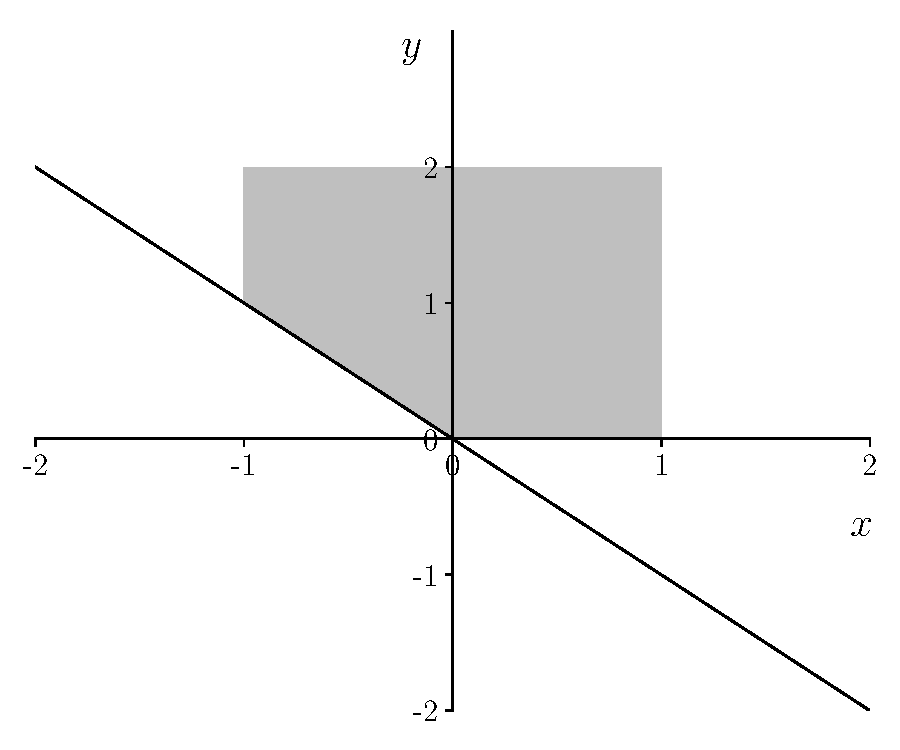
\includegraphics[totalheight=6cm]{chpt5/prob18.pdf}
  			  \caption{The region of integration for Problem 18 (e) (shaded region).}
    			   \label{fig:prob_18}
	\end{figure}

\end{enumerate}
\end{problem}


\begin{problem}{19} $ $
\begin{enumerate}
\item 
\begin{align*}
f_{XY}(x, y) &= \frac{\partial F_{XY}}{\partial x \partial y} \\
& = e^{-x}2e^{-2y}
\end{align*}
$\implies$
\[
  f_{XY}(x, y) =
  \begin{cases}
                                   e^{-x}2e^{-2y}& \text{for $x, y>0$} \\
                                   0& \text{otherwise}
   \end{cases}
\]


\item 
\begin{align*}
P\left(Y>\frac{1}{2}X\right) &= \int_0^\infty \int_0^{x/2}e^{-x}2e^{-2y}dydx \\
& = \int_0^\infty\left(e^{-x}-e^{-2x} \right)dx \\
&=\frac{1}{2}
\end{align*}

\item
$X$ and $Y$ are independent because the joint PDF can be factored into the product of 2 marginal PDFs.  Specifically, the joint PDF can be factored into $f_X(x)f_Y(y)$ where $X\sim Exp(1)$ and where where $Y\sim Exp(2)$.


\end{enumerate}
\end{problem}

\begin{problem}{20} $ $
\begin{enumerate}
\item
To calculate the PDF, we simply need to condition on $X>0$, and since a $\mathcal N(0, 1)$ distribution is symmetric about zero, we know that $P(X>0) =1/2$:
\begin{align*}  
f_{X|X>0}(x) &=\frac{f_X(x)}{P(X>0)} \\
& = \begin{cases}
                                   \frac{2}{\sqrt{2 \pi}} e^{-\frac{x^2}{2}} & \text{for $x >0$} \\
                                   0 & \text{otherwise}.
       \end{cases} \quad
       \end{align*}
To find the conditional CDF, we need only to integrate the Gaussian:
\begin{align*}
F_{X|X>0}(x) &= 2 \int_0^x \frac{1}{\sqrt{2 \pi}}e^{-\frac{{x^\prime}^2}{2}}dx^\prime \\
& =2\left[ \Phi(x) -\frac{1}{2} \right],
\end{align*}
so that
\[
 F_{X|X>0}(x) =
  \begin{cases}
                                   2\Phi(x) -1 & \text{for $x>0$} \\
                                   0& \text{otherwise}.
   \end{cases}
\]

\item
\begin{align*}
E[X|X>0] &= \int_0^\infty x f_{X|X>0}(x)dx \\
& = \frac{2}{\sqrt{2 \pi}} \int_0^\infty x e^{-\frac{x^2}{2}}dx \\
& = \frac{1}{\sqrt{2 \pi}} \int_0^\infty e^{-\frac{u}{2}}du \\
& = \frac{2}{\sqrt{2 \pi}}
\end{align*}


\item We can compute $E[X^2|X>0]$ by noting that if $Y \sim \mathcal N(0, 1)$, then:
\begin{align*}
1 &= E[Y^2] \\
& =\frac{2}{\sqrt{2 \pi} } \int_0^\infty y^2 e^{-\frac{y^2}{2}}dy,
\end{align*}
where I have used the fact that $y^2$ times $\exp{(-y^2/2)}$ is an even function, so I need only integrate from 0 to infinity and multiply by 2.  Thus we have that 
\begin{align*}
E[X^2|X>0] &= \int_0^\infty x^2 f_{X|X>0}(x)dx \\
& = \frac{2}{\sqrt{2 \pi}} \int_0^\infty x^2 e^{-\frac{x^2}{2}}dx \\
& = 1.
\end{align*}
Finally, we have that:
\begin{align*}
Var[X|X>0] &= E[X^2|X>0] -(E[X|X>0] )^2 \\
&=1- \left(\frac{2}{\sqrt{2 \pi}}\right)^2 \\
& =\frac{\pi-2}{\pi}.
\end{align*}

\end{enumerate}

\end{problem}

\begin{problem}{21} $ $
\begin{enumerate}
\item I first find the marginal PDF of $Y$:
\begin{align*}
f_Y(y) &= \int_{-1}^{1} \left(x^2+\frac{1}{3}y\right)dx \\
& =\frac{2}{3}(1+y),
\end{align*}
so that we have
\begin{align*}
f_{X|Y}(x|y) &= \frac{f_{XY}(x,y)}{f_Y(y)} \\
& =\frac{x^2+\frac{1}{3}y}{\frac{2}{3} (1+y)},
\end{align*}
and therefore:
\[
 f_{X|Y}(x|y) =
  \begin{cases}
                                   \frac{3x^2+y}{ 2(1+y)} & \text{for $-1 \le x \le 1$} \\
                                   0& \text{otherwise}.
   \end{cases}
\]



\item 
\begin{align*}
P(X>0|Y=y) &= \int_0^1 f_{X|Y}(x|y)dx \\
&\frac{1}{2(1+y)} \int_0^1 \left(3x^2+y \right) dx \\
& =\frac{1}{2}.
\end{align*}
Notice that the probability, $P(X>0|Y=y)$, does not depend on $y$.

\item We have already found the marginal PDF of $Y$, and now I find the marginal PDF of $X$:
\begin{align*}
f_X(x) &= \int_{0}^{1} \left(x^2+\frac{1}{3}y\right)dy \\
& =x^2 +\frac{1}{6}.
\end{align*}
We thus see that $f_X(x)f_Y(y) = 2x^2/3+y/9+2 y x^2/3+1/9 \ne f_{XY}(x, y)$, and so $X$ and $Y$ are not independent.

\end{enumerate}
\end{problem}


\begin{problem}{22} I start by first finding the marginal PDF of $X$:
\begin{align*}
f_X(x) &= \int_0^1 \left(\frac{1}{2}x^2+\frac{2}{3}y\right)dy \\
& =\frac{1}{2}x^2 +\frac{1}{3},
\end{align*}
which is valid for $-1 \le x \le 1$, otherwise $f_X(x) =0.$

I now find the PDF of $Y$ conditioned on $X=0$:
\begin{align*}
f_{Y|X}(y|0) &= \frac{f_{XY}(0, y)}{f_X(0)} \\
& = \frac{\frac{2}{3}y}{\frac{1}{3}} \\
& = 2y
\end{align*}
valid for $0\le y \le 1$.  I may now calculate $E[Y|X=0],$
\begin{align*}
E[Y|X=0] &= \int_{R_{Y|X=0}} y f_{Y|X}(y|0) dy \\
& = \int_{0}^1 2y^2 dy  \\
& = \frac{2}{3},
\end{align*}
and $E[Y^2|X=0],$
\begin{align*}
E[Y^2|X=0] &= \int_{R_{Y|X=0}} y^2 f_{Y|X}(y|0) dy \\
& = \int_{0}^1 2 y^3 dy  \\
& = \frac{1}{2}.
\end{align*}
Therefore, the variance is: $Var[Y|X=0] = E[Y^2|X=0] - (E[Y|X=0])^2 = 1/2 - (2/3)^2 = 1/18.$

\end{problem}







\begin{problem}{23} $ $
\begin{enumerate}

\item The set $E$ is a diamond shaped region in $\mathbb R^2$, upper-bounded by $1-|x|$ and lower-bounded by $|x|-1$, as shown in Fig.~\ref{fig:prob_23}.  The area of the region is thus 4 times the area of a triangle with a base length of 1 and height length of 1: $4\cdot(1/2)\cdot(1)\cdot(1)=2$.  Since the total probability must integrate to unity, we thus have $c=1/2$.

	\begin{figure}[t]
	\centering
      		 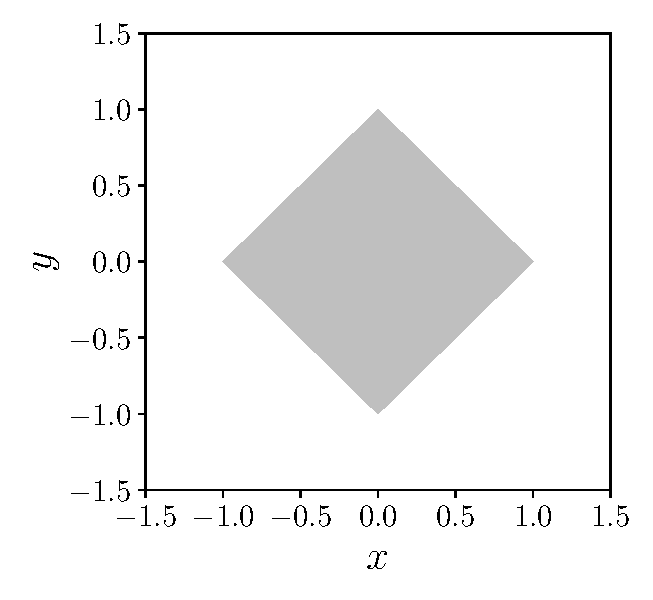
\includegraphics[totalheight=7cm]{chpt5/prob23.pdf}
  			  \caption{A visual representation of the set $E$ for Problem 23.}
    			   \label{fig:prob_23}
	\end{figure}

\item
The marginal PDF of $X$ is given by 
\begin{align*}
f_X(x) &= 2\int_0^{1-|x|} \frac{1}{2} dy \\
& =1-|x|,
\end{align*}
so, that
\[
 f_X(x) =
  \begin{cases}
                                   1-|x| & \text{for $-1 \le x \le 1$} \\
                                   0& \text{otherwise}.
   \end{cases}
\]
By symmetry, we also know that 
\[
 f_Y(y) =
  \begin{cases}
                                   1-|y| & \text{for $-1 \le y \le 1$} \\
                                   0& \text{otherwise}.
   \end{cases}
\]

\item
The conditional PDF is given by
\begin{align*}  
  f_{X|Y}(x|y)&= \frac{f_{XY}(x, y)}{f_Y(y)}\\
& = \begin{cases}
                                   \frac{1}{2(1-|y|)}& \text{for $x, y \in E$} \\
                                   0 & \text{otherwise}.
       \end{cases} \quad
       \end{align*}

\item $X$ and $Y$ are not independent, as it is clear that $f_{X|Y}(x|y) \ne f_X(x)  $.
\end{enumerate}
\end{problem}

\begin{problem}{24}  The marginal PDFs for $X$ and $Y$ are given by 
\[
 f_X(x) =
  \begin{cases}
                                   \frac{1}{2} & \text{for $0 \le x \le 2$} \\
                                   0& \text{otherwise},
   \end{cases}
\]
and
\[
 f_Y(y) =
  \begin{cases}
                                   \frac{1}{2} & \text{for $0 \le y \le 2$} \\
                                   0& \text{otherwise}.
   \end{cases}
\]
I solve for the desired probability by conditioning on $Y$ and using the fact that $X$ and $Y$ are independent:
\begin{align*}
P(XY<1) &= \int_0^2P(XY<1|Y=y)f_Y(y)dy \\
&= \int_0^2P(Xy<1)f_Y(y)dy \\
&= \int_0^2P\left(X<\frac{1}{y}\right)f_Y(y)dy \\
&= \int_0^2 \int_0^{\min \{ 2, 1/y \} }f_X(x) f_Y(y)dxdy \\
&= \frac{1}{4}\int_0^2 \min \left \{ 2, \frac{1}{y} \right \}dy \\
&= \frac{1}{4}\left(\int_0^{1/2}2dy+\int_{1/2}^{2}\frac{1}{y}dy \right)\\
& = \frac{1}{4}+\frac{\ln 2}{2} \\
& \approx 0.60.
\end{align*}

\end{problem}

\begin{problem}{25} The easiest way to solve this problem will be to use the law of iterated expectations and the law of total variance.  The following information will be useful: for $X\sim Exp(1)$, $E[X]=1$, $Var[X]=1$ and $E[X^2]=2$, and for $Y|X \sim Unif(0, X)$, $E[Y|X]=X/2$ and $Var[Y|X] = X^2/12$.
\begin{enumerate}

\item I use the law of iterated expectations, where the subscript on the first expectation denotes an expectation over $X$:
\begin{align*}
E[Y] &= E_X[E[Y|X]] \\
& = E_X\left[\frac{X}{2} \right]\\
& = \frac{1}{2}.
\end{align*}

\item I use the law of total variance, where the subscripts denote expectation and variance over $X$:
\begin{align*}
Var[Y] &= E_X[Var[Y|X]] +Var_X[E[Y|X]]\\
& = E_X\left[\frac{X^2}{12} \right]+Var_X\left[\frac{X}{2} \right]\\\
& = \frac{5}{12}.
\end{align*}

\end{enumerate}
\end{problem}

\begin{problem}{26} For $X \sim Unif(0,1)$ we have: $E[X]=1/2$ and $E[X^2]=1/3$. 
\begin{enumerate}

\item Since $X$ and $Y$ are independent, the expectation of the product is the product of the expectations:
\begin{align*}
E[XY] &= E[X]E[Y] \\
& = \frac{1}{4}.
\end{align*}

\item Since $X$ and $Y$ are independent $E[g(X)h(Y)]=E[g(X)]E[h(Y)]$:
\begin{align*}
E[e^{X+Y}] &= E\left [e^Xe^Y \right] \\
&= E\left [e^X \right ]E\left [e^Y \right]. 
\end{align*}
I can compute $E[e^X]$ using LOTUS:
\begin{align*}
E\left[e^{X}\right] &= \int_0^1 e^x dx \\
& = e-1,
\end{align*}
and plugging into the previous equation I find that
\begin{equation*}
E\left[e^{X+Y}\right] = (e-1)^2.
\end{equation*}

\item 
\begin{align*}
E[X^2+Y^2+XY] &= E[X^2]+E[Y^2]+E[XY] \\
& = \frac{1}{3}+\frac{1}{3}+\frac{1}{4} \\
& = \frac{11}{12}
\end{align*}

\item We can compute this expectation with a 2D LOTUS over the joint distribution of $X$ and $Y$.  Since $X$ and $Y$ are independent, $f_{XY}(x,y) = f_X(x)f_Y(y) = 1$ for $x, y \in [0, 1]$:
\begin{align*}
E[Ye^{XY}] &= \int_0^1 \int_0^1 y e^{xy} dxdy \\
&= \int_0^1 \left (1-e^y \right) dy \\
&= e-2.
\end{align*}

\end{enumerate}
\end{problem}

\begin{problem}{27} I first note that $R_X=R_Y=[0, 1]$ and that $R_Z=[0, \infty)$.  I solve for the CDF of $Z$ by conditioning on $X$ and using the fact that $X$ and $Y$ are independent:
\begin{align*}
F_Z(z) &= P(Z \le z) \\
& = P\left(\frac{X}{Y} \le z\right) \\
& = P\left(Y \ge \frac{X}{z}\right) \\
& = \int_{-\infty}^\infty P \left(Y \ge \frac{x}{z} |X=x\right)f_X(x)dx \\
& = \int_{0}^1 P\left(Y \ge \frac{x}{z}|X=x\right)dx \\
& = \int_{0}^1 P\left(Y \ge \frac{x}{z}\right)dx,
\end{align*}
where in the last line I have used the fact that $X$ and $Y$ are independent.  To solve for $P(Y \ge X/z)$ by integrating $F_Y(y)$ over $y$, some care must be taken in the limits of integration.  Since $x \in [0, 1]$ and $z \in [0, \infty)$, this implies that $x/z \in [0, \infty)$.  However, we know that $f_Y(y) = 0$ for $y>1$ and thus the lower bound of integration is not simply $x/z$, but is $\min \{1, x/z \}$.  This can be seen pictorially in Fig.~\ref{fig:prob_27} a) (from a point of view of integrating over the joint PDF to solve the problem, rather than the conditional PDF), which is the $x-y$ plane, where the grey region corresponds to the region of non-zero joint probability density.  For any given $z$, $P(Y \ge X/z)$ represents the total probability mass above the the line defined by $x/z$.  For example, I have, I have drawn 3 different lines in \ref{fig:prob_27} a) corresponding to $z=1/2$ (highest line), $z=1$ (middle line) and $z=2$ (lowest line).  For each of these $z$ values, $P(Y \ge X/z)$ is the fraction of the grey box above that line.  We see that when $z$ increases from $0$ to $1$ (corresponding to the vertical  line along the $y$-axis and the line $y=x$), the total probability mass above the line increases smoothly.  However, due to the edge of the box, there is a kink in the total probability mass above the line when transitioning from $z<1$ to $z>1$, which is the same reason we will get a kink in the function $F_Z(z)$ due to $\min \{1, x/z \}$.  

	\begin{figure}[t]
	\centering
      		 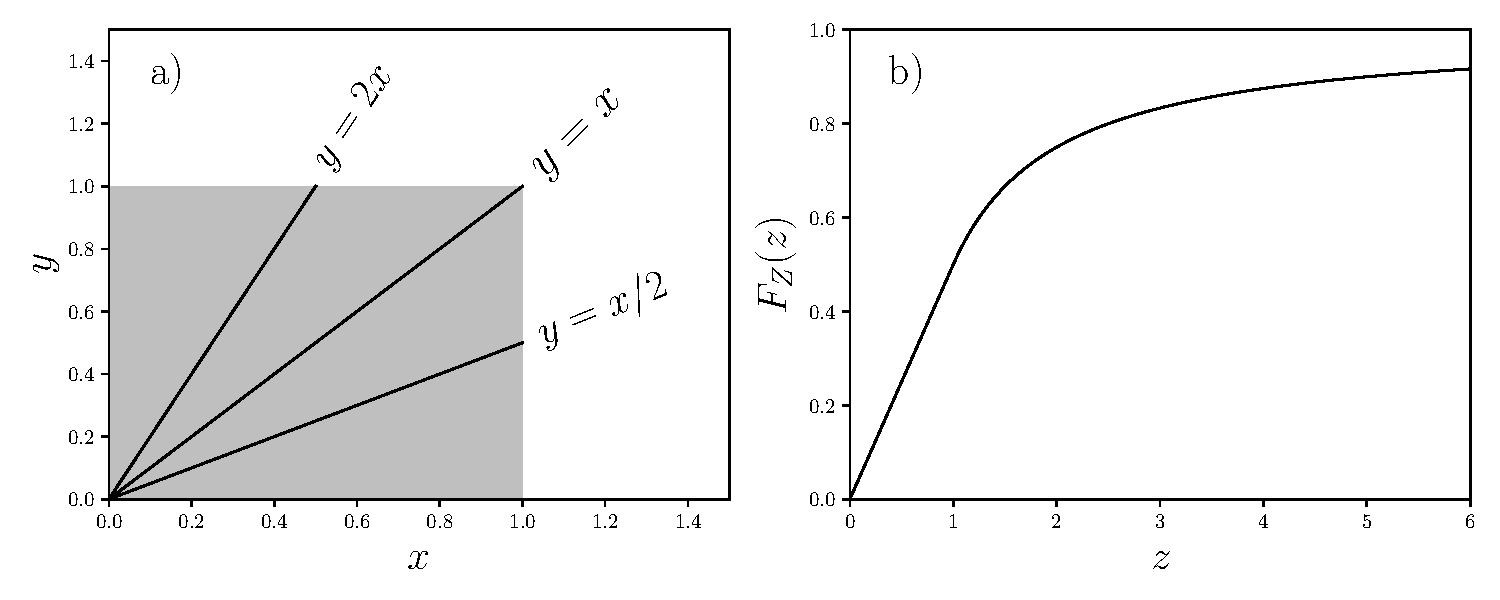
\includegraphics[totalheight=6cm]{chpt5/prob27.pdf}
  			  \caption{a) The $x-y$ plane where the shaded region denotes the region of non-zero probability for the PDF at hand.  b) A plot of the CDF of $Z$.}
    			   \label{fig:prob_27}
	\end{figure}
	
Continuing with the calculation:
\begin{align*}
F_Z(z) &=  \int_{0}^1 P\left(Y \ge \frac{x}{z}\right)dx,\\
& = \int_{0}^1 \int_{\min \{1, x/z \}}^1 f_Y(y)dy dx,\\
& = \int_0^1 \left [1- \min \left \{ 1, \frac{x}{z}\right \} \right]dx \\
& =1 - \int_0^1  \min \left \{ 1, \frac{x}{z}\right \} dx \\
& =1 - \left (\int_0^1 \mathbbm{1} \{x \ge z \}dx+\int_0^1\frac{x}{z} \mathbbm{1} \{x < z \}dx  \right),
\end{align*}
where I have picked out the proper value of the $\min$ function by utilizing an indicator function (which is much nicer to use in an integral since it ``kills" the integral whenever the logical condition evaluates to false).

Thus, for $z>1$ we have that:
\begin{align*}
F_Z(z) &=1 - \int_0^1 \frac{x}{z}dx \\
& =1-\frac{1}{2z},
\end{align*}
while for $z\in [0,1]$ we have that:
\begin{align*}
F_Z(z) &=1 - \left( \int_0^z \frac{x}{z}dx+\int_z^1 dx \right) \\
& =\frac{z}{2}.
\end{align*}
In summary we have:
\[
 F_Z(z) =
  \begin{cases}
                                  \frac{z}{2}& \text{for $0 \le z \le 1$} \\
                                   1 - \frac{1}{2z} & \text {for $z >1$} \\
                                   0& \text {otherwise},
   \end{cases}
\]
which I plot in Fig.~\ref{fig:prob_27} b).  Notice that even though this is a piecewise function, it appears very smooth because, at the transition ($z =1$), both the actual function and the first derivative match between the two piecewise regions.

To find the PDF we need only to differentiate:
\begin{align*}  
f_Z(z) &= \frac{dF_Z(z)}{dz} \\
& = \begin{cases}
                                  \frac{1}{2} &  \text{for $0 \le z \le 1$}\\
                                 \frac{1}{2z^2} &\text {for $z >1$} \\
                                 0& \text {otherwise}.
    \end{cases} \quad
\end{align*}


\end{problem}


\begin{problem}{28} $ $
\begin{enumerate}

\item  To find $f_{U|X}(x|u)$ I first solve for the conditional CDF then differentiate with respect to $u$:
\begin{align*}
F_{U|X}(u|x) &= P(U \le u |X=x) \\
& = P(X+Y \le u |X=x) \\
& = P(x+Y \le u |X=x) \\
& = P(Y \le u -x) \\
& = \Phi(u-x),
\end{align*}
where in the fourth line I have used the fact that $X$ and $Y$ are independent.  To find the conditional PDF I now differentiate:
\begin{align*}
\frac{\partial F_{U|X}}{\partial u} &=  \Phi^\prime(u-x) \\
 &=  \frac{1}{\sqrt{2 \pi}} e^{-\frac{(u-x)^2}{2}},
 \end{align*}
 and thus we see that:
 \begin{equation*}
 U|X=x \sim \mathcal N(x, 1).
 \end{equation*}
 
 \item If $X~\sim \mathcal N (\mu_x, \sigma_x^2)$ and $X~\sim \mathcal N (\mu_y, \sigma_y^2)$ are independent, then, as shown in the book by the method of convolution, $X+Y~\sim \mathcal N (\mu_x+\mu_y, \sigma_x^2+\sigma_y^2)$, and thus:
 \begin{equation*}
 U ~\sim \mathcal N(0, 2).
 \end{equation*}
 
 \item To find $f_{X|U}(x|u)$, I use Baye's rule for PDFs:
 \begin{align*}
f_{X|U}(x|u) & =\frac{f_{U|X}(u|x) f_X(x)}{f_U(u)}\\
& = \frac{\frac{1}{\sqrt{2\pi}} e^{-\frac{(u-x)^2}{2}} \frac{1}{\sqrt{2 \pi}} e^{-\frac{x^2}{2}} }{\frac{1}{2\sqrt{\pi}} e^{-\frac{u^2}{4}}} \\
& =\frac{1}{\sqrt{\pi}}e^{-\frac{(u-x)^2}{2} -\frac{x^2}{2}+\frac{u^2}{4}} \\
&=\frac{1}{\sqrt{\pi}} e^{-\left(x-\frac{u}{2}\right)^2} \\
&=\frac{1}{\sqrt{2 \pi} (1/\sqrt{2})} e^{-\frac{\left(x-\frac{u}{2}\right)^2}{2 \cdot \frac{1}{2}}},
 \end{align*}
 where I have used the ``completing the square" trick in the exponential to make it more Gaussian.  We recognize this distribution as a normal, $u/2$, $1/2$ distribution:
  \begin{equation*}
 X|U=u \sim \mathcal N\left (\frac{u}{2}, \frac{1}{2} \right).
 \end{equation*}

\item Since  $X|U=u \sim \mathcal N\left (\frac{u}{2}, \frac{1}{2} \right)$, we have:
\begin{equation*}
E[X|U=u] =\frac{u}{2},
\end{equation*}
and
\begin{equation*}
Var[X|U=u] =\frac{1}{2}.
\end{equation*}

\end{enumerate}
\end{problem}

\begin{problem}{29} This problem can be solved using the method of transformations.  Since $X$ and $Y$ are independent, we have an axis-aligned 2D Gaussian for the joint distribution:
\begin{align*}
f_{XY}(x,y) &= f_X(x)f_Y(y) \\
& = \frac{1}{ 2 \pi} e^{-\frac{1}{2}(x^2+y^2)}.
\end{align*}
I define the functions $h_1$ and $h_2$ as:
\[
\begin{cases}
               X = h_1(R, \Theta)= R\cos \Theta \\
	       Y = h_2(R, \Theta) = R\sin \Theta,
            \end{cases}
\]
so that, according to the method of transformations:
\begin{equation*}
f_{R\Theta}(r, \theta) = f_{XY}(h_1(r, \theta), h_2(r, \theta)) \begin{vmatrix}
\frac{\partial h_1}{\partial r} & \frac{\partial h_1}{\partial \theta}  \\ 
\frac{\partial h_2}{\partial r} & \frac{\partial h_2}{\partial \theta}
\end{vmatrix}.
\end{equation*}

The Jacobian is easy to calculate:
\begin{align*}
J &=  \begin{vmatrix}
\cos \theta & -r \sin \theta \\ 
\sin \theta & r\cos \theta 
\end{vmatrix}\\
& = r(\cos^2 \theta +\sin^2 \theta ) \\
& = r,
\end{align*}
where I have used the Pythagorean trigonometric identity.  Thus, we have that:
\begin{align*}
f_{R\Theta}(r, \theta) &= \frac{1}{2 \pi} e^{-\frac{(r \cos \theta)^2}{2}}e^{-\frac{(r \sin \theta)^2}{2}} r \\
&= \frac{r}{2 \pi} e^{-\frac{1}{2}r^2},
\end{align*}
where I have again used the Pythagorean trigonometric identity.

If $R$ and $\Theta$ are independent, then we can factor $f_{R\Theta}(r, \theta)$ into $f_{R}(r)f_\Theta(\theta)$.  To help determine what these 2 functions are, I integrate the joint distribution:
\begin{align*}
1 &=\int_0^\infty \int_{-\pi}^\pi f_{R\Theta}(r, \theta) dr d \theta \\
& =\int_0^\infty \int_{-\pi}^\pi \frac{r}{2 \pi} e^{-\frac{1}{2}r^2}dr d \theta \\
& = \int_0^\infty r e^{-\frac{1}{2}r^2}dr.
\end{align*}
Thus, we see that the function $r e^{-\frac{1}{2}r^2}$, which only depends on $r$, is always positive (for $r \ge 0$) and integrates to 1.  This is the marginal distribution of $R$.  The function $1/(2 \pi)$ is always positive and integrates to 1 for $\theta \in [-\pi, \pi]$, and this is thus the marginal distribution of $\Theta$.  Therefore we see that $f_{R\Theta}(r, \theta)$ can be factored into $f_{R}(r)f_\Theta(\theta)$, and thus $R$ and $\Theta$ are independent.



\end{problem}

\begin{problem}{30} If $X, Y\distas{iid} Unif(0, 1)$, then:
\[
 F_{XY}(x,y) =
  \begin{cases}
                                  1 & \text{for $x, y \in [0, 1]$} \\
                                   0 & \text {otherwise}.
   \end{cases}
\]
	\begin{figure}[t]
	\centering
      		 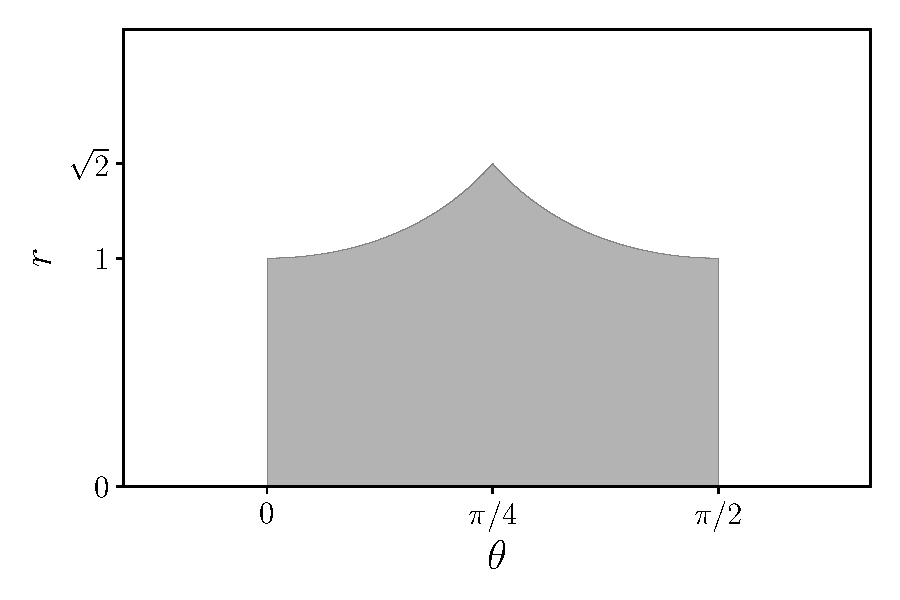
\includegraphics[totalheight=6cm]{chpt5/prob30b.pdf}
  			  \caption{The $r-\theta$ plane for Problem 30.  The grey region denotes the region in the plane where $f_{R\Theta}(r, \theta)$ is non-zero.}
    			   \label{fig:prob_30b}
	\end{figure}
The Jacobian has already been calculated in the previous problem ($J=r$), so that
\begin{align*}  
f_{R\Theta}(r, \theta) &= rF_{XY}(r\cos \theta ,r \sin \theta) \\
& = \begin{cases}
                                  r & \text{for $r\cos \theta ,r \sin \theta \in [0, 1]$} \\
                                   0 & \text {otherwise},
    \end{cases} \quad
\end{align*}
where in Fig.~\ref{fig:prob_30b}, I have indicated where in the $r-\theta$ plane $f_{R\Theta}(r, \theta)$ is non-zero.



We can further examine the constraints $r\cos \theta ,r \sin \theta \in [0, 1]$ to gain more insight.  Satisfying these conditions is equivalent to simultaneously satisfying the following four conditions:
\[
\begin{cases}
               r \cos \theta \le 1\\
               r \sin \theta \le 1\\
               r \cos \theta \ge 0\\
               r \sin \theta \ge 0.
            \end{cases}
\]
Since $r$ is always positive, the last 2 conditions yield $\cos \theta \ge 0 $ and $\sin \theta \ge 0$, which only happens in the first quadrant, i.e., $0 \le \theta \le \pi/2$.  If we plot the first 2 conditions for $0 \le \theta \le \pi/2$, as in Fig.~\ref{fig:prob_30}, we see that when $0 \le \theta \le \pi/4$, $r \cos \theta \le 1 \implies r \sin \theta \le 1$ and when $\pi/4 \le \theta \le \pi/2$, $r \sin \theta \le 1 \implies r \cos \theta \le 1$.

	\begin{figure}[t]
	\centering
      		 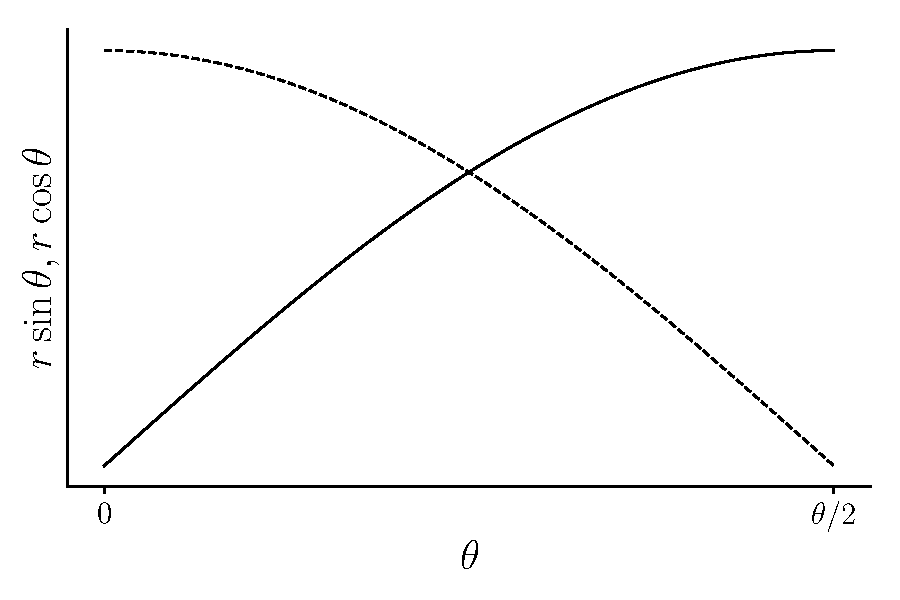
\includegraphics[totalheight=6cm]{chpt5/prob30.pdf}
  			  \caption{$r \sin \theta$ (solid line) and $r \cos \theta$ (dashed line) for $0 \le \theta \le \pi/2$}
    			   \label{fig:prob_30}
	\end{figure}
	
Thus, we can re-write $f_{R\Theta}(r, \theta)$ with the constraints specified a little more explicitly:
\[
 f_{R\Theta}(r, \theta) =
  \begin{cases}
                                  r & \text{for $0 \le \theta \le \frac{\pi}{4}$ and $r \le \frac{1}{\cos \theta}$}  \\
                                   r & \text{for $ \frac{\pi}{4} \le \theta \le \frac{\pi}{2}$ and $r \le \frac{1}{\sin \theta}$}  \\
                                    0 & \text {otherwise},
   \end{cases}
\]
(where the inequalities did not flip when I divided by $\cos \theta$ and $\sin \theta$ because these are both positive in the first quadrant). Note that these constraints imply that $f_{R\Theta}(r, \theta) >0 $ in the unit square and $f_{R\Theta}(r, \theta) =0 $ outside of the unit square, as we would expect for $X, Y \sim Unif(0,1)$ as shown in Fig.~\ref{fig:prob_30c}.  The figure shows the unit square in the $x-y$ plane (where the probability is non-zero), and it shows that for $\theta$ less than $\pi/4$, $r$ is constrained by $0\le r \le 1/ \cos \theta$ (for values of $r$ within the unit square).  One can similarly show in this figure that for $\theta $ greater than $\pi/4$, $0\le r \le 1/ \sin \theta$.

We can check explicitly that this PDF integrates to 1:
\begin{align*}
\int_0^{\frac{\pi}{4}} \int_0^{\frac{1}{\cos \theta}} r dr d\theta+\int_{\frac{\pi}{4}}^{\frac{\pi}{2}} \int_0^{\frac{1}{\sin \theta}} r dr d\theta &= \frac{1}{2}\int_0^{\frac{\pi}{4}}  \frac{1}{\cos^2 \theta}d\theta+\frac{1}{2}\int_{\frac{\pi}{4}}^{\frac{\pi}{2}}\frac{1}{\sin^2 \theta}d\theta \\
&=\frac{1}{2} \tan{\theta}\Big|_0^{\frac{\pi}{4}} -\frac{1}{2} \left(\frac{\cos \theta}{\sin \theta}\right )_{{\frac{\pi}{4}}}^{\frac{\pi}{2}} \\
&=1.
\end{align*}
For this problem $R$ and $\Theta$ are not independent, because there is no way to factor $f_{R\Theta}(r, \theta)$ into an equation of just $r$ times an equation of just $\theta$, since the values of $r$ over which the PDF is non-zero explicitly depend on the values of $\theta$.

	\begin{figure}[t]
	\centering
      		 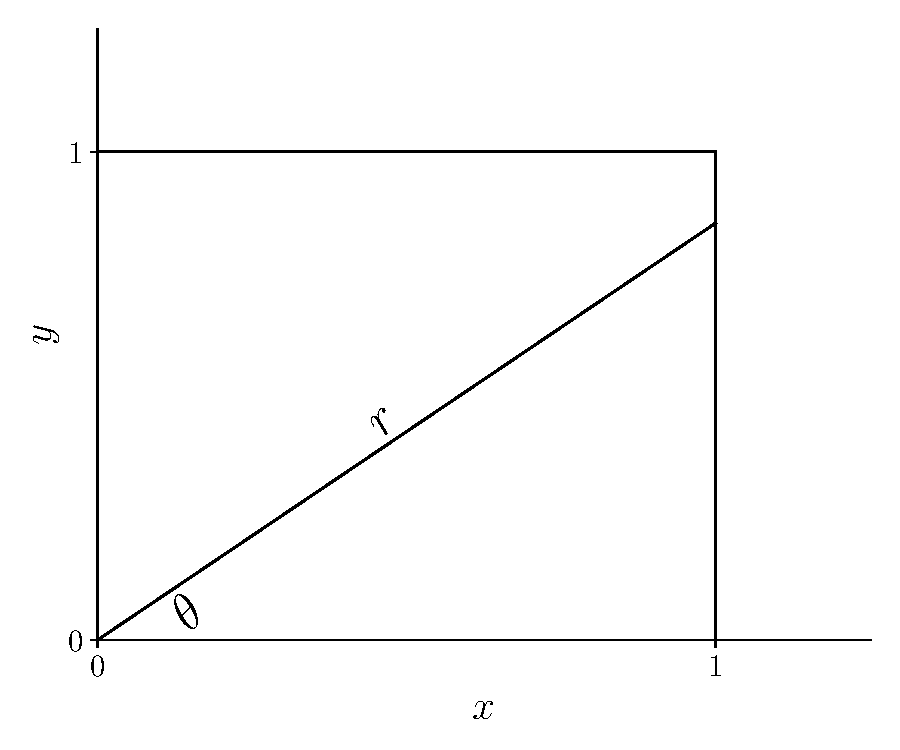
\includegraphics[totalheight=6cm]{chpt5/prob30c.pdf}
  			  \caption{The unit square in the $x-y$ plane.  In polar coordinates, to be within the unit square, it can be seen geometrically that $r$ is constrained by $0\le r \le 1/ \cos \theta$ for $0 \le \theta \le \pi/4$, and by $0\le r \le 1/ \sin \theta$ for $\pi/4< \theta \le \pi/2$.}
    			   \label{fig:prob_30c}
	\end{figure}

\end{problem}

\begin{problem}{31} The covariance can be computed straight from its definition:
\begin{align*}
Cov[X, Y] &= E[XY] -E[X]E[Y] \\
&= \sum_{x=0}^1 \sum_{y=0}^2 xy P_{XY}(x, y)-\left(\sum_{x=0}^1x P_X(x) \right) \left(  \sum_{y=0}^2y P_Y(y) \right) \\
& = 1\cdot \frac{1}{6}+2\cdot \frac{1}{6} -\left[1\cdot \left(\frac{1}{8}+\frac{1}{6}+\frac{1}{6}\right)\right]\left[1\cdot \left(\frac{1}{4}+\frac{1}{6}\right)+2\cdot \left(\frac{1}{8}+\frac{1}{6}\right) \right] \\
& = \frac{1}{24}.
\end{align*}

To calculate $\rho_{XY}$, I first calculate the variances.  For $X$ we have
\begin{equation*}
E[X] = \sum_{x=0}^1xP_X(x) = 1 \cdot \left (\frac{1}{8}+\frac{1}{6}+\frac{1}{6}\right) = \frac{11}{24},
\end{equation*}
\begin{equation*}
E[X^2] = \sum_{x=0}^1x^2P_X(x) = 1 \cdot \left (\frac{1}{8}+\frac{1}{6}+\frac{1}{6}\right) = \frac{11}{24} 
\end{equation*}
$\implies$
\begin{align*}
Var[X] &=E[X^2]-E[X]^2 \\
&=\frac{11}{24}- \left(\frac{11}{24} \right)^2 \\
&=\frac{143}{576},
\end{align*}
and for $Y$ we have
\begin{equation*}
E[Y] = \sum_{y=0}^2yP_Y(y) = 1 \cdot \left  (\frac{1}{4}+\frac{1}{6}\right)+2 \cdot \left (\frac{1}{8}+\frac{1}{6}\right) = 1,
\end{equation*}
\begin{equation*}
E[Y^2] = \sum_{y=0}^2y^2P_Y(y) = 1 \cdot \left (\frac{1}{4}+\frac{1}{6} \right)+2^2 \cdot \left (\frac{1}{8}+\frac{1}{6}\right) = \frac{19}{12}
\end{equation*}
$\implies$
\begin{align*}
Var[Y] &=E[Y^2]-E[Y]^2 \\
&=\frac{19}{12}- 1^2 \\
&=\frac{7}{12}.
\end{align*}
Finally, the correlation is:
\begin{equation}
\rho_{XY} = \frac{Cov[X, Y] }{\sqrt{Var[X] Var[Y]}} = \frac{\frac{1}{24}}{\sqrt{\frac{143}{576} \cdot \frac{7}{12}}} \approx 0.11.
\end{equation}
Thus, there is a weak, positive correlation between $X$ and $Y$.

\end{problem}

\begin{problem}{32} We can use several of the items in Lemma 5.3 in the book to solve this problem:
\begin{align*}
Cov[Z, W] &= Cov[11-X+X^2Y, 3-Y] \\
& = Cov[-X+X^2Y, -Y] \\
& = Cov[X, Y]-Cov[X^2Y, Y] \\
&=-Cov[X^2Y, Y] \\
& = -\left (E[X^2Y^2] -E[X^2Y]E[Y] \right ) \\
& = -\left (E[X^2]E[Y^2] -E[X^2]E[Y]^2 \right ) \\
& =-(1-0) \\
&=-1,
\end{align*}
where in the second line I have used item 5 of Lemma 5.3, in the third item 7, in the fourth item 2 in the sixth I have used the fact that $X$ and $Y$ are independent and in the seventh I have used the fact that $X, Y \sim \mathcal N(0,1)$.
\end{problem}

\begin{problem}{33} To solve this problem I use several of the items in Lemma 5.3 in the book.  Since $Z$ and $W$ are independent, we have that:
\begin{align*}
0 &= Cov[Z, W] \\
& = Cov[2X-Y, X+Y] \\
& = 2Cov[X, X]+2Cov[X, Y]-Cov[Y, X]-Cov[Y, Y] \\
& = 2 Var[X] +Cov[X, Y]-Var[Y] \\
& = 2 \cdot 4+ Cov[X, Y]- 9
\end{align*}
$\implies$
\begin{equation*}
Cov[X, Y] = 1.
\end{equation*}

The correlation is now straightforward to calculate: 
\begin{equation*}
\rho_{XY} = \frac{Cov[X, Y]}{\sqrt{Var[X] Var[Y]}} = \frac{1}{\sqrt{4 \cdot 9}} =\frac{1}{6}.
\end{equation*}


\end{problem}


\begin{problem}{34}
We know that $X \sim Unif(1, 3)$ (so that $E[X] = 2$) and $Y|X=x \sim Exp(x)$ (so that $E[Y|X] = 1/x$).  Since $Cov[X, Y] = E[XY]-E[X]E[Y]$, and since we know the distribution of $Y|X=x$ we can probably solve most of the expectations by conditioning on $X$ and using the law of iterated expectations.  To solve for $E[Y]$ I use the law of iterated expectations (where the subscript $X$ denotes an expectation over the random variable $X$):
\begin{align*}
E[Y] &= E_X[E[Y|X]] \\
 &= E_X\left [\frac{1}{X} \right ]\\
 &= \frac{1}{2}\int_1^3\frac{1}{x}dx \\
 & = \frac{1}{2} \ln 3.
\end{align*}
To solve for $E[XY]$ I also condition on $X$ and ``take out what is known":
\begin{align*}
E[XY] &= E_X[E[XY|X]] \\
 &= E_X[XE[Y|X]] \\
 &= E_X\left [X\frac{1}{X} \right] \\
 & = 1.
\end{align*}
Thus, we have that the covariance is:
\begin{align*}
Cov[X, Y] &= E[XY]-E[X]E[Y] \\
& = 1-2\cdot\frac{1}{2} \ln 3 \\
&= 1- \ln 3.
\end{align*}

\end{problem}

\begin{problem}{35} The covariance is:
\begin{align*}
Cov[Z, W] &= Cov[7+X+Y, 1+Y]\\
& = Cov[X+Y, Y]\\
& = Cov[X,Y]+Var[Y]\\
&= 0+1\\
&=1,
\end{align*}
where I have used the fact that $Cov[X,Y]=0$ since $X$ and $Y$ are independent. Calculating the variances is easy as well:
\begin{equation*}
Var[Z] = Var[7+X+Y] = Var[X]+Var[Y] = 2,
\end{equation*}
and
\begin{equation*}
Var[W] = Var[1+Y] = Var[Y] = 1.
\end{equation*}
Thus we have that the correlation is:
\begin{equation*}
\rho_{ZW} = \frac{Cov[Z, W]}{\sqrt{Var[Z] Var[W] }} = \frac{1}{\sqrt{2}} \approx 0.71.
\end{equation*}

\end{problem}

\begin{problem}{36} $ $
\begin{enumerate}
\item 
\begin{equation*}
X+2Y  \sim \mathcal N(\mu_X+2\mu_Y, \sigma_X^2+4\sigma_Y^2+2 \cdot 2 \rho \sigma_X \sigma_Y) =\mathcal N (1, 4)
\end{equation*}
$\implies$
\begin{equation*}
P(X+2Y \le 3) = \Phi \left (\frac{3-1}{2} \right)= \Phi (1) \approx 0.84.
\end{equation*}

\item

\begin{align*}
Cov[X-Y, X+2Y] & = Cov[X, X]+2 Cov[X, Y]-Cov[X, Y]-2 Cov[Y, Y] \\
& = \sigma_X^2+ \rho \sigma_X \sigma_Y -2 \sigma_Y^2 \\
& = 1
\end{align*}

\end{enumerate}
\end{problem}

\begin{problem}{37} $ $
\begin{enumerate}
\item 
\begin{equation*}
X+2Y  \sim \mathcal N(\mu_X+2\mu_Y, \sigma_X^2+4\sigma_Y^2+2 \cdot 2 \rho \sigma_X \sigma_Y) =\mathcal N (3, 8)
\end{equation*}
$\implies$
\begin{align*}
P(X+2Y > 4) &= 1-P(X+2Y \le 4) \\
& = 1 - \Phi \left (\frac{4-3}{\sqrt{8}} \right) \\
& = 1 - \Phi \left (\frac{1}{2\sqrt{2}} \right) \\
& \approx 0.36.
\end{align*}

\item Since $X$ and $Y$ are uncorrelated, jointly normal random variables they are independent, and thus:
\begin{align*}
E[X^2Y^2] &= E[X^2] E[Y^2] \\
&=(Var[X]+E[X]^2)(Var[Y]+E[Y]^2) \\
&=(\sigma_X^2+\mu_X^2)(\sigma_Y^2+\mu_Y^2) \\
&=10.
\end{align*}

\end{enumerate}
\end{problem}



\begin{problem}{38} $ $
\begin{enumerate}

\item $X$ and $Y$ are jointly normal random variables, and thus by Theorem 5.4 in the book:
\begin{align*}
Y|X=x &\sim \mathcal N \left (\mu_Y+\rho \sigma_Y \frac{x-\mu_X}{\sigma_X}, (1-\rho^2) \sigma_Y^2 \right) \\
&=\mathcal N \left(1-\frac{3(x-2)}{4}, \frac{27}{4} \right).
\end{align*}
We therefore can immediately read off that 
\begin{equation*}
E[Y|X=3] =1 -\frac{3(3-2)}{4} = \frac{1}{4}.
\end{equation*}

\item Using the same distribution:
\begin{equation*}
Var[Y|X=2] =\frac{27}{4}.
\end{equation*}

\item To solve for this problem, I define the random variables $U = X+2Y$ and $V=X+Y$ and I solve for the distribution of $U|V$.  Since $X$ and $Y$ are jointly normal random variables, so too are $U$ and $V$ (since $aU+bV = aX+2aY+bX+bY=(a+b)\cdot X+(2a+b)\cdot Y$ which we know is normal for all $a, b$) and thus Theorem 5.4 in the book gives an equation for the distribution of $U|V$.  But first to use this formula, we will need to explicitly compute the distributions of $U$ and $V$.  The distribution of $U$ is 
\begin{align*}
U &\sim \mathcal N(\mu_X+2\mu_Y, \sigma_X^2+4 \sigma_Y^2+2\cdot2\rho \sigma_X \sigma_Y) \\
& = \mathcal N(4, 28),
\end{align*}
and the distribution of $V$ is
\begin{align*}
V & \sim \mathcal N(\mu_X+\mu_Y, \sigma_X^2+\sigma_Y^2+2\rho \sigma_X \sigma_Y) \\
& = \mathcal N(3, 7).
\end{align*}
I will also need to compute $\rho_{UV}$, so I here solve for $Cov[U, V]$:
\begin{align*}
Cov[U, V] &= Cov[X+2Y, X+Y] \\
&=Cov[X, X]+Cov[X, Y]+2Cov[Y, X]+2Cov[Y, Y] \\
& = \sigma_X^2+3 \rho \sigma_X \sigma_Y+2 \sigma_Y^2 \\
&= 13.
\end{align*}
Thus, we have that:
\begin{equation*}
\rho_{UV} = \frac{Cov[U, V]}{\sqrt{Var[U] Var[V]}} = \frac{13}{\sqrt{28\cdot 7}} = \frac{13}{\sqrt{196}},
\end{equation*}
which, as a sanity check is in between -1 and 1.

Putting everything together into Theorem 5.4 in the book we have:
\begin{align*}
U|V=3 &\sim \mathcal N \left (\mu_U +\rho_{UV}\sigma_U \frac{3-\mu_V}{\sigma_V}, (1-\rho_{UV}^2)\sigma_U^2 \right)\\
&=\mathcal N \left (4, \left(1-\frac{13^2}{196}\right)\cdot 28 \right) \\
& = \mathcal N \left (4, \frac{27}{7} \right). 
\end{align*}
Finally, now that I have the distribution, I can compute the desired probability:
\begin{align*}
P(X+2Y \le 5|X+Y=3) &= P(U \le 5|V=3) \\
& = \Phi \left (\frac{5-4}{\sqrt{\frac{27}{7}}} \right) \\
& = \Phi \left(\sqrt{\frac{7}{27}} \right) \\
& \approx 0.69.
\end{align*}

\end{enumerate}
\end{problem}







\chapter{Methods for More Than Two Random Variables}
\begin{problem}{1} $ $

	\begin{enumerate}
		\item 
	\begin{align*}  
 f_{XY}(x, y) &= \int f_{XYZ}(x, y, z) dz \\ 
 &= \begin{cases}
                                 \int_0^1 (x+y) dz& \text{for $0\le x, y\le 1$} \\
                                  0& \text{otherwise}
       \end{cases} \\
&= \begin{cases}
                                 x+y & \text{for $0\le x, y\le 1$} \\
                                  0& \text{otherwise}
       \end{cases}
\end{align*}
		
\item
	
	\begin{align*}  
 f_{X}(x) &= \int f_{XY}(x, y) dy \\ 
 &= \begin{cases}
                                 \int_0^1 (x+y) dy& \text{for $0\le x\le 1$} \\
                                  0& \text{otherwise}
       \end{cases} \\
&= \begin{cases}
                                 x+\frac{1}{2} & \text{for $0\le x\le 1$} \\
                                  0& \text{otherwise}
       \end{cases}
\end{align*}
	
		
		
\item First note that:
	\begin{align*}  
 f_{Z}(z) &= \int f_{XYZ}(x, y, z) dx dy \\ 
 &= \begin{cases}
                                 \int_0^1 \int_0^1 (x+y) dx dy & \text{for $0\le z \le 1$} \\
                                  0& \text{otherwise}
       \end{cases} \\
&= \begin{cases}
                                 1& \text{for $0\le z\le 1$} \\
                                  0& \text{otherwise},
       \end{cases}
\end{align*}
so that \begin{equation*}
f_{XY|Z}(x, y|z) = \frac{f_{XYZ}(x, y, z)}{f_Z(z)} = f_{XYZ}(x, y, z).
\end{equation*}



\item

\begin{equation*}
f_{XY|Z}(x, y|z) = f_{XYZ}(x, y, z) = f_{XY}(x, y)
\end{equation*}
$\implies X$ and $Y$ are independent $Z$
\end{enumerate}

\end{problem}

\begin{problem}{2} $ $

Since $X$, $Y$, $Z$ are independent, $f_{XY|Z}(x, y|1) = f_{XY}(x, y) = f_X(x)f_Y(y)$, so that:
\begin{equation*}
E[XY|Z=1] = E[XY] = E[X]E[Y] = 0,
\end{equation*}
and
\begin{equation*}
E[X^2Y^2Z^2|Z=1] = E[X^2Y^2] = E[X^2]E[Y^2] = 1.
\end{equation*}

\end{problem}

\begin{problem}{3} $ $
To solve this problem, I first state a general result for a multivariate normal.  Suppose that 

\begin{equation*}
\begin{bmatrix} \bm{X_A} \\ \bm{X_B} \end{bmatrix} \sim \mathcal N \left(\begin{bmatrix} \bm{\mu_A} \\ \bm{\mu_B }\end{bmatrix},   \left[\begin{matrix}
    \bm{\Sigma_{AA}} & \bm{\Sigma_{AB}}\\
    \bm{\Sigma_{BA}} & \bm{\Sigma_{BB}}
\end{matrix}\right] \right),
\end{equation*}
where $\bm{X_A}, \bm{\mu_A} \in \mathbb R^{m}$, $\bm{X_B}, \bm{\mu_B} \in \mathbb R^{n}$, $\bm{\Sigma_{AA}} \in \mathbb R^{m\times m}$, $\bm{\Sigma_{BB}} \in \mathbb R^{n\times n}$, $\bm{\Sigma_{AB}} \in \mathbb R^{m\times n}$ and $\bm{\Sigma_{BA}} =\bm{\Sigma_{AB}}^T $.  (Note that, here, I have written this vector equation out in the so-called ``partitioned form" for convenience.)  Then, it is not difficult to show that\footnote{for example, see: Bishop, Christopher M. Pattern Recognition and Machine Learning. Springer,
2006.}:
\begin{equation*}
\bm{X_A}|\bm{X_B} = \bm{x_B} \sim \mathcal N (\bm{\mu_A}+\bm{\Sigma_{AB}} \bm{\Sigma_{BB}}^{-1}(\bm{x_B}-\bm{\mu_{B}}), \bm{\Sigma_{AA}}-\bm{\Sigma_{AB}}\bm{\Sigma_{BB}}^{-1}\bm{\Sigma_{BA}}).
\end{equation*}

I now define the random variable, $U = Y+Z$, solve for the joint PDF of $X, Y, U$, then condition on $U$ using the formula above so that I may compute $E[XY|Y+Z=1]$.  Since $U = Y+Z$, and $Y$ and $Z$ are 2 independent $\mathcal N (1, 1)$ distributions, then $U\sim \mathcal N (2, 2)$.  Recall that for 3 marginally normal distributions, the joint distribution is:
\begin{equation*}
\begin{bmatrix} X_1 \\ X_2 \\ X_3 \end{bmatrix} \sim \mathcal N \left(\begin{bmatrix} E[X_1] \\ E[X_2]\\ E[X_3] \end{bmatrix},   \left[\begin{matrix}
    Var[X_1] & Cov[X_1, X_2]& Cov[X_1, X_3] \\
    Cov[X_2, X_1] & Var[X_2] & Cov[X_2, X_3] \\
    Cov[X_3, X_1] & Cov[X_3, X_2]& Var[X_3]
\end{matrix}\right] \right).
\end{equation*}
Thus, to solve for the joint distribution of $X, Y, U$, all that is left to do is to calculate the covariance terms involving $U$, $Cov[U, X] = Cov[Y+Z, X] = 0$ and $Cov[U, Y] = Cov[Y+Z, Y] = Var[Y]$, so the the joint distribution is:
\begin{equation*}
\begin{bmatrix} X \\ Y \\ U \end{bmatrix} \sim \mathcal N \left(\begin{bmatrix} 1 \\ 1 \\ 2 \end{bmatrix},   \left[\begin{matrix}
    1 & 0 & 0\\
    0 & 1& 1 \\
    0 & 1 & 2
\end{matrix}\right] \right).
\end{equation*}
To solve for the distribution of $X, Y|U=1$, it is not difficult to identify that, here, $\bm{\Sigma_{AA}} = I_2$ (the $2\times 2$ identity matrix), $\bm{\Sigma_{AB}}=[0, 1]^T$, $\bm{\Sigma_{BA}}=[0, 1]$, and $\bm{\Sigma_{BB}}=2$, where I identify $\bm{X_A}$ with $[X, Y]^T$ and $\bm{X_B}$ with $U$.  The mean of the conditional distribution is therefore given by
\begin{equation*}
\bm{\mu_{A|B}} = \begin{bmatrix} 1 \\ 1 \end{bmatrix}+\begin{bmatrix} 0\\1 \end{bmatrix}\frac{1}{2}(1-2)=\begin{bmatrix} 1 \\ \frac{1}{2}\end{bmatrix},
\end{equation*}
and the covariance matrix of the conditional distribution is given by:
\begin{equation*}
\bm{\Sigma_{A|B}} =\left[\begin{matrix}
    1& 0\\
    0& 1 
\end{matrix}\right] -\left[\begin{matrix}
    0 \\
    1
\end{matrix}\right] \frac{1}{2}\left[\begin{matrix}
    0,1 
\end{matrix}\right] = \left[\begin{matrix}
1 & 0\\
0& \frac{1}{2}
\end{matrix}\right].
\end{equation*}
Finally, I have the conditional distribution I desire:
\begin{equation*}
X,Y|U=1 \sim \mathcal N \left(\begin{bmatrix} 1 \\ \frac{1}{2}\end{bmatrix},   \left[\begin{matrix}
1 & 0\\
0& \frac{1}{2}
\end{matrix}\right] \right).
\end{equation*}
We would like to solve for $E[XY|U=1]$, which we can get easily from the covariance term of the above distribution: $E[XY|U=1] = Cov[X, Y|U=1]+E[X|U=1]E[Y|U=1] = 0 +(1)\cdot (1/2) = 1/2$.

\end{problem}

\begin{problem}{4} $ $
Due to the symmetry of the problem, $Y_1, Y_2, \ldots Y_n$ are all identically distributed, and thus:
\begin{equation*}
E[Y] = E[Y_1+Y_2+\ldots +Y_n] = E[Y_1]+E[Y_2]+\ldots +E[Y_n]  = nE[Y_1],
\end{equation*}
and
\begin{equation*}
Var[Y] = Var[Y_1+Y_2+\ldots +Y_n] = \sum_{i=1}^n Var [Y_i]+2 \sum_{i<j} Cov[Y_i, Y_j]  = nVar[Y_1]+2 nCov[Y_1, Y_2].
\end{equation*}
The reason there is a factor of $n$ in front of the covariance term can be seen from the matrix below (an $n=5$ example).  The summation over $i<j$ means that we can only consider pairs of $i,j$ above the diagonal (shaded cells).  Further, it is evident that $Y_i, Y_j$ pairs that are 2 or more apart are independent.  For example, $Y_2=X_2X_3$, $Y_3=X_3X_4$, $Y_4=X_4X_5$, so that $Y_2$ and $Y_3$ are not independent because they share the $X_3$ random variable, but  $Y_2$ and $Y_4$ \textit{are} independent because they share no random variables (and all the $X_i$s are independent).  Since independence $\implies$ no covariance, the only $Y_i, Y_j$ pairs that contribute to the sum are the $n-1$ terms right above the diagonal (as indicated by the spades in the figure).  We also cannot forget that the $Y_n,Y_1$ pair is not independent because they share the $X_1$ random variable (the spade in the upper right hand corner).  We thus see that there are $n$ pairs that contribute to the sum.
\definecolor{light-gray}{gray}{0.70}
\begin{center}
\bgroup
\def\arraystretch{1.5}
  \begin{tabular}{ | c | c | c | c | c | c |}
    \hline
     & $Y_1$ & $Y_2$& $Y_3$& $Y_4$& $Y_5$ \\  \hline
    $Y_1$ &\cellcolor{light-gray} &$\spadesuit$ & & &$\spadesuit$ \\ \hline
    $Y_2$ & &\cellcolor{light-gray} &$\spadesuit$ && \\ \hline
    $Y_3$ & & &\cellcolor{light-gray} & $\spadesuit$ & \\ \hline
     $Y_4$ & & & &\cellcolor{light-gray} & $\spadesuit$\\ \hline
     $Y_5$ & & & & &\cellcolor{light-gray} \\
    \hline
  \end{tabular}
  \egroup
\end{center}

It remains to compute $E[Y_1]$, $Var[Y_1]$ and $Cov[Y_1, Y_2]$.  Since $Y_1 = X_1X_2$, and $X_1, X_2 \distas{iid} Bern(p)$, the range of $Y_1$ is $\{0, 1 \}$, with probability $p^2$ of obtaining $1$ ($X_1 =1$ and $X_2 = 1$).  In other words, $Y_1\sim Bern(p^2)$, so that $E[Y_1] = p^2$ and $Var[Y_1] = p^2 (1-p^2)$.  All that is left to do is to compute the covariance:
\begin{align*}
Cov[Y_1, Y_2] &= E[Y_1Y_2]-E[Y_1]E[Y_2] \\
&= E[X_1X_2 X_2X_3]-E[X_1X_2]E[X_2X_3] \\
& = E[X_1]E[X_2^2]E[X_3]-E[X_1]E[X_2]^2E[X_3] \\
& = p\cdot p \cdot p - p\cdot p^2 \cdot p \\
& = p^3(1-p),
\end{align*}
where in the second line I have used the fact that all the $X$s are independent, and in the fourth line I have used the fact that for a $Bern(p)$ distribution, $p(1-p) = E[X^2] - p^2$. 

Thus, we have that:
\begin{equation*}
E[Y]  = np^2
\end{equation*}
and
\begin{align*}
Var[Y] &= np^2(1-p^2)+2np^3(1-p) \\
& = np^2 (3p+1)(1-p).
\end{align*}

\end{problem}

\begin{problem}{5} $ $
\begin{enumerate}
\item To solve for the expectation, note that:
\begin{align*}
E[X] &= E[X_1+X_2+\ldots+X_k] \\
&= E[X_1]+E[X_2]+\ldots+E[X_k] \\
& = \sum_{j=0}^1 j P(X_1 = j)+\sum_{j=0}^1 j P(X_2 = j)+ \ldots+\sum_{j=0}^1 j P(X_k = j) \\
& = P(X_1 = 1)+ P(X_2 = 1)+ \ldots+P(X_k = 1),
\end{align*}
where in the second line I have used the linearity of expectation.  To solve this problem, we therefore need to solve for $P(X_i = 1)$ for all $i=1, 2, \ldots, k$.

To solve for $P(X_i = 1)$, first suppose that we draw all $b+r$ balls and create a specific sequence of blues and reds.  Note that all possible sequences are equally likely to occur. To see this, as an example, suppose $r=3$ and $b=2$ and we draw the sequence $RRBRB$.  The probability that this occurs is 
\begin{equation*}
\frac{3}{3+2}\cdot \frac{3-1}{3+2-1} \cdot \frac{2}{3+2-2} \cdot \frac{3-2}{3+2-3} \cdot \frac{2-1}{3+2-4} = \frac{3!2!}{(3+2)!}.
\end{equation*}
Suppose instead we had drawn the sequence $BRRBR$.  The probability that this sequence occurs is:
\begin{equation*}
\frac{2}{3+2}\cdot \frac{3}{3+2-1} \cdot \frac{3-1}{3+2-2} \cdot \frac{2-1}{3+2-3} \cdot \frac{3-2}{3+2-4} = \frac{3!2!}{(3+2)!}.
\end{equation*}

Notice that since the probability of all possible sequences with $r=3$ and $b=2$ is simply the product of the same terms in the numerators and the same terms in the denominators, but in a different order, the probability of any possible sequence is the same product.  Thus, in general, the probability of any specific sequence occurring is $r!b!/(b+r)!$.  As a check that all possible sequences are equally as likely and the probability of each sequence is $r!b!/(b+r)!$, if we multiply this probability by the total number of distinct sequences the result should be 1.  Taking into account the indistinguishability of all red balls and all blue balls, the total number of distinct sequences is $(b+r)!/(r!b!)$.  Multiplying these values together indeed results in 1.

Now that we know that all outcomes are equally as likely and that there is a finite sample space, we can use combinatorics to find the probabilities we are after.  Let us concentrate on the $i^{th}$ draw and compute the probability that the $i^{th}$ draw is blue.  Since all sequences are equally likely to occur, to compute this probability, we need only to divide the total number of unique sequences with a blue ball in the $i^{th}$ spot by the total number of possible unique sequences.  Since all red balls are indistinguishable and all blue balls are indistinguishable, as above, the total number of unique sequences is thus $(b+r)!/(r!b!)$.  The total number of unique sequences with a blue ball in the $i^{th}$ spot is $(b+r-1)!/[r!(b-1)!]$, and therefore the probability of obtaining a blue ball in the $i^{th}$ spot, $P(X_i=1)$, is:
\begin{equation*}
P(X_i=1) = \frac{\frac{(b+r-1)!}{r!(b-1)!}}{\frac{(b+r)!}{r!b!}} = \frac{b}{b+r}.
\end{equation*}

The desired expectation value is therefore 
\begin{align*}
E[X] &= P(X_1 = 1)+ P(X_2 = 1)+ \ldots+P(X_k = 1)\\
& = \underbrace{\frac{b}{b+r}+\frac{b}{b+r}+\ldots+\frac{b}{b+r}}_\text{$k$ times} \\
& = \frac{kb}{b+r}.
\end{align*}

\item To solve for $Var[X]$, I already have $E[X]$, so I just need to solve for $E[X^2]$:
\begin{align*}
E[X^2] &= E[(X_1+X_2+\ldots+X_k)^2] \\
& = E\left[\sum_{i=1}^kX_i^2+\sum_{i, j: i \neq j} X_iX_j \right] \\
& = \sum_{i=1}^kE[X_i^2]+\sum_{i, j: i \neq j} E[X_iX_j],
\end{align*}
where in the third line I have used the linearity of expectation, and where the notation $\sum_{i, j: i \neq j}$ refers to a summation over all $i,j$ pairs ($i,j$=1, 2, \ldots, k) expect the pairs for which $i=j$ (which was accounted for in the first summation).

We have already pretty much solved for $E[X_i^2]$:
\begin{align*}
 E[X_i^2]&= \sum_{j=0}^1 j^2 P(X_i = j) \\
 &= P(X_i = 1) \\
 &= \frac{b}{b+r}, 
 \end{align*}
 so that the first summation is:
\begin{equation*}
\sum_{i=1}^kE[X_i^2] = \frac{kb}{b+r}.
\end{equation*}
The second summation is slightly more difficult.  The strategy I take is to condition on one of the random variables and to use the law of total expectation (since $X_i, X_j \in \{ 0, 1\}$, so that one of the terms will go to zero):
\begin{align*}
E[X_iX_j] &= E[X_iX_j|X_j=0]P(X_j=0)+E[X_iX_j|X_j=1]P(X_j=1) \\
&= E[X_i|X_j=1]P(X_j=1) \\
& = \left[\sum_{l=0}^1 l P(X_i =l |X_j=1)\right ]P(X_j=1) \\
& = P(X_i=1|X_j=1)P(X_j=1),
\end{align*}
I thus need to solve for $P(X_i=1|X_j=1)$, which I can do in a very similar combinatorial fashion as I did for $P(X_i=1)$.  For this probability, the total sample space is all sequences of size $k$ with $b$ blue balls and $r$ red balls, with a blue ball in the $j^{th}$ spot.  The size of the sample space is thus $(b+r-1)!/[(b-1)!r!]$.  The number of unique sequences with a blue ball in the $j^{th}$ spot and a blue ball in the $i^{th}$ spot is $(b+r-2)!/[r!(b-2)!]$, so that 
\begin{equation*}
P(X_i=1|X_j=1) = \frac{\frac{(b+r-2)!}{r!(b-2)!}}{\frac{(b+r-1)!}{(b-1)!r!}} = \frac{b-1}{b+r-1}.
\end{equation*}
Finally, the second summation is 
\begin{align*}
\sum_{i, j: i \neq j} E[X_iX_j] &= \sum_{i, j: i \neq j}P(X_i=1|X_j=1)P(X_j=1) \\
& = \sum_{i, j: i \neq j}\frac{b-1}{b+r-1}\frac{b}{b+r} \\
& = \frac{(k^2-k)(b-1)}{b+r-1}\frac{b}{b+r},
\end{align*}
so that
\begin{align*}
 E[X^2] &= \frac{kb}{b+r}+\frac{(k^2-k)(b-1)}{b+r-1}\frac{b}{b+r} \\
 &=\frac{kbr+k^2b^2-bk^2}{(b+r)(b+r-1)}.
\end{align*}

The variance is thus:
\begin{align*}
Var[X] &= E[X^2] -E[X]^2 \\
& = \frac{kbr+k^2b^2-bk^2}{(b+r)(b+r-1)}-\left(\frac{kb}{b+r}\right)^2 \\
& = \frac{kbr(b+r-k)}{(b+r)^2(b+r-1)}.
\end{align*}


\end{enumerate}
\end{problem}


\begin{problem}{6} I start by writing out the definition of the MGF:
\begin{align*}
M_X(s) & = E[e^{sX}] \\
& = \sum_{k=1}^\infty p(1-p)^{k-1} e^{sk}\\
&= \frac{p}{1-p}\left  \{\sum_{k=0}^\infty[(1-p)e^{s}]^k-1\right \},
\end{align*}
where we recognize that the summation is a geometric series, and is finite provided $(1-p)e^{s}<1$.  Using the formula for a geometric series, and simplifying, I have that:
\begin{equation*}
M_X(s) =\frac{pe^{s}}{1+(p-1)e^s},
\end{equation*}
for $s< -\ln(1-p).$


\end{problem}

\begin{problem}{7}  We can solve this problem by realizing that the $k^{th}$ derivative of the MGF evaluated at $s=0$ gives the $k^{th}$ moment of the distribution:
\begin{align*}
E[X] &= \frac{dM_X}{ds}\Big |_{s=0} \\
&= \frac{d}{ds} \left [ \frac{1}{4}+\frac{1}{2}e^s+\frac{1}{4}e^{2s} \right] \bigg |_{s=0}  \\
& = 1,
\end{align*}
\begin{align*}
E[X^2] &= \frac{d^2M_X}{ds^2}\Big |_{s=0} \\
&= \frac{d^2}{ds^2} \left [ \frac{1}{4}+\frac{1}{2}e^s+\frac{1}{4}e^{2s} \right] \bigg |_{s=0}  \\
& = \frac{3}{2}.
\end{align*}
We therefore have that $Var[X] = 3/2-1^2 = 1/2.$

\end{problem}

\begin{problem}{8}  We already know from Problem 5 in section 6.1.6 of the book that the MGF for a $\mathcal N(\mu, \sigma^2)$ distribution is $M(s) = \exp ( s\mu +\sigma^2 s^2/2 )$, and since the MGF of the sum of independent random variables is the product of the MGFs of the random variables, we have that:
\begin{align*}
M_{X+Y}(s) &= M_X(s)M_Y(s) \\
&=\exp \left(s\mu_X+\frac{\sigma_X^2 s^2}{2} \right)\exp \left(s\mu_Y+\frac{\sigma_Y^2 s^2}{2} \right) \\
& = \exp \left[s(\mu_X+\mu_Y)+\frac{s^2}{2}(\sigma_X^2+\sigma_Y^2) \right].
\end{align*}
We recognize this as the MGF of a $\mathcal N(\mu_X+\mu_Y, \sigma_X^2+\sigma_Y^2)$ distribution.  Further, by Theorem 6.1 in the book, the MGF of a random variable uniquely determines its distribution, so that indeed $X+Y \sim \mathcal N(\mu_X+\mu_Y, \sigma_X^2+ \sigma_Y^2)$.

\end{problem}


\begin{problem}{9} As a note, for the Laplace distribution, $\lambda>0$.
\begin{align*}
M_X(s) &= E[e^{sX}] \\
& = \frac{\lambda}{2}\int_{-\infty}^\infty e^{-\lambda |x|+sx}dx \\ 
&=\frac{\lambda}{2}\left [\int_{-\infty}^0e^{x(\lambda+s)}dx+ \int_0^{\infty}e^{x(s-\lambda)}dx \right]
\end{align*}
Notice that, for both integrals to be finite, we have the conditions that $\lambda +s>0$ (for the first integral) and $s- \lambda <0$ (for the second), or in other words $|s|<\lambda$.  Assuming these two conditions, the integral can easily be evaluated, and is:
\begin{equation*}
M_X(s) = \frac{\lambda^2}{\lambda^2-s^2}.
\end{equation*}

\end{problem}

\begin{problem}{10}
\begin{align*}
M_X(s) &= E[e^{sX}] \\
& = \int_0^\infty \frac{e^{sx}\lambda^\alpha x^{\alpha-1}e^{-\lambda x}}{\Gamma(\alpha)}dx \\
& = \frac{\lambda^\alpha}{\Gamma(\alpha)}\int_0^\infty x^{\alpha-1} e^{-(\lambda-s)x}dx \\
&= \frac{\lambda^\alpha}{\Gamma(\alpha)}\frac{\Gamma(\alpha)}{(\lambda-s)^\alpha}~~\mathrm{for~} s<\lambda \\
& = \left( \frac{\lambda}{\lambda-s}\right)^\alpha
\end{align*}

\end{problem}


\begin{problem}{11} For $X_i \sim Exp(\lambda)$, from Example 6.5 in the book, we have that $M_{X_i} = \lambda/(\lambda-s)$ for $s<\lambda$.  Moreover since the MGF of the sum of independent random variables is the product of the MGFs of the random variables, we have that:
\begin{align*}
M_Y(s) &= M_{X_1}(s)M_{X_2}(s) \ldots M_{X_n}(s) \\
&=\left(\frac{\lambda}{\lambda-s}\right)^n,
\end{align*}
which, from the previous problem, we notice is the MGF of a $Gamma(n, \lambda)$ random variable.  By Theorem 6.1 in the book, the MGF of a random variable uniquely determines its distribution,
so $Y\sim Gamma(n, \lambda)$.
\end{problem}

\begin{problem}{12}
By the definition of the characteristic function, we have that:
\begin{align*}
\phi_Y(\omega) &= E[e^{i \omega Y}] \\
& = E[e^{i \omega (aX+b)}] \\
&= e^{i\omega b}E[e^{i(a\omega)X}] \\
&=e^{i\omega b}\phi_X(a\omega).
\end{align*}
\end{problem}

\begin{problem}{13}$ $
\begin{enumerate}
\item  To solve for $E[\bm U]$, I first find the marginal PDFs:
	\begin{equation*}  
 f_{X}(x) = \begin{cases}
                                  \int_0^1 \frac{1}{2}(3x+y)dy & \text{for $0\le x\le 1$} \\
                                  0& \text{otherwise}
       \end{cases} \\
= \begin{cases}
                                 \frac{3}{2}x+\frac{1}{4} & \text{for $0\le x\le 1$} \\
                                  0& \text{otherwise}
       \end{cases},
\end{equation*}
and
	\begin{equation*}  
 f_{Y}(y) = \begin{cases}
                                  \int_0^1 \frac{1}{2}(3x+y)dx & \text{for $0\le y\le 1$} \\
                                  0& \text{otherwise}
       \end{cases} \\
= \begin{cases}
                                 \frac{1}{2}y+\frac{3}{4} & \text{for $0\le y\le 1$} \\
                                  0& \text{otherwise}
       \end{cases}.
\end{equation*}
Thus, $E[X] = \int_0^1x(3x/2+1/4)dx = 5/8$ and $E[Y] = \int_0^1y(y/2+3/4)dy = 13/24$, so that
\begin{equation*}
E[\bm U]  =\begin{bmatrix} E[X] \\ E[Y] \end{bmatrix}= \left[\begin{matrix}
    \frac{5}{8}  \\[6pt]
    \frac{13}{24}
\end{matrix}\right].
\end{equation*}

\item In order to solve for$\bm R_U$, I will first need to compute $E[X^2]$, $E[Y^2]$ and $E[XY]$:
\begin{equation*}
E[X^2] = \int_0^1x^2 \left(\frac{3}{2}x+\frac{1}{4} \right)dx = \frac{11}{24},
\end{equation*}
\begin{equation*}
E[Y^2] = \int_0^1y^2 \left(\frac{1}{2}y+\frac{3}{4} \right)dy = \frac{3}{8},
\end{equation*}
and
\begin{equation*}
E[XY] = \frac{1}{2}\int_0^1 \int_0^1xy (3x+y)dxdy = \frac{1}{3}.
\end{equation*}
I can now immediately write down the correlation matrix:
\begin{align*}
\bm{R_U}  &= E[\bm U \bm U^T] \\
& = \left[\begin{matrix}
    E[X^2] & E[XY] \\
    E[YX] & E[Y^2] 
\end{matrix}\right] \\
&= \left[\begin{matrix}
    \frac{11}{24} & \frac{1}{3} \\[6pt]
    \frac{1}{3} & \frac{3}{8} 
\end{matrix}\right].
\end{align*}

\item  The covariance matrix is:

\begin{align*}
\bm{C_U}  &= E[\bm U \bm U^T]-E[\bm U] E[\bm U]^T \\
& =\bm{R_U} - \left[\begin{matrix}
    E[X]^2 & E[X]E[Y] \\
    E[Y]E[X] & E[Y]^2 
\end{matrix}\right] \\
&= \left[\begin{matrix}
    \frac{11}{24} & \frac{1}{3} \\[6pt]
    \frac{1}{3} & \frac{3}{8} 
\end{matrix}\right] -
 \left[\begin{matrix}
    \left(\frac{5}{8}\right)^2 & \left(\frac{5}{8}\right) \left(\frac{13}{24}\right) \\[6pt]
    \left(\frac{13}{24}\right)\left(\frac{5}{8}\right) & \left(\frac{13}{24}\right)^2 
\end{matrix}\right]  \\
&= \left[\begin{matrix}
    \frac{13}{192} & -\frac{1}{192} \\[6pt]
    -\frac{1}{192} & \frac{47}{576}
\end{matrix}\right].
\end{align*}

\end{enumerate}
\end{problem}



\begin{problem}{14}$ $

\begin{enumerate}
\item  First note that the range of $Y$ is $[0, 1]$.  Since we know the distribution of $Y|X=x$ and the distribution of $X$, the law of total probability for PDFs will probably be useful.  Note that $f_{Y|X}(y|x) = 1/x$ for $0 \le y \le x$ and 0 otherwise, which can be written as $(1/x)\mathbbm 1 \{0 \le y \le x \}$, which will be helpful in the integral to get the bounds of integration correct:
\begin{align*}
f_Y(y)& = \int_0^1 f_{Y|X}(y|x)f_X(x)dx \\
&= \int_0^1\frac{1}{x}\mathbbm 1 \{0 \le y \le x \} dx \\
&= \int_0^1\frac{1}{x}\mathbbm 1 \{y \le x \} dx ~~\mathrm{for~}y>0\\
&=\int_y^1\frac{1}{x} dx \\
&= - \ln y,
\end{align*}
and thus
\[
  f_Y(y) =
  \begin{cases}
                                   -\ln y & \text{for $0\le y\le1$} \\
                                   0 & \text{otherwise},
  \end{cases}
\]
which I checked integrates to 1. 

Finding the PDF of $Z$ is very similar to that of finding the PDF for $Y$.  Firstly, the range of $Z$ is $[0, 2]$.  Note that in this case $f_{Z|X}(z|x) = 1/2x$ for $0 \le z \le 2x$ and 0 otherwise, which can be written as $(1/2x)\mathbbm 1 \{0 \le z \le 2x \}$, so that the integral above becomes:
\begin{align*}
f_Z(z) &= \int_0^1\frac{1}{2x}\mathbbm 1 \{z \le 2x \} dx ~~\mathrm{for~}z>0\\
&=\int_{z/2}^1\frac{1}{2x} dx \\
&= \frac{\ln 2}{2}- \frac{\ln z}{2},
\end{align*}
and thus
\[
  f_Z(z) =
  \begin{cases}
                                   \frac{\ln 2}{2}- \frac{\ln z}{2} & \text{for $0\le z\le 2$} \\
                                   0 & \text{otherwise},
  \end{cases}
\]
which I checked integrates to 1. 

\item Using the chain rule of probability, we have that:
\begin{align*}
f_{XYZ}(x, y, z) &= f_{Z|XY}(z|x, y)f_{Y|X}(y|x)f_X(x) \\
& =f_{Z|X}(z|x)f_{Y|X}(y|x)f_X(x),
\end{align*}
where in the second line I used the fact that $Z$ and $Y$ are conditionally independent given $X$.  We thus have that 
\[
  f_{XYZ}(x, y, z) =
  \begin{cases}
                                   \frac{1}{2x^2} & \text{for $0\le x \le 1 $}, 0\le y \le x, 0\le z \le 2x \\
                                   0 & \text{otherwise},
  \end{cases}
\]
which I again checked integrates to 1. 
\end{enumerate}

\end{problem}


\begin{problem}{15}$ $
\begin{enumerate}

\item As stated in the problem, we have that 
\begin{equation*}
\begin{bmatrix} X_1 \\ X_2 \end{bmatrix} \sim \mathcal N \left(\begin{bmatrix} 1 \\ 2 \end{bmatrix},   \left[\begin{matrix}
    4 & 1 \\
    1 & 1 
\end{matrix}\right] \right),
\end{equation*}
and for a bivariate normal, we know that 
\begin{equation*}
\begin{bmatrix} X_1 \\ X_2 \end{bmatrix} \sim \mathcal N \left(\begin{bmatrix} E[X_1] \\ E[X_2] \end{bmatrix},   \left[\begin{matrix}
    Var[X_1] & Cov[X_1, X_2] \\
    Cov[X_2, X_1] & Var[X_2] 
\end{matrix}\right] \right).
\end{equation*}
Thus, I have that $X_2 \sim \mathcal N(2, 1)$, so that:
\begin{align*}
P(X_2>0) &= 1-P(X_2\le 0)\\
&= 1-\Phi \left(\frac{0-2}{1} \right) \\
&= \Phi(2) \\
& \approx 0.98.
\end{align*}

\item 

\begin{align*}
\bm Y &= \bm A \bm X +\bm b \\
=& \left[\begin{matrix}
    2 & 1 \\
    -1 & 1 \\
    1 & 3  
\end{matrix}\right] \begin{bmatrix} X_1 \\ X_2 \end{bmatrix}+\begin{bmatrix} -1 \\ 0 \\1 \end{bmatrix} \\
& = \begin{bmatrix} 2X_1+X_2-1 \\ -X_1+X_2 \\X_1+3X_2+1 \end{bmatrix}
\end{align*}
$\implies$
\begin{align*}
E[\bm Y] &=  \begin{bmatrix} 2E[X_1]+E[X_2]-1 \\ -E[X_1]+E[X_2] \\E[X_1]+3E[X_2]+1 \end{bmatrix}\\
& = \begin{bmatrix} 2\cdot 1+2-1 \\ -1+2 \\1+3\cdot 2+1 \end{bmatrix} \\
& = \begin{bmatrix} 3 \\ 1 \\8 \end{bmatrix} 
\end{align*}

\item  We know that a linear combination of a multivariate Gaussian random variable is also Gaussian.  Specifically, $\bm Y$ is distributed as $\bm Y\sim \mathcal N(\bm A E[\bm X] +\bm b, \bm A \bm{C_X} \bm A^T)$, and thus the covariance matrix of $\bm Y$ is
\begin{align*}
\bm{C_Y}& =  \bm A \bm{C_X} \bm A^T \\
&=\left[\begin{matrix}
    2 & 1 \\
    -1 & 1 \\
    1 & 3  
\end{matrix}\right] \left[\begin{matrix}
    4 & 1 \\
    1 & 1
\end{matrix}\right] \left[\begin{matrix}
    2 & -1 &1 \\
    1 & 1 & 3 
\end{matrix}\right] \\
& = \left[\begin{matrix}
    21& -6 &18 \\
    -6& 3 & -13 \\
    18& -3 &19 
\end{matrix}\right].
\end{align*}
Notice that, as it should be, $\bm{C_Y}$ is symmetric.

\item As with the first part of this problem, we know that

\begin{equation*}
\begin{bmatrix} Y_1 \\Y_2 \\Y_3 \end{bmatrix} \sim \mathcal N \left(\begin{bmatrix} E[Y_1] \\ E[Y_2]  \\ E[Y_3] \end{bmatrix},   \left[\begin{matrix}
    Var[Y_1] & Cov[Y_1, Y_2] & Cov[Y_1, Y_3] \\
    Cov[Y_2, Y_1] & Var[Y_2] & Cov[Y_2, Y_3] \\
    Cov[Y_3, Y_1] & Cov[Y_3, Y_2] & Var[Y_3]
\end{matrix}\right] \right),
\end{equation*}
so that $Y_2 \sim \mathcal N(1, 3)$, and therefore:
\begin{equation*}
P(Y_2 \le 2) = \Phi \left(\frac{2-1}{\sqrt{3}} \right) \approx 0.72.
\end{equation*}

\end{enumerate}

\end{problem}

\begin{problem}{16}  To solve this problem, I first review how to ``complete the square" for matrices.  For $a \in \mathbb R$, $x, b \in \mathbb R^{m}$ and $C \in \mathbb R^{m \times m}$ (and symmetric), a quadratic of the form
\begin{equation*}
a+{\bm b}^T{\bm x} + \frac{1}{2}{\bm x}^T \bm C {\bm x}
\end{equation*}
can be factored into the form
\begin{equation*}
\frac{1}{2}({\bm x}-{\bm m})^T \bm M ({\bm x}-{\bm m})+v,
\end{equation*}
where 
\begin{equation*}
\bm M= \bm C,
\end{equation*}
\begin{equation*}
{\bm m}=-\bm C^{-1}{\bm b},
\end{equation*}
and
\begin{equation*}
v = a-\frac{1}{2} {\bm b}^T \bm C^{-1} {\bm b}.
\end{equation*}
I now explicitly write out the MGF of $\bm X$:
\begin{align*}
M_{\bm X}(s, t, r) &= E[e^{sX_1+tX_2+rX_3}] \\
& = \int_{\mathbb R^3} \exp \{ \bm s^T \bm x \}\frac{1}{(2 \pi)^{3/2} |\bm \Sigma|^{1/2}} \exp \left \{-\frac{1}{2}(\bm x-\bm \mu)^T \bm \Sigma^{-1}(\bm x-\bm \mu) \right \}d^3x\\
& =\frac{1}{(2 \pi)^{3/2} |\bm \Sigma|^{1/2}} \int_{\mathbb R^3}  \exp \left \{ -\frac{1}{2}(\bm x-\bm \mu)^T \bm \Sigma^{-1}(\bm x-\bm \mu) + \bm s^T \bm x\right \}d^3x,
\end{align*}
where $\bm x^T \equiv [x_1, x_2, x_3]$ and $\bm s^T \equiv[s, t, r]$.  To make the exponent more Gaussian looking, I now expand the exponent out and complete the square (note that since $\bm \Sigma$ is symmetric, then so too is $\bm \Sigma^{-1}$):
\begin{align*}
-\frac{1}{2}(\bm x-\bm \mu)^T \bm \Sigma^{-1}(\bm x-\bm \mu) + \bm s^T \bm x & = -\frac{1}{2}\left [ \bm x^T \bm \Sigma^{-1}\bm x -\bm x^T \bm \Sigma^{-1}\bm \mu-\bm \mu^T \bm \Sigma^{-1}\bm x  +\bm \mu^T \bm \Sigma^{-1}\bm \mu  \right ] + \bm s^T \bm x \\
 & = -\frac{1}{2} \bm x^T \bm \Sigma^{-1}\bm x +\bm \mu^T \bm \Sigma^{-1}\bm x  -\frac{1}{2} \bm \mu^T \bm \Sigma^{-1}\bm \mu + \bm s^T \bm x \\
  & = -\frac{1}{2} \bm x^T \bm \Sigma^{-1}\bm x +(\bm s^T+ \bm \mu^T \bm \Sigma^{-1})\bm x  -\frac{1}{2} \bm \mu^T \bm \Sigma^{-1}\bm \mu,
\end{align*}
where I have used the fact that $(\bm x^T \bm \Sigma^{-1}\bm \mu )^T=\bm x^T \bm \Sigma^{-1}\bm \mu$ since this is just a real number.  I can now read off $a$, $\bm b$ and $\bm C$:
\begin{equation*}
a = -\frac{1}{2} \bm \mu^T \bm \Sigma^{-1}\bm \mu,
\end{equation*}
\begin{equation*}
\bm b^T = \bm s^T+ \bm \mu^T \bm \Sigma^{-1}
\end{equation*}
and 
\begin{equation*}
\bm C = -\bm \Sigma^{-1},
\end{equation*}
so that 
\begin{equation*}
\bm b =(\bm b ^T)^T =\bm s + \bm \Sigma^{-1} \bm \mu
\end{equation*}
and 
\begin{equation*}
\bm C^{-1} = \left( -{\bm  \Sigma^{-1}}\right)^{-1}=-\bm \Sigma .
\end{equation*} 
Finally, the exponent can be re-expressed as
\begin{equation*}
-\frac{1}{2}({\bm x}-{\bm{\tilde m}})^T \bm {\tilde M }({\bm x}-{{\bm{\tilde m}}})+\tilde v,
\end{equation*}
where 
\begin{equation*}
\bm{\tilde m} = \bm \Sigma(\bm s+\bm \Sigma^{-1}\bm \mu),
\end{equation*}
\begin{equation*}
\bm{\tilde M} = \bm \Sigma^{-1}
\end{equation*}
and
\begin{align*}
\tilde v &= -\frac{1}{2} \bm \mu^T \bm \Sigma^{-1}\bm \mu +\frac{1}{2}(\bm s^T+ \bm \mu^T \bm \Sigma^{-1}) \bm \Sigma (\bm s + \bm \Sigma^{-1} \bm \mu) \\
& =\bm s^T \bm \mu +\frac{\bm s^T \bm \Sigma s}{2},
\end{align*}
so that the integral becomes:
\begin{align*}
M_{\bm X}(s, t, r) &= \exp ( \tilde v) \frac{1}{(2 \pi)^{3/2} | \bm \Sigma |^{1/2}} \int_{\mathbb R^3}  \exp \left \{ -\frac{1}{2}({\bm x}-{\bm{\tilde m}})^T \bm \Sigma^{-1}({\bm x}-{{\bm{\tilde m}}})\right \}d^3x \\
&=\exp \left ( \bm s^T \bm \mu +\frac{\bm s^T \bm \Sigma s}{2} \right ) ~~ \forall \bm s \in \mathbb R^3.
\end{align*}
I have used the fact that the integral is that of a Gaussian integrated over its entire domain, so that the integral evaluates to 1.  Note that we probably could have guessed this form of the MGF of $\bm X$, since it is the vector analogue of the 1 dimensional case: $M_X(s) = \exp \{s\mu +\sigma^2 s^2/2 \}$, as found in Problem 5 of 6.1.6 in the book.

The specified values of the mean vector and covariance matrix are:
\begin{equation*}
 \bm \mu = \left[\begin{matrix}
    1\\
    2 \\
    0
\end{matrix}\right],
\end{equation*}
and 
\begin{equation*}
\bm \Sigma = \left[\begin{matrix}
    9& 1 &-1 \\
    1& 4 & 2 \\
    -1& 2 &4
\end{matrix}\right],
\end{equation*}
and plugging in these specific values into the equation I derived above, and multiplying the matrices, I finally arrive at:
\begin{equation*}
M_{\bm X}(s, t, r) = \exp \left \{ s\left (\frac{9}{2}s+1 \right)+2t(t+1)+2r^2-rs+st+2rt \right \}.
\end{equation*}

\end{problem}

\begin{problem}{17}  Let $A_i$, $i=1, 2, 3, 4$, be the event that the $i^{th}$ component fails, so that the a failure occurs under the event $\cup_{1=i}^4A_i$.  We can thus obtain an upper limit on the event that failure occurs using the union bound:
\begin{align*}
P\left(\bigcup_{1=i}^4A_i\right) & \le \sum_{i=1}^4P(A_i) \\
& \le 4 p_f \\
&=\frac{1}{25}.
\end{align*}

\end{problem}

\begin{problem}{18} $ $
\begin{enumerate}

\item First note that for the random position of a node $(X_i, Y_i)$, $X_1, X_2, \ldots, X_n, Y_1, Y_2, \ldots, Y_n \distas{iid} Unif(0, 1)$.  Let us call the node under consideration node $j$, and let the set $\mathcal S$ be defined as $\mathcal S \equiv \{1, 2, \ldots, n \}-\{j\}$.  The probability that the node is isolated, $p_d$, is:

\begin{align*}
p_d &= P\left(\bigcap_{i \in \mathcal S}\left  [(X_j-X_i)^2+(Y_j-Y_i)^2>r^2 \right] \right) \\
& = \int_0^1 \int_0^1 P\left(\bigcap_{i \in \mathcal S}\left  [(X_i-X_j)^2+(Y_i-Y_j)^2>r^2 \right]  \Big |X_j=x_j, Y_j=y_j\right)f_{X_jYj}(x_j,y_j) dx_j dy_j \\
& = \int_0^1 \int_0^1 P\left(\bigcap_{i \in \mathcal S}\left  [(X_i-x_j)^2+(Y_i-y_j)^2>r^2 \right]  \right)f_{X_j}(x_j) f_{Y_j}(y_j) dx_j dy_j \\
& =  \int_0^1 \int_0^1 \prod_{i \in \mathcal S} P\left((X_i-x_j)^2+(Y_i-y_j)^2>r^2  \right)f_{X_j}(x_j) f_{Y_j}(y_j) dx_j dy_j \\
& =  \int_0^1 \int_0^1 \prod_{i \in \mathcal S} \left[1-P\left((X_i-x_j)^2+(Y_i-y_j)^2 \le r^2  \right)\right]f_{X_j}(x_j) f_{Y_j}(y_j) dx_j dy_j \\
& =  \int_0^1 \int_0^1 \left[1-P\left((X_1-x_j)^2+(Y_1-y_j)^2 \le r^2  \right)\right]^{n-1} f_{X_j}(x_j) f_{Y_j}(y_j) dx_j dy_j,
\end{align*}
where in the third and fourth lines I have used the fact that the random variables are independent, and in the last line, I have used symmetry.  I now must compute $P((X_1-x_j)^2+(Y_1-y_j)^2 \le r^2 )$.  If the given point $(x_j, y_j)$ is near the middle of the square (as in the upper point in Fig.~\ref{fig:prob_18}) then the probability of this event is simply the area of this circle (shaded grey region).  However, we notice that if $(x_j, y_j)$ is near the edge of the square, part of the shaded circle will get cutoff.  In fact, if $(x_j, y_j)$ is exactly at one of the corners of the unit square, for example, at $(0,0)$ as in Fig.~\ref{fig:prob_18}, then the amount of shaded area is minimized at $\pi r^2/4$.  Thus, for any given $(x_j, y_j)$, $P((X_1-x_j)^2+(Y_1-y_j)^2 \le r^2 ) \ge \pi r^2/4$.  Therefore,
\begin{align*}
p_d & \le \int_0^1 \int_0^1 \left(1-\frac{\pi r^2}{4}\right)^{n-1} f_{X_j}(x_j) f_{Y_j}(y_j) dx_j dy_j \\
&= \left(1-\frac{\pi r^2}{4}\right)^{n-1}
\end{align*}

	\begin{figure}[t]
	\centering
      		 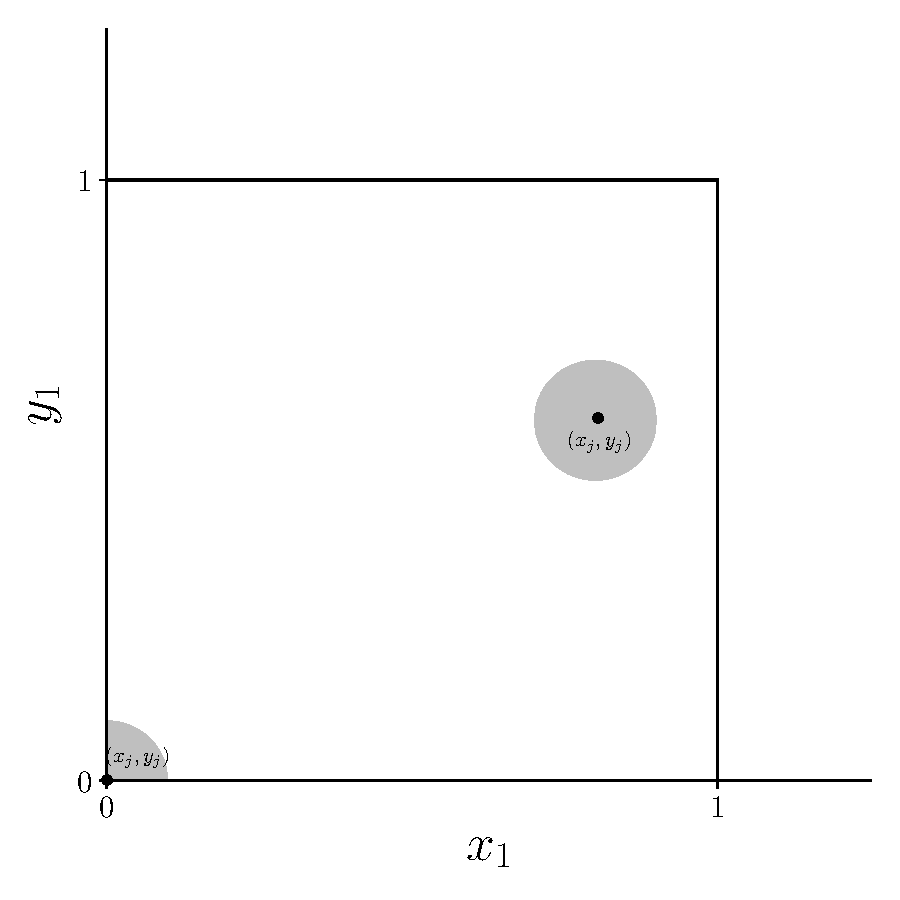
\includegraphics[totalheight=10cm]{chpt6/prob18.pdf}
  			  \caption{Two example nodes at $(x_j, y_j)$ for Problem 18.}
    			   \label{fig:prob_18}
	\end{figure}

\item Let $A_i$ be the event that the $i^{th}$ node is isolated.  Then the probability we seek is:
\begin{align*}
P\left(\bigcup_{i=1}^n A_i \right) & \le \sum_{i=1}^n P(A_i) \\
& = \sum_{i=1}^n p_d \\
& = n \left(1-\frac{\pi r^2}{4}\right)^{n-1}
\end{align*}

\end{enumerate}

\end{problem}

\begin{problem}{19}  For $X\sim Geom(p)$, $E[X] = 1/p$, so that the Markov inequality is:
\begin{equation*}
P(X \ge a) \le \frac{E[X]}{a} = \frac{1}{pa}.
\end{equation*}
The exact probability is:
\begin{align*}
P(X \ge a) &= \sum_{k=a}^\infty p(1-p)^{k-1}\\
& = \frac{p}{1-p}\left(\sum_{k=0}^\infty (1-p)^{k}-\sum_{k=0}^{a-1} (1-p)^{k} \right) \\
& = \frac{p}{1-p}\left(\frac{1}{1-(1-p)}-\frac{1-(1-p)^a}{1-(1-p)}\right) \\
&=(1-p)^{a-1}.
\end{align*}
The Markov upper bound is greater than or equal to the exact probability for $a \ge 1$ and $0<p<1$ as shown for a few values of $a$ in Fig.~\ref{fig:prob_19}

	\begin{figure}[t]
	\centering
      		 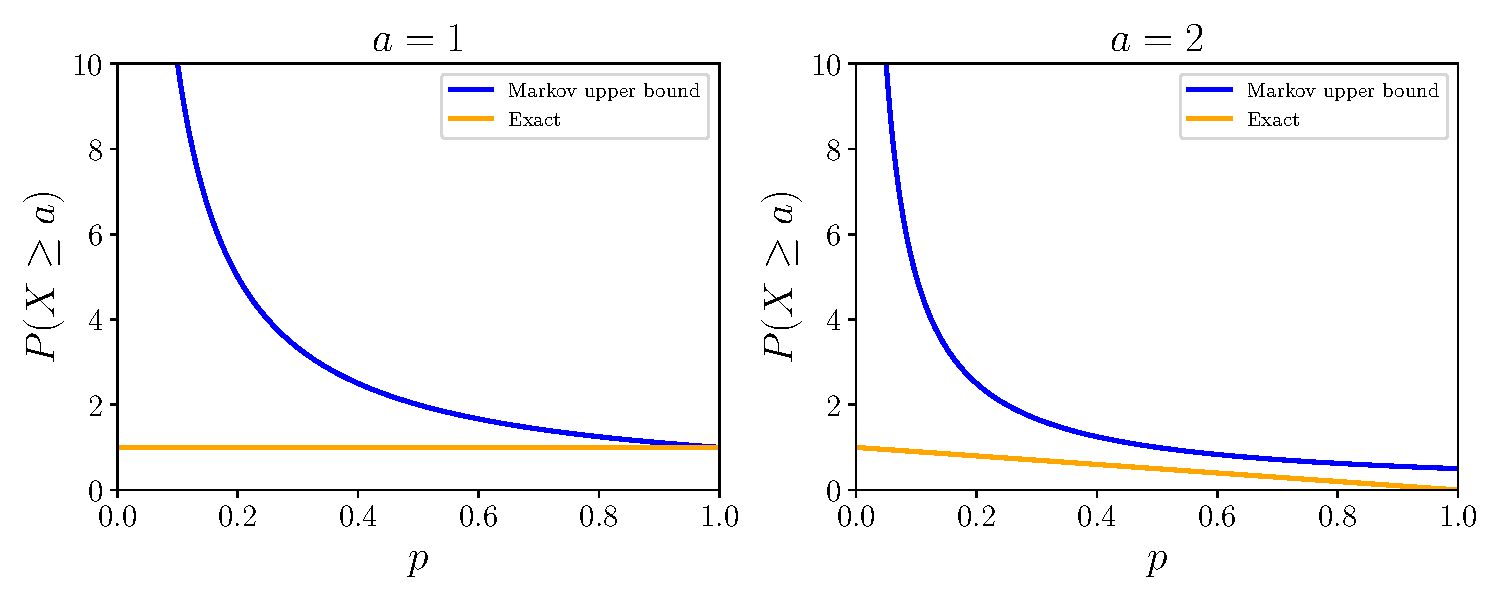
\includegraphics[totalheight=6cm]{chpt6/prob19.pdf}
  			  \caption{Comparison of Markov upper bound to exact probability for Problem 19.}
    			   \label{fig:prob_19}
	\end{figure}
\end{problem}

\begin{problem}{20}

\begin{equation*}
P(|X-E[X]|\ge b)\le \frac{Var[X]}{b^2} = \frac{1-p}{pb^2}
\end{equation*}

\end{problem}

\begin{problem}{21}
\begin{align*}
P(X \ge a) &= P\left(X+\frac{\sigma^2}{a} \ge a+\frac{\sigma^2}{a}\right) \\
&=P\left(\left(X+\frac{\sigma^2}{a}\right)^2 \ge \left (a+\frac{\sigma^2}{a} \right)^2\right) \\
& \le \frac{E\left[(X+\frac{\sigma^2}{a})^2\right]}{\left(a+\frac{\sigma^2}{a}\right)^2}~~\mathrm{Markov's~Inequality} \\
&=\frac{\sigma^2+\frac{\sigma^4}{a^2}}{a^2(1+\frac{\sigma^2}{a^2})^2} \\
& = \frac{\sigma^2}{a^2+\sigma^2}
\end{align*}

\end{problem}

\begin{problem}{22}$ $
\begin{enumerate}

\item 
\begin{align*}
P(X\le 80 \mathrm{~or~} X \ge 120) &= P(|X-100|\ge 20) \\
& = P(|X-E[X]|\ge 20) \\
& \le \frac{225}{20^2}~~ \mathrm{by~Chebyshev} \\
& = \frac{9}{16}
\end{align*}

\item
\begin{equation*}
P(X \ge 120) \le \frac{225}{225+120^2} =\frac{45}{293}
\end{equation*}

\end{enumerate}

\end{problem}

\begin{problem}{23}
We know from Problem 11 that if $X_1, X_2, \ldots, X_n\distas{iid} Exp(\lambda)$, then $Y\equiv X_1+X_2+\ldots+X_n\sim Gamma(n, \lambda)$.  The relevant Chernoff bound is given by:
\begin{equation*}
P(Y \ge a) \le \min_{s>0} \{ e^{-sa}M_X(s) \},
\end{equation*}
where, in this case the $M_X(s)$ is the MGF for a $Gamma(n, \lambda)$ distribution.  This MGF was solved for in Problem 10, and is given by
\begin{equation*}
M_X(s) = \left(\frac{\lambda}{\lambda-s}\right)^n~~\mathrm{for}~s<\lambda,
\end{equation*}
and therefore we must minimize the objective function over $0<s<\lambda$.  Let the optimal value be called $s^\star$.  I solve for $s^\star$ in the standard calculus manner by setting the derivative equal 0.  I then check to make sure that this optimal value is within the interval $(0, \lambda)$.  The derivative of the objective can be found easily with the chain rule:
\begin{equation*}
\frac{d}{ds} e^{-sa} \left(\frac{\lambda}{\lambda-s}\right)^n = -a e^{-sa} \left(\frac{\lambda}{\lambda-s}\right)^n+ne^{-sa}\left(\frac{\lambda}{\lambda-s}\right)^n\frac{1}{\lambda-s},
\end{equation*}
and setting this equal to zero and solve for $s^\star$ results in
\begin{equation*}
s^\star = \lambda - \frac{n}{a}.
\end{equation*}
As stipulated in the problem $a>n/\lambda$, which means that $n/a$ is positive and less than $\lambda$.  Thus we have that $s^\star \in (0, \lambda)$ as required.

The desired bound is therefore
\begin{align*}
P(Y\ge a) & \le e^{-s^{\star}}M_X(s^\star) \\
& = e^{-\lambda a +n}\left(\frac{\lambda a}{n} \right)^n.
\end{align*}

We can understand the behavior of this function as $n \rightarrow \infty$ by expanding the exponential in powers of $1/n$:
\begin{align*}
e^{-\lambda a +n}\left(\frac{\lambda a}{n} \right)^n &= e^{-\lambda a} \left[1 +\mathcal{O}\left(\frac{1}{n}\right) \right]\left(\frac{1}{n} \right)^n(\lambda a )^n \\
& = e^{-\lambda a} \left(\frac{\lambda a }{n} \right)^n+\mathcal{O}\left (\left(\frac{1}{n}\right)^{n+1} \right),
\end{align*}
and we thus see that the upper bound goes to 0 exponentially fast as $n$ goes to infinity.


\end{problem}

\begin{problem}{24}
Using some properties of absolute values I have that:
\begin{align*}
E[|X+Y|^{p-1}|X|] &= E[|(X+Y)^{p-1}| |X|] \\
& =E[|(X+Y)^{p-1}X|]\\
& \le E[|(X+Y)^{p-1}|^{\frac{p}{p-1}}]^{\frac{p-1}{p}}E[|X|^p]^{\frac{1}{p}}\\
&=E[|X+Y|^p]^{\frac{p-1}{p}}[|X|^p]^{\frac{1}{p}},
\end{align*}
where in the third line I have used H{\"o}lder's inequality, $E[|UV|] \le E[|U|^\alpha]^{1/\alpha}E[|V|^\beta]^{1/\beta}$, with $1<\alpha, \beta< \infty$ and $1/\alpha+1/\beta=1$, and where I have specifically chosen $\alpha=p/(p-1)$ and $\beta=p$.

Using the inequality provided in the book,
\begin{align*}
E[|X+Y|^p] & \le E[|X+Y|^{p-1}|X|] +E[|X+Y|^{p-1}|Y|] \\ 
& \le E[|X+Y|^p]^{\frac{p-1}{p}}(E[|X|^p]^{\frac{1}{p}}+E[|Y|^p]^{\frac{1}{p}}),
\end{align*}
and multiplying both sides of this equation by $E[|X+Y|^p]^{(1-p/p)}$ (which we can do without flipping the inequality sign since we know that this quantity is positive) yields the desired result:
\begin{equation*}
E[|X+Y|^p] ^{\frac{1}{p}}\le E[|X|^p]^{\frac{1}{p}}+E[|Y|^p]^{\frac{1}{p}}.
\end{equation*}

\end{problem}


\begin{problem}{25}$ $
\begin{enumerate}
\item 
\begin{equation*}
\frac{d^2}{dx^2}(x-x^3) = -6x
\end{equation*}
$\implies$ 
\[
  g^{\prime \prime}(x) =
  \begin{cases}
                                   +~\text{(convex)}& \text{for $x<0$} \\
                                   -~\text{(concave)} &  \text{for $x>0$} ,
  \end{cases}
\]
Since we know $X$ is a positive random variable, by Jensen's inequality, we have:
\begin{equation*}
E[X-X^3] \le E[X]-E[X]^3 = -990.
\end{equation*}

\item

\begin{equation*}
\frac{d^2}{dx^2}(x\ln \sqrt{x}) = \frac{1}{2x}
\end{equation*}
$\implies$ 
$ g^{\prime \prime}(x)>0$ (convex) for $x>0$
$\implies$ 
\begin{equation*}
E[X\ln \sqrt{X}] \ge E[X]\ln \sqrt{E[X]}= 10 \ln \sqrt{10}
\end{equation*}

\item  The function is a typical absolute value function, an upward v shape hitting $y=0$ at $x=2$, which is clearly convex, since a straight line drawn from any 2 points on the graph is always above the graph.  Therefore, I have that $E[|2-X|]\ge |2-E[X]| = 8.$
\end{enumerate}

\end{problem}

\begin{problem}{26} Taking the second derivative, we have that $d^2/dx^2 (x^3-6x^2) = 6x-12$.  Setting to zero and solving for $x$, I find that the second derivative is negative for $x<2$ and positive for $x>2$.  Since the range of $X$ is $(0,2)$, we have that $g(x) = x^3-6x^2$ is concave in this interval.  By Jensen's inequality, this implies that $E[Y] = E[g(X)] \le g(E[X]) = E[X]^3-6E[X]^2 = 1-6 = -5$.

\end{problem}



\chapter{Limit Theorems and Convergence of Random Variables}
\begin{problem}{1}$ $
\begin{enumerate}
\item 
\begin{align*}
E[M_n] &= \frac{1}{n}E[X_1+\ldots+X_n] \\
& = \frac{1}{n}nE[X_1] \\
& = \frac{1}{2}
\end{align*}

\begin{align*}
Var[M_n] &= \frac{1}{n^2}Var[X_1+\ldots+X_n] \\
& = \frac{1}{n^2}nVar[X_1] ~~\mathrm{(independence)}\\
& = \frac{1}{12n}
\end{align*}

\item 
\begin{align*}
P\left(\left |M_n-\frac{1}{2} \right| \ge \frac{1}{100}\right) &= P\left( |M_n-E[M_n]| \ge \frac{1}{100}\right) \\
& \le \frac{Var[M_n]}{\left(\frac{1}{100}\right)^2} \\
& = \frac{2500}{3n}
\end{align*}

\item

\begin{equation*}
\lim_{n \rightarrow \infty} P\left( |M_n-E[M_n]| \ge \frac{1}{100}\right)\le \lim_{n \rightarrow \infty} \frac{2500}{3n} = 0
\end{equation*}
$\implies$
\begin{equation*}
\lim_{n \rightarrow \infty} P\left( \left|M_n-\frac{1}{2}\right| \ge \frac{1}{100}\right) = 0
\end{equation*}

\end{enumerate}
\end{problem}

\begin{problem}{2} Let $X_1, X_2, \ldots, X_{365}$ be the number of accidents on day 1, day 2, $\ldots$, day 365, so that the total number of accidents in the year is $Y = X_1+\ldots+X_{365}$.  We know that $X_1, X_2, \ldots, X_{365} \distas{iid} Poiss(\lambda)$, where $\lambda = $ 10 accidents/day, so that $\mu = E[X_i] = \lambda = 10$ and $\sigma = \sqrt{Var[X_i]} = \sqrt{\lambda} = \sqrt{10}$.   Using the central limit theorem, I have
\begin{align*}
P(Y>3800) & = P\left(\frac{Y-365\cdot 10}{\sqrt{365\cdot 10}}>\frac{3800-365\cdot 10}{\sqrt{365\cdot 10}} \right) \\
& = P\left(Z_{365}>\frac{3800-365\cdot 10}{\sqrt{365\cdot 10}} \right) \\
& = 1- P\left(Z_{365} \le \frac{3800-365\cdot 10}{\sqrt{365\cdot 10}} \right) \\
& \approx 1- \Phi \left( \frac{3800-365\cdot 10}{\sqrt{365\cdot 10}}\right ) \\
& \approx 6.5 \times 10^{-3}.
\end{align*}
\end{problem}

\begin{problem}{3} Let the random variable, $X_i$ be 0 if the $i^{th}$ bit is not received in error and 1 if it is.  Notice that $X_1, X_2, \ldots, X_{1000} \distas{iid} Bern(0.1)$, and let the total number of errors, $Y$, be $Y=X_1+\ldots+X_{1000}$.  Note that $\mu = E[X_i] = p = 0.1$ and $\sigma = \sqrt{Var[X_i]} = \sqrt{p(1-p)} = \sqrt{0.09}$.  We seek the probability of decoding failure, in other words $P(Y>125)$:
\begin{align*}
P(Y>125) &= 1- P(Y \le125) \\
& = 1- P\left (\frac{Y-1000\cdot 0.1}{\sqrt{0.09\cdot 1000}} \le \frac{125-1000\cdot 0.1}{\sqrt{0.09\cdot 1000}}\right ) \\
& = 1- P\left (Z_{1000} \le \frac{125-1000\cdot 0.1}{\sqrt{0.09\cdot 1000}}\right ) \\
& \approx 1- \Phi \left(\frac{25}{3\sqrt{10}} \right)\\
&= 4.2 \times 10^{-3}.
\end{align*}

\end{problem}

\begin{problem}{4} Let the random variable, $X_i$ be 0 if the $i^{th}$ student does not have a car and 1 if the $i^{th}$ student does have a car.  Notice that $X_1, X_2, \ldots, X_{50} \distas{iid} Bern(0.5)$, and let the total number of cars, $Y$, be $Y=X_1+\ldots+X_{50}$.  Note that $\mu = E[X_i] = p = 0.5$ and $\sigma = \sqrt{Var[X_i]} = \sqrt{p(1-p)} = 0.5$.  We seek the probability that there are not enough car spaces, in other words $P(Y>30)$:
\begin{align*}
P(Y>30) &= P(Y>29.5)~~\mathrm{(using~the~continuity~correction)} \\
&=1- P(Y \le 29.5) \\
& = 1- P\left (\frac{Y-50\cdot 0.5}{\sqrt{50}\cdot 0.5} \le \frac{29.5-50\cdot 0.5}{\sqrt{50}\cdot 0.5}\right ) \\
& = 1- P\left (Z_{50} \le \frac{29.5-50\cdot 0.5}{\sqrt{50}\cdot 0.5}\right ) \\
& \approx 1- \Phi \left(1.27 \right)\\
& \approx 0.10.
\end{align*}

\end{problem}

\begin{problem}{5} Let $N$, a random variable, be the number of jobs processed in 7 hours (420 mins).  We seek the probability that the number of jobs processed in 7 hours is less than or equal to 40, $P(N\le 40)$.  This can be rephrased as the probability that the total time to processes 40 jobs is greater than or equal to 7 hours:
\begin{align*}
P(N\le 40) &= P(X_1+\ldots+X_{40} \ge 420) \\
& = P\left(\frac{X_1+\ldots+X_{40}-40\cdot 10}{\sqrt{40}\cdot \sqrt{2}} \ge \frac{420-40\cdot 10}{\sqrt{40}\cdot \sqrt{2}} \right) \\
& = P\left(Z_{40} \ge \frac{5}{\sqrt{5}}\right) \\
& = 1 - P\left(Z_{40} < \frac{5}{\sqrt{5}}\right) \\
& \approx 1 - \Phi \left(\frac{5}{\sqrt{5}}\right) \\
& \approx 1.3 \times 10^{-2}.
\end{align*}

\end{problem}

\begin{problem}{6} Let $X_i$ be the number of heads flipped on toss $i$, so that the total proportion of heads out of $n$ tosses, $X$, is $X=(X_1+ \ldots +X_n)/n$.  Notice that $X_1, \ldots, X_n \distas{iid}Bern(0.5)$, so that $\mu = E[X_i] = p = 0.5$ and $\sigma = \sqrt{Var[X_i]} = \sqrt{0.5^2} = 0.5$.  To be at least 95\% sure that $0.45\le X \le 0.55$, we have that:
\begin{align*}
0.95 & \le P(0.45 \le X \le 0.55) \\
& = P\left(\frac{0.45n-n\cdot0.5}{\sqrt{n}\cdot 0.5} \le \frac{X_1+\ldots+X_n-n\cdot0.5}{\sqrt{n}\cdot 0.5} \le \frac{0.55n-n\cdot0.5}{\sqrt{n}\cdot 0.5} \right) \\
& = P\left(-0.1 \sqrt{n} \le Z_n \le 0.1 \sqrt{n}  \right) \\
& \approx \Phi (0.1 \sqrt{n}) - \Phi (-0.1 \sqrt{n}) \\
& =2\Phi (0.1 \sqrt{n}) - 1.
\end{align*}
Thus, I have that $0.95 \lesssim 2 \Phi(0.1\sqrt{n})-1$.  Applying the inverse normal CDF function to this inequality, I arrive at:
\begin{equation}
n \gtrsim \ceil*{100\left[ \Phi^{-1} \left ( \frac{1.95}{2} \right)\right]^2} = 385.
\end{equation}

\end{problem}

\begin{problem}{7} Note that $X_1, X_2, \ldots, X_n$ are $iid$ with $\mu = E[X_i] = 0$ and $\sigma = \sqrt{Var[X_i]} = 2$, so we can use the CLT.  To be at least 95\% sure that the final estimate is within 0.1 units of $q$, we require:
\begin{align*}
0.95 &\le P(q-0.1 \le M_n \le q+0.1) \\
& = P \left (q-0.1 \le \frac{X_1+\ldots+X_n +nq}{n} \le q+0.1 \right) \\
& = P \left ((q-0.1)n-nq \le X_1+\ldots+X_n \le (q+0.1)n-nq \right) \\
& = P \left (\frac{(q-0.1)n-nq}{2\sqrt{n}} \le \frac{X_1+\ldots+X_n}{2\sqrt{n}} \le \frac{(q+0.1)n-nq}{2\sqrt{n}} \right) \\
& = P \left (\frac{-0.1\sqrt{n}}{2} \le Z_n \le \frac{0.1\sqrt{n}}{2} \right) \\
& \approx \Phi \left( \frac{0.1\sqrt{n}}{2} \right)-\Phi \left( \frac{-0.1\sqrt{n}}{2} \right) \\
& = 2\Phi \left( \frac{0.1\sqrt{n}}{2} \right)-1.
\end{align*}
We therefore have that $0.95 \lesssim 2 \Phi(0.1\sqrt{n}/2)-1$.  Applying the inverse normal CDF function to this inequality, I arrive at:
\begin{equation}
n \gtrsim \ceil*{400\left[ \Phi^{-1} \left ( \frac{1.95}{2} \right)\right]^2} = 1537.
\end{equation}
\end{problem}

\begin{problem}{8}  To solve this problem, I first compute the limit of $\exp[n(x-1)]/\{1+\exp[n(x-1)] \}$ for $x>0$ as $n$ goes to $\infty$.  Notice that this function has different behavior for $x=1$ (in which case the limit evaluates easily to 1/2), $0<x<1$ (in which case the limit evaluates easily to 0) and for $x>1$ (in which case the numerator and denominator evaluate to infinity).  Using L'hopital's rule in this case I find that the limit evaluates to 1.  Therefore, I have that:
\begin{equation*}  
\lim_{n \rightarrow \infty} F_{X_n}(x) = \begin{cases}
                                   \lim_{n \rightarrow \infty} \frac{e^{n(x-1)}}{1+e^{n(x-1)}} & \text{for $x > 0$} \\
                                   0& \text{otherwise} 
       \end{cases} \quad
= \begin{cases}
                                   0 & \text{for $-\infty<x<1$} \\
                                    \frac{1}{2} & \text{for $x = 1$} \\
                                   1 & \text{for $x >1$}.
       \end{cases}
\end{equation*}
For the ``random variable", $X$, that takes on a value of 1 with probability 1, the CDF is:
\[
  F_X(x) =
  \begin{cases}
                                   0 & \text{for $-\infty<x<1$} \\
                                   1 & \text{for $x\ge1$}
  \end{cases}
\]
Thus, we see that $\lim_{n \rightarrow \infty} F_{X_n}(x)= F_X(x)$ everywhere $F_X(x)$ is continuous (i.e, $\mathbb{R}-\{1\}$), and hence $X_n \xrightarrow{d} X$.

\end{problem}

\begin{problem}{9}  To solve this problem, I first state without proof the following 2 limits:
\begin{equation*}
\lim_{n\rightarrow \infty}\frac{e^{nx}+xe^{nx}}{1+\left(\frac{n+1}{n}\right) e^n} = x~~~\mathrm{for}~~0\le x \le1,
\end{equation*}
and
\begin{equation*}
\lim_{n\rightarrow \infty}\frac{e^{nx}+e^{nx}}{1+\left(\frac{n+1}{n}\right) e^n} = 1~~~\mathrm{for}~~x>1.
\end{equation*}
I therefore have that:
\begin{equation*}  
\lim_{n \rightarrow \infty} F_{X_n}(x) = \begin{cases}
				0 & \text{for $x < 0$} \\
                                  \lim_{n\rightarrow \infty}\frac{e^{nx}+xe^{nx}}{1+\left(\frac{n+1}{n}\right) e^n} & \text{for $0\le x \le 1$} \\
                                   \lim_{n\rightarrow \infty}\frac{e^{nx}+e^{nx}}{1+\left(\frac{n+1}{n}\right) e^n}& \text{for $x>1$} 
       \end{cases} \quad
= \begin{cases}
                                   0 & \text{for $x < 0$} \\
                                   x & \text{for $0\le x \le 1$}\\
                                   1 & \text{for $x >1$},
\end{cases}
\end{equation*}
which is the same CDF as a $Unif(0,1)$ distribution.  Hence, $X_n \xrightarrow{d} X$ for $X\sim Unif(0,1)$.

\end{problem}

\begin{problem}{10} $ $
\begin{enumerate}

\item 

\begin{align*}
\lim_{n \rightarrow \infty}P(|X_n-0|\ge \epsilon) &= \lim_{n \rightarrow \infty}P(X_n\ge \epsilon) ~~(\mathrm{since}~X_n\ge 0) \\
& = \begin{cases}
                                   \frac{1}{n^2} & \text{for $\epsilon \le n$} \\
                                    0 & \text{for $\epsilon >n$}
       \end{cases}\\
& = \lim_{n \rightarrow \infty} \frac{1}{n^2} \\
& = 0
\end{align*}

$\implies X_n \xrightarrow{p} 0$

\item 

\begin{align*}
\lim_{n \rightarrow \infty}E[|X_n-0|^r] &= \lim_{n \rightarrow \infty}E[X_n^r] ~~(\mathrm{since}~X_n\ge 0) \\
& = \lim_{n \rightarrow \infty} \frac{1}{n^2}n^r \\
& = \lim_{n \rightarrow \infty} n^{r-2} \\
& = 0 ~~(\mathrm{for}~1\le r<2) 
\end{align*}
$\implies X_n \xrightarrow{L^r} 0$ (for $1\le r<2$)

\item 
For $r \ge 2$,
\begin{align*}
\lim_{n \rightarrow \infty}E[|X_n-0|^r] &= \lim_{n \rightarrow \infty}E[X_n^r] ~~(\mathrm{since}~X_n\ge 0) \\
& = \lim_{n \rightarrow \infty} \frac{1}{n^2}n^r \\
& = \lim_{n \rightarrow \infty} n^{r-2},
\end{align*}
which converges to 1 for $r=2$ and diverges for $r>2$.  Therefore, $X_n$ does not converge to 0 in the $r^{th}$ mean for $r \ge 2$.

\item  To solve this problem I use Theorem 7.5 in the book, and must thus show that $\sum_{n=1}^\infty P(|X_n| > \epsilon)$ (for all $\epsilon>0$) is finite:
\begin{align*}
\sum_{n=1}^\infty P(|X_n|> \epsilon)& =\sum_{n=1}^\infty P(X_n> \epsilon) \\
& = \sum_{n=\ceil{\epsilon}}^\infty \frac{1}{n^2} \\
&\le \sum_{n=1}^\infty \frac{1}{n^2} \\
& = \frac{\pi^2}{6} \\
& < \infty,
\end{align*}
where in the first line I have used the fact that $X_n$ is always greater than or equal to zero.

\end{enumerate}
\end{problem}

\begin{problem}{11} $ $
This is a hypergeometric experiment with $b = n+\delta$ (with $\delta = 0, 1, 2, \ldots$), $r=n$ and $k=10$, so that the PMF for $X_{10}, X_{11}, \ldots$ is given by:
\begin{equation*}
P_{X_n}(x) = \frac{\binom{n+\delta}{x}\binom{n}{10-x}}{\binom{2n+\delta}{10}},
\end{equation*}
for $x = 0, 1, \ldots 10$ (and 0 otherwise).  Since $X, X_{10}, X_{11}, \ldots$ are non-negative random integers (for $X\sim Bin(10, 0.5)$), by Theorem 7.1 in the book, we need only prove that $\lim_{n \rightarrow \infty}P_{X_n}(x) = P_X(x)$ to prove convergence in distribution.  As for the RHS of this equation, for $X\sim Bin(10, 0.5)$, the PMF is given by:
\begin{equation*}
P_{X}(x) = \binom{10}{x}(0.5)^{10},
\end{equation*}
for $x=0, 1, \ldots, 10$ (and 0 otherwise).   

As for the LHS of this equation, taking the limit of $P_{X_n}(x)$ as $n \rightarrow \infty$ I have that:
\begin{align*}
\lim_{n \rightarrow \infty}P_{X_n}(x) &= \lim_{n \rightarrow \infty} \frac{\binom{n+\delta}{x}\binom{n}{10-x}}{\binom{2n+\delta}{10}} \\
& = \lim_{n \rightarrow \infty} \binom{n+\delta}{x} \lim_{n \rightarrow \infty} \binom{n}{10-x}  \left[\lim_{n \rightarrow \infty} \binom{2n+\delta}{10}\right]^{-1}.
\end{align*}
The first limit can be found easily by expanding the factorial in the numerator:
\begin{align*}
\lim_{n \rightarrow \infty} \binom{n+\delta}{x} &= \frac{1}{x!}\lim_{n \rightarrow \infty} (n+\delta)(n+\delta-1)\ldots(n+\delta-x+1) \\
&=\frac{1}{x!}\lim_{n \rightarrow \infty} n^x + \mathcal{O}\left( n^{x-1}\right) \\
& = \lim_{n \rightarrow \infty} \frac{n^x}{x!},
\end{align*}
and the remaining 2 limits can be worked out similarly.  Plugging these limits in, I have that:
\begin{align*}
\lim_{n \rightarrow \infty}P_{X_n}(x) &= \lim_{n \rightarrow \infty} \left \{ \frac{n^x}{x!} \right \} \lim_{n \rightarrow \infty} \left \{ \frac{n^{10-x}}{(10-x)!} \right \} \lim_{n \rightarrow \infty}  \left \{ \left[\frac{(2n)^{10}}{10!} \right] \right \}^{-1}\\
&= \lim_{n \rightarrow \infty}\left \{ \frac{n^x}{x!} \cdot \frac{n^{10-x}}{(10-x)!} \cdot \left[\frac{(2n)^{10}}{10!} \right]^{-1} \right \} \\
& = \binom{10}{x}(0.5)^{10}.
\end{align*}
Thus $\lim_{n \rightarrow \infty}P_{X_n}(x) = P_X(x)$, and by Theorem 7.1 $X_{n} \xrightarrow{d} X$.

\end{problem}

\begin{problem}{12} Let 
\begin{equation*}
X_n = \frac{X_1+\ldots+X_n -n \mu_X}{\sigma_X \sqrt{n}},
\end{equation*}
where $X_1, \ldots, X_n$ are $iid$ from any distribution with finite mean $\mu_X$ and finite variance $\sigma^2_X$.  Also, let $Y_n$ be defined analogously (and let all $X_i$s be independent from all $Y_i$s, so that $X_n$ is independent of $Y_n$).  Moreover, let $X\sim \mathcal N(0, 1)$ and let $Y=X$.  Now, from the CLT, we know that $X_n \xrightarrow{d}X$ and $Y_n \xrightarrow{d}Y$.

From the CLT, we also know that in the limit that $n \rightarrow \infty$, $X_n+Y_n$ is simply the sum of two independent standard normal random variables, so that in this limit $X_n+Y_n \sim \mathcal N(0, 2)$.  Also, since $X+Y=2X$, we have that $X+Y \sim \mathcal N(0, 4)$, since for $\mathcal X \sim \mathcal N(E[\mathcal X], Var[\mathcal X])$, $\mathcal Y=a\mathcal X+b \sim \mathcal N (a E[\mathcal X]+b, a^2 Var[\mathcal X])$ (see Sec. 6.1.5 from the book).  Thus, in this example, I have that $X_n \xrightarrow{d}X$ and $Y_n \xrightarrow{d}Y$, but $X_n+Y_n$ does not converge in distribution to $X+Y$.

\end{problem}

\begin{problem}{13} $X_n \xrightarrow{d} 0$ since:

\begin{align*}
\lim_{n \rightarrow \infty} P(|X_n| \ge \epsilon) &= \lim_{n \rightarrow \infty} 2 \int_{\epsilon}^\infty \frac{n}{2}e^{-nx}dx~~\mathrm{(by~symmetry)} \\
&=\lim_{n \rightarrow \infty}  \frac{1}{e^{n \epsilon}} \\
& = 0.
\end{align*}

\end{problem}

\begin{problem}{14}  This can easily be proven by realizing that $X_n$ is never negative (so $|X_n|=X_n$), and by re-expressing the integral over the PDF in terms of an indicator functions depending on whether $\epsilon>1/n$ (in which case the lower bound of the integral is $\epsilon$) or whether $\epsilon \le 1/n$ (in which case the integral evaluates to 1):
\begin{align*}
\lim_{n \rightarrow \infty} P(|X_n|\ge \epsilon) &\lim_{n \rightarrow \infty} P(X_n\ge \epsilon)\\
& =\lim_{n \rightarrow \infty} \left( \mathbbm{1}\left\{\epsilon > \frac{1}{n} \right\} \int_{\epsilon}^\infty \frac{1}{n}x^{-2}dx + \mathbbm{1} \left\{\epsilon \le \frac{1}{n} \right\} \right) \\
& =\int_{\epsilon}^\infty x^{-2}dx\lim_{n \rightarrow \infty}\left( \mathbbm{1}\left\{\epsilon > \frac{1}{n} \right\} \right) \lim_{n \rightarrow \infty}\left( \frac{1}{n} \right) +\lim_{n \rightarrow \infty} \left( \mathbbm{1} \left\{\epsilon \le \frac{1}{n} \right\} \right) \\
& = \int_{\epsilon}^\infty x^{-2}dx\cdot 1\cdot 0 + 0 \\
&=0.
\end{align*}

\end{problem}

 \begin{problem}{15}  For convenience, I first write $X_n$ in summation notation:
 \begin{equation*}
 X_n = \frac{1}{n} \left (\sum_{i=1}^{n-1}Y_i Y_{1+1}+Y_nY_1 \right ).  
 \end{equation*}
 To solve this problem, I will use Chebyshev's inequality, and will thus need to compute $E[X_n]$ and $Var[X_n]$.  Computing $E[X_n]$:
 \begin{align*}
 E[X_n] & = \frac{1}{n} \left(\sum_{i=1}^{n-1}E[Y_i Y_{1+1}]+E[Y_nY_1]  \right) \\
 & = \frac{1}{n} \left(\sum_{i=1}^{n-1}E[Y_i] E[Y_{1+1}]+E[Y_n]E[Y_1]  \right) \\
  & = \frac{1}{n} \left(\sum_{i=1}^{n-1}\mu^2+\mu^2 \right) \\
  & = \mu^2,
 \end{align*}
 where in the first line I have used the linearity of expectation and in the second I have used the fact that all $Y$s are independent.  

 Solving for $Var[X_n]$ is slightly more tricky.  To do this, I will first need to compute $Cov[Y_iY_{i+1}, Y_{i+1}Y_{i+2}]$ for $i=1, 2, \ldots n-2$ (I will also need to compute $Cov[Y_{n-1}Y_{n}, Y_{n}Y_{1}]$ and $Cov[Y_{n}Y_{1}, Y_{1}Y_{2}]$, but it is not difficult to show that the following computation gives the same answer for these 2 covariances) and $Var[Y_i Y_{i+1}]$ for $i=1, 2, \ldots n-1$ (I will also need to compute $Var[Y_nY_1]$ but, again, it is not difficult to show that the following computation gives the same answer for this variance).  Computing the covariance:
 \begin{align*}
Cov[Y_iY_{i+1}, Y_{i+1}Y_{i+2}] & = E[Y_iY_{i+1}Y_{i+1}Y_{i+2}]-E[Y_iY_{i+1}]E[Y_{i+1}Y_{i+2}] \\
&= E[Y_i]E[Y_{i+1}^2]E[Y_{i+2}]-E[Y_i]E[Y_{i+1}]^2E[Y_{i+2}] \\
& = \mu^2(E[Y_{i+1}^2]-E[Y_{i+1}]^2) \\
& = \mu^2 \sigma^2,
 \end{align*}
 where in the second line I have used independence.   Now I compute the variance:
  \begin{align*}
Var[Y_i Y_{i+1}]& = E[(Y_iY_{i+1})^2] -(E[Y_iY_{i+1}])^2\\
&=E[Y_i^2Y_{i+1}^2] -E[Y_i]^2E[Y_{i+1}]^2\\
&=E[Y_i^2]E[Y_{i+1}^2] -E[Y_i]^2E[Y_{i+1}]^2\\
&=(\sigma^2+E[Y_i]^2)(\sigma^2+E[Y_{i+1}]^2)] -E[Y_i]^2E[Y_{i+1}]^2\\
&=(\sigma^2+\mu^2)(\sigma^2+\mu^2)] -\mu^2 \mu^2\\
& = \sigma^4+2\sigma^2\mu^2,
 \end{align*}
 where in the second and third lines I have used independence.  I now compute $Var[X_n]$:
 \begin{align*}
 Var[X_n] &= \frac{1}{n^2}Var\left[ \sum_{i=1}^{n-1}Y_i Y_{1+1}+Y_nY_1\right] \\
 & = \frac{1}{n^2} \Bigg(\sum_{i=1}^{n-1}Var[Y_i Y_{1+1}]+Var[Y_nY_1]+2\sum_{i=1}^{n-2}Cov[Y_iY_{i+1}, Y_{i+1}Y_{i+2}]+2Cov[Y_{n-1}Y_n, Y_nY_1] \\
 &+2Cov[Y_{n}Y_1, Y_1Y_2]\Bigg) \\
 & = \frac{1}{n^2}[n(\sigma^4+2\sigma^2\mu^2)+2n(\mu^2 \sigma^2)] \\
 & = \frac{\sigma^2}{n}(\sigma^2+4\mu^2).
 \end{align*}
For the summation of the covariances, I have only summed over the covariances of adjacent pairs of $Y_iY_{i+1}$, since pairs that are 2 or more away from each other have zero covariance since they are independent (since they do not share any $Y$ random variables).  To see why this is the proper summation over the covariances, I illustrate the summation in a matrix form for $X_5$ below.  We must sum all off diagonal terms, however, only adjacent pairs contribute non zero covariance, indicated by the spades in the figure.  It is not difficult to see that my summation corresponds exactly to adding the cells containing spades in this figure.
\definecolor{light-gray}{gray}{0.70}
\begin{center}
\bgroup
\def\arraystretch{2.2}
  \begin{tabular}{ | c | c | c | c | c | c |}
    \hline
     & $Y_1Y_2$ & $Y_2Y_3$& $Y_3Y_4$& $Y_4Y_5$& $Y_5Y_1$ \\  \hline
    $Y_1Y_2$ &\cellcolor{light-gray} &$\spadesuit$ & & &$\spadesuit$ \\ \hline
    $Y_2Y_3$ &$\spadesuit$ &\cellcolor{light-gray} &$\spadesuit$ && \\ \hline
    $Y_3Y_4$ & & $\spadesuit$&\cellcolor{light-gray} & $\spadesuit$ & \\ \hline
     $Y_4Y_5$ & & & $\spadesuit$&\cellcolor{light-gray} & $\spadesuit$\\ \hline
     $Y_5Y_1$ & $\spadesuit$& & &$\spadesuit$ &\cellcolor{light-gray} \\
    \hline
  \end{tabular}
  \egroup
\end{center}

Finally, I complete the problem using Chebyshev's inequality:
\begin{align*}
\lim_{n \rightarrow \infty}P(|X_n-\mu^2| \ge \epsilon) & = \lim_{n \rightarrow \infty}P(|X_n-E[X_n]| \ge \epsilon) \\
& \le \lim_{n \rightarrow \infty} \frac{Var[X_n]}{\epsilon^2} \\
& = \lim_{n \rightarrow \infty}\frac{\sigma^2 (\sigma^2+4 \mu^2)}{n \epsilon^2} \\
& = 0.
\end{align*}
Since probabilities cannot be less than 0, I conclude that $\lim_{n \rightarrow \infty}P(|X_n-\mu^2| \ge \epsilon)=0$, so that $X_{n} \xrightarrow{p} \mu^2$.
 
 \end{problem}
 
 \begin{problem}{16}  Using some simple algebra, since $X_n =\left( \Pi_{i=1}^nY_i \right)^{1/n}$, I have that $\ln X_n = \frac{1}{n} \sum_{i=1}^n\ln Y_i$.  Using the WLLN, I therefore have that:
 \begin{align*}
 \lim_{n \rightarrow \infty} P(|\ln X_n -\gamma | \ge \epsilon) & =  \lim_{n \rightarrow \infty} P\left(\left | \frac{1}{n} \sum_{i=1}^n\ln Y_i -E[\ln Y_i]\right | \ge \epsilon\right) \\
 & = 0.
 \end{align*}
 This therefore implies that $\ln X_{n} \xrightarrow{p} \gamma$.  Now, by the Continuous Mapping Theorem (Theorem 7.7 in the book), since $\exp(\cdot)$ is a continuous function, $\exp(\ln X_{n}) \xrightarrow{p} \exp(\gamma)$, or in other words: $X_{n} \xrightarrow{p} e^{\gamma}$.
 \end{problem}


\begin{problem}{17}  To solve this problem, I compute $E[|Y_n-\lambda |^2]$, keeping in mind that for a $Poiss(\lambda)$ distribution, $E[X]=Var[X]=\lambda$:
\begin{align*}
E[|Y_n-\lambda |^2]& = E[(Y_n-\lambda )^2] \\
& = E\left[\left(\frac{1}{n}X_n-\lambda \right)^2\right] \\
& = E\left[\frac{1}{n^2}(X_n - \lambda n)^2\right] \\
&=\frac{1}{n^2} E\left[(X_n - E[X_n])^2\right] \\
&=\frac{1}{n^2} Var[X_n] \\
&=\frac{1}{n^2} n\lambda \\
& = \frac{\lambda}{n}.
\end{align*}
I thus have that $\lim_{n \rightarrow \infty}E[|Y_n-\lambda |^2] = 0$, so that $Y_n \xrightarrow{m.s.} \lambda$.

\end{problem}


\begin{problem}{18}  Using Minkowski's inequality, I have
\begin{align*}
E[|X_n+Y_n -(X+Y)|^r] &= E[|(X_n-X)+(Y_n-Y)|^r]\\
 &\le E[|(X_n-X)|^r]^{1/r}+E[|(Y_n-Y)|^r]^{1/r},
\end{align*}
so that:
\begin{align*}
\lim_{n \rightarrow \infty} E[|X_n+Y_n -(X+Y)|^r] &\le \lim_{n \rightarrow \infty}E[|(X_n-X)|^r]^{1/r}+\lim_{n \rightarrow \infty}E[|(Y_n-Y)|^r]^{1/r} \\
& = \left ( \lim_{n \rightarrow \infty}E[|(X_n-X)|^r]\right)^{1/r}+\left ( \lim_{n \rightarrow \infty}E[|(Y_n-Y)|^r]\right)^{1/r} \\
& = 0,
\end{align*}
where the last line follows since $X_n\xrightarrow{L^r} X$ and $Y_n\xrightarrow{L^r} Y$.  Since, $|X_n+Y_n -(X+Y)|^r\ge0$, $E[|X_n+Y_n -(X+Y)|^r]\ge0$, so that the inequality must hold with equality, and thus $X_n+Y_n \xrightarrow{L^r} X+Y$.

\end{problem}

\begin{problem}{19} To solve this problem, I utilize Theorem 7.5 in the book and show that $\sum_{n=1}^\infty P(|X_n| > \epsilon)$ (for all $\epsilon>0$) is finite:

\begin{align*}
\sum_{n=1}^\infty P(|X_n| > \epsilon) &=\sum_{n=1}^\infty P(X_n > \epsilon) \\
&=\sum_{n=1}^\infty n^2 \int_\epsilon^\infty x e^{-\frac{n^2 x^2}{2}} dx\\
&=\sum_{n=1}^\infty e^{-\frac{n^2 \epsilon^2}{2}},
\end{align*}
where in the first line I have used the fact that the random variable $X_n$ is never negative and in the third line I have solved the integral with a substitution of $u =n^2 \epsilon^2/2$.

Now, it is not difficult to show that for positive $\mu$ and $n\ge 1$, as we have in this case, that $e^{-x^2 \mu }\le e^{-x \mu }$, and therefore, each term in the above summation is $\le e^{-n \epsilon^2/2}$:
\begin{align*}
\sum_{n=1}^\infty P(|X_n| > \epsilon) & \le \sum_{n=1}^\infty e^{-\frac{n \epsilon^2}{2}} \\
&=\frac{e^{-\frac{\epsilon^2}{2}}}{1-e^{-\frac{\epsilon^2}{2}}} \\
& < \infty~~\mathrm{(for~\epsilon>0)}.
\end{align*}

\end{problem}

\begin{problem}{20}  Note that for $X_2 = Y_1, X_3=Y_1Y_2, X_4 = Y_1Y_2Y_3, \ldots$, with $Y_n \sim Bern(n/(n+1))$, $R_{X_n} = \{0,1\}$.  It is therefore not difficult to show that for this sequence, for $0<\epsilon <1$:
\begin{align*}
\sum_{n=2}^\infty P(|X_n|>\epsilon) &= \sum_{k=1}^\infty \frac{1}{k+1} \\
& = \infty.
\end{align*}
Therefore, we cannot simply appeal to Theorem 7.5 and must thus use Theorem 7.6.  That is, we must show that for any $\epsilon>0$, $\lim_{m \rightarrow \infty}P(A_m)=1$, where the set $A_m$ is defined in the book.  I show this for $0<\epsilon <1$.  For this interval, from the definition of $A_m$:
\begin{align*}
A_m &= \{|X_n|<\epsilon, \forall n \ge m \} \\
&= \{X_n<\epsilon, \forall n \ge m \} \\
&= \{X_n=0, \forall n \ge m \}.
\end{align*}
Evaluating the probability of this event, I have that:
\begin{align*}
P(A_m) &= P(\{X_n=0, \forall n \ge m \})\\
&= P(\{X_m=0, X_{m+1}=0, \ldots \})\\
&=P(Y_{m-1}Y_{m-2}\ldots Y_1 = 0, Y_{m}Y_{m-1}\ldots Y_1 = 0, \ldots)\\
&=P(Y_{m-1}Y_{m-2}\ldots Y_1 = 0)P(Y_{m}Y_{m-1}\ldots Y_1 = 0, Y_{m+1}Y_{m}\ldots Y_1 = 0, \ldots|Y_{m-1}Y_{m-2}\ldots Y_1 = 0) \\
&=P(Y_{m-1}Y_{m-2}\ldots Y_1 = 0) \\
& = 1-P\left( \left( Y_{m-1}=0 \cup Y_{m-2}=0 \cup \ldots \cup Y_{1}=0 \right)^c \right) \\
& = 1-P\left(Y_{m-1}=1, Y_{m-2}=1, \ldots, Y_{1}=1 \right) \\
& = 1-\prod_{k=1}^{m-1}\frac{k}{k+1},
\end{align*}
where in the fifth line I have used the fact that if $Y_{m-1}Y_{m-2}\ldots Y_1 = 0$, then at least 1 $Y_i$ ($i =1, \ldots, m-1$) is 0.  Since the random variables $Y_{m}Y_{m-1}\ldots Y_1, Y_{m+1}Y_{m}\ldots Y_1, \ldots$ are all products of $Y_{m-1}Y_{m-2}\ldots Y_1$, given that $Y_{m-1}Y_{m-2}\ldots Y_1 = 0$, we know for sure that all random variables $Y_{m}Y_{m-1}\ldots Y_1, Y_{m+1}Y_{m}\ldots Y_1, \ldots$ are 0.  In the seventh line I have used De Morgan's law, and in the eighth I have used independence.  

The product is easily solved:
\begin{align*}  
\prod_{k=1}^{m-1}\frac{k}{k+1} = \frac{1}{2} \cdot \frac{2}{3}\ldots \frac{m-2}{m-1} \cdot \frac{m-1}{m} = \frac{1}{m},
\end{align*}
where all denominators have cancelled out with the next numerator except for the last one.  I therefore have that
\begin{align*}
\lim_{m \rightarrow \infty}P(A_m) & = \lim_{m \rightarrow \infty}\left(1-\frac{1}{m} \right)\\
& = 1,
\end{align*}
and therefore, by Theorem 7.6 $X_n \xrightarrow{a.s.} 0$.



\end{problem}

\chapter{Statistical Inference I: Classical Methods}
\begin{problem}{1}$ $
\begin{enumerate}
\item Using the formulas for the sample mean, sample variance and sample standard deviation, I find that:

\begin{equation*}
\bar X \approx 164.3 ~\mathrm{lbs},
\end{equation*}

\begin{equation*}
S^2 \approx 383.7 ~\mathrm{lbs^2},
\end{equation*}
and
\begin{equation*}
S \approx 19.59~ \mathrm{lbs}.
\end{equation*}

\end{enumerate}
\end{problem}

\begin{problem}{2}  To calculate the bias of this estimator, I first compute its expectation:
\begin{align*}
E[\hat \Theta] &= E\left [\left(\frac{1}{n}\sum_{k=1}^n X_k\right)^2 \right ] \\
&= \frac{1}{n^2}E\left [\sum_{k=1}^n X_k^2 +\sum_{i, j: i \neq j} X_iX_j \right] \\
&= \frac{1}{n^2}\left (\sum_{k=1}^n E[X_k^2] +\sum_{i, j: i \neq j} E[X_i]E[X_j] \right) \\
&= \frac{1}{n^2}\left (n(\sigma^2+E[X_k]^2) +(n^2-n) E[X_k]^2 \right) \\
&= \frac{1}{n^2}\left (n(\sigma^2+\mu^2) +(n^2-n) \mu^2 \right) \\
& = \frac{\sigma^2}{n}+\mu^2,
\end{align*}
where the notation $\sum_{i, j: i \neq j}$ refers to a sum over all pairs of $i, j$ ($i, j = 1, \ldots, n$) except for the pairs where $i=j$.  In the third line I have used the linearity of expectation and independence.  The bias is thus:
\begin{equation*}
B(\hat \Theta) = E[\hat \Theta] - \theta = E[\hat \Theta] - \mu^2 = \frac{\sigma^2}{n},
\end{equation*}
and since $B(\hat \Theta) \ne 0$, $\hat \Theta$ is a biased estimator of $\theta$.

\end{problem}


\begin{problem}{3}$ $
\begin{enumerate}
\item To solve this problem, I first compute the expectation of $X_i$:
\begin{align*}
E[X_i] &= \int_0^1\left[ \theta \left (x-\frac{1}{2} \right)+1\right]x dx \\
& = \frac{\theta}{3}- \frac{\theta}{4}+\frac{1}{2}.
\end{align*}
I now compute the expectation of the estimator:
\begin{align*}
E[\hat \Theta_n] &= E[12 \bar X - 6] \\ 
&= E\left[\frac{12}{n}\sum_{i=1}^n X_i - 6 \right] \\ 
&= \frac{12}{n}\sum_{i=1}^n E[X_i] - 6  \\ 
&= \frac{12}{n}\sum_{i=1}^n \left(\frac{\theta}{3}- \frac{\theta}{4}+\frac{1}{2}\right) - 6  \\ 
&= 12 \left(\frac{\theta}{3}- \frac{\theta}{4}+\frac{1}{2}\right) - 6  \\ 
& = \theta.
\end{align*}
I therefore have that $B(\hat \Theta_n) = E[\hat \Theta_n] -\theta = 0$, and so $\hat \Theta_n$ is an unbiased estimator of $\theta$.


\item I will use Chebyshev's inequality to show that this is a consistent estimator and I will therefore need to compute $Var[\hat \Theta_n]$.  To do this, I first compute $E[X_i^2]$:
\begin{align*}
E[X_i^2] &= \int_0^1\left[ \theta \left (x-\frac{1}{2} \right)+1\right]x^2 dx \\
& = \frac{\theta}{4}- \frac{\theta}{6}+\frac{1}{3}.
\end{align*}
Now I compute $E[\hat \Theta_n]$:
\begin{align*}
E[\hat \Theta_n^2] &= E\left[(12 \bar X - 6)^2 \right] \\ 
&= E\left[\frac{12^2}{n^2} \left(\sum_{i=1}^n X_i \right)^2 -6\cdot 2\cdot \frac{12}{n} \sum_{i=1}^n X_i +36 \right] \\ 
&= \frac{144}{n^2} \left(\sum_{i=1}^n E[X_i^2] + \sum_{i, j: i \neq j} E[X_i]E[X_j] \right)-\frac{144}{n}\sum_{i=1}^n E[X_i] +36 \\
&= \frac{144}{n^2} \left(n E[X_i^2] + (n^2-n) E[X_i]^2 \right)-144 E[X_i] +36,
\end{align*}
where the notation $\sum_{i, j: i \neq j}$ refers to a sum over all pairs of $i, j$ ($i, j = 1, \ldots, n$) except for the pairs where $i=j$.   In this derivation, I have used the linearity of expectation and independence.  Plugging in $E[X_i^2]$ and $E[X_i]$ and simplifying, I find that 
\begin{equation*}
E[\hat \Theta_n^2]  = \frac{12}{n}+ \theta^2\left (1-\frac{1}{n} \right),
\end{equation*}
so that 
\begin{align*}
Var[\hat \Theta_n] &= E[\hat \Theta_n^2]-E[\hat \Theta_n]^2 \\
& = \frac{12}{n}+ \theta^2\left (1-\frac{1}{n} \right) - \theta \\
& = \frac{12-\theta^2}{n}.
\end{align*}

To show that $\hat \Theta_n$ is a consistent estimator, I must show that $\hat \Theta_n \xrightarrow{p} \theta$.  Using Chebyshev's inequality, I have:
\begin{align*}
\lim_{n \rightarrow \infty} P(|\hat \Theta_n - \theta| \ge \epsilon)&= \lim_{n \rightarrow \infty} P(|\hat \Theta_n - E[\hat \Theta_n]| \ge \epsilon) \\
& \le \lim_{n \rightarrow \infty}  \frac{Var[\hat \Theta_n]}{\epsilon^2} \\
& =  \lim_{n \rightarrow \infty}\frac{12-\theta^2}{n \epsilon^2} \\
& = 0.
\end{align*}
Since probabilities cannot be negative, I have that $\lim_{n \rightarrow \infty} P(|\hat \Theta_n - \theta| \ge \epsilon) = 0$ for all $\epsilon >0$, and thus $\hat \Theta_n$ is consistent.

\item Since I have already computed the variance and bias of $\hat \Theta_n$, computing the mean squared error is easy:
\begin{equation*}
MSE(\hat \Theta_n) = Var[\hat \Theta_n]+B[\hat \Theta_n]^2 = \frac{12-\theta^2}{n}.
\end{equation*}

\end{enumerate}
\end{problem}

\begin{problem}{4}
\begin{align*}
L(x_1, \ldots, x_4;p) &= \prod_{i=1}^4 P_{X_i}(x_i;p) \\
& = \prod_{i=1}^4 p(1-p)^{x_i-1} \\
& = p^4(1-p)^{2-1}(1-p)^{3-1}(1-p)^{3-1}(1-p)^{5-1} \\
& = p^4(1-p)^{9}
\end{align*}

\end{problem}

\begin{problem}{5}
\begin{align*}
L(x_1, \ldots, x_4;\theta) &= \prod_{i=1}^4 f_{X_i}(x_i;\theta) \\
& = \prod_{i=1}^4 \theta e^{-\theta x_i} \\
& = \theta^4 e^{-2.35\theta }  e^{-1.55\theta } e^{-3.25\theta } e^{-2.65\theta } \\
& =\theta^4 e^{-9.8\theta } 
\end{align*}

\end{problem}

\begin{problem}{6} Since $\log(\cdot)$ is a monotonic increasing function on $\mathbb R$, $\mathrm{argmax}_{\theta \in \mathbb R}~L(\bm{x}; \theta) =\mathrm{argmax}_{\theta \in \mathbb R}~\log L(\bm x; \theta)$.  This can easily be proven by considering the definition of a strictly monotonic function.

%\begin{proof}
%Let
%\begin{equation*}
%f:  \mathbb R^k \rightarrow  \mathbb R,
%\end{equation*}
%and
%\begin{equation*}
%g:  \mathbb R \rightarrow  \mathbb R,
%\end{equation*}
%be a strictly monotonic increasing function (i.e., for all $x_1, x_2 \in \mathbb R$, if $x_2>x_1$ then $g(x_1) < g(x_2)$.  Suppose $\bm x_1 = \mathrm{argmax}_{\mathbb R^k}~f(\bm{x})$, and $\bm x_2 = \mathrm{argmax}_{\mathbb R^k}~g(f(\bm{x}))$ with $\bm x_1 \ne $\bm x_2$.

%Now, either

%\end{proof}

\end{problem}



\begin{problem}{7}  $ $

\begin{enumerate}
\item
For a single data point, $X$, and our estimator $\hat \Theta$ (which is a function, $f$, of $X$) of $\sigma^2$, we have that $E[\hat \Theta] = E[f(X)] = \sigma^2$, where the last equality follows because we want the estimator to be unbiased.  Therefore, we are searching for a function such that:
\begin{equation*}
\int_{-\infty}^\infty \frac{1}{\sqrt{2 \pi} \sigma}f(x)e^{-\frac{x^2}{2\sigma^2}}dx = \sigma^2.
\end{equation*}
Since the PDF is that of $\mathcal N(0, \sigma^2)$, (i.e., it has mean zero), it is clear that the function that satisfies this equation is $f(x)=x^2$, and therefore $\hat \Theta = X^2$.

\item
\begin{equation*}
\ln L(x; \sigma^2) = -\frac{1}{2} \ln 2\pi -\ln \sigma -\frac{x^2}{2\sigma^2}
\end{equation*}

\item Taking the derivative of the above equation with respect to $\sigma$, 
\begin{equation*}
\frac{\partial \ln L}{\partial \sigma} = -\frac{1}{\sigma} +\frac{x^2}{\sigma^3},
\end{equation*}
setting equal to zero, 
\begin{equation*}
0 = -\frac{1}{\hat \sigma_{ML}} +\frac{x^2}{\hat \sigma_{ML}^3},
\end{equation*}
and solving for $\hat \sigma_{ML}$, I find that $\hat \sigma_{ML} = |x|$. 

\end{enumerate}


\end{problem}



\begin{problem}{8}  $ $

\begin{enumerate}
\item

\begin{align*}
L(x_1, \ldots, x_n; \lambda) &= \prod_{i=1}^n P_{X_i}(x_i; \lambda)\\
& = \prod_{i=1}^n \frac{e^{-\lambda} \lambda^{x_i}}{x_i!} \\
&= e^{-n \lambda} \lambda ^{\sum_{i=1}^n x_i}\prod_{i=1}^n \frac{1}{x_i!}
\end{align*}

\item The log-likelihood, $\ell$, is:
\begin{align*}
\ell(\lambda) &= \ln L(x_1, \ldots, x_n; \lambda) \\
& = \ln e^{-\lambda n} +\ln \lambda ^{\sum_{i=1}^n {x_i}} +\sum_{i=1}^n \ln x_i!^{-1} \\
& = -\lambda n +\sum_{i=1}^n x_i \ln \lambda -\sum_{i=1}^n \ln x_i!.
\end{align*}
Differentiating this respect to $\lambda$, and setting equal to zero, I have:
\begin{equation*}
0 = -n + \frac{1}{\hat \lambda_{ML}}\sum_{i=1}^n x_i.
\end{equation*}
Solving for the maximum likelihood estimate, I have that:
\begin{equation*}
\hat \lambda_{ML} = \frac{1}{n}\sum_{i=1}^n x_i,
\end{equation*}
that is, the maximum likelihood estimate of $\lambda$ is simply the sample mean.

\end{enumerate}
\end{problem}


\begin{problem}{9}  To solve for the CDF for the $i^{th}$ order statistic, let us assume that $X_1, X_2, \ldots, X_n$ are a random sample from a continuous distribution with CDF, $F_X(x)$.  I fix a value $x \in \mathbb R$, and define the indicator random variable, $I_j$, by

\[
  I_j(X_j) =
  \begin{cases}
                                   1 & \text{if $X_j \le x$} \\
                                   0 & \text{if $X_j > x$},
  \end{cases}
\]
where $I_j =1 $ is a ``success" and $I_j=0$ is a ``failure."  Note that, since all $X_j$s are $iid$, the probability of a success, $P(X_j \le x)$, is the same for each trial and is given by $F_X(x)$.  Therefore, I have that $I_j \distas{iid} Bern(F_X(x))$.  I now define the random variable, $Y = \sum_{j=1}^n I_j$, and since this is the sum of $n$ independent Bernoulli random trials, it has a distribution: $Y \sim Bin(n, F_X(x))$.

Now, given that $Y \sim Bin(n, F_X(x))$, the quantity, $P(Y \ge i)$ is therefore the probability that there are at least $i$ successes out of $n$ trials.  Given our definition of ``success", and given that the number of trials $n$ is simply the number of observations, this can be re-phrased as the probability that there are at least $i$ observations out of $n$ with values less than or equal to $x$.

We desire to find $P(X_{(i)} \le x)$, the probability that the $i^{th}$ biggest observation out of $n$ observations has a value less than or equal to $x$.  In other words, we desire to find the probability that there are at least $i$ observations out of $n$ with a value less than or equal to $x$.  Notice that this is exactly $P(Y \ge i)$, so that:

\begin{align*}
F_{X_{(i)}}(x) &= P(X_{(i)} \le x) \\
& = P(Y \ge i) \\
& = \sum_{k=i}^n \binom{n}{k} [F_X(x)]^k [1-F_X(x)]^{n-k}.
\end{align*}

\end{problem}


\begin{problem}{10}  Let region 1 be defined as the interval $(-\infty, x]$, region 2 as the interval $(x, x+\delta]$, (where $\delta$ is a small positive number) and region 3 as the interval $(x+\delta, \infty)$.  By the definition of the PDF, the probability that the $i^{th}$ order statistic is in region 2 is given by $P(x<X_{(i)} \le x+ \delta) \approx f_{X_{(i)}}(x) \delta$.  In other words, for $\delta$ small enough, $P(x<X_{(i)} \le x+ \delta)$ is the probability that, out of $n$ samples, there are $i-1$ samples in region 1, one in region 2 and $n-i$ in region 3.  

Now, since all samples are $iid$ from a distribution with PDF $f_X(x)$ and CDF $F_X(x)$, the probability that a sample lands in region 1, is
\begin{equation*}
p_1 = P(X\le x) = F_X(x),
\end{equation*}
in region 2 is
\begin{equation*}
p_2 = P(x \le X \le x+\delta) \approx f_X(x) \delta,
\end{equation*}
and in region 3 is
\begin{equation*}
p_3 = P(X>x+\delta) = 1-F_X(x+\delta) \approx 1-F_X(x).
\end{equation*}
Notice that if we define $s_i$ as the event that a sample, out of $n$ samples, lands in region $i$ (with associated probability, $p_i$), this is precisely a multinomial experiment with 3 possible outcomes.  Thus the probability that out of $n$ samples (trials), there are $i-1$ in region 1, one in region 2 and $n-i$ in region 3 is given by:
\begin{equation*}
\frac{n!}{(i-1)!(n-1!)}p_1^{i-1} p_2 p_3^{n-1}.
\end{equation*}
However, this is precisely the probability $f_{X_{(i)}}(x) \delta$.  Therefore, I have that:
\begin{align*}
f_{X_{(i)}}(x) \delta &=\frac{n!}{(i-1)!(n-1!)}p_1^{i-1} p_2 p_3^{n-1}\\
&= \frac{n!}{(i-1)!(n-1!)}[F_X(x)]^{i-1} f_X(x) \delta [1-F_X(x)]^{n-1}.
\end{align*}
Canceling the $\delta$ from both sides of the equation gives the desired result.


\end{problem}

\begin{problem}{11}  Since $n$ is relatively large, the variance is known, and we would like an approximate confidence interval for $\theta =E[X_i]$, we can calculate the confidence interval by employing the CLT and by using $\sqrt{n}(\bar X - \theta)$ as the pivotal quantity.  This computation is done in the book and the interval is given by:
\begin{equation*}
\left [\bar X -z_{\frac{\alpha}{2}}\frac{\sigma}{\sqrt{n}}, \bar X +z_{\frac{\alpha}{2}}\frac{\sigma}{\sqrt{n}} \right].
\end{equation*}
The quantities in this interval are $\bar X = 50.1$, $\sigma= 9$, $n=100$ and $z_\frac{\alpha}{2}=z_\frac{0.05}{2}=1.96$.  Using these values, I find that the $95\%$ confidence interval is given by: $[48.3, 51.9]$.  Note that $z_{\frac{\alpha}{2}}$ can be computed in Python with \texttt{scipy.stats.norm.ppf(1-alpha/2)}.





\end{problem}

\begin{problem}{12}  In this problem, we choose a random sample of size $n$ from a population, $X_1, X_2, \ldots, X_n$, where these random variables are $iid$ $Bern(\theta)$, where $X_i$ is 1 if the $i^{th}$ voter intends to vote for Candidate A, and 0 otherwise.
\begin{enumerate}

\item We require there to be at least a 90\% probability that the sample proportion, $\bar X$ is within 3 percentage points of the actual proportion, $\theta$.  In math, this is:
\begin{equation*}
P( \theta -0.03 \le \bar X \le \theta+0.03) \ge 0.9,
\end{equation*}
and algebraically manipulating the argument, it is easy to show that the 90\% confidence interval we require is:
\begin{equation*}
[\bar X -0.03, \bar X+0.03].
\end{equation*}

Following along Example 8.18 in the book, utilizing the CLT, and obtaining a conservative estimate for the interval by using $\sigma_{max}$, which for a Bernoulli distribution is 1/2 (since we do not actually know $\sigma$), the proper interval is given by:
\begin{equation*}
\left [\bar X -\frac{z_{\frac{\alpha}{2}}}{2 \sqrt{n}}, \bar X +\frac{z_{\frac{\alpha}{2}}}{2 \sqrt{n}}\right].
\end{equation*}
Comparing this interval with the one above, we see that:
\begin{equation*}
\frac{z_{\frac{\alpha}{2}}}{2 \sqrt{n}} = 0.03.
\end{equation*}
Thus, we require $n$ to be at least:
\begin{equation*}
\ceil*{\left( \frac{z_{\frac{\alpha}{2}}}{2 \cdot 0.03}\right)^2} = 748,
\end{equation*}
where I have used $z_{\frac{\alpha}{2}} =z_{\frac{0.1}{2}} \approx 1.64$.

\item Using the same formula as above, but with $z_{\frac{\alpha}{2}} =z_{\frac{0.01}{2}} \approx 2.58$, I find that $n$ must be at least 1849.

\end{enumerate}

\end{problem}

\begin{problem}{13} For this problem, since $n$ is relatively large, I use the standard approximate confidence interval derived using the CLT.  The variance, however, is unknown, but since $n$ is large should be well approximated by the sample variance, $S^2$.  The proper confidence interval is thus:
\begin{equation*}
\left [\bar X -z_{\frac{\alpha}{2}}\frac{S}{\sqrt{n}}, \bar X +z_{\frac{\alpha}{2}}\frac{S}{\sqrt{n}} \right],
\end{equation*}
and using $n=100$, $\bar X = 110.5$, $S^2 = 45.6$, and $z_{\frac{0.05}{2}} = 1.96$, I find the 95\% confidence interval for the distribution mean to be approximately be: $[109.2, 111.8]$.
\end{problem}

\begin{problem}{14}$ $
\begin{enumerate}

\item For an $n=36$ random sample from $\mathcal N(\mu, \sigma^2)$, with $\mu$ and $\sigma^2$ unknown, the proper pivotal quantity to use to estimate $\mu$ is $T=(\bar X-\mu/(S/\sqrt{n}))$, which because it has a $T$ distribution, results in a confidence interval of:
\begin{equation*}
\left [\bar X -t_{\frac{\alpha}{2}, n-1}\frac{S}{\sqrt{n}}, \bar X +t_{\frac{\alpha}{2}, n-1}\frac{S}{\sqrt{n}} \right],
\end{equation*}
as shown in the book.  For the desired confidence levels (90\%, 95\%, 99\%), the appropriate $t$ values are: $t_{0.1, 35} \approx 1.69$, $t_{0.05, 35} \approx 2.03$, $t_{0.01, 35} \approx 2.72$, and the corresponding confidence intervals are: $[34.8, 36.8]$, $[34.6, 37.0]$ and $[34.2, 37.4]$.  We see that as the confidence level increases, the width of the interval gets wider since we desire more confidence that the actual value of $\mu$ is encompassed by that random interval.  Note that $t_{\frac{\alpha}{2}, n-1}$ can be computed in Python with \texttt{scipy.stats.t.ppf(1-alpha/2, n-1)}.


\item  The proper pivotal quantity to use to estimate $\sigma^2$ is $Q=(n-1)S^2/\sigma^2$, which because it has a $\chi^2$ distribution, results in a confidence interval of:
\begin{equation*}
\left [\frac{(n-1)S^2}{\chi^2_{\frac{\alpha}{2}, n-1}}, \frac{(n-1)S^2}{\chi^2_{1-\frac{\alpha}{2}, n-1}} \right],
\end{equation*}
as shown in the book.  Computing the proper $\chi^2_{\frac{\alpha}{2}, n-1}$ and $\chi^2_{1-\frac{\alpha}{2}, n-1}$ values, I find the following 90\%, 95\% and 99\% confidence intervals for $\sigma^2$: $[8.78, 19.47]$, $[8.22, 21.3]$ and $[7.26, 25.4]$.  Again, we see that as the confidence level increases, the width of the interval gets wider since we desire more confidence that the actual value of $\sigma^2$ is encompassed by that random interval. Note that $\chi^2_{\frac{\alpha}{2}, n-1}$ can be computed in Python with \texttt{scipy.stats.chi2.ppf(1-alpha/2, n-1)}.

\end{enumerate}

\end{problem}

\begin{problem}{15}$ $
\begin{enumerate}

\item We recognize that since the data are drawn $iid$ from a normal distribution, since $\sigma^2$ is known, and since the hypotheses are of the form $H_o: \mu = \mu_o$ and $H_A:\mu \neq \mu_o$, this is a 2-sided $z$-test, as outlined in Table 8.2 in the book.  Thus, if the statistic $W=(\bar X-\mu_o)/(\sigma/\sqrt{n})$ satisfies $|W| \le z_{\frac{\alpha}{2}}$ then we fail to reject the null hypothesis, otherwise we reject it in favor of the alternative hypothesis

Computing $\bar X$ and $W$, I find:
\begin{equation*}
\bar X \approx 5.96,
\end{equation*}
and 
\begin{equation*}
W \approx 2.15.
\end{equation*}
At a level of $\alpha=0.05$, the proper threshold is $z_{0.025} \approx 1.96$.  Since $W>z_{\frac{\alpha}{2}}$, we reject $H_o$ in favor of $H_A$ at a significance level of 0.05.

\item  In this case, since the data are drawn $iid$ from a normal distribution with known variance, the proper $(1-\alpha)100\%$ confidence interval to use as shown in Section 8.3.3 of the book is:
\begin{equation*}
\left[\bar X- z_{\frac{\alpha}{2}}\frac{\sigma}{\sqrt{n}}, \bar X+ z_{\frac{\alpha}{2}}\frac{\sigma}{\sqrt{n}}  \right],
\end{equation*}
which, when plugging in the particular values for this problem results in a 95\% confidence interval of approximately $[5.08, 6.84]$.

The value $\mu_o = 5 $ is not within this interval.  As shown in Section 8.4.3 of this book, for this type of hypothesis test, since we accept $H_o$ at a level of $\alpha$ if $|(\bar X-\mu_o)/(\sigma/\sqrt{n})| \le z_{\frac{\alpha}{2}}$, this results in the condition that we accept $H_o$ if:
\begin{equation*}
\mu_o \in \left[\bar X- z_{\frac{\alpha}{2}}\frac{\sigma}{\sqrt{n}}, \bar X+ z_{\frac{\alpha}{2}}\frac{\sigma}{\sqrt{n}}  \right].
\end{equation*}
I.e., for this test, if $\mu_o$ is in the $(1-\alpha)100\%$ confidence interval, we accept $H_o$ at a level of $\alpha$, otherwise we do not.  Since $\mu_o = 5 $ is not in the calculated confidence interval, this corresponds to rejecting $H_o$ in favor of $H_A$, which is indeed what we found above.


\end{enumerate}

\end{problem} 


\begin{problem}{16}$ $
\begin{enumerate}
\item As with the previous problem, since the data are drawn $iid$ from a normal distribution with known variance, the proper $(1-\alpha)100\%$ confidence interval to use as shown in Section 8.3.3 of the book is:
\begin{equation*}
\left[\bar X- z_{\frac{\alpha}{2}}\frac{\sigma}{\sqrt{n}}, \bar X+ z_{\frac{\alpha}{2}}\frac{\sigma}{\sqrt{n}}  \right].
\end{equation*}
For this problem $\bar X \approx 17.0 $, $z_{\frac{\alpha}{2}} = z_{0.05} \approx 1.64$, so that the 90\% confidence interval is approximately $[16.45, 17.55]$.  The value of $\mu_o$ is not included in this interval, which, as explained above, means that we reject the null hypothesis at a significance level of $\alpha = 0.1$.

\item  As shown in Section 8.4.3 of the book, the proper test statistic to use is $W=(\bar X-\mu_o)/(\sigma/\sqrt{n})$, and if $|W| \le z_{\frac{\alpha}{2}}$ (see Table 8.2) we cannot reject the null hypothesis.  For this problem, $W \approx 3$, $z_{\frac{\alpha}{2}} = z_{0.05} \approx 1.64$, and therefore we reject $H_o$ at a significance level of $\alpha=0.1$.






\end{enumerate}

\end{problem} 

\begin{problem}{17} In this problem, the random sample comes from an unknown distribution with unknown variance and with a rather large $n$ ($n=150$).  Since the hypotheses we would like to test correspond to $H_o: \mu = 50$ and $H_A:\mu > 50$, this will most likely be a 1-sided $z$-test (using the sample variance).  Here I work out the test explicitly.  Using $W$ as my statistic, $(\bar X - \mu_o)/(S/\sqrt{n})$, If $H_o$ is true, then we would expect $\bar X \approx \mu_o$ and $W\approx 0$.  On the other hand, if $H_A$ is true we expect $\bar X>\mu_o$ and $W >0$.  Therefore I employ the following test:  if $W\le c$ I fail to reject $H_o$, while if $W>c$ I reject $H_o$ in favor of $H_A$.

To solve for $c$ I must bound the probability of making a Type I error:
\begin{align*}
P(\mathrm{Type~I~error}) &= P(\mathrm{reject}~ H_o|H_o) \\
&= P(W>c|H_o) \\
& = 1-\Phi(c)~~(\mathrm{since~}W\sim \mathcal N (0, 1)~\mathrm{under}~H_o) \\
& \le \alpha 
\end{align*}
Therefore, the critical value, $c$, occurs at equality: $1-\Phi(c) = \alpha$, or in other words $c=z_{\alpha}$.  Thus, if $W\le z_\alpha$ I fail to reject $H_o$, while if $W>z_\alpha$ I reject $H_o$ in favor of $H_A$.  

For this problem $\bar X = 52.28$, $S^2 = 30.9$, and so $W \approx 5.02$, while $z_{\alpha}=z_{0.05} \approx 1.64$, so that I reject $H_o$ in favor of $H_A$ at a significance level of 0.05.


\end{problem} 

\begin{problem}{18}  In this problem, the random sample comes from a normal distribution with unknown variance, and the hypotheses we are testing are of the form $H_o: \mu \ge \mu_o$ and $H_A:\mu < \mu_o$, and I therefore use a 1-sided $t$-test.  As indicated in Table 8.4, we fail to reject $H_o$ if $W\ge -t_{\alpha, n-1}$.  For this problem, 
\begin{equation*}
\bar X = \frac{27.72+22.24+32.86+19.66+35.34}{5} \approx 27.56,
\end{equation*}

\begin{equation*}
\bar S^2 = \frac{1}{n-1} \sum_{i=1}^n (X_i-\bar X)^2 \approx 44.84,
\end{equation*}
so that
\begin{equation*}
W = \frac{\bar X - \mu}{S/\sqrt{n}} \approx \frac{27.56- 30}{\sqrt{44.84}/\sqrt{5}} \approx -0.81.
\end{equation*}
Also, for this problem $-t_{\alpha, n-1} = -t_{0.05, 4} \approx -2.13$.  Since $W\ge -t_{\alpha, n-1}$, we fail to reject the null hypothesis at a level of $0.05$.

\end{problem}

\begin{problem}{19}  Since the random sample is drawn from an unknown distribution with unknown variance, but the sample number is relatively large ($n=121$), I can use a $z$-test with the sample variance.  Moreover, the hypotheses we are testing are of the form $H_o: \mu = \mu_o$ and $H_A:\mu < \mu_o$.  I therefore use a 1-sided $z$-test, where if $W<-z_{\alpha}$ with $W = (\bar X - \mu_o)/(S/\sqrt{n})$, then I reject the null hypothesis at a significance level of $\alpha$ (see table 8.4).

The $p$-value is the probability of making a Type I error when the statistic threshold is set to that which was observed ($w_1$), in this case $w_1 \approx -0.81$.  Thus, the $p$-value for this problem is:
\begin{align*}
p-\mathrm{value} &= P(\mathrm{Type~I~error~when}~c=w_1|H_o) \\
&=P(W<w_1|H_o)\\
&=\Phi(w_1) \\
& \approx 0.035,
\end{align*}
where, because of the CLT, I have used the CDF of a Gaussian.

\end{problem}

\begin{problem}{20}$ $
\begin{enumerate}

\item We would like to test the hypotheses that $H_o: \theta \ge 0.1$ and $H_A:\theta <0.1$, which, since equality gives us a worse case scenario (as shown in Section 8.4.3 of the book), can be simplified to:

\begin{align*}
&H_o: \theta = \theta_o=0.1 \\
&H_A: \theta <\theta_o.
\end{align*}

\item If we let $X_i =1 $ if the $i^{th}$ student has allergies, and $0$ otherwise, we see that $X_i \sim Bern(\theta)$, so that $E[X_i] = \theta$ and $Var[X_i]= \theta(1-\theta)$.  Now, under the null hypothesis, and under the CLT (since $n$ is large), I have that
\begin{equation*}
\frac{\bar X n -\theta_o n}{\sqrt{n\theta_o(1-\theta_o)}} \sim \mathcal N(0, 1).
\end{equation*}
This is a convenient test statistic to use since I have its distribution, and since if the alternative hypothesis is true, $\bar X$ will be small (and so will the statistic), while if the null hypothesis is true, $\bar X$ will be large (and so will the statistic).  This suggests the following test: if 
\begin{equation*}
\frac{\bar X n -\theta_o n}{\sqrt{n\theta_o(1-\theta_o)}} < c
\end{equation*}
then reject the null hypothesis in favor of the alternative hypothesis, while if 
\begin{equation*}
\frac{\bar X n -\theta_o n}{\sqrt{n\theta_o(1-\theta_o)}} \ge c,
\end{equation*}
fail to reject the null hypothesis.

Calculating the value of the statistic for the particular instance of the data that we have collected:
\begin{equation*}
w_1 = \frac{21-0.1 \cdot 225}{\sqrt{225\cdot0.1\cdot(1-0.1)}} \approx -0.33.
\end{equation*}
Now, the $p$-value is the probability of making a Type I error when the test threshold, $c$, is set to be $w_1$:
\begin{align*}
p-\mathrm{value} &= P(\mathrm{Type~I~error~with}~c=w_1) \\
&= P(\mathrm{reject}~H_o~\mathrm{with}~c=w_1|H_o) \\
&= P\left (\frac{\bar X n -\theta_o}{\sqrt{n\theta_o(1-\theta_o)}}<w_1|H_o \right) \\
& = \Phi(w_1) \\
& \approx 0.37.
\end{align*}

\item  Since the $p$-value is the lowest significance level $\alpha$ that results in rejecting the null hypothesis, at a level of $\alpha=0.05$, we cannot reject the null hypothesis.

\end{enumerate}
\end{problem}

\begin{problem}{21}$ $
\begin{enumerate}

\item Using the equations for simple linear regression I have the following:

\begin{equation*}
\bar x = \frac{1}{n}\sum_{i=1}^n x_i= \frac{-5-3+0+2+1}{5} = -1,
\end{equation*}

\begin{equation*}
\bar y= \frac{1}{n}\sum_{i=1}^n y_i= \frac{-2+1+4+6+3}{5} = 2.4,
\end{equation*}

\begin{equation*}
s_{xx} = \sum_{i=1}^n(x_i-\bar x)^2 = (-5+1)^2+(-3+1)^2+(0+1)^2+(2+1)^2+(1+1)^2 = 34,
\end{equation*}

\begin{align*}
s_{xy} &= \sum_{i=1}^n(x_i-\bar x)(y_i-\bar y) = (-5+1)(-2-2.4)+(-3+1)(1-2.4)+(0+1)(4-2.4)\\ 
&+(2+1)(6-2.4) +(1+1)(3-2.4) = 34,
\end{align*}

\begin{equation*}
\hat \beta_1 = \frac{s_{xy}}{s_{xx}} = \frac{34}{34}=1,
\end{equation*}
and
\begin{equation*}
\hat \beta_0 = \bar y - \hat \beta_1 \bar x = 2.4-1(-1) = 3.4.
\end{equation*}
The regression line is given by $\hat y = \hat \beta_0+\hat \beta_1 x$, and therefore

\begin{equation*}
\hat y =3.4+x.
\end{equation*}

\item The regression predictions for the training data are:
\begin{equation*}
\hat y_1 = 3.4-5=-1.6
\end{equation*}
\begin{equation*}
\hat y_2 = 3.4-3=0.4
\end{equation*}
\begin{equation*}
\hat y_3 = 3.4+0=3.4
\end{equation*}
\begin{equation*}
\hat y_4 = 3.4+2=5.4
\end{equation*}
\begin{equation*}
\hat y_5 = 3.4+1=4.4.
\end{equation*}

\item The residuals are:
\begin{equation*}
e_1 = y_1 - \hat y_1=-2+1.6=-0.4
\end{equation*}
\begin{equation*}
e_2 = y_2 - \hat y_2=1-0.4=0.6
\end{equation*}
\begin{equation*}
e_3 = y_3 - \hat y_3=4-3.4=0.6
\end{equation*}
\begin{equation*}
e_4 = y_4 - \hat y_4=6-5.4=0.6
\end{equation*}
\begin{equation*}
e_5 = y_5 - \hat y_5=3-4.4=-1.4.
\end{equation*}
As a check, we know that $\sum_{i=1}^n e_i =0$, which is indeed the case.

\item To calculate the coefficient of determination, I first need to compute $s_{yy}$
\begin{equation*}
s_{yy} = \sum_{i=1}^n(y_i-\bar y)^2 = (-2-2.4)^2+(1-2.4)^2+(4-2.4)^2+(6-2.4)^2+(3-2.4)^2=37.2,
\end{equation*}
so that
\begin{equation*}
r^2 = \frac{s_{xy}^2}{s_{xx}s_{yy}}  = \frac{34^2}{34\cdot37.2} \approx 0.91.
\end{equation*}

\end{enumerate}

\end{problem}

\begin{problem}{22}$ $
\begin{enumerate}

\item Using the equations for simple linear regression I have the following:

\begin{equation*}
\bar x = \frac{1}{n}\sum_{i=1}^n x_i= \frac{1+3}{2} = 2,
\end{equation*}

\begin{equation*}
\bar y= \frac{1}{n}\sum_{i=1}^n y_i= \frac{3+7}{2} = 5,
\end{equation*}

\begin{equation*}
s_{xx} = \sum_{i=1}^n(x_i-\bar x)^2 = (1-2)^2+(3-2)^2= 2,
\end{equation*}

\begin{equation*}
s_{xy} = \sum_{i=1}^n(x_i-\bar x)(y_i-\bar y) = (1-2)(3-5)+(3-2)(7-5) = 4
\end{equation*}

\begin{equation*}
\hat \beta_1 = \frac{s_{xy}}{s_{xx}} = \frac{4}{2}=2,
\end{equation*}
and
\begin{equation*}
\hat \beta_0 = \bar y - \hat \beta_1 \bar x = 5-2\cdot2 = 1.
\end{equation*}
The regression line is given by $\hat y = \hat \beta_0+\hat \beta_1 x$, and therefore

\begin{equation*}
\hat y =1+2x.
\end{equation*}

\item The regression predictions for the training data are:
\begin{equation*}
\hat y_1 = 1+2\cdot 1=3
\end{equation*}
\begin{equation*}
\hat y_2 = 1+2\cdot 3=7.
\end{equation*}

\item The residuals are:
\begin{equation*}
e_1 = y_1 - \hat y_1=3-3=0
\end{equation*}
\begin{equation*}
e_2 = y_2 - \hat y_2=7-7=0.
\end{equation*}
As a check, we know that $\sum_{i=1}^n e_i =0$, which is indeed the case.

\item To calculate the coefficient of determination, I first need to compute $s_{yy}$
\begin{equation*}
s_{yy} = \sum_{i=1}^n(y_i-\bar y)^2 = (3-5)^2+(7-5)^2=8,
\end{equation*}
so that
\begin{equation*}
r^2 = \frac{s_{xy}^2}{s_{xx}s_{yy}}  = \frac{4^2}{2\cdot8} =1.
\end{equation*}

\item Since there are only 2 data points in the training set, the regression line that minimizes the sum of squared errors goes exactly through those 2 points, and thus $r^2 = 0$.  This is a good fit to the training data, however, it will probably not generalize well to new, unseen data, and is probably therefore a poor predictive model.

\end{enumerate}

\end{problem}

\begin{problem}{23}$ $
\begin{enumerate}

\item According to this model, $Y_i \sim \mathcal N(\beta_o+\beta_1x_i, \sigma^2)$.  To solve for the distribution of $\hat \beta_1$, note that it is fairly easy to find the distribution of a sum (or a linear combination) of independent normal random variables.  However, due to the fact that each $Y_i$ is in the sum that comprises $\bar Y$, clearly the term, $S_{xy}$ is not a sum of independent random variables.  In order to express the formula for $\hat \beta_1$ as a linear combination of the $Y_i$s (which are independent), I expand the formula for $\hat \beta_1$ and group each $Y_i$ term.  With $c_i \equiv (x_i -\bar x)$, I have:
\begin{align*}
\hat \beta_1 &= \frac{S_{xy}}{s_{xx}}\\
& = \frac{1}{s_{xx}}\sum_{i=1}^n c_i(Y_i-\bar Y) \\
&=\frac{1}{s_{xx}} \Bigg \{c_1\left[ Y_1 -  \frac{1}{n}\left(Y_1+Y_2+\ldots+Y_n \right) \right] +c_2\left[ Y_2 -  \frac{1}{n}\left(Y_1+Y_2+\ldots+Y_n \right) \right]  \\
& + \ldots + c_n\left[ Y_n -  \frac{1}{n}\left(Y_1+Y_2+\ldots+Y_n \right) \right]  \Bigg  \} \\
&=\frac{1}{s_{xx}} \Bigg \{ \left [ Y_1\left(c_1-\frac{c_1}{n}-\frac{c_2}{n} -\ldots-\frac{c_n}{n}\right) \right ]+\left [ Y_2\left(c_2-\frac{c_1}{n}-\frac{c_2}{n} -\ldots-\frac{c_n}{n}\right) \right ] \\
& +\ldots + \left [ Y_n\left(c_n-\frac{c_1}{n}-\frac{c_2}{n} -\ldots-\frac{c_n}{n}\right) \right ] \Bigg \} \\
& = Y_1\left \{\frac{1}{s_{xx}} \left[(x_1- \bar x)-\frac{1}{n}\sum_{j=1}^n(x_j-\bar x) \right] \right \}+Y_2\left \{\frac{1}{s_{xx}} \left[(x_1- \bar x)-\frac{1}{n}\sum_{j=1}^n(x_j-\bar x) \right] \right \} \\
&+ \ldots+Y_n\left \{\frac{1}{s_{xx}} \left[(x_1- \bar x)-\frac{1}{n}\sum_{j=1}^n(x_j-\bar x) \right] \right \} \\
& = \sum_{i=1}^n Y_i\left \{\frac{1}{s_{xx}} \left[(x_i- \bar x)-\frac{1}{n}\sum_{j=1}^n(x_j-\bar x) \right] \right \} \\
& = \sum_{i=1}^n Y_i \frac{1}{s_{xx}}(x_i-\bar x) \\
& = \sum_{i=1}^n U_i.
\end{align*}
Now, since each $U_i$ is a normal random variable ($Y_i$) multiplied by a constant, the distribution for each $U_i$ is given by:
\begin{equation*}
U_i \sim \mathcal N \left ((\beta_o+\beta_1x_i)\frac{1}{s_{xx}}(x_i-\bar x), \sigma^2 \frac{1}{s_{xx}^2}(x_i-\bar x)^2 \right).
\end{equation*}
Note that now, $\hat \beta_1$ is a sum of independent, normal random variables, so the distribution for $\hat \beta_1$ is simply normal, where the mean is the sum of the means and where the variance is the sum of the variances:
\begin{equation*}
\hat \beta_1  \sim \mathcal N \left ( \sum_{i=1}^n(\beta_o+\beta_1x_i)\frac{1}{s_{xx}}(x_i-\bar x),  \sum_{i=1}^n \sigma^2 \frac{1}{s_{xx}^2}(x_i-\bar x)^2 \right).
\end{equation*}

\item  Before I show that $\hat \beta_1$ is unbiased, first note the following:
\begin{align*}
s_{xx} &= \sum_{i=1}^n (x_i-\bar x)^2 \\
&= \sum_{i=1}^n (x_i^2-2\bar x x_i +\bar x^2) \\
&= \sum_{i=1}^n x_i^2-2\bar x n \frac{1}{n}\sum_{i=1}^n x_i +  \sum_{i=1}^n\bar x^2 \\
&= \sum_{i=1}^n x_i^2-n \bar x ^2 \\
&= \sum_{i=1}^n x_i^2-n \bar x \frac{1}{n}\sum_{i=1}^n x_i \\
&= \sum_{i=1}^n (x_i^2-\bar x  x_i) \\
&= \sum_{i=1}^n x_i(x_i-\bar x ).
\end{align*}

Now, it can be shown that $\hat \beta_1$ is unbiased by simplifying the expectation of $\hat \beta_1$ as given above:
\begin{align*}
E[\hat \beta_1] & = \sum_{i=1}^n(\beta_o+\beta_1x_i)\frac{1}{s_{xx}}(x_i-\bar x) \\
& = \frac{\beta_o}{s_{xx}}\sum_{i=1}^n(x_i -\bar x)+ \frac{\beta_1}{s_{xx}}\sum_{i=1}^n x_i(x_i -\bar x) \\
& = \frac{\beta_o}{s_{xx}}(n \bar x -n\bar x)+ \beta_1 \\
& = \beta_1.
\end{align*}

\item  The variance can be further simplified by canceling out a factor of $s_{xx}$:
\begin{equation*}
Var [\hat \beta_1] = \frac{\sigma^2}{s_{xx}^2}\sum_{i=1}^n (x_i-\bar x)^2 = \frac{\sigma^2}{s_{xx}}.
\end{equation*}

\end{enumerate}

\end{problem}


\begin{problem}{24}$ $
\begin{enumerate}

\item This problem can be solved in a very similar manner to that of the previous problem.  I first expand out $\hat \beta_o$, use the fact that, $\hat \beta_1 = \sum_{i=1}^n Y_i \frac{1}{s_{xx}}(x_i-\bar x)$ (as found above), and group each $Y_i$ term:
\begin{align*}
\hat \beta_o &= \bar Y -\hat \beta_1 \bar x \\
& = \frac{1}{n}(Y_1+Y_2+\ldots+Y_n) - \bar x \left [Y_1 \frac{1}{s_{xx}}(x_1-\bar x)+Y_2 \frac{1}{s_{xx}}(x_2-\bar x)+\ldots +Y_n \frac{1}{s_{xx}}(x_n-\bar x) \right] \\
& = Y_1 \left[\frac{1}{n} -\bar x \frac{1}{s_{xx}} (x_1-\bar x)\right ]+Y_2 \left[\frac{1}{n} -\bar x \frac{1}{s_{xx}} (x_2-\bar x)\right ]+\ldots+Y_n \left[\frac{1}{n} -\bar x \frac{1}{s_{xx}} (x_n-\bar x)\right ] \\
& = \sum_{i=1}^n Y_i \left[\frac{1}{n} -\bar x \frac{1}{s_{xx}} (x_i-\bar x)\right ] \\
& = \sum_{i=1}^n U_i .
\end{align*}

As in the previous problem, since each $U_i$ is a normal random variable ($Y_i$) multiplied by a constant, the distribution for each $U_i$ is given by:
\begin{equation*}
U_i \sim \mathcal N \left ((\beta_o+\beta_1x_i)\left[\frac{1}{n} -\bar x \frac{1}{s_{xx}} (x_i-\bar x)\right ], \sigma^2 \left[\frac{1}{n} -\bar x \frac{1}{s_{xx}} (x_i-\bar x)\right ]^2 \right).
\end{equation*}

Also, as above, $\hat \beta_o$ is now a sum of independent, normal random variables, so the distribution for $\hat \beta_o$ is simply normal, where the mean is the sum of the means and where the variance is the sum of the variances:
\begin{equation*}
\hat \beta_o  \sim \mathcal N \left ( \sum_{i=1}^n (\beta_o+\beta_1x_i)\left[\frac{1}{n} -\bar x \frac{1}{s_{xx}} (x_i-\bar x)\right ],  \sum_{i=1}^n \sigma^2 \left[\frac{1}{n} -\bar x \frac{1}{s_{xx}} (x_i-\bar x)\right ]^2 \right).
\end{equation*}

\item To show that $\hat \beta_o$ is unbiased, I can simplify $E[\hat \beta_o]$ as found above (using $s_{xx} = \sum_{i=1}^n x_i(x_i-\bar x )$ as found in the previous problem):

\begin{align*}
E[\hat \beta_o] & =  \sum_{i=1}^n (\beta_o+\beta_1x_i)\left[\frac{1}{n} -\bar x \frac{1}{s_{xx}} (x_i-\bar x)\right ] \\
& = \sum_{i=1}^n \frac{\beta_o}{n}-\frac{\beta_o \bar x}{s_{xx}}\sum_{i=1}^n (x_i-\bar x)+\frac{\beta_1}{n}\sum_{i=1}^n x_i -\frac{\beta_1 \bar x}{s_{xx}} \sum_{i=1}^n x_i(x_i -\bar x) \\
& = \beta_o-\frac{\beta_o \bar x}{s_{xx}}(n \bar x -n \bar x)+\beta_1 \bar x-\beta_1 \bar x \\
& = \beta_o.
\end{align*}

\item For any $i=1, 2, \ldots, n$, using $\hat \beta_1 = \sum_{i=1}^n Y_i \frac{1}{s_{xx}}(x_i-\bar x)$ (as derived in the previous problem), I have that:
\begin{align*}
Cov\left[\hat \beta_1, Y_i\right]&=Cov\left [\sum_{j=1}^n Y_j \frac{1}{s_{xx}}(x_j-\bar x), Y_i\right]  \\
&=\sum_{j=1}^n Cov\left[Y_j \frac{1}{s_{xx}}(x_j-\bar x), Y_i\right] \\
&=\sum_{j=1}^n \frac{1}{s_{xx}}(x_j-\bar x) Cov\left[Y_j, Y_i\right] \\
&= \frac{1}{s_{xx}}(x_i-\bar x) Var\left[Y_i, Y_i\right] \\
&= \frac{(x_i-\bar x) \sigma^2}{s_{xx}},
\end{align*}
where in the second to last line I have used the fact that all $Y_i$s are independent, so that $Cov[Y_i, Y_j] = 0$ for $i \neq j$.

\item Again, using $\hat \beta_1 = \sum_{i=1}^n Y_i \frac{1}{s_{xx}}(x_i-\bar x)$, I have that:
\begin{align*}
Cov\left[\hat \beta_1, \bar Y \right]&=Cov\left [\sum_{i=1}^n Y_i \frac{1}{s_{xx}}(x_i-\bar x), \frac{1}{n}\sum_{j=1}^nY_j\right]  \\
&=\sum_{i, j} Cov\left [ Y_i \frac{1}{s_{xx}}(x_i-\bar x), \frac{1}{n}Y_j\right]  \\
&=\sum_{i, j}\frac{(x_i-\bar x)}{n s_{xx}} Cov\left [ Y_i , Y_j\right]  \\
&=\sum_{i=1}^n\frac{(x_i-\bar x)}{n s_{xx}} Var[Y_i] \\
&=\frac{\sigma^2}{ns_{xx}} \left(\sum_{i=1}^n x_i-\sum_{i=1}^n \bar x \right)\\
&=\frac{\sigma^2}{ns_{xx}} (n \bar x - n \bar x)\\
&=0.
\end{align*}
Again, I have used the fact that all $Y_i$s are independent, so that $Cov[Y_i, Y_j] = 0$ for $i \neq j$.



\item The variance of $\hat \beta_o$ can be further simplified to give the desired result:
\begin{align*}
Var[\hat \beta_o] & = \sum_{i=1}^n \sigma^2 \left[\frac{1}{n} -\bar x \frac{1}{s_{xx}} (x_i-\bar x)\right ]^2 \\
& =\sigma^2 \sum_{i=1}^n \left [ \frac{1}{n^2}-\frac{2 \bar x}{n s_{xx}}(x_i -\bar x) +\frac{\bar x^2}{s_{xx}^2}(x_i-\bar x)^2 \right] \\
& =\sigma^2 \left [ \frac{1}{n}-\frac{2 \bar x}{n s_{xx}} \sum_{i=1}^n (x_i -\bar x) +\frac{\bar x^2}{s_{xx}^2} \sum_{i=1}^n(x_i-\bar x)^2 \right] \\
& = \sigma^2 \left [ \frac{1}{n}-\frac{2 \bar x}{n s_{xx}} (n \bar x -n\bar x) +\frac{\bar x^2}{s_{xx}} \right] \\
& = \sigma^2 \left [ \frac{s_{xx} +n \bar x^2}{n s_{xx}} \right] \\
& = \sigma^2 \left [ \frac{\sum_{i=1}^n (x_i -\bar x)^2 +n \bar x^2}{n s_{xx}} \right] \\
& = \sigma^2 \left [ \frac{\sum_{i=1}^n (x_i^2-2\bar x x_i+\bar x^2) +n \bar x^2}{n s_{xx}} \right] \\
& = \sigma^2 \left ( \frac{\sum_{i=1}^n x_i^2}{n s_{xx}} \right).
\end{align*}

\end{enumerate}

\end{problem}






\chapter{Statistical Inference II: Bayesian Inference}
\begin{problem}{1} The posterior density can be found with Bayes' rule:
\begin{equation*}
f_{X|Y}(x|2) = \frac{P_{Y|X}(2|x)f_X(x)}{\int P_{Y|X}(2|x)f_X(x)dx},
\end{equation*}
where
\begin{equation*}
P_{Y|X}(2|x) = x(1-x).
\end{equation*}
I therefore have that:
\begin{align*}
f_{X|Y}(x|2) &=\frac{x^2(1-x)^2}{\int_0^1 x^2(1-x)^2 dx} \\
& = 30 x^2(1-x)^2
\end{align*}
for $0\le x \le1$ and 0 otherwise.  As a sanity check, I made sure the posterior integrates to 1.

\end{problem}

\begin{problem}{2} From Baye's rule we know that the posterior density for $0\le x\le 1$ is:
\begin{equation*}
f_{X|Y}(x|5) \propof{x} P_{Y|X}(5|x)f_X(x) = 3x^3(1-x)^4,
\end{equation*}
(and 0 otherwise) where the symbol $\propof{x}$ means proportional to as a function of $x$.  Therefore, the MAP estimate is given by
\begin{equation*}
\hat x_{MAP} = \argmax_{x \in [0, 1]}  \{3x^3(1-x)^4 \},
\end{equation*}
which can be found setting the derivative of the argument equal to zero and solving for $x$:
\begin{equation*}
0 = 9\hat x_{MAP}^2(1-\hat x_{MAP})^4-12\hat x_{MAP}^3(1-\hat x_{MAP})^3
\end{equation*}
$\implies$ $\hat x_{MAP} = 3/7$, which is indeed in the interval $[0, 1]$


\end{problem}

\begin{problem}{3}  The conditional PDF of $X|Y$ is given by
\begin{equation*}
f_{X|Y}(x|y) = \frac{f_{XY}(x,y)}{f_{Y}(y)} \propof{x} f_{XY}(x,y),
\end{equation*}
so that the MAP estimate of $x$ is:
\begin{equation*}
\hat x_{MAP} = \argmax_{x \in [0, 1]} \{ f_{XY}(x,y)\}.
\end{equation*}
On the other hand, the conditional PDF of $Y|X$ is given by
\begin{equation*}
f_{Y|X}(y|x) = \frac{f_{XY}(x,y)}{f_{X}(x)} = \frac{f_{XY}(x,y)}{\int f_{XY}(x,y)dy}, 
\end{equation*}
so that the ML estimate of $x$ is:
\begin{equation*}
\hat x_{ML} = \argmax_{x \in [0, 1]}\left  \{ \frac{f_{XY}(x,y)}{\int f_{XY}(x,y)dy} \right \}.
\end{equation*}

Since the joint PDF is
\[
  f_{XY}(x,y) =
  \begin{cases}
                                   x+\frac{3}{2}y^2 & \text{for $0 \le x,y\le 1$} \\
                                   0 & \text{otherwise},
  \end{cases}
\]
we see that $ f_{XY}(x,y)$ is maximized when $x = 1$, and therefore $\hat x_{MAP} = 1$.

From the equation above:
\begin{align*}
f_{Y|X}(y|x) &=\frac{x+\frac{3}{2}y^2}{\int x+\frac{3}{2}y^2dy} \\
& = \frac{2x+3y^2}{2x+1} \\
&=1+\frac{3y^2-1}{2x+1},
\end{align*}
and thus we see that, to maximize this expression, if $3y^2-1\le 0$ we need to minimize the second term, while if $3y^2-1> 0$ we need to maximize it.  Therefore:
\[
  \hat x_{ML} =
  \begin{cases}
                                   1 & \text{for $y \le \frac{1}{\sqrt{3}}$} \\
                                   0 & \text{otherwise}.
  \end{cases}
\]


\end{problem}


\begin{problem}{4} The posterior distribution is:

\begin{align*}
f_{X|Y}(x|y) &= \frac{f_{Y|X}(y|x) f_{X}(x)}{\int f_{Y|X}(y|x) f_{X}(x) dx} \\
& = \frac{(xy- \frac{x}{2}+1)(2x^2+\frac{1}{3})}{\int_0^1 (xy- \frac{x}{2}+1)(2x^2+\frac{1}{3}) dx}\\
& = \frac{2x^3y+\frac{xy}{3}-x^3-\frac{x}{6}+2x^2+\frac{1}{3}}{\frac{2}{3}y+\frac{2}{3}},
\end{align*} 
so that
\begin{align*}
\hat x_M &= E[X|Y=y]\\
& = \frac{1}{\frac{2}{3}y+\frac{2}{3}} \int_0^1 \left (2x^4y+\frac{x^2y}{3}-x^4-\frac{x^2}{6}+2x^3+\frac{x}{3} \right)dx \\
& = \frac{46y-37}{60(y+1)}.
\end{align*} 

\end{problem}

\begin{problem}{5} $ $

\begin{enumerate}
 
 \item  First note that since $X \sim \mathcal N(0, 1)$, $W \sim \mathcal N(0, 1)$ (where $X$ and $W$ are independent), we have that $Y=2X+W \sim \mathcal N(0, 5)$.  Now, $aY+bX = a(2X+W)+bX = (2a+b)X+aW$ which is normal for all $a, b \in \mathbb R$, and thus $X$ and $Y$ are jointly normal.  Thus, by Theorem 5.4 in the book, I have that:
\begin{equation*}
\hat X_M = E[X|Y] = \mu_X+\rho \sigma_X \frac{Y-\mu_Y}{\sigma_Y}.
\end{equation*}
From the distributions of $X$ and $Y$, I have that $\mu_X =\mu_Y=0$, $\sigma_Y=\sqrt{5}$, $\sigma_X=1$ and:
\begin{align*}
Cov[X, Y] &= Cov[X, 2X+W] \\
& = 2Var[X]+Cov[X, W] \\
&= 2Var[X] ~~\mathrm{(since~}X, W~\mathrm{are~independent)} \\
& = 2.
\end{align*}
Plugging in the values, I find that 
\begin{align*}
\hat X_M = E[X|Y] \\
&= \frac{2}{\sqrt{5}}\cdot \frac{Y}{\sqrt{5}} \\
&=\frac{2Y}{5}.
\end{align*}

\item To solve this problem, I use the facts that $X$ and $W$ are independent and $E[X^2]=E[W^2] =1$:
\begin{align*}
MSE &= E[(X-\hat X_M)^2] \\
&=E[X^2]-2E[X\hat X_M]+E[\hat X_M^2] \\
&=1-2 E\left [X \frac{2Y}{5}\right] +E\left[\left(\frac{2Y}{5}\right)^2\right] \\
&=1-2 E\left [\frac{2}{5}(2X^2+XW)\right] +E\left [\frac{4}{25}(4X^2+4XW+W^2)\right] \\
&=1-\frac{4}{5} \left (E[2X^2]+E[X]E[W] \right ) +\frac{4}{25} \left ( E[(4X^2]+4E[X]E[W]+E[W^2] \right ) \\
&=1-\frac{4}{5} \left (2\cdot 1 \right ) +\frac{4}{25} \left ( 4\cdot 1+1 \right ) \\
& = \frac{1}{5}.
\end{align*}

\item We know that $E[X^2] =1$, and from the derivation above we can see that $E[\hat X_M^2] = E[(2Y/5)^2] = 20/25=4/5$.  Also, from the derivation above $E[\tilde X^2] = MSE = 1/5$.  Therefore $E[\hat X_M^2]+E[\tilde X^2] = 4/5+1/5 =1$, and so the relation is verified.

 
\end{enumerate}
\end{problem}




\begin{problem}{6} $ $

\begin{enumerate}

\item The linear MMSE estimator is given by
\begin{equation*}
\hat X_L = \frac{Cov[X, Y]}{Var[Y]}(Y-E[Y])+E[X],
\end{equation*}
and therefore I must find these values.  First note that since $X\sim Unif(0, 1)$, $E[X]=1/2$ and $Var[X] = 1/12$, which implies that $E[X^2] = 1/3$.  Also note that since $Y|X=x\sim Exp(1/(2x))$, $E[Y|X] = 2X$ and $Var[Y|X] = 4X^2$.  Now, since I know the distribution of $Y|X$, to find $E[Y]$, I use the law of iterated expectation:
\begin{align*}
E[Y] &= E[E[Y|X]] \\
& = E[2X]\\
& = 1.
\end{align*}
Similarly, to find $Var[Y]$, I use the law of total variance:
\begin{align*}
Var[Y] &= E[Var[Y|X]]+Var[E[Y|X]] \\
& = E[4X^2]+Var[2X]\\
& = 4E[X^2]+4Var[X]\\
& = 4\cdot \frac{1}{3}+4\cdot \frac{1}{12}\\
& = \frac{5}{3}.
\end{align*}

To find $Cov[X, Y]$, I first solve for $E[XY]$, again using the law of iterated expectation:
\begin{align*}
E[XY] &= E[E[XY|X]] \\
&= E[XE[Y|X]] \\
&= E[X2X] \\
&= 2E[X^2] \\
&= \frac{2}{3}.
\end{align*}
Thus I have that:
\begin{align*}
Cov[X,Y] &= E[XY] -E[X]E[Y] \\
&= \frac{2}{3} -\frac{1}{2}\cdot 1  \\
&=\frac{1}{6}.
\end{align*}
Plugging all these values into the formula for $\hat X_L $, I find that:
\begin{equation*}
\hat X_L = \frac{1}{10}Y+\frac{2}{5}.
\end{equation*}

\item The MSE of $\hat X_L$ is given by:
\begin{align*}
MSE &= (1-\rho^2)Var[X] \\
& = \left (1-\frac{Cov[X, Y]^2}{Var[X] Var[Y]} \right)Var[X] \\
& = \left (1-\frac{\left (\frac{1}{6} \right)^2}{\frac{1}{12}\cdot \frac{5}{3}} \right)\cdot \frac{1}{12} \\
& = \frac{1}{15}.
\end{align*}

\item First, note that $E[Y^2] = Var[Y]+(E[Y])^2 = 5/3+1 = 8/3$.  Now, I have that:
\begin{align*}
E[\tilde X Y] & = E[(X-\hat X_L)Y] \\
& = E\left[XY - \left(\frac{1}{10}Y+\frac{2}{5} \right)Y \right] \\
& = E[XY] - \left( \frac{1}{10}E[Y^2] +\frac{2}{5}E[Y] \right) \\
& = \frac{2}{3}- \left( \frac{1}{10}\cdot \frac{8}{3} +\frac{2}{5} \right) \\
& = 0.
\end{align*}


\end{enumerate}
\end{problem}

\begin{problem}{7} $ $

\begin{enumerate}
\item  First note that $Y \sim \mathcal (0, \sigma_X^2+\sigma_W^2)$.  Also note that $aX+bY = (a+b)X+bW$ which is normally distributed for all $a, b \in \mathbb R$, and thus $X$ and $Y$ are jointly normal, and so by Theorem 5.4 in the book:
\begin{equation*}
\hat X_M = E[X|Y] = \mu_X+\rho \sigma_X \frac{Y-\mu_Y}{\sigma_Y}.
\end{equation*}
Solving for the covariance is easy: $Cov[X, Y] = Cov[X, X+W] = Var[X]+Cov[X, W]=Var[X]= \sigma_X^2$, where $Cov[X, W] = 0$ since $X$ and $W$ are independent.  I thus have that:
\begin{align*}
\hat X_M &= \mu_X+\frac{Cov[X, Y]}{\sigma_X \sigma_Y} \sigma_X \frac{Y-\mu_Y}{\sigma_Y} \\ 
&= \frac{\sigma_X^2}{\sigma_X \sqrt{\sigma_X^2+\sigma_W^2}}\cdot \sigma_X \cdot \frac{Y}{\sqrt{\sigma_X^2+\sigma_W^2}} \\
& = \frac{\sigma_X^2}{\sigma_X^2+\sigma_W^2}Y.
\end{align*}

\item The MSE is:
\begin{align*}
MSE(\hat X_M) &= E[(X - \hat X_M)^2]\\
&= E[X^2]-2E[X\hat X_M]+E[\hat X_M^2]\\
& = E[X^2]-2\frac{\sigma_X^2}{\sigma_X^2+\sigma_W^2}E\left [XY\right]+\left(\frac{\sigma_X^2}{\sigma_X^2+\sigma_W^2}\right)^2E\left[Y^2\right]\\
& = E[X^2]-2\frac{\sigma_X^2}{\sigma_X^2+\sigma_W^2}E\left [X(X+W)\right]+\left(\frac{\sigma_X^2}{\sigma_X^2+\sigma_W^2} \right)^2E\left[(X+W)^2\right]\\
& = E[X^2]-2\frac{\sigma_X^2}{\sigma_X^2+\sigma_W^2}\left( E[X^2]+E[X]E[W] \right)\\
& +\left(\frac{\sigma_X^2}{\sigma_X^2+\sigma_W^2} \right)^2\left (E[X^2]+2E[X]E[W]+E[W^2] \right )\\
& = \frac{\sigma_X^2 \sigma_W^2}{\sigma_X^2+\sigma_W^2},
\end{align*}
where in the second to last line I have used that $X$ and $W$ are independent, and where I have used that: $E[X^2] = \sigma_X^2 $, $E[W^2] = \sigma_W^2 $ and $E[X]=E[W]=0$.

\end{enumerate}
\end{problem}

\begin{problem}{8}Following along Example 9.9 of the book, I use the principle of orthogonality to solve for $\hat X_L$.  I first note that since $E[X]=E[W_1]=E[W_2]=0$, $E[Y_1]=E[Y_2]=0$.  We would like the linear MMSE estimator to be of the form:
\begin{equation*}
\hat X_L =a Y_1+bY_2+c.
\end{equation*}
Now, using the first of the two orthogonality principle equations I can solve for $c$:
\begin{equation*}
0 = E[\tilde X] = E[X - \hat X_L]=E[X] - aE[Y_1]-bE[Y_2]-c = -c,
\end{equation*}
so that $c=0$.

Using the second of the two orthogonality principle equations I may solve for the remaining constants by noting that
\begin{equation*}
Cov[\tilde X, Y_j] = Cov[X-\hat X_L, Y_j] = 0~~\mathrm{for}~j=1, 2,
\end{equation*}
and thus:
\begin{equation*}
Cov[X, Y_j] = Cov[\hat X_L, Y_j]~~\mathrm{for}~j=1, 2.
\end{equation*}
I now compute the four covariances, and plug them into the above equations (one for $j=1$ and one for $j=2$) to obtain a coupled set of equations in $a$ and $b$.

For the $Cov[X, Y_j]$ covariances, I have
\begin{equation*}
Cov[X, Y_1] = Cov[X, 2X+W_1]=2Var[X]+Cov[X, W_1] = 2Var[X]=10,
\end{equation*}
where I have used the fact that since $X, W_1$ are independent, their covariance is 0.  Also, 
\begin{equation*}
Cov[X, Y_2] = Cov[X, X+W_2]=Var[X]+Cov[X, W_2] = Var[X]=5,
\end{equation*}
where again I have used independence.

I now solve for the other two covariances:
\begin{align*}
Cov[\hat X_L, Y_1] &= Cov[aY_1+bY_2, Y_1] \\
& =   aCov[Y_1, Y_1]+bCov[Y_2, Y_1] \\
& = aCov[2X+W_1, 2X+W_1]+b Cov[X+W_2, 2X+W_1] \\
& = a(4Var[X]+4Cov[X, W_1]+Var[W_1])\\
&+b(2Var[X]+Cov[X, W_1]+2Cov[W_2, X]+Cov[W_2, W_1]) \\
& = a(4Var[X]+Var[W_1])+2bVar[X] \\
& = a(4\cdot5+2)+2\cdot b \cdot5 \\
& = 22a+10b,
\end{align*}
and 
\begin{align*}
Cov[\hat X_L, Y_2] &= Cov[aY_1+bY_2, Y_2] \\
& =   aCov[Y_1, Y_2]+bCov[Y_2, Y_2] \\
& = aCov[2X+W_1, X+W_2]+b Cov[X+W_2, X+W_2] \\
& = a(2Var[X]+2Cov[X, W_2]+Cov[W_1, X]+Cov[W_1, W_2])\\
&+b(Var[X]+2Cov[X, W_2]+Var[W_2]) \\
& = 2aVar[X]+b(Var[X]+Var[W_2]) \\
& = 2\cdot a\cdot 5+b(5+5) \\
& = 10a+10b
\end{align*}
where in both computations, I have used the independence of $X, W_1, W_2$. 

Putting these 4 equations together, I get a coupled set of algebraic equations in $a$ and $b$:
  \[
\left\{
                \begin{array}{ll}
10 = 22a+10b \\
5= 10a+10b,
                \end{array}
              \right.
  \]
resulting in $a = 5/12$ and $b = 1/12.$  The linear MMSE estimator of $X$ is thus:
\begin{equation*}
\hat X_L = \frac{5}{12}Y_1+\frac{1}{12}Y_2.
\end{equation*}


\end{problem}

\begin{problem}{9}  In order to use the vector formula
\begin{equation*}
\hat X_L =\bm{C_{XY}} \bm{C_Y}^{-1}(\bm Y - E[\bm Y])+E[X],
\end{equation*}
to solve for the linear MMSE estimator, I need to compute the vectors/matrices that go into this formula.  Firstly, it can easily be shown that 
\begin{equation*}
E[\bm Y] = \begin{bmatrix} E[Y_1] \\ E[Y_2] \end{bmatrix} = \begin{bmatrix} 0 \\ 0 \end{bmatrix}.
\end{equation*}

The covariance matrix of $\bm Y$ is:
\begin{align*}
\bm{C_Y}  &=  \left[\begin{matrix}
    E[(Y_1-E[Y_1])^2] & E[(Y_1-E[Y_1])(Y_2-E[Y_2])] \\
    E[(Y_2-E[Y_2])(Y_1-E[Y_1])] & E[(Y_2-E[Y_2])^2] 
\end{matrix}\right] \\
&=  \left[\begin{matrix}
    E[Y_1^2] & E[Y_1Y_2] \\
    E[Y_2Y_1] & E[Y_2^2] 
\end{matrix}\right] \\
&=  \left[\begin{matrix}
    E[(2X+W_1)^2] & E[(2X+W_1)(X+W_2)] \\
    E[(X+W_2)(2X+W_1)] & E[(X+W_2)^2] 
\end{matrix}\right] \\
&=  \left[\begin{matrix}
    E[4X^2+4XW_1+W_1^2] & E[2X^2+3XW_1+W_1W_2] \\
    E[2X^2+3XW_1+W_1W_2]& E[X^2+2XW_2+W_2^2] 
\end{matrix}\right] \\
&=  \left[\begin{matrix}
    4E[X^2]+E[W_1^2] & 2E[X^2] \\
    2E[X^2] & E[X^2]+E[W_2^2] 
\end{matrix}\right] \\
&=  \left[\begin{matrix}
    4\cdot 5+2 & 2\cdot 5 \\
    2\cdot5 & 5+5 
\end{matrix}\right] \\
&=  \left[\begin{matrix}
    22 & 10 \\
    10 & 10 
\end{matrix}\right], \\
\end{align*}
where I have used the fact that $X, W_1, W_2$ are independent.

The cross-covariance matrix of $X$ and $\bm Y$ is:
\begin{align*}
\bm{C_{XY}}  &=  \left[\begin{matrix}
    E[(X-E[X])(Y_1-E[Y_1])] &E[(X-E[X])(Y_2-E[Y_2])] 
\end{matrix}\right] \\
&=  \left[\begin{matrix}
    E[XY_1] &E[XY_2] 
\end{matrix}\right] \\
&=  \left[\begin{matrix}
    E[X(2X+W_1)] &E[X(X+W_2)] 
\end{matrix}\right] \\
&=  \left[\begin{matrix}
    2E[X^2]+E[XW_1] & E[X^2]+E[XW_2] 
\end{matrix}\right] \\
&=  \left[\begin{matrix}
    2E[X^2] & E[X^2]
\end{matrix}\right] \\
&=  \left[\begin{matrix}
    10 & 5
\end{matrix}\right],
\end{align*}
where, again, I have used the fact that $X, W_1, W_2$ are independent.

Plugging these matrices into the formula for $\hat X_L$, I finally have:
\begin{align*}
\hat X_L &=\left[\begin{matrix}
    10 & 5
\end{matrix}\right] \left[\begin{matrix}
    22 & 10 \\
    10 & 10 
\end{matrix}\right]^{-1}\bm Y \\
& = \frac{5}{12}Y_1+\frac{1}{12}Y_2,
\end{align*}
which matches exactly with the answer found in the previous problem which utilized the orthogonality principle.

\end{problem}

\begin{problem}{10}  To solve this problem, I use the vector formula approach as in the previous problem.  It can easily be shown that
\begin{equation*}
E[\bm Y] = \begin{bmatrix} E[Y_1] \\ E[Y_2]\\ E[Y_3] \end{bmatrix} = \begin{bmatrix} 0 \\ 0 \\ 0 \end{bmatrix}.  
\end{equation*}
Also, since $E[Y_i]=0$ (for $i=1, 2, 3$), the covariance matrix of $\bm Y$ is
\begin{equation*}
\bm{C_Y}  =  \left[\begin{matrix}
    E[Y_1^2] & E[Y_1Y_2] & E[Y_1Y_3] \\
    E[Y_2 Y_1] & E[Y_2^2] & E[Y_2Y_3] \\
    E[Y_3 Y_1] & E[Y_3Y_2] & E[Y_3^2].
\end{matrix}\right] 
\end{equation*}
Therefore, I need to compute all of the pairwise expectations along the diagonal and in the upper right triangle of the matrix.  Notice that all of the pairwise expectations are of the form $E[Y_iY_j]$, where $Y_i = a_iX+b_iW_i$, so I derive a general formula for all 6 pairs for easy computation of the expectations:
\begin{align*}
E[Y_iY_j] &= E[(a_iX+b_iW_i)(a_jX+b_jW_j)] \\
&= a_i a_jE[X^2]+a_ib_jE[XW_j]+b_ia_jE[W_iX]+b_ib_jE[W_iW_j] \\
&= a_i a_jE[X^2] +b_ib_jE[W_i^2] \delta_{i, j}\\
& = 5a_i a_j+b_i^2E[W_i^2] \delta_{i, j},
\end{align*}
where $\delta_{i, j}$ is the Kronecker-delta function, and where I used independence several times.  Using this formula, it is easy to find that
\begin{equation*}
\bm{C_Y}  =  \left[\begin{matrix}
    22 & 10 & 10 \\
    10& 10 & 5 \\
    10 & 5& 17.
\end{matrix}\right] 
\end{equation*}

Since $E[X] = 0$ and $E[Y_i]=0$ (for $i=1, 2, 3$), the cross-covariance matrix is also easy to compute
\begin{align*}
\bm{C_{XY}}  &=  \left[\begin{matrix}
    E[XY_1] &E[XY_2] &E[XY_3]  
\end{matrix}\right] \\
&=  \left[\begin{matrix}
    E[X(2X+W_1)] &E[X(X+W_2)] &E[X(X+W_3)]  
\end{matrix}\right] \\
&=  \left[\begin{matrix}
    2E[X^2] & E[X^2]& E[X^2]
\end{matrix}\right] \\
&=  \left[\begin{matrix}
    10 & 5& 5
\end{matrix}\right] 
\end{align*}

Plugging these matrices into the vector formula for $\hat X_L$, I finally have:
\begin{align*}
\hat X_L &=\left[\begin{matrix}
    10 & 5 & 5
\end{matrix}\right] \left[\begin{matrix}
    22 & 10 & 10 \\
    10& 10 & 5 \\
    10 & 5& 17
\end{matrix}\right]^{-1}\bm Y \\
& = \frac{60}{149}Y_1+\frac{12}{149}Y_2+\frac{5}{149}Y_3.
\end{align*}


\end{problem}

\begin{problem}{11} $ $

\begin{enumerate}
\item The linear MMSE estimator is given by:
\begin{equation*}
\hat X_L = \frac{Cov[X, Y]}{Var[Y]}(Y-E[Y])+E[X],
\end{equation*}
and so I must compute the various terms in this equation.

The expectations are 
\begin{equation*}
E[X] = E[Y]=\frac{3}{7},
\end{equation*}
while the covariance is
\begin{align*}
Cov[X, Y] &= E[XY]-E[X]E[Y] \\
& = 0-\left (\frac{3}{7}\right)^2 \\
& = -\frac{9}{49}.
\end{align*}
Finally, the variance of $Y$ is:
\begin{align*}
Var[Y] &= \left (0-\frac{3}{7} \right)^2 \cdot \left (\frac{1}{7}+\frac{3}{7}\right)+\left(1-\frac{3}{7}\right)^2 \cdot \frac{3}{7} \\
& = \frac{12}{49}.
\end{align*}
Plugging these values into the above equation for $\hat X_L$,  I find that:
\begin{equation*}
\hat X_L = -\frac{3}{4}Y + \frac{3}{4}.
\end{equation*}

\item The MMSE estimator is given by 
\begin{equation*}
\hat X_M = E[X|Y],
\end{equation*}
and the conditional PMFs can easily be found to be
\[
P_{X|Y}(x|0)=
  \begin{cases}
                                   \frac{1}{4}& \text{for $x=0$} \\
                                   \frac{3}{4} & \text{for $x=1$}
  \end{cases}
\]
and
\[
P_{X|Y}(x|1)=
  \begin{cases}
                                  1& \text{for $x=0$} \\
                                   0 & \text{for $x=1$}.
  \end{cases}
\]
This results in the conditional expectations, $E[X|Y=0] = 3/4$ and $E[X|Y=1] = 0$, which can be combined into one expression using an indicator random variable:
\begin{equation*}
\hat X_M = \frac{3}{4} \mathbbm{1} \{ Y=0\}.
\end{equation*}

\item The MSE of $\hat X_M$ is given by:
\begin{align*}
MSE(\hat X_M) &= E[(X-\hat X_M)^2] \\
& = \sum_{x, y} \left ( x-\frac{3}{4} \mathbbm{1} \{ y=0\}\right)^2P_{XY}(x, y) \\
& = \left (0-\frac{3}{4} \mathbbm{1} \{ 0=0\} \right)^2 \cdot \frac{1}{7}+\left (1-\frac{3}{4} \mathbbm{1} \{ 0=0\} \right)^2 \cdot \frac{3}{7}+\left (0-\frac{3}{4} \mathbbm{1} \{ 1=0\} \right)^2 \cdot \frac{3}{7} \\
& = \left (-\frac{3}{4} \right)^2 \cdot \frac{1}{7}+\left (1-\frac{3}{4}\right)^2 \cdot \frac{3}{7} \\
& = \frac{3}{28}.
\end{align*}

\end{enumerate}
\end{problem}

\begin{problem}{12} $ $
\begin{enumerate}
\item Following along with the previous problem, I must calculate the terms that go into the formula for $\hat X_L$.  The expectations are:
\begin{equation*}
E[X] = \frac{1}{3}+\frac{1}{6} = \frac{1}{2}
\end{equation*}
and
\begin{equation*}
E[Y] = \frac{1}{3}+2\cdot \frac{1}{6} = \frac{2}{3},
\end{equation*}
while the covariance is:
\begin{align*}
Cov[X, Y] &= E[XY] -E[X]E[Y] \\
& = 2\cdot \frac{1}{6}-\frac{2}{3}\cdot \frac{1}{2} \\
& = 0.
\end{align*}
Therefore, the linear MMSE estimator is simply a constant:
\begin{equation*}
\hat X_L = E[X] = \frac{1}{2}.
\end{equation*}

\item The MSE for $\hat X_L$ is given by:
\begin{align*}
MSE(\hat X_L) & = E[(X-\hat X_L)^2] \\
& = E[(X-\frac{1}{2})^2] \\
& = E[X^2]-E[X]+\frac{1}{4} \\
& =\frac{1}{2}-\frac{1}{2}+\frac{1}{4} \\
& = \frac{1}{4}.
\end{align*}

\item To find $\hat X_M$, I must first find the conditional PMF of $X$:
\[
P_{X|Y}(x|0)=
  \begin{cases}
                                   \frac{1}{3}& \text{for $x=0$} \\
                                   \frac{2}{3} & \text{for $x=1$},
  \end{cases}
\]
\[
P_{X|Y}(x|1)=
  \begin{cases}
                                  1& \text{for $x=0$} \\
                                   0 & \text{for $x=1$}.
  \end{cases}
\]
and
\[
P_{X|Y}(x|1)=
  \begin{cases}
                                  0& \text{for $x=0$} \\
                                   1 & \text{for $x=1$}.
  \end{cases}
\]
Thus, I have the conditional expectations, $E[X|Y=0] = 2/3$, $E[X|Y=1] = 0$, and $E[X|Y=2] = 1$, which can be combined into one expression using an indicator random variable:
\begin{align*}
\hat X_M &= E[X|Y] \\
& =\frac{2}{3} \mathbbm{1} \{ Y=0\} + \mathbbm{1} \{ Y=2\}.
\end{align*}

\item The MSE of $\hat X_M$ is given by:
\begin{align*}
MSE(\hat X_M) & = E[(X-\hat X_M)^2] \\
& = \sum_{x, y} \left ( x-\frac{2}{3} \mathbbm{1} \{ y=0\} - \mathbbm{1} \{ y=2\}\right)^2P_{XY}(x, y) \\
& = \left (0-\frac{2}{3} \mathbbm{1} \{ 0=0\} - \mathbbm{1} \{ 0=2\} \right)^2 \cdot \frac{1}{6}+\left (1-\frac{2}{3} \mathbbm{1} \{ 0=0\} - \mathbbm{1} \{ 0=2\} \right)^2 \cdot \frac{1}{3} \\
&+ \left (0-\frac{2}{3} \mathbbm{1} \{ 1=0\} - \mathbbm{1} \{ 1=2\} \right)^2 \cdot \frac{1}{3} + \left (1-\frac{2}{3} \mathbbm{1} \{ 2=0\} - \mathbbm{1} \{ 2=2\} \right)^2 \cdot \frac{1}{6} \\
& = \left(0-\frac{2}{3} \right)^2\cdot \frac{1}{6}+\left(1-\frac{2}{3} \right)^2\cdot \frac{1}{3}+\left(0-0 \right)^2\cdot \frac{1}{3}+\left(1-1 \right)^2\cdot \frac{1}{6} \\
& = \frac{1}{9}.
\end{align*}



\end{enumerate}
\end{problem}

\begin{problem}{13}  In this problem, the two hypotheses are:
\begin{align*}
&H_o: X=1 \\
&H_1:X=-1,
\end{align*}
where the priors are $P(H_o)=p$ and $P(H_1)=1-p$.  Note that given $H_o$, $Y= 2 +W$ so that $Y|H_o \sim \mathcal N(2, \sigma^2)$, and that given $H_1$, $Y= -2 +W$ so that $Y|H_1 \sim \mathcal N(-2, \sigma^2)$.  The posterior probability of $H_o$ is thus:
\begin{equation*}
P(H_o|Y=y) \propof{x} f_Y(y|H_o)P(H_o) = \frac{1}{\sqrt{2\pi}\sigma}e^{-\frac{(y-2)^2}{2\sigma^2}}p,
\end{equation*}
while the posterior probability of $H_1$ is thus:
\begin{equation*}
P(H_1|Y=y) \propof{x} f_Y(y|H_1)P(H_1) = \frac{1}{\sqrt{2\pi}\sigma}e^{-\frac{(y+2)^2}{2\sigma^2}}(1-p).
\end{equation*}
The MAP decision rule for this problem is to accept $H_o$ if the posterior probability under $H_o$ is greater than or equal to the posterior probability under $H_1$.  In other words, we accept $H_o$ if:
\begin{equation*}
 \frac{1}{\sqrt{2\pi}\sigma}e^{-\frac{(y-2)^2}{2\sigma^2}}p \ge \frac{1}{\sqrt{2\pi}\sigma}e^{-\frac{(y+2)^2}{2\sigma^2}}(1-p),
\end{equation*}
otherwise we accept $H_1$.

Using some algebra, this rule can be re-written as: if 
\begin{equation*}
y \ge \frac{\sigma^2}{2} \ln \left(\frac{1-p}{p} \right),
\end{equation*}
then accept $H_o$, otherwise accept $H_1$.


\end{problem}



\begin{problem}{14}  The error probability is given by:
\begin{equation*}
P_e = P(\mathrm{choose}~ H_1|H_o)P(H_o)+P(\mathrm{choose}~ H_o|H_1)P(H_1).
\end{equation*}
We can replace ``choose $H_1$" and ``choose $H_o$" with our decision rule to compute the conditional probabilities:
\begin{align*}
P(\mathrm{choose}~ H_1|H_o) &= P\left(Y<\frac{\sigma^2}{2} \ln \left(\frac{1-p}{p}\right)\Big|X=1\right) \\
&= P\left(2X+W<\frac{\sigma^2}{2} \ln \left(\frac{1-p}{p}\right)\Big|X=1\right) \\
&= P\left(2+W<\frac{\sigma^2}{2} \ln \left(\frac{1-p}{p}\right)\right) \\
& = \Phi \left(\frac{\sigma}{2}\ln \left(\frac{1-p}{p}\right) -\frac{2}{\sigma} \right).
\end{align*}
Likewise, the other conditional probability is given by
\begin{align*}
P(\mathrm{choose}~ H_o|H_1) &= P\left(Y \ge \frac{\sigma^2}{2} \ln \left(\frac{1-p}{p}\right)\Big|X=-1\right) \\
&= P\left(2X+W \ge \frac{\sigma^2}{2} \ln \left(\frac{1-p}{p}\right)\Big|X=-1\right) \\
&= P\left(-2+W\ge \frac{\sigma^2}{2} \ln \left(\frac{1-p}{p}\right)\right) \\
& = 1-\Phi \left(\frac{\sigma}{2}\ln \left(\frac{1-p}{p}\right) +\frac{2}{\sigma} \right).
\end{align*}

Plugging these conditional probabilities into the formula for the error probability, I find that
\begin{equation*}
P_e = \Phi \left(\frac{\sigma}{2}\ln \left(\frac{1-p}{p}\right) -\frac{2}{\sigma} \right)p+ \left[1-\Phi \left(\frac{\sigma}{2}\ln \left(\frac{1-p}{p}\right) +\frac{2}{\sigma} \right) \right](1-p).
\end{equation*}

\end{problem}

\begin{problem}{15} Using the minimum cost decision method, we should accept $H_o$ if $P(H_o|y)C_{10} \ge P(H_1|y)C_{01}$.  Note that $C_{01}$ is the cost of choosing $H_o$ (there is no malfunction) given $H_1$ is true (there is a malfunction).  That is, $C_{01}$ is the cost of missing a malfunction, so that, as specified in the problem $C_{01} = 30 C_{10}$.  

The left hand side of the inequality decision rule is therefore:
\begin{align*}
P(H_o|y)C_{10}  &= (1 - P(H_1|y))C_{10} \\
& = 0.9C_{10},
\end{align*}
while the right hand side of the inequality is 
\begin{align*}
P(H_1|y)C_{01}  &= 0.1\cdot 30 C_{10} \\
& = 3 C_{10}.
\end{align*}
Since the costs are usually not negative, we see that $P(H_1|y)C_{01} >P(H_o|y)C_{10}$ and we thus should accept $H_1$, the hypothesis that there \textit{is} a malfunction.


\end{problem}

\begin{problem}{16}
For $X, Y$ jointly normal, we know from Theorem 5.4 in the book that:
\begin{equation*}
X|Y=y \sim \mathcal N \left (\mu_X+\rho \sigma_X\frac{y-\mu_Y}{\sigma_Y}, (1-\rho^2) \sigma_X^2  \right).
\end{equation*}
Since $X\sim \mathcal N(2,1)$ and $Y\sim \mathcal N(1,5)$, using the above formula, I have that the posterior distribution is $X|Y=1 \sim \mathcal N(2, 15/16)$.

When choosing a confidence interval, to keep things symmetric, we usually choose the confidence interval such that $\alpha/2$ of the probability is in the left tail of the distribution (i.e., $P(X<a|Y=1) = \alpha /2$) and $\alpha/2$ of the probability is in the right tail of the distribution (i.e., $P(X>b|Y=1) = \alpha /2$).  Therefore to find the 90\% credible interval, $[a, b]$, I have the following equations:
\begin{equation*}
0.05 = \Phi \left(\frac{a-2}{\sqrt{15}/4} \right),
\end{equation*}
and
\begin{equation*}
1 - 0.05 = \Phi \left(\frac{b-2}{\sqrt{15}/4} \right).
\end{equation*}
Solving for $a$ and $b$ by using the inverse Gaussian CDF, I find that the 90\% credible interval is approximately $[0.41, 3.6]$.



\end{problem} 

\begin{problem}{17} $ $
\begin{enumerate}


\item The posterior distribution can be found using Bayes' rule.  For $x>0:$
\begin{align*}
f_{X|Y}(x|y) & \propof{x} P_{Y|X}(y|x)f_X(x) \\
& \propof{x} e^{-x}x^yx^{\alpha-1}e^{-\beta x} \\
& = e^{-x (\beta+1)} x^{\alpha+y -1} \\
& \propof{x} (\beta+1)^{\alpha+y}e^{-x (\beta+1)} x^{\alpha+y -1},
\end{align*}
while for $x \le 0$, $f_{X|Y}(x|y) =0$.  The notation $\propof{x}$ means proportional to as a function of $x$.  Notice that since $\alpha>0$ and $y \ge 0$, $y+\alpha$ is therefore greater than 0.  Also, since $\beta>0$, $1+\beta>0$.  Therefore, this function is exactly of the form of a $Gamma(\alpha+y, \beta+1)$ distribution, and so we know that the normalizing constant is $\Gamma(\alpha+y)$.

\item In the previous part of the problem, I showed that $X|Y=y \sim Gamma(\alpha+y, \beta+1)$, and therefore:
\[
f_{X|Y}(x|y)=
  \begin{cases}
                                  \frac{(\beta+1)^{\alpha+y}x^{\alpha+y-1}e^{-x(\beta+1)}}{\Gamma(\alpha+y)}& \text{for $x>0$} \\
                                   0 & \text{otherwise}.
  \end{cases}
\]

\item For $U \sim Gamma(\alpha, \lambda)$, as shown in Section 4.2.4 of the book, $E[U] = \alpha/\lambda$ and $Var[X] = \alpha/\lambda^2$.  Therefore, I have
\begin{equation*}
E[X|Y] = \frac{\alpha+Y}{ \beta+1}
\end{equation*}
and 
\begin{equation*}
Var[X|Y] = \frac{\alpha+Y}{ (\beta+1)^2}.
\end{equation*}

\end{enumerate}

\end{problem}

\begin{problem}{18} $ $
\begin{enumerate}

\item The posterior distribution can be found using Bayes' rule.  For $ 0 \le x\le 1:$
\begin{align*}
f_{X|Y}(x|y) & \propof{x} P_{Y|X}(y|x)f_X(x) \\
& \propof{x}x^y(1-x)^{n-y}x^{\alpha-1}(1-x)^{\beta-1} \\
& = x^{\alpha+y-1}(1-x)^{\beta+n-y-1},
\end{align*}
while for $x <0 $ and $x>1 $, $f_{X|Y}(x|y) =0$.  Now, since $\alpha>0$ and $y \ge 0$, $\alpha+y >0$.  Also, since $\beta>0$ and $n \ge y$, $\beta+n-y >0$.  Thus, since this equation, up to a normalization constant, has the exact same functional form as a $Beta(\alpha+y,\beta+n-y)$ distribution, the posterior is given by this distribution.

\item Since the posterior is given by a $Beta(\alpha+y,\beta+n-y)$ distribution, I have that:
\[
f_{X|Y}(x|y)=
  \begin{cases}
                                   \frac{\Gamma(\alpha+\beta+n)}{\Gamma(\alpha+y)\Gamma(\beta+n-y)} x^{\alpha+y-1}(1-x)^{\beta+n-y-1}& \text{for $ 0 \le x\le 1$} \\
                                   0 & \text{otherwise}.
  \end{cases}
\]

\item Plugging in my values for $\alpha$ and $\beta$ into the formulas for the expectation and variance of a Beta distribution, I find:
\begin{equation*}
E[X|Y] = \frac{\alpha+Y}{\alpha+\beta +n}
\end{equation*}
and
\begin{equation*}
Var[X|Y] = \frac{(\alpha+Y)(\beta+n-Y)}{(\alpha+\beta +n)^2(\alpha+\beta+n+1)}.
\end{equation*}

\end{enumerate}
\end{problem}



\begin{problem}{19} $ $
\begin{enumerate}


\item Since $Y|X=x \sim Geom(x)$ I have that:
\begin{equation*}
P_{Y|X}(y|x) = x(1-x)^{y-1}~~~y=1, 2, 3, \ldots.
\end{equation*}

Now, the posterior distribution can be found using Bayes' rule.  For $ 0 \le x \le 1:$
\begin{align*}
f_{X|Y}(x|y) & \propof{x} P_{Y|X}(y|x)f_X(x) \\
& \propof{x} x (1-x)^{y-1}x^{\alpha -1}(1-x)^{\beta-1} \\
& = x^{(\alpha+1)-1}(1-x)^{(\beta+y-1)-1},
\end{align*}
while for $x <0 $ and $x>1 $, $f_{X|Y}(x|y) =0$. Since $\alpha>0$, $\alpha+1>0$.  Also, since $\beta >0$, $y-1 \ge 0$, $\beta+y-1>0$.  We thus see that up to a normalizing constant, this is the PDF for a $Beta(\alpha+1, \beta+y-1)$ distribution, and hence $X|Y=y \sim Beta(\alpha+1, \beta+y-1)$.

\item Since $X|Y=y \sim Beta(\alpha+1, \beta+y-1)$, the posterior distribution is:
\[
f_{X|Y}(x|y)=
  \begin{cases}
                                   \frac{\Gamma(\alpha+\beta+y-1)}{\Gamma(\alpha+1)\Gamma(\beta+y-1)} x^{(\alpha+1)-1}(1-x)^{(\beta+y-1)-1}& \text{for $ 0 \le x\le 1$} \\
                                   0 & \text{otherwise}.
  \end{cases}
\]

\item Plugging in my values for $\alpha$ and $\beta$ into the formulas for the expectation and variance of a Beta distribution, I find:
\begin{equation*}
E[X|Y] = \frac{\alpha+1}{\alpha+\beta +Y}
\end{equation*}
and
\begin{equation*}
Var[X|Y] = \frac{(\alpha+1)(\beta+Y-1)}{(\alpha+\beta +Y)^2(\alpha+\beta+Y+1)}.
\end{equation*}


\end{enumerate}
\end{problem}
 
 
 \begin{problem}{20} $ $
\begin{enumerate}

\item Since $Y_i|X=x\distas{iid} Exp(x)$, I have that
\[
f_{Y_i|X}(y|x)=
  \begin{cases}
                                   x e^{-xy}& \text{for $ y>0$} \\
                                   0 & \text{otherwise}.
  \end{cases}
\]
The likelihood function is thus:
\begin{align*}
L(\bm Y; x) &= f_{Y_1, Y_2, \ldots, Y_n|X}(y_1,y_2, \ldots, y_n|x) \\
& = \prod_{i=1}^n f_{Y_i|X}(y_i|x)~~(\mathrm{by~independence}) \\
& = \prod_{i=1}^n x e^{-xy_i} \\
& = x^n e^{-x\sum_{i=1}^n y_i}.
\end{align*}

\item Since $X\sim Gamma(\alpha, \beta)$, I have that $f_X(x) \propof{x} x^{\alpha-1} e^{-\beta x}$ for $x>0$ and $f_X(x)=0$ otherwise.  Therefore, for $x>0, $the posterior is:
\begin{align*}
f_{X|Y_1, Y_2, \ldots, Y_n}(x|y_1,y_2, \ldots, y_n) &\propof{x} f_{Y_1, Y_2, \ldots, Y_n|X}(y_1,y_2, \ldots, y_n|x) f_X(x) \\
& = L(\bm Y; x) f_X(x) \\
& \propof{x}  x^n e^{-x\sum_{i=1}^n y_i} x^{\alpha-1}e^{-\beta x} \\
& = x^{\alpha+n-1}e^{-x\left(\sum_{i=1}^n y_i +\beta \right)},
\end{align*}
while for $x \le 0$, $f_{X|Y_1, Y_2, \ldots, Y_n}(x|y_1,y_2, \ldots, y_n)=0$. Now, since $\alpha$ and $n$ are greater than 0, so too is $\alpha+n$.  Further since it is assumed that $Y_i|X \sim Exp(X)$, it is implicit that all $y_i$s are greater than 0, and since $\beta>0$, so too is $\sum_{i=1}^n y_i +\beta $.  Therefore, we see that, up to a normalizing constant, the posterior has the functional form of a $Gamma(\alpha+n, \sum_{i=1}^n y_i +\beta )$ distribution, so that $X|\bm{Y}=\bm{y} \sim Gamma(\alpha+n, \sum_{i=1}^n y_i +\beta )$.

\item The posterior PDF is given by:
\[
f_{X|Y_1, Y_2, \ldots, Y_n}(x|y_1,y_2, \ldots, y_n)=
  \begin{cases}
                                   \frac{(\sum_{i=1}^n y_i +\beta)^{\alpha+n}x^{\alpha+n-1}e^{-x\left(\sum_{i=1}^n y_i +\beta \right)} }{\Gamma(\alpha+n)}& \text{for $x>0$}\\
                                   0 & \text{otherwise}.
  \end{cases}
\]


\item For $U \sim Gamma(\alpha, \lambda)$, as shown in Section 4.2.4 of the book, $E[U] = \alpha/\lambda$ and $Var[X] = \alpha/\lambda^2$.  Therefore, I have
\begin{equation*}
E[X|\bm{Y}] = \frac{\alpha+n}{\sum_{i=1}^n Y_i +\beta}
\end{equation*}
and 
\begin{equation*}
Var[X| \bm{Y}] = \frac{\alpha+n}{\left ( \sum_{i=1}^n Y_i +\beta \right)^2}.
\end{equation*}

\end{enumerate}
\end{problem}


\chapter{Introduction to Simulation Using Python}
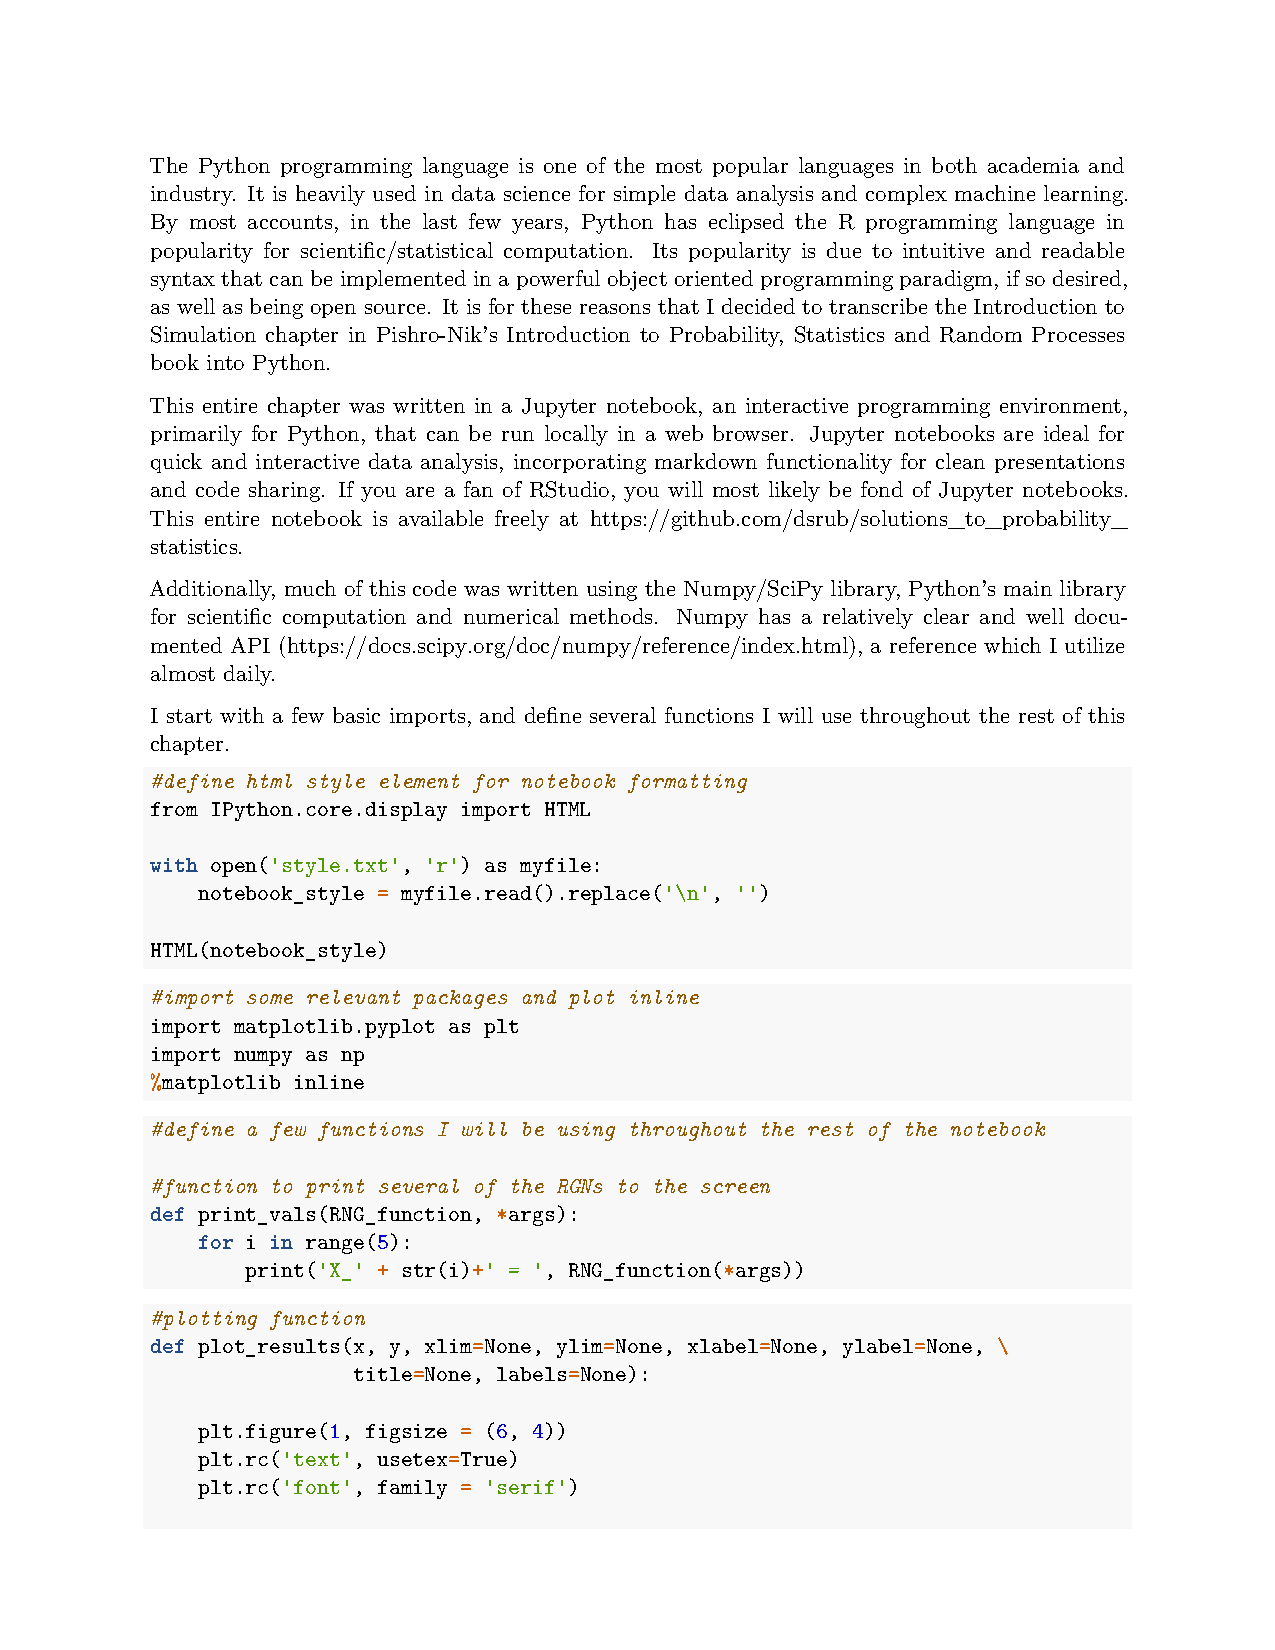
\includepdf[pages={1-}, pagecommand={}]{chpt12/chapter_12.pdf}

\chapter{Recursive Methods}
\begin{problem}{1} $ $

	\begin{enumerate}
		\item The characteristic polynomial for this recursive formula is
		
		\begin{equation*}
		x^2-2x+\frac{3}{4}=0,
		\end{equation*}
		which has roots 1/2 and 3/2, and therefore:		
		\begin{equation*}
		a_n=\alpha \left(\frac{3}{2} \right)^n+\beta \left(\frac{1}{2} \right)^n.
		\end{equation*}
		Using the initial conditions $a_0=1$ and $a_1=-1$ leads to $\alpha=-1$ and $\beta=1$.  Thus, the solution to the recurrence equation is:
		\begin{equation*}
		a_n=-\left(\frac{3}{2} \right)^n+ \left(\frac{1}{2} \right)^n.
		\end{equation*}
		
		\item  The characteristic polynomial for this recursive formula is
		
		\begin{equation*}
		x^2-4x+4=0,
		\end{equation*}
		which can be factored into $(x-2)^2=0$.  The polynomial thus has one root, $x=2$, with a multiplicity of 2, and therefore:
		\begin{equation*}
		a_n=\alpha 2^n+\beta n 2^n.
		\end{equation*}
		Using the initial conditions $a_0=2$ and $a_1=6$ leads to $\alpha=2$ and $\beta=1$.  Thus, the solution to the recurrence equation is:
		\begin{equation*}
		a_n=2n^{n+1}+n2^n.
		\end{equation*}

	\end{enumerate}

\end{problem}


\begin{problem}{2} $ $

	\begin{enumerate}
		\item Let $A_{n,k}$ be the event of observing exactly $k$ heads out of $n$ coin tosses, and let $H$ denote the event that the last coin toss is a heads.  By conditioning on the last coin toss I obtain:
		\begin{align*}
		P(A_{n, k}) &= P(A_{n, k}|H)p+P(A_{n, k}|H^c)(1-p) \\
		&= P(A_{n-1, k-1})p+P(A_{n-1, k})(1-p),
		\end{align*}
where the equality follows because if the last coin toss is heads, then we need exactly $k-1$ heads from the first $n-1$ tosses, and if the last coin toss is tails, then we need exactly $k$ heads from the first $n-1$ tosses.  Converting this to the notation used in the problem:
		\begin{equation*}
		a_{n,k}= a_{n-1, k-1}p+a_{n-1, k}(1-p)
		\end{equation*}
$\implies$
		\begin{equation*}
		a_{n+1,k+1}= a_{n, k}p+a_{n, k+1}(1-p).
		\end{equation*}

\item We recognize that this is precisely a binomial experiment, so the probability associated with exactly $k$ heads out of $n$ is given by $\binom{n}{k} p^k (1-p)^{n-k}$, and therefore, using the equation above,
		\begin{equation*}
		\binom{n+1}{k+1} p^{k+1} (1-p)^{(n+1)-(k+1)}= p\binom{n}{k} p^k (1-p)^{n-k}+(1-p)\binom{n}{k+1} p^{k+1} (1-p)^{n-(k+1)},
		\end{equation*}
which, when simplified results in:
		\begin{equation*}
		\binom{n+1}{k+1}= \binom{n}{k}+\binom{n}{k+1}.
		\end{equation*}
We need the restriction that $0 \le k <n$ to hold for this equation to be true, since the original recursion relation does not hold if $k = n$ (in that case the last flip cannot be a tails since we need all flips to be heads, so that the $P(A_{n, k}|H^c)$ term should be 0).
\end{enumerate}
\end{problem}

\begin{problem}{3} Let $A$ be the desired event and let $q=1-p$ be the probability of tails.  To solve this problem, I first condition on whether the first toss is a heads or tails:
\begin{equation*}
P(A) = P(A|H)p+P(A|T)q.
\end{equation*}
To help solve for $P(A|H)$, I now condition on the second toss:
\begin{align*}
P(A|H) &= P(A|HH)p+P(A|HT)q \\
&= 1\cdot p+P(A|T)q,
\end{align*}
where $P(A|HH) =1$ since if you flip 2 consecutive heads, the experiment is done and where $P(A|HT) = P(A|T)$, since the first heads does not matter because we are interested in 2 consecutive heads, and 1 isolated heads does not get us any closer to the event $A$.

To help solve for $P(A|T)$, I also condition on the second toss:
\begin{align*}
P(A|T) &= P(A|TH)p+P(A|TT)q \\
&= P(A|H)p +0\cdot q,
\end{align*}
where $P(A|TT) =0$ since if you flip 2 consecutive tails, the experiment is done (and the desired even did not occur) and where $P(A|TH) = P(A|H)$, for essentially the same reason that $P(A|HT) = P(A|T)$ as described above.

I now re-express these 3 equations in slightly more readable notation:
 \[
\left\{
                \begin{array}{ll}
                 a= a^H p +a^Tq\\[10pt]
                 a^H= p +a^Tq\\[10pt]
                  a^T= a^H p,
                \end{array}
              \right.
  \]
and we see that we have a system of 3 equations with 3 unknowns.  Solving for $a$ and plugging $q=1-p$ back in I find that:
\begin{equation*}
a = \frac{p^2(2-p)}{1-p(1-p)}.
\end{equation*}
As a check, we know that in the limit that $p$ goes to 1, this expression should evaluate to unity (we definitely get $HH$ before $TT$) and in the limit that $p$ goes to 0 this expression should evaluate to 0 (we definitely get $TT$ before $HH$).  Indeed it is easily to check that this expression satisfies these 2 limits.

\end{problem}


\begin{problem}{4}  Let $A_n$ be the event that the number of heads out of $n$ tosses is divisible by 3, $p$ be the probability of heads and $q=1-p$ be the probability of tails.  To solve this problem recursively, I first condition on whether the first toss is a heads or tails:
\begin{align*}
P(A_n) &= P(A_n|H)p +P(A_n|T)q\\
& = P(A_n|H)p+P(A_{n-1})q.
\end{align*}
Here, $P(A_n|T)=P(A_{n-1})$ since if the first toss is a tails, as in the sequence below, we have observed no heads,  
\begin{center}
$\underset{\scalebox{0.6}{$n$}}{\underline{T}}$ $\underset{\scalebox{0.6}{$n-1$}}{\underline{\phantom T}}$ $\underset{\scalebox{0.6}{$n-2$}}{\underline{\phantom H}}$   $\ldots$$\underset{\scalebox{0.6}{$1$}}{\underline{\phantom H}}$
\end{center}
so that the experiment just starts over at 1 less total flips ($n-1$), and is equivalent to the sequence below:
\begin{center}
$\underset{\scalebox{0.6}{$n-1$}}{\underline{\phantom T}}$ $\underset{\scalebox{0.6}{$n-2$}}{\underline{\phantom H}}$   $\ldots$$\underset{\scalebox{0.6}{$1$}}{\underline{\phantom H}}.$
\end{center}
The numbers below the sequence $n$, $n-1$, $n-2$, $\ldots$ show the number of flips remaining before you make that particular flip.  

To solve for $P(A_n|H)$, I condition on the second toss: 
\begin{align*}
P(A_n|H) &= P(A_n|HH)p+P(A_n|HT)q \\
& = P(A_n|HH)p+P(A_{n-1}|H)q.
\end{align*}
Here, $P(A_n|HT)=P(A_{n-1}|H)$ since the the probability of $A_n$ for the sequence below, 
\begin{center}
$\underset{\scalebox{0.6}{$n$}}{\underline{H}}$ $\underset{\scalebox{0.6}{$n-1$}}{\underline{T}}$ $\underset{\scalebox{0.6}{$n-2$}}{\underline{\phantom H}}$   $\ldots$$\underset{\scalebox{0.6}{$1$}}{\underline{\phantom H}}$
\end{center}
is the same as the probability of $A_n$ for a sequence that starts with 1 heads with $n-1$ flips:
\begin{center}
$\underset{\scalebox{0.6}{$n-1$}}{\underline{H}}$ $\underset{\scalebox{0.6}{$n-2$}}{\underline{\phantom T}}$ $\ldots$$\underset{\scalebox{0.6}{$1$}}{\underline{\phantom H}}.$
\end{center}

Finally, to solve for $P(A_n|HH)$, I condition on the third toss: 
\begin{align*}
P(A_n|HH) &= P(A_n|HHH)p+P(A_n|HHT)q \\
& = P(A_n-3)p+P(A_{n-1}|HH)q.
\end{align*}
Here, $P(A_n|HHT)=P(A_{n-1}|HH)$ since the the probability of $A_n$ for the sequence below, 
\begin{center}
$\underset{\scalebox{0.6}{$n$}}{\underline{H}}$ $\underset{\scalebox{0.6}{$n-1$}}{\underline{H}}$ $\underset{\scalebox{0.6}{$n-2$}}{\underline{T}}$ $\underset{\scalebox{0.6}{$n-3$}}{\underline{\phantom T}}$   $\ldots$$\underset{\scalebox{0.6}{$1$}}{\underline{\phantom H}}$
\end{center}
is the same as the probability of $A_n$ for a sequence that starts with 2 heads with $n-1$ flips:
\begin{center}
$\underset{\scalebox{0.6}{$n-1$}}{\underline{H}}$ $\underset{\scalebox{0.6}{$n-2$}}{\underline{H}}$ $\underset{\scalebox{0.6}{$n-3$}}{\underline{\phantom T}}$   $\ldots$$\underset{\scalebox{0.6}{$1$}}{\underline{\phantom H}}$.
\end{center}
Also $P(A_n|HHH) = P(A_n-3)$ since, if we have already gotten 3 heads in the first 3 flips then the probability that the number of heads flipped in the sequence is divisible by 3 is the same as if the remaining $n-3$ flips is divisible by 3. 

I summarize this set of recursive equations in somewhat more readable notation:
 \[
\left\{
                \begin{array}{ll}
                 a_n^{HH} = a_{n-3} p +a_{n-1}^{HH}q\\[10pt]
                  a_n^H = a_n^{HH} p +a_{n-1}^Hq\\[10pt]
                   a_n = a_n^H p +a_{n-1}q.
                 
                \end{array}
              \right.
  \]
We see that the equations are a coupled set of recursive equations, so must be solved simultaneously by first solving for $a_n^{HH}$, then using this to solve for $a_n^H $, then using this to solve for $a_n$, iteratively until we reach the desired value of $n$.  In order to do this, we will need several initial conditions which we can easily be compute by hand.  For a sequence with $n=1$, the number of heads is divisible by 3 if we throw one tails (probability $q$).   For a sequence with $n=2$, the number of heads is divisible by 3 if we throw two tails (probability $q^2$).  For a sequence with $n=3$, the number of heads is divisible by 3 if we throw 3 tails or 3 heads (probability $p^3+q^3$):

\begin{align*}
&a_1 = q\\
&a_2=q^2\\
&a_3=p^3+q^3.
\end{align*}
For a sequence that starts with 1 head and with $n=1$, the number of heads is never divisible by 3 (probability $0$).   For a sequence that starts with 1 head and with $n=2$, the number of heads is never divisible by 3 (probability $0$).  For a sequence that starts with 1 head and with $n=3$, the number of heads is only divisible by 3 if we throw 2 heads after the first (probability $p^2$):
\begin{align*}
&a_1^H = 0\\
&a_2^H=0\\
&a_3^H=p^2.
\end{align*}
Finally, for a sequence that starts with 2 head and with $n=1$, the number of heads is never divisible by 3 (probability $0$).   For a sequence that starts with 2 head and with $n=2$, the number of heads is never divisible by 3 (probability $0$).  For a sequence that starts with 2 head and with $n=3$, the number of heads is only divisible by 3 if we throw 1 head after the first 2 (probability $p$):
\begin{align*}
&a_1^{HH} = 0\\
&a_2^{HH}=0\\
&a_3^{HH}=p.
\end{align*}

I can check this coupled set of recursive equations by recognizing that we can compute $P(A_n)$ directly using the binomial distribution and only summing over the number of successes which are divisible by 3.  This can be written as:
\begin{equation*}
P(A_n) =\sum_{k=0}^{\floor{\frac{n}{3}} }\binom{n}{3k} p^{3k}q^{n-3k}.
\end{equation*}
I wrote a python function (below) to compute $P(A_n)$ using both methods.  I compute $P(A_n)$ for a range of $n$, for several values of $p$, and plot $P(A_n)$ calculated recursively against  $P(A_n)$ calculated with the binomial distribution as well as the 45 degree line in Fig.~\ref{fig:prob_4}.  If there is perfect agreement between the 2 methods, the points should lie along this line, and indeed this is exactly what we see.

	\begin{figure}[t]
	\centering
      		 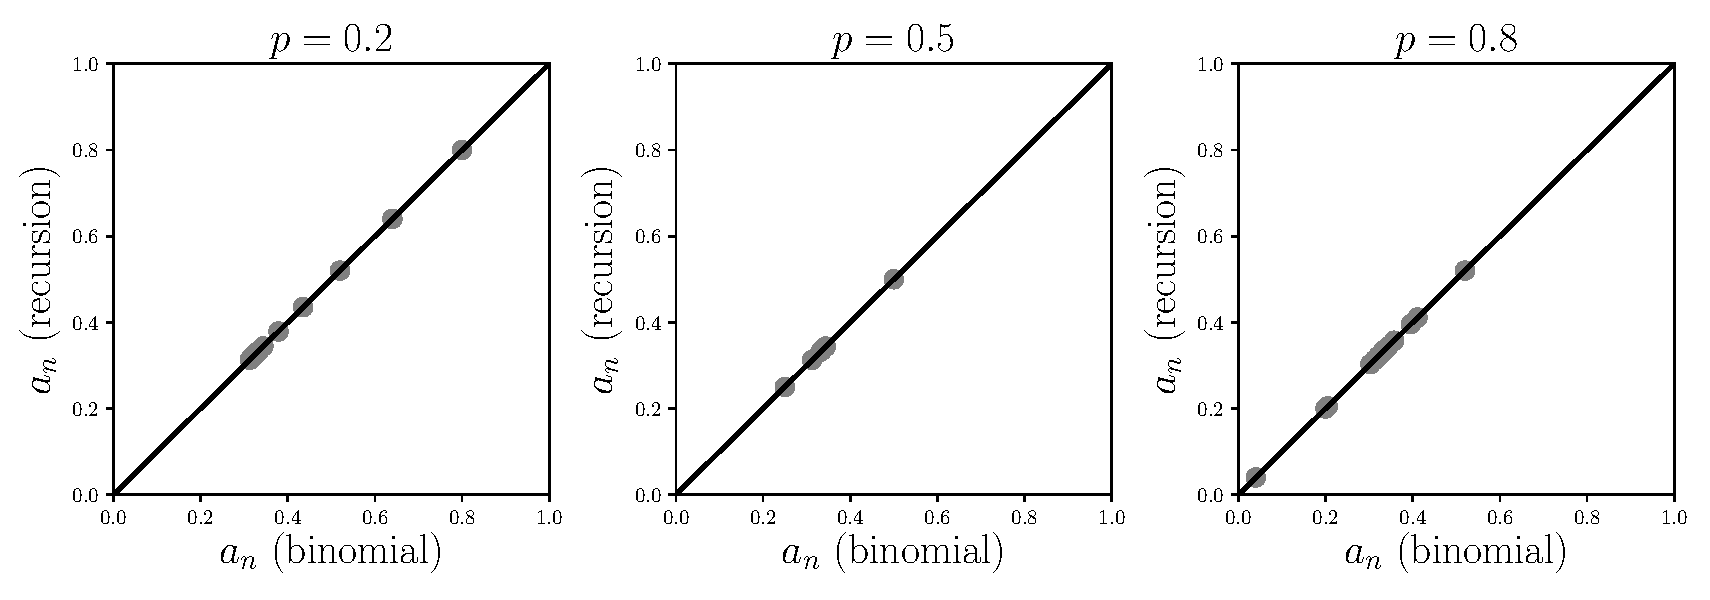
\includegraphics[totalheight=6cm]{chpt13/prob4.pdf}
  			  \caption{Comparison of $P(A_n)$ calculated recursively against $P(A_n)$ calculated with the binomial distribution (Problem 4).}
    			   \label{fig:prob_4}
	\end{figure}

\begin{lstlisting}
import numpy as np
from scipy.special import binom

def compute_binom_recur(p, N):
    """
    Compute probability that the number of heads out of N 
    coin flips (each of probability p) is divisible by 3.
    Returns the probability computed from the binomial
    distribution and the probability computed from recursion.
    """
    
    #compute the probability from the binomial
    P_arr=[]
    for n in range(1, N):
        P = np.sum(np.array([binom(n, 3*k)*p**(3*k)*(1-p)**(n-3*k)\
                             for k in range(0, int(np.floor(n/3)+1))]))
        P_arr.append(P)
     
    #compute the probability from recursion
    q = 1-p
    
    #initialize recursion
    an_HH = [0, 0, p]
    an_H = [0, 0, p**2]
    an = [q, q**2, p**3+q**3]
    
    for _ in range(N-4):
        #recursion update equations
        an_HH_new = an[-3]*p+an_HH[-1]*q
        an_H_new = an_HH_new*p+an_H[-1]*q
        an_new = an_H_new*p+an[-1]*q

        an_HH.append(an_HH_new)
        an_H.append(an_H_new)
        an.append(an_new)
        
    return (P_arr, an)
\end{lstlisting}
\end{problem}












\end{document}